\documentclass{FastFyp}
\usepackage{float}
\usepackage{longtable}
\usepackage{comment}
\usepackage{graphicx}
\begin{document}
\newcommand{\supervisor}{Usman Anwer}
\newcommand{\university}{National University of Computer and Emerging Sciences, Lahore}
\newcommand{\fyptitle}{RNA 3D Structure Prediction }
\newcommand{\degree}{BS}
\newcommand{\Studentone}{Haleema Saadia     23L-0960    BSCS} 
\newcommand{\Studenttwo}{Ansa Mubasher     23L-0580    BSCS}
\newcommand{\Studentthree}{Alizeh Adeel     23L-0674    BSCS}
\date{\today}
\renewcommand{\contentsname}{Table of Contents}
% Data dictionary tables (Section 4.9.2): header row, table row, and one captioned table per database table.
\newcommand{\hdr}{\hline \textbf{Column Name} & \textbf{Data Type} & \textbf{Column Definition} & \textbf{Nullable} & \textbf{Unique} & \textbf{Column is PK/FK} \\ \hline}
\newcommand{\rw}[6]{#1 & #2 & {\raggedright #3\par} & #4 & #5 & #6 \\ \hline}
\newcommand{\tbl}[3]{%
\par\noindent\begin{minipage}{\textwidth}% keeps each caption on the same page as its table
\begin{center}\captionof{table}[Data Dictionary: #1]{#1}\label{tab:dd-#1}\parbox{0.85\textwidth}{\centering\textit{#2}}\end{center}
\begin{center}\small\setlength{\tabcolsep}{4pt}
\begin{tabular}{|p{3.7cm}|p{2.0cm}|p{4.0cm}|c|c|p{1.5cm}|}
\hdr #3
\end{tabular}\end{center}
\end{minipage}\par\vspace{1em}}

\makeatletter
    \begin{titlepage}
        
\includegraphics[width=0.2\linewidth]{Figures/nulogo.png}\hfill
        
\includegraphics[width=0.2\linewidth]{Figures/fast.png}\\
        \begin{center} 
            {\large\bfseries \university}\\[7ex]
            
\includegraphics[width=0.4\linewidth]{Figures/fastlogo.png}\\[8ex]
            {\huge \bfseries  \fyptitle }\\[10ex] 
            {\Studentone}\\{\Studenttwo}\\{\Studentthree}\\[4ex] 
            {Supervisor: \supervisor} \\ [10ex]
            {Final Year Project}\\
            {\large \@date}
        \end{center}
    \end{titlepage}    
\makeatother
\frontmatter

\newpage \thispagestyle{empty} \mbox{} \newpage %Aatira

\pagestyle{empty}  %Aatira
\section*{\begin{center}{Anti-Plagiarism Declaration} \end{center}} %Aatira
This is to declare that the above publication was produced under the:
\begin{flushleft}
\bf Title: \fyptitle
\end{flushleft}

is the sole contribution of the author(s), and no part hereof has been reproduced as it is the basis (cut and paste) that can be considered Plagiarism. All referenced parts have been used to argue the idea and cited properly. I/We will be responsible and liable for any consequence if a violation of this declaration is determined.
\\[4ex]
Date: ..........................

\begin{flushright}
Name: Haleema Saadia
\\[3ex]
Signature: ..........................
\\[6ex]
Name: Ansa Mubasher
\\[3ex]
Signature: ..........................
\\[6ex]
Name: Alizeh Adeel
\\[3ex]
Signature: ..........................

\end{flushright}

\pagebreak

\section*{Author's Declaration}
We declare that the work presented in this report is our own, and that it has not been submitted or presented previously to any other institution or organization.
\\[4ex]
Date: ..........................

\begin{flushright}
Name: Haleema Saadia
\\[3ex]
Signature: ..........................
\\[6ex]
Name: Ansa Mubasher
\\[3ex]
Signature: ..........................
\\[6ex]
Name: Alizeh Adeel
\\[3ex]
Signature: ..........................

\end{flushright}
\pagebreak
\section*{Abstract}
Our work proposes a framework for improving template discovery in RNA 3D structure prediction. Building on RNAPro, whose accuracy depends on the quality of its input templates, we change how templates are found and chosen at inference while keeping the model fixed. We tried several template-search methods, first on their own and then together. We built two new methods from scratch, a two-tower retriever and a search over predicted structural tokens. Six other methods use existing tools: MMseqs2, Infernal with Rfam, Rfam family lookup, language-model embeddings, secondary-structure search and motif search. A learned selector trained on TM-align labels ranks all the candidates, and if none of them is useful it falls back to a zero-valued template. We compare the results with MMseqs2 alone, the first-place Kaggle search and the best-template upper bound.
\pagebreak


\section*{Executive Summary}

Predicting the 3D structure of RNA is difficult, and accuracy depends heavily on the quality of the structural templates supplied to a prediction model. Our baseline, RNAPro~\cite{leerna}, extends the Protenix AlphaFold 3 reproduction with multiple sequence alignments, an RNA language model, and 3D templates. Its authors found that templates are the model's most important input, that accuracy tracks the best available template, and that different template-search strategies succeed on different targets. Existing searches rely mainly on sequence similarity, which can miss templates whose structure is conserved where their sequence is not. This project addresses that gap: how to find and choose better templates for each RNA.

We keep RNAPro's architecture and training recipe fixed, so any improvement can be attributed to better template retrieval and choice rather than retraining. Before building any new model, a feasibility study runs the fixed model with structurally aligned oracle templates, sequence-aligned oracle templates and the existing templates, to measure how much better retrieval and alignment could help. Our contribution is a template-retrieval and selection layer applied at inference, made up of two parts. The first part is a set of template-search methods that each look for templates in a different way, and whose candidates are pooled together. Six of them use existing tools: MMseqs2 sequence search, Infernal with Rfam covariance models, Rfam family lookup, language-model embedding similarity, secondary-structure-aware search and motif search. The other two are new methods that we trained from scratch. The first new method is structural-token retrieval. A model predicts a structural token for each nucleotide, describing its local spatial-neighbour geometry, from the sequence alone. The predicted token string is searched against tokens computed from solved structures, and the token alignment gives the residue mapping onto each template. A go/no-go experiment on held-out RNA families checks that token prediction beats simple baselines before the search is built.

The second new method is two-tower retrieval with a learned aligner. A sequence encoder and a geometric structure encoder, both trained on TM-score supervision, place a sequence close to the solved structures that share its fold. A learned aligner, trained on residue correspondences from structural alignments, maps the target onto each retrieved template. We test every method on its own and as part of the pool, and keep MMseqs2 alone and the first-place Kaggle search used in the paper as baselines. The second part is a learned selector. Candidates are pooled and scored by a ranking or deep-learning model trained to predict each template's TM-align against the experimental structure, computed with US-align on the C1$'$ atom. Near-duplicates are removed, and the top five templates are passed to the trained model, which produces five predictions. If no candidate scores above a threshold tuned on validation data, a zero-valued template is used, as RNAPro does.

The last stage of the pipeline is a structure validation engine, which ranks the predicted structures because the true structure is not known at prediction time. The engine reuses gRNAde, a pretrained geometric deep learning model built for RNA inverse design, and we did not train or fine-tune it. Each candidate structure is passed through gRNAde with the true target sequence given to its decoder, and the perplexity of that sequence is used as the quality score. A structure with the right fold explains its own sequence well and gets a low perplexity, while a wrong fold gets a high one. Scores are turned into z-scores within each target, and the engine returns the top-ranked structure, a top-five shortlist and a high, medium or low confidence label. We tested it on 1,750 candidate structures submitted for 13 CASP15 RNA targets. Its top pick had a mean TM-score of 0.464, compared with 0.279 for a random pick and 0.552 for the best structure in each pool, and it beat random selection on 12 of the 13 targets (p = 0.0005).

We use PDB structures with C1$'$ coordinates, rMSA-generated MSAs, and the Eigen dataset for the second training stage. The primary benchmark uses a temporal cutoff, as in the paper. Template searches for all targets run only against structures that are legal under the split, the retrieval models are trained on data split by RNA family, and test targets are scored once. Each retrieval method is first evaluated on its own terms, through token accuracy, retrieval recall and alignment accuracy. Final performance is measured by TM-align (best of five predictions per target, averaged across targets), with a score above 0.45 indicating a correct global fold. We also report TM-score, C1$'$ RMSD, and per-target Z-scores. Results are compared against reference points from the paper, which are 0.321 for the MMseqs2-only baseline and 0.679 for the best prior PDB template (the upper bound). RNAPro's own reported mean is 0.640 in the text and 0.648 in Table 2, so we will compare against our own reproduced baseline instead. Template-poor targets are reported separately, and confidence intervals or significance tests are used where the test set size allows.

The RNAPro results are retrospective, and a prospective blind test is still needed; our evaluation inherits this limitation. Because accuracy is bounded by the best available template, the retrievers and the selector can improve results only up to that ceiling, and we will report how close they come. The retrieval models are trained from scratch on a limited number of solved RNA structures, and it is not yet established that structural tokens can be predicted from sequence alone; a method that fails its go/no-go experiment will be reported as a negative result. The paper's small test set (ten RNA-Puzzles targets) limits statistical power. Full retraining requires substantial compute (the paper used eight GB300 GPUs), so if it proves infeasible we will report the best available alternative and state this clearly. The validation engine was tested on only 13 targets, and its confidence labels were correct for 54\% of them, so more targets are needed before the labels can be relied on. Overall, this work tests whether learned template retrieval, trained from scratch to connect an RNA sequence to structurally similar solved RNAs and combined through a learned selector, improves RNA 3D structure prediction over sequence-based search, and how much of the gap to the best-template upper bound it can close.

\pagebreak


\pagestyle{fancy} %Aatira
\tableofcontents

\pagebreak
\listoffigures	% comment this if there are no figures
\addcontentsline{toc}{chapter}{List of Figures}
\pagebreak
\listoftables % comment this if there are no tables
\addcontentsline{toc}{chapter}{List of Tables}

\mainmatter


\clearpage
\chapter{Introduction}
\label{ch:intro}

RNA molecules do much more than carry genetic messages. They regulate genes, catalyze reactions and form part of the cell's machinery, and what they do depends on the shape they fold into in three dimensions. Determining an RNA structure experimentally is slow and expensive, which is why computational prediction is an active research area. Deep learning has transformed protein structure prediction, but RNA is still a harder problem. Relatively few RNA structures have been solved experimentally, and the molecules themselves are flexible and often take on more than one conformation.

One recent model for this problem is RNAPro~\cite{leerna}. It builds on Protenix, a reproduction of AlphaFold 3, and adds multiple sequence alignments, an RNA language model and 3D structural templates. Its authors found that templates are the most important of these inputs. They also found that accuracy follows the quality of the best template available, and that different template-search methods succeed on different RNAs. So no single search method works reliably for every target, and the model itself has no way of deciding which templates to trust. This project focuses on that gap. We keep RNAPro's architecture and training recipe fixed and change only how templates are found and selected at inference time. Several independent search methods propose candidates. Six of them are built on existing tools: MMseqs2 sequence search, Infernal with Rfam covariance models, Rfam family lookup, language-model embedding similarity, secondary-structure-aware search and motif search. The other two are new methods that we trained from scratch, a two-tower retriever and a search over predicted structural tokens. A learned selector ranks the pooled candidates by how accurate a structure each one is expected to give. After RNAPro has made its predictions, a structure validation engine ranks them using gRNAde, a pretrained inverse-design model that we use without any extra training, so that a good structure can be picked without knowing the true one. Since the model stays fixed, any improvement we see can be put down to better template choice and not to retraining.

\section{Purpose of this Document}
This document describes the design, methodology and planned evaluation of our Final Year Project (FYP), which aims to improve template discovery for RNA 3D structure prediction. The project is guided by the following research questions:
\begin{enumerate}
    \item Does pooling template candidates from several independent search methods, and choosing among them with a learned selector, improve prediction accuracy over a single search method?
    \item How much of the gap between the baseline and the best-template upper bound can such a selector close?
    \item Can a pretrained inverse-design model, used without any extra training, pick the best structure from a set of predicted candidates?
    \item How does performance change on template-poor RNAs, which existing benchmarks do not cover?
\end{enumerate}
The report covers the background and related work, the proposed framework, the data and splits, the evaluation protocol, and the system researchers will use to submit RNA sequences and inspect predicted structures. It also sets out the limitations of the work. The main ones are that the RNAPro results we build on are retrospective, that accuracy is capped by the best available template, and that full retraining needs substantial compute.

\section{Intended Audience}
This report is written mainly for researchers in computational biology who might use the resulting tool, and for future students or researchers who may want to extend it. We assume readers already know machine learning and software engineering. RNA structure prediction is a fairly specialized area, though, so the report explains the biological and structural concepts it relies on, and Section~\ref{sec:definitions} defines the key terms. The FYP evaluation panel is a secondary audience. Its faculty members will assess the technical soundness, novelty and completeness of the work.

\section{Definitions, Acronyms, and Abbreviations}
\label{sec:definitions}
Table~\ref{tab:defs} lists the key terms, acronyms and abbreviations used in this document.
\begin{longtable}{p{0.22\textwidth} p{0.72\textwidth}}
\caption{Definitions, acronyms, and abbreviations used in this document}\label{tab:defs}\\
\hline
\textbf{Term} & \textbf{Meaning}\\
\hline
\endfirsthead
\hline
\textbf{Term} & \textbf{Meaning}\\
\hline
\endhead
SDG & Sustainable Development Goal\\
FYP & Final Year Project\\
REST & Representational State Transfer\\
API & Application Programming Interface\\
2D & Two-dimensional\\
3D & Three-dimensional\\
3D Viewer & The in-browser tool (Mol* or NGL) used to display and interact with a predicted 3D structure.\\
Baseline Score & The score of a model before the re-ranker is applied. It is shown next to the re-ranker score so the user can see what re-ranking changed.\\
C1$'$ atom & The carbon atom of the ribose sugar used to represent each nucleotide when RNA structures are compared.\\
CASP15 & The 15th Critical Assessment of Structure Prediction, a blind community benchmark used here to test the validation engine.\\
Candidate (Top-k) & One of the k best predicted models for a sequence, as ranked by the re-ranker.\\
Confidence Indicator & A simple low, medium or high flag with a short reason, telling the user how far a predicted model can be trusted.\\
Dot-Bracket Notation & A text representation of a secondary structure in which matching brackets mark paired nucleotides and dots mark unpaired ones, e.g., ((((...)))).\\
gRNAde & A pretrained geometric deep learning model for RNA inverse design, used in this work to score predicted structures.\\
Job & A single prediction request submitted by the user. It runs in the background and produces one or more predicted models.\\
Loop & A group of unpaired nucleotides enclosed by, or connecting, stems.\\
MMseqs2 & A fast sequence search tool, used here as the baseline template search.\\
Model (3D Structure) & A predicted three-dimensional arrangement of the atoms of an RNA molecule, generated by the prediction pipeline.\\
MSA & Multiple Sequence Alignment, an alignment of related sequences that shows which positions are conserved.\\
PDB & Protein Data Bank, a standard text file format for storing 3D molecular coordinates that can be opened in external molecular tools.\\
Perplexity & A measure of how well a model predicts a sequence; a lower value means the sequence fits the structure better.\\
Pseudoknot & A structural element in which base pairs cross each other, so it cannot be drawn as a simple nested structure.\\
Re-ranker & The machine learning layer that scores candidate models and reorders them so the most likely ones appear first.\\
Researcher & The end user of the system, who submits RNA sequences and inspects the predicted structures.\\
Rfam / Infernal & A database of RNA families and the tool used to search it by sequence and secondary structure.\\
RMSD & Root Mean Square Deviation, the average distance between corresponding atoms in two structures.\\
RNA & Ribonucleic Acid\\
RNAPro & The baseline structure prediction model this work builds on.\\
RNet2 & The RNA language model used inside RNAPro.\\
Secondary Structure & The 2D pattern of base pairs formed when an RNA sequence folds, made up of stems, loops and pseudoknots.\\
Selector & The learned model that scores candidate templates and picks the most trustworthy ones for each RNA.\\
Stem & A stretch of consecutive base-paired nucleotides, shown as a double-stranded region in the 2D graph.\\
SVG & Scalable Vector Graphics, the image format used to draw the interactive 2D secondary structure graph.\\
Template & A known RNA structure used as a starting point for predicting the structure of a new sequence.\\
Template-poor target & An RNA with no close structural match in the available database.\\
Temporal split & A data split in which only structures released before a target's cutoff date can be used as templates or training data.\\
TM-align / TM-score & A measure of structural similarity between two 3D structures, ranging from 0 to 1. A score above 0.45 is treated as a correct global fold.\\
US-align & The tool used to compute TM-align for RNA structures.\\
Validation engine & The final stage of the pipeline, which ranks predicted structures with gRNAde without knowing the true structure.\\
WebGL & Web Graphics Library, the browser technology used to render 3D graphics.\\
\hline
\end{longtable}

\section{Conclusion}
In this chapter we introduced the problem. RNAPro's accuracy depends on its templates, no single search method works for every RNA, and the model cannot judge which templates to trust. Our project keeps RNAPro fixed and changes only how templates are found and chosen at inference. Eight search methods, six built on existing tools and two trained from scratch, propose candidates, and a learned selector ranks them. Since the model stays fixed, any improvement can be traced to better template choice. A validation engine based on the pretrained gRNAde model then ranks the predicted structures, so a good structure can be chosen without the true one. The work does have limits. The RNAPro results it builds on are retrospective, accuracy is closely tied to the best available template, and full retraining needs substantial compute. The rest of this report is organized as follows. Chapter~\ref{ch:vision} sets out the problem, goals, scope, constraints, business opportunity and stakeholders. Chapter~\ref{ch:litreview} reviews 15 related papers and summarizes them in a table. Chapter~\ref{ch:srs} specifies the features, requirements, assumptions, use cases, interface, database design and risks of the system. Chapter~\ref{ch:approach} describes the proposed template-selection framework, the data splits and the evaluation protocol, and Chapter~\ref{ch:design} presents the system architecture, design strategies and class diagram. Chapter~\ref{ch:impl} covers the implementation and test cases. Chapters~\ref{ch:manual} and~\ref{ch:results} will give the user manual and the experimental results, and both will be added in FYP-II. Finally, Chapter~\ref{ch:conclusions} will give the conclusions and the plan of work for FYP-II.


\clearpage

\chapter{Project Vision}
\label{ch:vision}
This chapter lays out the vision for the project. We describe the problem domain, state the problem we address and break it down into sub-problems. After that we give the goals and objectives, the scope of the work, the sustainable development goals the project supports, the constraints we work under, the business opportunity, and the stakeholders who will use or judge the system.

\section{Problem Domain Overview}
What an RNA molecule does depends on its three-dimensional structure, but working out that structure experimentally is slow and expensive. Predicting it computationally from the nucleotide sequence is therefore an important problem in computational biology. Our project focuses on one specific part of it: how to find and choose the right templates when predicting an RNA's 3D structure. A template is a previously solved structure that resembles the target RNA. Our baseline, RNAPro, predicts structures from the sequence, multiple sequence alignments, an RNA language model and templates, and its accuracy depends heavily on the quality of the templates it is given. This makes template discovery the step where prediction quality is most often won or lost. Different template-search strategies succeed on different RNAs, and the choice of templates at inference is not learned. This is the research gap we address.

We propose a framework for improving template discovery in RNA 3D structure prediction. We implement RNAPro's architecture and training recipe, and our research is about how templates are chosen at inference. Several independent search methods each propose candidate templates for the target RNA. Six of them use existing tools and cover sequence, family, embedding, secondary-structure and motif similarity, and two are new methods that we trained from scratch. The search used by the first-place Kaggle method is included as a baseline source. A selector trained on TM-align labels ranks the pooled candidates and passes the top five to the model. If none of the candidates is useful, a zero-valued template is used as a fallback. After RNAPro makes its predictions, a structure validation engine based on the pretrained gRNAde model ranks them, so a good structure can be picked without knowing the true one. For evaluation, we use temporal cutoffs, report template-poor targets separately, and compare our results against the paper's baselines and its best-template upper bound.

The framework is delivered as a web application for doctors and researchers. Users submit an RNA sequence, optionally with a dot-bracket structure, and the app validates it and runs the prediction as a background job. The result appears in an interactive 3D viewer with PDB download, alongside the top-ranked candidates with their scores next to the baseline and a low/medium/high confidence indicator. Run history, a methodology page and clear messages for failure cases such as ``no close template found'' round out the core features. Planned extras are a 2D secondary-structure viewer, a ``chat with structure'' assistant, a thermodynamic stability curve and small-molecule compatibility screening.

\section{Problem Statement}
Predicting the 3D structure of an RNA depends heavily on finding the right template, meaning a previously solved structure that resembles the target, and template discovery is still unreliable. Different search methods succeed on different RNAs, and the choice of templates at inference is not learned. So a strong model can fail on a target simply because the right template was never found, or was found but not trusted. When that happens, the user gets a poor structure with no warning. This matters because template-based modeling is becoming central to RNA 3D structure prediction, which is a core unsolved problem in biology since an RNA's structure determines what it does. Experimental determination is too slow and costly to keep up. The best strategy is a template-discovery pipeline, and ablations of the best integrated model, RNAPro, showed that templates are its most important input. The share of CASP targets with usable templates rose from 25\% in CASP15 to 56\% in CASP16, and the authors expect templates to matter even more as structural databases grow.

Our project tackles this bottleneck directly. We leave the prediction model unchanged and redesign how templates are discovered and chosen. Independent search methods based on sequence, family, embedding, secondary-structure and motif similarity pool their candidates, and a learned selector decides which ones to trust for each RNA. Since the model is held fixed, any gain can be attributed to better template choice. A validation engine then ranks the predicted structures, and we deliver the results through a web application that is honest about its confidence, so users know when a prediction can be trusted.

\section{Problem Elaboration}
This section explains the problem in more detail and then divides it into the sub-problems we work on.

\subsection{The Problem in Detail}
The problem we work on is predicting an RNA's 3D structure from its sequence, and we approach it through its main bottleneck, which is template discovery and selection. The problem has four parts. The first is that automated 3D prediction is not yet reliable. Computational methods have produced accurate predictions in blind challenges such as RNA-Puzzles and CASP, but those successes usually involved human experts guiding the modeling with literature, multiple sequence alignments, prior templates and intuition. Automated approaches, many deep learning methods included, have done worse than human experts. In the Stanford RNA 3D Folding competition, the top automated algorithms scored within statistical error of the CASP16 winners. On the ten RNA-Puzzles targets, though, they still finished just below the human expert team Vfold (0.491, 0.418 and 0.425 against 0.507 mean TM-align). Our system therefore has to take a sequence with no human in the loop and return five predicted C1$'$ structures per target that are as accurate as possible. This is the problem we are ultimately solving.

The second is that finding templates is unreliable. A prediction's accuracy follows the best template available to the model. For almost every target in the competition, a good template existed in the PDB, with 19 of 20 targets having one above a TM-align of 0.45. The hard part is finding it. The paper reports that changing the template-search strategy improved accuracy on some targets and hurt it on others. Its embedding-based search was important for an undisclosed group I intron (PZ67) but missed templates in other cases. For the RdCas12n-sgRNA-DNA complex (9J09), every approach tested did worse than a partially homologous template that was already in the PDB (TM-align 0.511, compared with 0.426 for the best model). The authors connect this to the functional relationship between target and template, which none of the Kaggle models made use of. No single search method works for all RNAs.

The third is that choosing among templates is not learned. RNAPro gets its inference templates from one fixed search procedure, the first-place Kaggle method. The only multi-model combination in the paper picked five out of fifteen predictions with a hand-built heuristic score. A heuristic like this cannot learn from data how reliable each search method is for a particular kind of RNA. Failures at this step are also silent: the model produces a confident-looking structure from a poor template, and nothing alerts the user. The fourth is that we cannot yet judge how well this works in hard cases. Almost all competition targets had templates, so the paper cautions that its conclusions in favor of template-based modeling may not hold for template-poor RNAs, which have yet to be benchmarked. Its ten RNA-Puzzles targets also limit statistical power, and its results are retrospective, so a prospective blind test is still needed. There is one more question alongside these. RNAPro returns five predicted structures for each RNA, but it gives no reliable way to tell which of them is closest to the true structure, and the true structure is not known at prediction time.

\subsection{Sub-problems}
We split the work into seven sub-problems.

\subsubsection{3D Structure Prediction}
The task here is to turn an RNA sequence into five accurate C1$'$ 3D structures without human guidance. We use RNAPro as the fixed prediction backbone. It takes the sequence, MSA, RNet2 features and templates and passes them through a 48-block Pairformer and a diffusion module to produce 3D coordinates. Its training recipe stays the same, so we reproduce the baseline and report our own number for it. At inference, each template chosen by the selector conditions one prediction. We measure the results with TM-align, TM-score, C1$'$ RMSD and per-target Z-scores. This solves the problem because the paper shows that templates are RNAPro's most important input and that accuracy tracks the best available template. This means prediction quality is limited mainly by the templates the model receives and not by its architecture. By keeping the model fixed and improving only its template input, we go straight at that limit. Any gain over our reproduced baseline can then be attributed to better templates instead of retraining, which makes the improvement both measurable and credible.

\subsubsection{Candidate Template Discovery}
No single search method finds the right template for every RNA. We run several independent search methods and pool what they find. Six of these use existing tools: MMseqs2 sequence search, Infernal with Rfam covariance models, Rfam family lookup, language-model embedding similarity, secondary-structure-aware search, and motif or local template search. The other two are new methods that we trained from scratch, two-tower retrieval with a learned aligner and structural-token retrieval. The first-place Kaggle search is added as a baseline source. For each candidate we record which method found it, along with that method's own score and rank. This solves the problem because the paper found that different search strategies work on different targets, so every method misses templates that some other method would catch. With pooling, a template only has to be found by one method to get into the candidate set, which raises the chance that the best available template is there. Function lookup and motif search also cover partial and functional homology, which is exactly the kind of case that 9J09 shows whole-sequence search can miss.

\subsubsection{Template Selection}
Pooling produces many candidates, and a hand-built rule cannot tell which ones to trust for a given RNA. We train a selector that predicts how good each candidate is, using its TM-align against the experimental structure as the label. A candidate counts as useful if its TM-align is above 0.45. The selector scores every candidate, removes near-duplicates and keeps the top matching RNAPro's five predictions per target. If no candidate clears a threshold chosen on validation data, it falls back to a zero-valued template. This solves the problem because the selector learns from training data how reliable each search method is, and for which kinds of RNA. It draws on evidence such as which method found a template, how many methods agree on it, and its sequence and secondary-structure similarity to the target. This swaps a fixed rule for a data-driven decision per RNA. The zero-valued fallback stops a poor candidate from being handed to the model as though it were trustworthy. Comparing the selector with the heuristic picker shows how much of the gain actually comes from learning.

\subsubsection{Choosing Among Predicted Structures}
RNAPro gives five predicted structures for each RNA, and the true structure is not known when one of them has to be picked. We add a structure validation engine at the end of the pipeline. It reuses gRNAde, a pretrained model built for RNA inverse design, without any extra training. For each candidate structure, gRNAde is given the target sequence, and the perplexity of that sequence is used as the score. Candidates are ranked by this score, and the engine returns the top structure, a top-five shortlist and a high, medium or low confidence label. This solves the problem because a structure with the right fold explains its own sequence well and gets a low perplexity, while a wrong fold does not. The ranking needs no reference structure, so it works on new RNAs. Since gRNAde is used exactly as it was released, the engine adds no training cost, and we can test it on a blind benchmark such as CASP15.

\subsubsection{Evaluation on Template-Poor RNAs}
Template-poor RNAs have not been benchmarked, and a temporal split by itself does not test them. This is an extension that we may add. We use two benchmarks, a temporal cutoff as in the paper and a harder structural-similarity split (planned: RNA3DB). Results on template-poor targets are reported separately. This matters because the paper cautions that its conclusions in favor of template-based modeling may not generalize to RNAs without templates. A structural-similarity split takes close structural relatives out of the template database, which gives us a test of exactly those cases. Reporting them separately means strong results on easy targets cannot hide weak results on hard ones, so we can say honestly where the framework helps and where it doesn't.

\subsubsection{Leakage-Free and Honest Evaluation}
Searching for templates over the whole PDB lets future structures leak into predictions. Every search, whether for training, validation or test targets, is restricted to structures that are legal under the split, and test targets are scored once. We report our own reproduced baseline and the distance to the upper bound, which is the best prior PDB template. Where the test set allows it, we use confidence intervals or significance tests. This is needed because if a search could see structures released after a target, the model would look accurate only because the answer was already sitting in the database. Limiting every search to legal structures means the reported accuracy reflects what the system would actually achieve on a new RNA. Comparing against our own reproduced baseline clears up the ambiguity between the paper's two figures. Measuring the distance to the upper bound shows how much of the achievable gain the selector captures, and statistical tests tell us whether differences are real given how small the test set is.

\subsubsection{Usable and Honest Delivery}
A poor prediction reaches the user without any warning. We build a web application for doctors and researchers. It validates input, runs jobs in the background, displays the 3D structure with PDB download, lists the top-k candidates with their scores next to the baseline, and shows a low/medium/high confidence indicator. Failure cases are handled explicitly, for example ``low confidence, no close template found.'' This solves the problem because the selector's scores and the template fallback give the system evidence about how far a prediction can be trusted. The confidence indicator turns that evidence into a simple signal, so a prediction built on a weak or missing template gets flagged instead of being presented as reliable. Putting the baseline score next to the re-ranked candidates lets the user see what our selector changed. Specific error messages mean failures are not silent.

Taken together, these sub-problems answer the question set out in our problem statement: whether better template discovery and selection improve RNA 3D structure prediction.

\section{Goals and Objectives}
This section gives the broad goals of the project first and then the specific objectives that follow from them.

\subsection{Goals}
Our goals for the project are listed below.
\begin{itemize}
\item Improve RNA 3D structure prediction by getting the templates right. Research has shown that templates are the most important ingredient in accurate prediction, so we aim to raise accuracy by changing how templates are found and chosen. The prediction model's architecture and training recipe stay fixed, so any gain can be attributed to better template choice.
\item Make template discovery dependable across different kinds of RNA. No single search method finds the right template for every RNA. We want a framework where several complementary methods work together, making it much more likely that the best available template is found.
\item Make template choice learned and data-driven. We aim to replace fixed or hand-built rules with a selector that learns which candidates to trust for each RNA.
\item Pick the best predicted structure without knowing the true one. We want a validation engine that ranks the predicted structures for each RNA, so users get the most reliable one first.
\item Understand what drives accuracy. We want to show which search methods help and for which kinds of RNA.
\item Evaluate honestly, including the hard cases. We aim to measure results without data leakage and report template-poor RNAs separately, so we can say clearly where our framework helps and where it does not.
\item Put it in the hands of users. We aim to build a web application where doctors and researchers can predict and examine RNA 3D structures and see how far to trust each one.
\end{itemize}

\subsection{Objectives}
\label{sec:objectives}
We turned the goals above into the following objectives, grouped by the part of the project they belong to. For prediction, we will:
\begin{itemize}
\item Train our prediction model following RNAPro's design and training recipe, and reproduce its baseline so we have a reference number of our own.
\item Produce five predicted C1$'$ structures per RNA, each guided by one of the five templates chosen by our selector.
\end{itemize}

For template discovery, we will:
\begin{itemize}
\item Build eight template-search methods: six based on existing tools (MMseqs2 sequence search, Infernal with Rfam, Rfam family lookup, language-model embedding similarity, secondary-structure-aware search, and motif or local template search) and two new methods trained from scratch (two-tower retrieval with a learned aligner, and structural-token retrieval).
\item Use the first-place Kaggle method's search as a baseline source to measure our framework against.
\item Record which method found each candidate template, with that method's score and rank.
\item Test each new method on its own to see which ones help.
\end{itemize}

For template selection, we will:
\begin{itemize}
\item Compute a TM-align label for every candidate template in the training and validation data, treating 0.45 as the threshold for a useful template.
\item Design and train a selector that predicts how good each candidate is. Its features include which method found the candidate, its score and rank, how many methods agree on it, and its sequence and secondary-structure similarity to the target.
\item Pick the top five templates per RNA after removing near-duplicates, falling back to a zero-valued template when no candidate is good enough.
\item Compare the learned selector against a simple heuristic picker to measure what learning adds.
\end{itemize}

For structure validation, we will:
\begin{itemize}
\item Build a validation engine that scores each predicted structure with the pretrained gRNAde model, without any extra training.
\item Rank the candidates for each RNA and return the top structure, a top-five shortlist and a confidence label.
\item Test the engine on a blind benchmark (CASP15) against random selection and the best structure in each pool.
\end{itemize}

For evaluation, we:
\begin{itemize}
\item Split the 1,884 RNA chains into training (1,549), validation (159) and test (176) sets. The training chains are divided into five family-held-out folds, so every selector score on a training chain comes from a model that never saw a chain of the same family (out-of-fold evaluation). The validation chains are a second check, and the test chains are held out and not used during development.
\item Report every result with and without a date filter. With the filter, a target may only use templates released before it, so no search sees a structure that was not yet available.
\item Label every query--template pair with the TM-score from US-align, normalised by the query length.
\item Measure template retrieval and selection with the mean best TM@$k$ ($k$ = 1, 5, 10), which is the TM-score of the best template among the top $k$, averaged over targets, and with hit@$k$, the share of targets with a template of TM-score 0.45 or more among the top $k$, counted over targets that have such a template at all. The pool ceiling (a perfect selector on the pooled candidates) gives the upper bound.
\item Keep a search method only if it is the sole source of a good template (TM-score 0.45 or more) for more targets than a random method that adds ten random templates per target, taking the maximum over 20 random seeds.
\item Score the predicted structures with US-align on the C1$'$ atom, with the TM-score normalised by the experimental structure. We report the TM-score of the first prediction, the best-of-5 TM-score and the share of targets whose best prediction reaches a TM-score of 0.45.
\item Compare MMseqs2 alone, the first-place Kaggle search, each of our search methods on its own, the pooled candidates with the learned selector and the pool ceiling. For structure prediction, RNAPro (released checkpoint, unchanged) is run with the first-place Kaggle templates and with the selector's templates on the same validation chains. The published RNAPro score is given for reference only, since it was measured on different targets.
\item Test every difference with a paired bootstrap over targets (2,000 resamples, 95\% confidence interval), and count the targets that are better, the same (within 0.01 TM-score) or worse.
\item Test the validation engine on 1,750 candidate structures for 13 CASP15 targets, and separately on the 6 targets with no possible overlap with gRNAde's training data. We compare it with random selection and with the best structure in each pool, using the top-1 and best-of-5 TM-score, the selection loss (best available minus top-1 TM-score), Spearman correlation within each target and over all candidates, and a Wilcoxon signed-rank test on the per-target top-1 TM-score. The confidence levels are checked with leave-one-target-out accuracy.
\end{itemize}

For the application, we will:
\begin{itemize}
\item Build a web application that accepts a sequence (pasted or uploaded, with an optional dot-bracket structure) and checks it, giving specific error messages.
\item Run submissions as background jobs with visible status and pipeline stage, and keep a run history with shareable links.
\item Show the predicted structure in an interactive 3D viewer with PDB download, and list the top-ranked candidates with their scores next to the baseline score.
\item Show a low/medium/high confidence indicator with a short reason. Edge cases such as no usable template, a failed or timed-out job, and very long sequences are handled explicitly.
\item Add a methodology page explaining how predictions are produced and where they can be weak.
\item Add secondary features: a 2D secondary-structure viewer, a ``chat with structure'' assistant, a thermodynamic stability curve, and small-molecule compatibility screening.
\end{itemize}

\section{Project Scope}
\label{sec:scope}
The scope of this project is to design and build our own system for predicting an RNA's 3D structure from its sequence, built around a new way of finding and choosing the templates that guide the prediction. Recent research showed that templates are the most important ingredient in accurate RNA structure prediction, but also that no single search method finds the right one for every RNA. Building on this, we are developing our own template-discovery framework. It searches for templates in several complementary ways, pools everything it finds, and uses a selector we design and train to decide which templates to trust for each RNA. The chosen templates then guide a structure-prediction model that we train ourselves, following the design of RNAPro \cite{leerna}. A validation engine then ranks the predicted structures, so the most reliable one can be shown first. All of this is delivered through a web application we build, where doctors and researchers can enter a sequence, see the predicted structure and see how far to trust it.

The system will allow users to:
\begin{itemize}
\item Submit an RNA sequence (pasted or uploaded), optionally with a dot-bracket secondary structure, and have it validated with specific error messages (invalid characters, length limits, mismatched structure length, unbalanced brackets)
\item Run each submission as a background job and track its status (queued, running, finished, failed) and current pipeline stage
\item Get five predicted 3D structures per sequence, guided by the templates our selector chooses
\item View the predicted structure in an interactive 3D viewer and download it as a PDB file
\item See the top-ranked candidate models with their scores next to the baseline score
\item See a low/medium/high confidence indicator with a short reason, and clear messages for edge cases such as ``low confidence, no close template found''
\item Review past jobs in a run history, reopen or re-run them, and share any run by link
\item Read a methodology page
\item View an interactive 2D secondary-structure diagram, ask questions about a predicted structure through a ``chat with structure'' assistant, see a thermodynamic stability curve across temperatures, and screen small molecules for compatibility with predicted binding pockets
\end{itemize}

On the research side, we will:
\begin{itemize}
\item Build a template-discovery framework with eight search methods: six built on existing tools (MMseqs2, Infernal with Rfam, Rfam family lookup, language-model embedding similarity, secondary-structure-aware search, and motif or local template search) and two new methods trained from scratch (two-tower retrieval and structural-token retrieval). Where good tools already exist, such as MMseqs2, Rfam and Infernal, we use them as components in our own pipeline and combine their outputs with the rest
\item Design and train a template selector that learns which templates to trust from each candidate's TM-align score, with a fallback for RNAs that have no useful template
\item Train our prediction model following RNAPro's design and training recipe, and reproduce its baseline so that every gain we report comes from our template framework
\item Build a validation engine that ranks the predicted structures with the pretrained gRNAde model, and test it on CASP15
\item Evaluate on a temporal-cutoff benchmark and a harder structural-similarity benchmark, report template-poor RNAs separately, and compare against the published baselines and the best-template upper bound
\end{itemize}

For the application, we will use Mol* for 3D display, ViennaRNA for secondary-structure and thermodynamic features, and a language model given the predicted structure's metadata for the chat assistant. The front end will be built with React and TypeScript. The back end will be a FastAPI service backed by a PostgreSQL database, and long-running predictions will go through a job queue. Section~\ref{sec:impl-web} describes this stack in detail.

By the end of the project, we will deliver the following:
\begin{itemize}
\item The template-discovery and selection framework (candidate generation, selector and fallback)
\item A trained prediction model and a reproduced baseline
\item The validation engine and the results of the evaluation, including template-poor targets
\item A working web-based application with the features listed above
\item Documentation of the methodology, design, implementation and evaluation, plus a user manual for the application
\end{itemize}

The project scope does not include:
\begin{itemize}
\item Designing a new prediction architecture. We follow RNAPro's architecture and training recipe so that gains can be attributed to our template framework
\item All-atom prediction, since the system predicts one atom (C1$'$) per nucleotide, as in the Kaggle competition \cite{leerna}
\item Large synthetic RNAs, noncanonical pairs, RNAs with multiple 3D structures, chemically modified RNAs, and nucleic-acid--protein interfaces, none of which the competition evaluated \cite{leerna}
\item Molecular dynamics simulation or any validated prediction of small-molecule binding. The drug-compatibility feature is only a lightweight scoring dashboard
\item A prospective blind test of the predictions, since our evaluation is retrospective
\item Hosting or server infrastructure beyond what development and demonstration need, and mobile applications
\end{itemize}
We will use this scope as a guide throughout the development of the project.

\section{Sustainable Development Goal (SDG)}
Our project targets SDG 3: Good Health and Well-being, and it also supports SDG 9: Industry, Innovation and Infrastructure (Figure~\ref{fig:sdg} shows the two goals this project targets). An RNA molecule's structure determines how it interacts with proteins, other nucleic acids and small molecules, so knowing that structure is useful for biological and pharmaceutical research. Determining RNA structures in the lab is slow and expensive and needs specialized expertise. That puts it out of reach for many researchers and slows down the work that leads to new treatments. Our system predicts RNA 3D structures directly from sequence and tells users how much to trust each prediction, so researchers can get an early structural picture of an RNA before committing to costly experiments. By improving how the templates behind each prediction are found and chosen, we aim to make these predictions more dependable and in this way support research toward better health outcomes (SDG 3). The project contributes to SDG 9 as well, by bringing a new approach to a hard scientific problem and offering it as an accessible web application that researchers and doctors can use without setting up their own computational infrastructure.

\begin{figure}[H]
\centering
\begin{minipage}{0.3\textwidth}
  \centering
  
\includegraphics[width=\textwidth]{Figures/E_PRINT_03.jpg}
\end{minipage}
\hspace{1cm}
\begin{minipage}{0.3\textwidth}
  \centering
  
\includegraphics[width=\textwidth]{Figures/E_PRINT_09.jpg}
\end{minipage}
\caption{SDG 3 (Good Health and Well-being) and SDG 9 (Industry, Innovation and Infrastructure)~\cite{un-sdg}}
\label{fig:sdg}
\end{figure}

\section{Constraints}
Several constraints affect what we can build and how far our claims can go.
\begin{itemize}
\item Training a structure-prediction model like this is computationally heavy. The published RNAPro recipe that we follow used eight GB300 GPUs, and we still need to confirm whether these resources will be available to us. If full retraining is not possible on our hardware, we will report the best alternative we can manage and state clearly what we used. Candidate search and selector training also have to fit within the compute we can access.
\item We have less than a year for the research, the application and the report. This limits how many search methods we can tune in depth. It also limits how many of the secondary features (2D viewer, chat assistant, stability curve, drug screening) we can build properly.
\item Our results depend on the quality of the RNA structures, MSAs and datasets we use. Every template search has to use only structures that were legally available for a given RNA, otherwise the results would look better than they really are. This restricts how we build the training, validation and test data, and the test set can only be used once.
\item Our system can be only as good as the best template that exists. If an RNA has no useful template, no selector can create one. We can improve the choice among the templates that are available, but we cannot go beyond what the database holds, so predictions for RNAs with few or no templates may be inaccurate.
\item There are only a small number of recent RNAs with known structures that we can fairly use for testing, which limits how strongly we can claim that one method beats another. Our evaluation is also retrospective, and a prospective blind test is not possible within the project.
\item The system predicts one atom (C1$'$) per nucleotide. Chemically modified RNAs, RNAs with multiple structures, large synthetic RNAs and nucleic-acid--protein interfaces are not covered.
\item Predictions can be wrong. The application has to show its uncertainty clearly, for example through the confidence indicator and the ``no close template found'' message, so users are not misled.
\end{itemize}

\section{Business Opportunity}
Knowing an RNA's 3D structure is valuable for biological and pharmaceutical research, but getting it experimentally is slow, expensive and needs specialized expertise. Many researchers and small labs simply cannot afford to determine structures for every RNA they are interested in. A tool that gives a reliable first structural picture from sequence alone, and says how far that picture can be trusted, saves time and helps researchers decide which RNAs are worth taking into the lab. This opportunity grows as experimental structure databases expand. Recent research found that templates are becoming more important to RNA structure prediction, because more solved structures mean more chances of finding a good template for a new RNA. A system that is good at finding and choosing templates is in a good position to benefit from that growth. The same ideas could also carry over to other prediction tasks that rely on finding similar known structures.

What sets our project apart is where we put the effort. We are not just building a bigger or different prediction model. We focus on the step that decides accuracy, which is finding the right templates and deciding which ones to trust. We also design the tool around honest communication, with confidence indicators and clear failure messages, so researchers and doctors know when a prediction is dependable. That is useful in a field where automated predictions have often been unreliable. This is a research-driven final year project, and we are not planning a commercial launch, so the opportunity is mostly academic and practical. The framework and web application could support research labs and pharmaceutical teams as a quick structural screening tool, and could act as a starting point for future work on RNA structure prediction.

\section{Stakeholders Description/ User Characteristics}
This section describes the people and organizations who will use the system or have an interest in the project, and what each of them needs from it.

\subsection{Stakeholders Summary}
Our main users are researchers, such as computational and molecular biologists who study RNA structure and function. They need structural models for the RNAs they work on and are comfortable with technical terms like sequences, dot-bracket notation and PDB files. They submit sequences, examine the predicted structures, compare candidate models and judge how much to trust each result. The second main group is doctors and clinical researchers who work on RNA-related questions such as therapeutic targets. They are less likely to be experts in structure prediction, so they need clear and simple explanations. They submit sequences and rely on the confidence indicator, the methodology page and the chat assistant to understand what a result means. Pharmaceutical and drug-discovery teams are secondary users. Their interest is in how small molecules might interact with an RNA structure, and they use the predicted structures and the drug-compatibility screening as an early sign of which targets deserve lab work.

Several stakeholders are involved in the project itself. Our project advisor, Mr. Usman Anwer, guides the research direction and methodology and reviews our work. The project team (Alizeh Adeel, Haleema Butt and Ansa Mubasher) designs and trains the template framework, builds the application, runs the evaluation and writes the report. FAST-NUCES, Lahore is the institution that evaluates the project as a final year project and provides academic resources for it.

\subsection{Key High-Level Goals and Problems of Stakeholders}
Researchers want an accurate 3D structure from a sequence quickly, the ability to compare several candidate structures, and a clear idea of how reliable each one is. At the moment, experimental methods are slow and costly, and automated predictions can be wrong without any warning. It is also hard for a researcher to tell whether the right template was behind a prediction. Our system deals with this by finding and choosing templates more carefully, showing the top candidates with their scores, and flagging low-confidence results. Doctors and clinical researchers want to understand an RNA's structure well enough to support their decisions, without expert knowledge of structure prediction. Raw predictions are technical and hard to interpret, it is difficult for them to tell when a result can be trusted, and they often do not have access to suitable tools. Our application helps with input validation, a plain-language methodology page, a low/medium/high confidence indicator with a short reason, and an assistant they can ask about the predicted structure.

Pharmaceutical and drug-discovery teams want an early look at an RNA's structure and possible binding pockets so they can decide which targets are worth taking to the lab. Determining structures experimentally for many candidate RNAs is too slow and expensive, and weak predictions waste effort. The predicted structure, pocket information and drug-compatibility score give them a quick first screen, and the confidence indicator warns them when a prediction should not be relied on. Our project advisor wants a well-founded research contribution backed by an honest, reproducible evaluation. The risk here is results that are overstated, leak test data or cannot be repeated. This is why we restrict every template search to structures that were legally available, score the test set only once, report template-poor RNAs separately and compare against our own reproduced baseline. As the project team, we want to finish a working framework, evaluation and application within the time and compute we have. The university expects a complete, well-documented project that meets academic standards, with a working demonstration and an evaluation that can be checked. Our documentation, user manual and results chapters are intended to meet this.

\section{Conclusion}
This chapter defined the problem our project addresses, which is finding and choosing the right templates for RNA 3D structure prediction. RNAPro's accuracy depends strongly on its templates, yet the way it chooses them is not learned. Our goals follow from this. We keep the prediction model fixed, pool several template-search methods, choose among their candidates with a learned selector, rank the final predicted structures with a validation engine, evaluate without data leakage, and provide a web application for researchers and doctors. The scope is limited to predicting one C1$'$ atom per nucleotide and leaves out chemically modified RNAs, RNAs with multiple structures, large synthetic RNAs and nucleic-acid--protein interfaces. Constraints on compute, time and data fairness, along with the ceiling set by the best available template, shape what we can claim. The project supports SDG 3 and SDG 9, and its opportunity is mostly academic and practical. The next chapter reviews the related work.

\clearpage



\chapter{Literature Review / Related Work}
\label{ch:litreview}
This chapter reviews the research our project builds on. Our work is about improving template discovery for RNA 3D structure prediction, so the review looks at two questions:
\begin{enumerate}
\item What is the best way to predict RNA 3D structure from sequence?
\item Which ways of finding and choosing templates have already been tried?
\end{enumerate}

We reviewed 15 papers in total:
\begin{itemize}
\item The Stanford RNA 3D Folding competition study, which introduced RNAPro, our baseline.
\item Models that predict RNA 3D structure directly: RhoFold+, DRfold2, epRNA, trRosettaRNA and trRosettaRNA2.
\item A structure search method: RiboSeek.
\item RNA language models and their uses: RiNALMo, BioLLMNet, and the attention study by Papazoglou et al.
\item Inverse-folding models, which work in the other direction, from structure to sequence: the model by Ding and Xiao, RiboDiffusion and gRNAde.
\item Cell2Sentence, a framework for applying language models to single-cell biology.
\item A review of machine learning for RNA structure prediction.
\end{itemize}

We start by defining the terms used in the chapter. Section~\ref{sec:detailedlit} then goes through the papers one by one, giving a summary of each, its strengths and weaknesses, and how it relates to our work. Table~\ref{tab:litsummary} summarises all 15 papers. They are listed in the same order as the bibliography, so the numbers in the table match the reference list. The chapter ends with a conclusion that brings out the gaps our approach addresses.

\section{Definitions, Acronyms, and Abbreviations}
Table~\ref{tab:litdefs} lists the extra terms used in this chapter. Terms already given in Table~\ref{tab:defs}, such as RNA, MSA, PDB, RMSD and TM-score, are not repeated here.
\begin{longtable}{p{0.22\textwidth} p{0.72\textwidth}}
\caption{Definitions, acronyms, and abbreviations used in this chapter}\label{tab:litdefs}\\
\hline
\textbf{Term} & \textbf{Meaning (as used in this chapter)}\\
\hline
\endfirsthead
\hline
\textbf{Term} & \textbf{Meaning}\\
\hline
\endhead
ncRNA / lncRNA / miRNA / mRNA & Non-coding RNA / long non-coding RNA / microRNA / messenger RNA.\\
3D structure prediction & Predicting the three-dimensional coordinates of an RNA from its sequence. In the target competition, one C1 coordinate per residue.\\
Inverse folding / inverse design & The reverse of structure prediction: designing a nucleotide sequence that folds into a given 3D backbone.\\
Template-based modelling (TBM) & Predicting a structure by retrieving experimentally solved structures that share a fold with the target and using them as templates.\\
Re-ranking layer & A learned ML component that scores and orders candidate 3D structures so the best can be selected without knowing the true structure.\\
Agentic orchestration & The component of the proposed pipeline that coordinates template finding, candidate generation, language-model features, and re-ranking.\\
Language model (LM) & A model pretrained on large sequence collections (here RNA, protein, or small-molecule data) whose embeddings serve as features.\\
Embedding & Vector representation of a sequence or residue produced by a pretrained model.\\
Frozen / fine-tuned & Pretrained weights kept fixed / further trained on a downstream task.\\
Gated fusion & Combining two embeddings with a sigmoid gate (Eq.~3.1 in BioLLMNet) instead of concatenation or averaging.\\
GDT-TS, LDDT & Further structure-accuracy measures used in the reviewed evaluation protocols.\\
pLDDT & Per-residue confidence estimate of a predicted structure, used by RhoFold+ as a confidence signal.\\
F1, MCC, AUC, MAE & F1 score, Matthews correlation coefficient, area under the ROC curve, mean absolute error.\\
INF & Interaction network fidelity, reported by DRfold2 for non-canonical base-pair modelling.\\
Top-K / best-of-five & Evaluating the best among K predicted structures; the competition scores the best of five predictions per target.\\
CD-HIT / CD-HIT-EST & Tools for removing sequence redundancy by identity threshold (e.g., 80\%).\\
BGSU & Representative RNA structure set (v3.309) used by Ding and Xiao.\\
RNAcentral, Rfam, bpRNA, RNAStralign, ArchiveII & Sequence and structure databases/benchmarks used by the reviewed papers.\\
MLP, CNN, ResNet, GNN, VAE & Multilayer perceptron, convolutional neural network, residual network, graph neural network, variational autoencoder.\\
GVP & Geometric Vector Perceptron, a geometry-aware encoder used by Ding and Xiao.\\
IPA & Invariant point attention, used in the structure modules of RhoFold+ and DRfold2.\\
RoPE, SwiGLU & Rotary position embeddings and the SwiGLU activation, used in RiNALMo.\\
RNAPro-EBA & RNAPro's embedding-based template discovery using RNet2 features.\\
Protenix & Structure-prediction backbone into which RNAPro injects language-model representations.\\
RiNALMo & 650M-parameter RNA language model (Peni\'c et al.).\\
RhoFold+, DRfold2, RCLM, CSOR & RNA 3D predictor (Shen et al.); RNA 3D predictor (Li et al.); its composite language model; its clustering/scoring/refinement post-processing.\\
RiboSeek, RS-20, RS-80 & Foldseek-style RNA structure search; its 20-state geometric alphabet and the 80-state alphabet that adds nucleotide identity.\\
RiboDiffusion, gRNAde & Inverse-folding models (diffusion-based; geometric-graph-based).\\
C2S & Cell2Sentence, a framework that converts gene-expression profiles into text for language models.\\
\hline
\end{longtable}

\section{Detailed Literature Review}\label{sec:detailedlit}
This section reviews prior work on RNA 3D structure prediction, grouped by paper. Each paper is discussed in the text, and a summary table of the papers reviewed, with their references, follows. Together they show where existing methods leave gaps that our approach addresses.

\subsection{Template-Based RNA Structure Prediction Advanced through a Blind Code Competition}
Lee, He et al.\ \cite{leerna} (a bioRxiv preprint, not peer reviewed) report the outcome of the Stanford RNA 3D Folding Kaggle code competition. More than 1700 teams submitted algorithms, which were run on hidden test structures with no humans in the loop. The competition used 43 previously unreleased structures: 23 targets in a training phase and 20 ``future'' targets in a final Private leaderboard. Each algorithm had to give five predictions per target, using one C1$'$ atom per nucleotide. Predictions were scored by TM-align and averaged across targets, and a TM-align above 0.45 corresponds to a correct global fold.

There were four baselines: AlphaFold~3 run with rMSA alignments, the human expert group Vfold, the trRosettaRNA server and a simple MMseqs2 template workflow. On all 20 final targets, the top three teams (john, odat, Eigen) scored 0.578, 0.562 and 0.543, which is significantly better than AlphaFold~3 and trRosettaRNA (p $<$ 0.05). Ten of the targets were also posed as RNA-Puzzles. On these, the three teams scored 0.491, 0.418 and 0.425 against 0.507 for Vfold, and this difference was not statistically significant. Interestingly, the top two algorithms used template-based modelling (TBM) without relying on deep learning, while other top teams retrained Protenix, an open reproduction of AlphaFold~3.

After the competition, the authors combined these ideas into a single model, RNAPro. It extends Protenix with MSAs, features from the frozen RNA language model RNet2, and 3D templates. RNet2's per-layer single and pair representations are combined by weighted averaging and injected through sigmoid gating modules. Distogram features from C1$'$ templates are added to the pair representation. In the ablation, templates turned out to be the most important input. At inference, templates found by john's method give five distinct predictions. An exploratory variant, RNAPro-EBA, finds templates through embedding-based analysis with RNet2 features instead.

RNAPro reached a mean TM-align of about 0.64 on the Private leaderboard (0.640 in the text, 0.648 in Table~2), higher than any individual Kaggle model. The authors also built a weighted agentic tree-search ensemble of Protenix, Boltz and TBM predictions, which scored about 0.63 (0.635 in the text, 0.630 in Table~2). They argue that TBM is becoming more important: 19 of the 20 final targets (95\%) had a potential template with TM-align above 0.45, compared with 3 of 12 (25\%) in CASP15 and 19 of 34 (56\%) in CASP16.

The paper's main strengths are the rigour of its evaluation and the openness of the work. Test sequences and structures stayed confidential, the final targets were released only after the training phase closed, and half of them were also run as blind RNA-Puzzles for human experts. Rankings were checked under several metrics (TM-align, TM-score, C1$'$ RMSD and their Z-scores) with significance tests. The Kaggle algorithms are open source and documented. The variety among the top solutions is also what made the post-competition synthesis possible, and the authors report ablations and per-target failure cases instead of only averages.

There are weaknesses, however:
\begin{itemize}
\item The RNAPro results are retrospective, and the authors themselves say a prospective blind evaluation is needed.
\item Since 95\% of targets had templates, the conclusions in favour of TBM may not hold for template-poor RNAs.
\item With only ten RNA-Puzzles targets, the statistical power of the comparison against Vfold is limited.
\item Results were unstable across choices. Changing the number of training steps or the template search strategy helped some targets and hurt others. RNAPro-EBA helped on the group I intron PZ67 but missed templates elsewhere.
\item For target 9J09, every method did worse than a partially homologous prior template (0.426 against 0.511).
\item The agentic ensemble relies on a hand-set weighted heuristic (Protenix 0.75, TBM 0.15, Boltz 0.10) and was guided by Private leaderboard scoring. It is therefore not a selection method that works independently of the ground truth.
\item The competition did not evaluate noncanonical pairs, confidence estimation, multiple conformations, modified RNAs, small-molecule binding or protein interfaces.
\end{itemize}

This paper is the direct basis for our work. We re-implement RNAPro and extend its template-finding component, and the gaps the paper reports line up with our proposed extensions:
\begin{itemize}
\item Templates are the most important input, yet finding them is still inconsistent. No single strategy found templates across all targets, and for 9J09 no strategy matched the best prior template. This motivates testing alternative or combined template retrieval. Examples are embedding-based retrieval with other language-model features (for example RiNALMo, as a hypothesis to test) and a second-stage re-ranker over candidate templates (RiboSeek, also a hypothesis). The authors themselves suggest that adding functional annotations and publications could improve template search, and an agentic orchestration component is a natural place to do this.
\item RNAPro produces its five predictions from the top five templates without any learned ranking, and the agentic ensemble selects by fixed weights. This is the unresolved selection problem described in Sections~\ref{sec:rhofold} and~\ref{sec:drfold2}, and it is what our learned re-ranking layer targets.
\item The competition protocol shapes our evaluation: best-of-five TM-align on hidden, post-cutoff targets, along with TM-score, RMSD and significance tests. The competition also ran offline notebooks with no internet access, so for any language model we add, we must check its runtime and whether its weights are available.
\item The authors' stated limitations, especially template-poor targets and the lack of confidence estimation, show where our extended pipeline should be tested and reported.
\end{itemize}

\subsection{RiboSeek: Spatial-Neighbour Encoding for Fast RNA 3D Structure Search}
Wang et al.~\cite{wang2026riboseek} (a bioRxiv preprint, not yet peer reviewed) propose RiboSeek, a Foldseek-style framework that turns RNA 3D structure comparison into sequence-style alignment over a discrete structural alphabet. The motivation is speed. Exhaustive pairwise alignment with US-align is too slow for searching whole databases. Earlier RNA structural alphabets (SARSA, iPARTS, R3D-BLAST, iPARTS2, R3D-BLAST2) describe each residue only through the backbone pseudo-torsions $\eta$ and $\theta$.

RiboSeek takes a different approach and represents each nucleotide with SE(3)-invariant descriptors:
\begin{itemize}
\item sequential inter-residue distances;
\item base-plane angles;
\item for each of the three nearest non-sequential C1$'$ neighbours within 12~\AA, a distance, a base-normal angle and a base-centroid direction angle;
\item a non-sequential contact count.
\end{itemize}

The production 15-dimensional vector drops $\eta$ and $\theta$. K-means with $K = 20$, fitted on a family-held-out pool of 3{,}419 chains, gives the geometric alphabet RS-20. RS-80 combines each RS-20 state with the nucleotide identity (a four-letter base channel), and its substitution matrix weights the base-match term by $\alpha = 2$. For search, a spaced-seed prefilter on RS-80 passes 500 candidate chains to C-implemented Needleman--Wunsch and Smith--Waterman alignment. The two z-score-normalised scores are then summed.

In a family-held-out ablation, the three spatial-neighbour features alone reach an AUC of 0.945, against 0.921 for all seven traditional backbone and base features. Removing $\eta$ and $\theta$ from the combined vector raises the AUC further, to 0.955. The main benchmark is an 11{,}170-pair, length-matched, hard-negative Rfam set (8{,}170 same-family positives and 3{,}000 different-family negatives). There, RS-80 reaches an AUC of 0.935 and RS-20 reaches 0.898, against 0.860 for BLAST, 0.860 for iPARTS2, 0.835 for R3D-BLAST2 and 0.873 for an RNA-adapted Foldseek control.

On 600 chain pairs, RS-20 has the highest Pearson correlation with US-align TM-score: 0.830, against 0.814 for RS-80, 0.672 for BLAST and 0.648 for iPARTS2. In retrieval (156 queries against 1{,}041 chains), RS-80 reaches a recall@1 of 0.962. One query over the 15{,}391-chain experimental database takes 204~ms, roughly 75{,}000 times faster than exhaustive US-align. The authors also fold 3{,}680 Rfam families that have no experimental structures using RhoFold+, then search them against the experimental database. This gives eight strict cross-family candidate pairs and five recurrent ``hub'' chains.

The paper has several strengths:
\begin{itemize}
\item A clear ablation showing that neighbour geometry carries more family-level signal than backbone pseudo-torsions.
\item A family-held-out protocol for fitting the codebook.
\item Length-matched negatives, which remove a simple shortcut.
\item Two alphabets for two purposes: RS-20 for geometric fidelity and RS-80 for retrieval.
\item Speed and simplicity, since it needs no learned encoder.
\end{itemize}

There are weaknesses, however. The work is a preprint, and the code is not yet public (the authors say it is available on request). Most baselines other than BLAST were re-implemented by the authors inside their own alignment framework. The Foldseek control uses an ad hoc atom and residue mapping instead of a retrained model.

The headline speed also comes at a cost. It depends on a prefilter whose own candidate recall is only 0.645 at $K = 10$, so sensitivity is traded for speed. The benchmarks measure Rfam family discrimination and agreement with TM-score, not whether the retrieved structures improve downstream 3D prediction. Performance also drops on long, multi-domain RNAs. For predicted libraries, the median TM-score of RhoFold+ single-sequence predictions against experiment is only 0.40, below the usual 0.5 same-fold threshold. The authors themselves describe the cross-family findings as candidate relationships, not established results.

RiboSeek deals with structure-to-structure search, not 3D structure prediction, so it relates only indirectly to our work. Its relevance is this: template-based modelling depends on retrieving experimental structures that share a fold with the target, and RiboSeek offers a fast, residue-level, alignment-based way to compare structures. Unlike the pooled global embedding in BioLLMNet, it keeps residue-level correspondence, which is what template discovery needs. The main obstacle is that RiboSeek needs a 3D query, while at template-finding time we only have a sequence. The query would have to be a predicted structure, and the authors show that retrieval from predicted queries against the experimental database is weaker than in the predicted-to-predicted setting. So RiboSeek is unlikely to replace sequence- or embedding-based first-stage retrieval such as RNAPro-EBA.

We could test two uses. The first is as a second-stage re-ranker over candidates that have already been retrieved. The second is as a cheap proxy for TM-score, given its correlation with US-align, for clustering or de-duplicating candidate templates. Both are our hypotheses to test, not results from the paper. RiboSeek is therefore best cited as evidence that neighbour-aware residue encoding supports fast structural retrieval. It should not be cited as a template-search method for sequence-only queries.

\subsection{Accurate RNA 3D Structure Prediction Using a Language Model-Based Deep Learning Approach}\label{sec:rhofold}
Shen et al. \cite{ref:Shen:2024} studied RNA 3D structure prediction from sequence alone. They introduced RhoFold+, a fully automated, end-to-end deep learning pipeline for single-chain RNAs. It combines RNA-FM, a 12-layer language model pretrained on about 23.7 million non-coding RNA sequences, with multiple sequence alignment features. A transformer module (Rhoformer) fuses the two, and the result is refined over ten recycling iterations. An invariant point attention structure module then predicts local frames and torsion angles to produce full-atom coordinates.

Training data was scarce, so the model was trained on 782 non-redundant sequence clusters from the PDB plus a self-distillation set of pseudo-labelled structures. On RNA-Puzzles, RhoFold+ reached a mean RMSD of 4.02~\AA{}, compared with 6.32~\AA{} for the second-best method, FARFAR2. On CASP15 natural RNA targets it outperformed other deep learning methods, including AlphaFold3, DRfold, DeepFoldRNA and trRosettaRNA. On a blind set of 76 newly released structures, it reached a mean RMSD of 7.74~\AA{}, and inference took about 0.14~s per structure, not counting the MSA search.

The study's main strengths are its automation, its speed and its thorough evaluation. The evaluation covers community benchmarks, blind testing, and cross-fold, cross-family and cross-type splits designed to check whether performance holds beyond training-set similarity. Several limitations remain, though. The method relies on MSA-derived information, so how good and how available the MSAs are matters a lot for prediction quality. The reported inference speed also leaves out the time needed for MSA searching. The CASP15 comparison involved only six natural RNA targets, which limits that part of the evaluation. The method can also struggle with structural features such as helix orientation at junctions, and with harder RNA structures, including long or pseudoknotted RNAs and complex families such as group I introns.

The most relevant limitation for us concerns candidate selection. RhoFold+ can generate multiple candidate structures by sampling different MSAs. However, the reported Top-K improvements, including gains of up to about 10~\AA{}, come from picking the best candidate using the known experimental structure. In a real prediction setting, the true structure is unknown, and the paper gives no ground-truth-independent way to choose the best candidate. Automatic candidate selection is left as an open problem.

This gap matters directly for our work. Instead of relying on a single end-to-end network, we approach RNA 3D structure prediction through a pipeline that combines template-based modelling, a learned ML re-ranking layer and language-model features, with an agentic orchestration component. The re-ranking stage targets the candidate-selection problem that Shen et al. \cite{ref:Shen:2024} leave open. Their use of pLDDT as a confidence signal and of Top-K sampling helps motivate how we design that layer. Their self-distillation strategy also suggests how pretrained RNA language-model embeddings can be used when structural data is limited.

Finally, their evaluation protocol will guide how we benchmark our pipeline, with RhoFold+ as a baseline for comparison. This protocol covers:
\begin{itemize}
\item RMSD, TM-score, GDT-TS and LDDT;
\item similarity-stratified analysis;
\item explicit reporting of failure cases.
\end{itemize}

\subsection{DRfold2 Is a Deep Learning-Based Tool That Enables Efficient and Accurate RNA Structure Prediction}\label{sec:drfold2}
Li et al. \cite{ref:Li:2026} studied RNA 3D structure prediction from a single sequence, with no MSA input, and introduced DRfold2. It pairs a newly pre-trained RNA Composite Language Model (RCLM) with a denoising structure module. RCLM is an 18-block, 47-million-parameter model trained on about 30 million RNAcentral sequences. It uses a composite-likelihood loss that models pairs of masked positions jointly, instead of assuming the masked tokens are independent. Its representations feed 16 RNATransformer Blocks and an Invariant Point Attention-based Denoising Structure Module, which is trained with perturbed initial frames. Four models, each keeping 20 checkpoints, give a pool of 80 candidate structures per sequence. A post-processing protocol (CSOR) then clusters, scores, optimizes and refines these into at most five final models.

The test set had 41 targets under 400 nucleotides, filtered to exclude training RNAs with more than 80\% sequence identity. On it, DRfold2 had a higher average TM-score than RNAComposer, trRosettaRNA, RhoFold, RoseTTAFoldNA and DeepFoldRNA at every identity cutoff tested (0.350 versus 0.292 for DeepFoldRNA at the 80\% cutoff). Its TM-score (0.350) and RMSD (14.40~\AA{}) were close to AlphaFold3's (0.347 and 16.00~\AA{}), and the authors report that the differences were not statistically significant. On 25 novel-fold targets it scored 0.309 against 0.281 for AlphaFold3. A hybrid that adds AlphaFold3 conformations as an extra scoring potential reached a TM-score of 0.368 and an RMSD of 14.02~\AA{}. RCLM on its own reached 49.0\% top-L contact precision at 12~\AA{}, against 23.6\% for RNA-FM.

The study's strengths include its single-sequence input and the small size of RCLM compared with RiNALMo (650M parameters) and RNA-FM (100M). Its final models are also physically clean after refinement, and it is evaluated across identity-stratified, novel-fold and MSA-depth subsets. The authors acknowledge several limitations, though. Absolute accuracy is modest: the best TM-score is 0.368, and it falls on novel folds (0.309 against 0.350 overall). Pseudoknot recovery (56.3\%) and non-canonical base-pair modelling (INF of 0.184) are still weak, and an earlier version of the model did worse on CASP16 targets longer than 200 nucleotides. The test set is small (41 targets, with subsets of 9, 21 and 37), so the statistical comparisons rest on few samples. The most telling case is the 8DP3 cloverleaf RNA, where the correct junction direction appeared in the fifth-ranked model (RMSD 6.54~\AA{}) but not in the first-ranked one (22.05~\AA{}). The authors state that the CSOR selection step needs improvement, for example by combining it with third-party algorithms. What remains open is reliable selection among candidate structures when the correct one is already in the pool.

This is the same selection problem our learned re-ranking layer targets. Li et al. \cite{ref:Li:2026} identify it but only address it with a hand-built, energy-based scoring protocol. Their 8DP3 example gives us a concrete failure case to test a re-ranker against. Their hybrid result, where external AlphaFold3 conformations are added as an extra scoring potential without joint training, suggests that outside predictions can be brought in at the selection stage. Their comparison of RCLM with RNA-FM, RiNALMo and RNAErnie also informs our choice of language-model features. Their evaluation protocol, which uses TM-score and RMSD on identity-filtered subsets, a novel-fold subset and MSA-depth groups, gives us a template for benchmarking our pipeline, with DRfold2 as a baseline for comparison.

\subsection{BioLLMNet: A Unified Language-Model Framework for RNA-Interaction Prediction}
Abir et al.~\cite{abir2025biollmnet} propose BioLLMNet, a sequence-only deep learning framework that predicts RNA interactions with proteins, small molecules and other RNAs within one architecture. Existing methods usually rely on hand-crafted features, structural or physicochemical data, and designs built for one modality. BioLLMNet instead encodes each molecule with a pretrained language model: RiNALMo for RNA (1280-dimensional global embedding), ESM-2 for proteins (1024 dimensions, using the \texttt{[CLS]} representation) and MoleBERT for small molecules (768 dimensions). Since these embeddings differ in size, a single-layer MLP with ReLU projects the RNA embedding into the partner's dimension. RNA--RNA pairs need no projection, because both embeddings are already 1280-dimensional. The two aligned embeddings are then fused through a learnable gate,
\begin{equation}
  \mathbf{f}_{\text{combined}} = \sigma(\mathbf{g}) \odot \mathbf{f}'_1 + \bigl(1 - \sigma(\mathbf{g})\bigr) \odot \mathbf{f}'_2,
  \label{eq:biollmnet-gate}
\end{equation}
where $\mathbf{g}$ is a gate vector with the same dimension as the embeddings. The fused vector goes into a three-layer MLP prediction head. The projection, gate and head are trained jointly by backpropagation, with binary cross-entropy for classification.

The authors evaluate on three tasks. On RPI1460 (lncRNA--protein, 2,920 balanced samples, five-fold cross-validation), BioLLMNet reaches an MCC of 0.848, against 0.760 for the best baseline, RNAincoder. On RNA--small molecule binding affinity (ROBIN data, 10-fold cross-validation), it improves Pearson correlation in five of six RNA subtypes and MAE in all six. On miRNA--lncRNA interaction across three plant species, it leads in four of six train--test settings. An ablation shows that gated fusion beats concatenation and element-wise averaging, and the authors also present a case study on the RNA 2QEX-0.

The main strength is the unified, sequence-only design, which avoids structural data that is hard to get and gives consistent gains over published baselines on the RNA--protein and RNA--small molecule tasks. The ablation is clean (mean $\pm$ SD over five runs), significance tests are reported (all p $<$ .01), and the code and data are public. The architecture is also lightweight, since only small MLP parts are trained on top of the pretrained embeddings. There are weaknesses, however. Each molecule is reduced to one global vector, so residue-level information is lost, and the authors admit that cross-modal attention and joint pretraining are not used. Results on RNA--RNA are mixed: BioLLMNet falls below CORAIN on ATH-MTR (72 vs.\ 74) and GMA-MTR (84 vs.\ 93), and its best accuracy on MTR-ATH is only 68\%. The case study covers a single RNA (2QEX-0) with a very small set of non-interacting partners. The paper also claims the gate adapts ``based on input context'', but Equation~\ref{eq:biollmnet-gate} defines $\mathbf{g}$ as a learnable parameter vector, not a function of the input, so the gating appears to be fixed after training. This is our own reading of the formulation, not a point the authors make. Finally, the authors note that comparison with domain-specific tools has not been tested.

BioLLMNet is about RNA interaction prediction, not 3D structure prediction, so it relates only indirectly to our work, which re-implements RNAPro and extends its template-finding component. The most relevant overlap is the use of frozen pretrained RNA language-model embeddings with small learnable fusion modules on top. RNAPro follows a similar pattern. It keeps RNet2 frozen, combines its per-layer single and pair representations by weighted averaging, and injects them into the Protenix representations through sigmoid gating modules. BioLLMNet gives independent support for this design choice, since in its ablation a learned sigmoid gate over embeddings beat concatenation and element-wise averaging. It also shows that RiNALMo embeddings are a usable feature source for downstream RNA tasks. This makes RiNALMo a candidate alternative or complement to RNet2 in our extension, though that is a hypothesis for us to test, not a result from either paper.

For template finding specifically, RNAPro-EBA discovers templates through embedding-based analysis with RNet2 features, and it helped on some targets while missing templates on others. We could test whether RiNALMo embeddings, or a learned combination of RiNALMo and RNet2 embeddings, improve template retrieval. BioLLMNet does not address this directly. It uses one pooled global vector per molecule for pair classification, whereas template discovery depends on residue-level correspondence and structural similarity, so its pooled-embedding approach would not transfer without changes. BioLLMNet is therefore best cited as supporting evidence for using frozen language-model features with lightweight gated fusion, and not as a template-search method.

\subsection{Predicting RNA Structure Utilizing Attention from Pretrained Language Models}
Papazoglou et al.\ \cite{ref:Papazoglou:2025} asked whether the self-attention maps of pretrained nucleic acid language models can directly reveal RNA secondary and tertiary contacts, as has been shown for protein language models. They first checked the approach on proteins, using attention features from ESM2-3B and two ProtT5 models with a logistic regression classifier trained on only 20 proteins and tested on 14,988. This gave average F1 scores of 0.76--0.81. They then applied the same method to RNABERT, ERNIE-RNA, RNA-FM and RiNALMo, with DNABERT as an extra test. For tertiary structure they used 425 RNA structures filtered with CD-HIT-EST at 0.8 identity (362 for training and 63 for testing), turned into contact maps with a 9.5~\AA{} cutoff. For secondary structure they used about 30,000 structures from bpRNA, RNAStralign and ArchiveII. Attention maps were symmetrized and corrected with Average Product Correction. Each token pair was then classified as contact or non-contact using logistic regression, decision tree, random forest, multilayer perceptron and XGBoost, plus a CNN for secondary structure.

The top attention heads of RNA-FM and RiNALMo aligned with up to 55\% and 69.1\% of structural pairs, against 13.8\% for RNABERT and 10.7\% for ERNIE-RNA. Tertiary structure was a different story. Visual inspection of RNA-FM and RiNALMo attention showed no alignment with the tertiary contact map of the example molecule, and the tertiary classifiers reached at best an F1 of 0.56 and an MCC of 0.17, which the authors describe as close to random. For secondary structure, random forest classifiers trained on the full dataset with ERNIE-RNA, RNA-FM and RiNALMo attention reached F1 scores of 0.60, 0.59 and 0.62 (MCC 0.32, 0.29 and 0.35). This compares with 0.90 for SPOT-RNA, 0.87 for RNAfold and mxFold2, and 0.71 for RNA-MSM. On 33 RNA structures released from June 2022 onwards and shorter than 100 nucleotides, trRosettaRNA (average RMSD 5.0~\AA{}, TM-score 0.40) and AlphaFold3 (6.6~\AA{}, 0.34) outperformed RhoFold+ (7.1~\AA{}, 0.27), DeepFoldRNA and FarFar2/ARES. The attention-based tertiary classifiers (F1 0.58--0.59) were well below all of them (F1 0.76--0.85). The authors conclude that current nucleic acid language models do not capture structural information well in their attention, mainly because of architectural constraints.

The study's strengths include validating the method on proteins before applying it to RNA, and comparing four RNA language models and one DNA model under a single protocol with several classifiers. Its benchmark was also restricted to post-June-2022 structures and filtered for similarity to the classifier training data, and the code and datasets are public. The work has limitations, though. The tertiary dataset is small (425 structures, 63 for testing), and the state-of-the-art comparison covers only 33 structures shorter than 100 nucleotides. The secondary structure data comes from computationally derived annotations, which the authors acknowledge, and because of resource limits the protein validation used the second-largest version of each protein language model. RNA-MSM was evaluated only as a benchmark tool, not as a source of attention features, and UNI-RNA was left out because its code and weights were unavailable. Only attention weights were examined, and the authors themselves note that output embeddings may summarise sequence interactions more fully. They suggest that the gap comes from RNAcentral being about seven-fold smaller than UniProt, RNA language models being about four-fold smaller than protein language models, the four-letter RNA vocabulary, and quaternary interactions that sequence alone cannot reflect. What remains open is a language model whose attention, or whose embeddings, can support accurate RNA tertiary structure prediction.

This finding matters for our pipeline. Papazoglou et al.\ \cite{ref:Papazoglou:2025} show that attention maps from RNA language models such as RNA-FM and RiNALMo are not a reliable source of tertiary contact information. Our pipeline therefore does not depend on extracting attention. Instead, it uses language-model features as inputs to downstream learned components, a use the authors identify as unexplored for structure prediction. Their results also support keeping template-based and structure-aware components in the pipeline rather than relying on language-model representations alone. Their evaluation protocol will inform how we benchmark the pipeline, in particular the use of structures released after the training cutoff of competing methods, similarity filtering with CD-HIT-EST, and the combination of contact-based metrics (F1 and MCC) with RMSD and TM-score, with trRosettaRNA, AlphaFold3 and RhoFold+ as reference methods.

\subsection{RiNALMo: General-Purpose RNA Language Models Can Generalize Well on Structure Prediction Tasks}
Peni\'c et al.~\cite{ref:Penic:2024} introduce RiNALMo, which the authors describe as the largest RNA language model to date. It is an encoder-only Transformer with 650M parameters, 33 blocks and 1280-dimensional embeddings. It uses rotary position embeddings, the SwiGLU activation and FlashAttention-2, and each nucleotide is one token. The model was pre-trained by masking 15\% of the nucleotides and asking it to predict them. The training data was about 36M non-coding RNA sequences from RNAcentral, Rfam, nt and Ensembl. The authors removed duplicates and grouped the sequences into 17M clusters, and in each epoch every sequence came from a different cluster, which keeps each batch diverse. Training inputs were capped at 1024 tokens, with longer sequences randomly cropped. After pre-training, they attached small prediction heads and fine-tuned the model for several tasks: secondary structure, splice sites, ncRNA family classification and three mRNA translation tasks. For secondary structure, the nucleotide embeddings are paired up and passed to a small ResNet that outputs pairing probabilities. RiNALMo beat the other tools it was compared with on the in-family test and on the structurally dissimilar TestSetB. The key test was ArchiveII, where each of nine RNA families was held out once. Here RiNALMo beat RNAstructure and CONTRAfold in eight of the nine families, while the other deep learning models did not generalise. The authors say this is the first evidence that language models can generalise across families on this task. RiNALMo also beat models built for specific RNA types, such as SpliceBERT and UTR-LM.

The main strengths are the scale and careful curation of the pre-training data, and ablations showing that RoPE, SwiGLU and a larger model each improve results. The evaluation is also built around generalisation rather than only in-distribution accuracy, with family-held-out splits, comparisons against homology-based tools and a t-SNE analysis showing that embeddings cluster by RNA family. The weights and fine-tuning scripts are released. The paper has several limitations, though. It does not evaluate 3D structure prediction at all. The authors believe the embeddings could replace MSAs, by analogy with ESMFold and OmegaFold for proteins, but they present this as a future direction, not a result. Performance on telomerase RNAs was poor and unexplained, and this was the family where UFold did best. Pre-training used only non-coding RNAs, and input length was capped at 1024 tokens during training. Every downstream task also needs its own fine-tuning and prediction head, and the secondary structure metric counts pairs shifted by one position as correct. Finally, some comparisons rely on competing models that the authors fine-tuned themselves with a matching head, and Uni-RNA was not evaluated on every task.

RiNALMo is relevant to us because it concerns the language-model component of our pipeline. RhoFold+ used RNA-FM as its language model, and RiNALMo is a larger successor that reports better embeddings on structure-related tasks and is publicly released. Its embeddings could serve as sequence-level features for the re-ranking layer. Its secondary structure head could also give a predicted base-pairing pattern to check candidate 3D structures against. Unlike RiNALMo, our work targets 3D structure, and it uses the language model only as one feature source inside a candidate-generation and re-ranking pipeline, not as a standalone predictor. RiNALMo also shapes our methodology and evaluation. Its finding that deep learning models often fail on unseen RNA families supports validating the re-ranker with family-held-out or similarity-stratified splits, so that homologous train and test sequences don't make our gains look larger than they are. Its ablations on model size and positional encoding suggest testing more than one language-model backbone and comparing RiNALMo features with RNA-FM features. Some practical constraints need checking before we adopt it. The competition is a code competition, so we must confirm a 650M-parameter model's runtime and offline weight availability against the current rules. The paper also reports smaller 150M and 33M variants, and we still have to confirm which of their weights are publicly released.

\subsection{From 3D Structure to Sequence: Geometric-Graph Perceptron and Transformer Networks for RNA Inverse Folding}
Ding and Xiao~\cite{ding2025inverse} address RNA inverse folding, the task of predicting a nucleotide sequence from a given 3D backbone. Their pipeline encodes the structure with a Geometric Vector Perceptron (GVP) encoder and passes the residue embeddings through a Transformer to capture long-range dependencies. An MLP with a softmax then predicts the nucleotide at each position. The training set was built from the BGSU representative RNA set (v3.309) and PDB structures, about 6,300 structures in total. They kept single chains of 20--512 nt and removed redundancy with CD-HIT at 80 percent sequence similarity, which left about 2,500 chains. Each nucleotide is represented by the coordinates of three key atoms (C1$'$, O and N). Training uses a composite loss that weights sequence recovery at 0.8 and a structural term at 0.2. The authors also describe a variational autoencoder (VAE) that takes Gaussian inputs to generate diverse designs. To evaluate, they refold the designed sequences with DeepFoldRNA and compare the predicted and target structures using TM-score. Under 10-fold cross-validation, the model reached a recovery rate of 0.413 and a TM-score of 0.481, compared with 0.142 and 0.390 for RiboLogic and 0.213 and 0.324 for LEARNA. On selected Rfam families and six RNA-Puzzles targets, recovery ranged from about 0.32 to 0.61.

The work has three strengths. It conditions on 3D geometry rather than secondary structure alone. It curates its data with a representative set, a length filter and redundancy removal. It also closes the loop by refolding its designs, so it measures both sequence recovery and structural fidelity. Its main limitations are that the baselines are 2D-based tools applied to structures converted to 2D, and that the VAE and the structural loss term are not described clearly enough to reproduce. The evaluation also reports no variance and does not use structurally dissimilar, family-held-out splits. What remains open is the other direction. The work goes from structure to sequence, while the harder and less-solved problem is predicting 3D coordinates from sequence with stronger sequence-based models, evaluated under leakage-free conditions.

This gap is where our project sits. We address the forward problem of RNA 3D structure prediction with large language models for the Stanford RNA 3D Folding Kaggle competition. The input is a sequence, and the output is C1$'$ coordinates for each residue, scored by TM-score. Ding and Xiao's model maps structure to sequence, and ours maps sequence to structure, so the two tasks are inverses of each other. The contrast is useful. Their architecture is a geometry-aware encoder with a per-residue classification head. Our approach instead uses a sequence-based language model, optionally combined with template or retrieval information, to produce several candidate 3D structures for each target. The competition also differs from their setting because it scores the best of several predicted structures, so ranking candidates matters as much as generating them.

The paper informs our methodology, design and evaluation in three specific ways. First, its data pipeline (BGSU representative set, length filtering and CD-HIT at 80 percent) is similar to the curation used in RhoFold+~\cite{ref:Shen:2024}. We will make comparable choices when building training and validation data for the re-ranking stage, and add temporal or structure-based splits to close the leakage that their leave-one-out protocol leaves open. Second, their design--refold--compare loop supports adding a round-trip consistency feature to our re-ranker. A structure-conditioned inverse-folding model could score how well a candidate 3D structure is explained by the input sequence, in the same way RiboDiffusion~\cite{huang2024ribodiffusion} uses folding-based validation. Their C1$'$, O and N inputs would need backbone reconstruction from our single-C1$'$ output, so for this check we would use a model that accepts C1$'$-only input. Third, their evaluation gaps shape our plan. We will compare against the strongest available baselines, use family-held-out and structure-dissimilar splits, and report TM-score variance across folds. Overall, the paper serves as supporting related work and a source of design ideas for candidate verification, not as a core baseline.

\subsection{RiboDiffusion: Tertiary Structure-Based RNA Inverse Folding with Generative Diffusion Models}
Huang et al.~\cite{huang2024ribodiffusion} study RNA inverse folding, which means designing an RNA sequence that will fold into a given 3D backbone. Their model, RiboDiffusion, learns which sequences fit a fixed backbone. It starts from a random sequence and cleans it up step by step until it becomes a good candidate. Each nucleotide is described by three atoms: C4$'$, C1$'$, and N1 or N9. A graph neural network reads the 3D geometry, and a Transformer-style module handles the sequence. During training, the structure information is sometimes hidden, so the model learns to work both with and without it. At sampling time, a single weight trades accuracy against variety in the designed sequences. The authors trained on 7,322 PDB structures (20--280 nt) and added about 17,000 structures predicted by RhoFold, keeping only the high-confidence ones. They tested on groups split by sequence similarity and by structure similarity, so the test RNAs differ from the training RNAs. RiboDiffusion beat four 3D baselines (gRNAde, PiFold, StructGNN, GVP-GNN) with an average relative gain of 11 percent on the sequence splits and 16 percent on the structure splits. For example, recovery was 57.3 percent against 51.7 percent on the 0.8 sequence split. The authors also refolded the designed sequences with RhoFold and DRfold and measured C1$'$ TM-score against the original backbone.

The paper's main strengths are its global iterative generation, which refines all positions together instead of one nucleotide at a time as autoregressive models do, its principled handling of the one-to-many mapping between structure and sequence, and its explicit control over diversity. The evaluation is also careful about generalisation. It uses similarity-based splits and repeated runs, and its refolding check compares against refolds of the native sequence rather than relying on recovery alone. There are limitations, though. Native sequence recovery undervalues valid alternative sequences, and the folding validation depends on the accuracy of the folding tool, which makes its own errors. Augmenting with predicted structures may pass that tool's errors into training, and the authors found this augmentation noisy and only slightly helpful. The model conditions on a single fixed backbone, so it cannot represent conformational flexibility. Short RNAs (about 50 nt or less) are also harder to recover. Most importantly, RiboDiffusion solves the reverse of the competition task. It only tests real backbones, never checks whether it can tell a good predicted structure from a bad one, and does not predict structure from sequence.

This reversal is actually what makes it useful to us, because it allows a ground-truth-independent check on candidate structures. Our pipeline generates candidates through template-based modelling and has to choose among them without knowing the true structure, which is the selection problem left open by Shen et al.~\cite{ref:Shen:2024}. An inverse folding model can score how compatible a candidate backbone is with the query sequence, for example through how well the query sequence is recovered, or how likely it is under the model given that backbone. That compatibility signal could be an extra feature for the learned re-ranking layer, alongside language-model features and confidence estimates such as pLDDT. Unlike RiboDiffusion, our work does not design sequences, and uses inverse folding only as a scoring component inside a prediction pipeline. RiboDiffusion informs our methodology in two further ways. First, its use of predicted structures to add to scarce experimental data supports similar augmentation for training the re-ranker. Second, its in-silico folding validation, together with its diversity control, which mirrors the competition's best-of-five scoring, suggests a self-consistency check and makes a case for diverse candidate sets. Its limitations shape the design too. Its weaker performance on short RNAs suggests the re-ranking signal will be less reliable for short targets, and the fixed-backbone limitation supports keeping several candidate conformations instead of committing to one. Integration also needs care. The competition asks for one C1$'$ coordinate per nucleotide, while structure-conditioned models like RiboDiffusion usually need a richer backbone representation, so candidates would first have to be reconstructed. We still have to confirm which atoms RiboDiffusion's code expects before adopting this design.

\subsection{gRNAde: Geometric Deep Learning for 3D RNA Inverse Design}
Joshi et al.~\cite{joshi2025grnade} studied RNA 3D inverse design, the reverse of structure prediction: given a target three-dimensional backbone, the task is to generate nucleotide sequences that fold into it. They introduced gRNAde, a geometric deep learning pipeline built on the idea that a model must first understand an RNA's 3D geometry before deciding which nucleotide belongs at each position. The target structure is represented as a geometric graph, with nucleotides as nodes and their spatial relationships as edges. A geometric neural network learns a representation of this graph that captures how the nucleotides are arranged in 3D. A decoder then uses that representation to predict which nucleotide (A, C, G or U) should go at each position, producing a designed sequence. Because the model works directly on spatial relationships rather than on a flattened sequence or a 2D contact map, it can represent the geometry that decides which bases pair, stack and interact. The study's main strengths are this geometry-aware formulation and its use of a learned model in place of slow, search-based physics design. Representing RNA as a geometric graph lets the model use 3D information that sequence-only or 2D-only methods throw away. Several limitations remain, however. The method needs an accurate 3D backbone as input, so on its own it cannot predict structure from sequence. Its learning is limited by how few experimentally determined RNA structures are available for training. Recovering the native sequence is also only a proxy for success, since a designed sequence is not guaranteed to fold into the target without independent validation.

These limitations are why gRNAde is not a competing predictor for us. It works in the opposite direction, from structure to sequence. Instead, its geometric-graph representation informs how we can encode candidate 3D structures as features for the re-ranking stage. It also suggests a consistency check: a candidate structure can be scored by how well an inverse-design model recovers the input sequence from it, which gives a ground-truth-independent signal for candidate selection. Finally, its explicit treatment of 3D spatial relationships supports our emphasis on structure-aware evaluation. We use gRNAde as a reference for geometric representation, not as a baseline for comparison.

\subsection{Cell2Sentence: Teaching Large Language Models the Language of Biology}
Levine et al.~\cite{levine2024cell2sentence} studied how to apply large language models to single-cell biology. They introduced Cell2Sentence (C2S), a framework that converts gene expression data into plain text so that standard language models can be used without a custom architecture. It takes a single-cell RNA sequencing profile and ranks the genes in each cell by expression level. The ordered list of gene names forms a ``cell sentence'', which can be turned back into approximate expression values through a rank-to-expression relationship learned from the data. Pretrained GPT-2 models are then fine-tuned on these cell sentences together with natural-language text such as cell type and tissue labels, so one model can handle several tasks. These include generating cells conditioned on a cell type, predicting the cell type from a cell sentence, and generating text such as summaries from cell data. The authors argue that pretrained language models carry useful prior knowledge into biology, and that this transfer is why they do better than the same models trained from scratch.

The study's main strengths are its simplicity and flexibility. Since it reuses off-the-shelf language models and needs no specialised tokenizer, any LLM can use the biological data, and data and natural language can be combined in one model. Showing that pretrained weights help, rather than only training from scratch, is also a useful finding. Several limitations remain, however. Rank-based encoding is lossy: it discards absolute expression levels, and the finite context window forces each cell to be cut down to its top-ranked genes. The method is also designed for single-cell transcriptomics, not RNA structure, so it does not deal with spatial or structural data at all. Finally, the models are fairly small and the evaluation covers a limited set of datasets and tasks, so it is unclear how well the approach scales or generalises.

Cell2Sentence does not predict structure, so it is not a baseline for us, but both its strengths and its limitations bear on our design decisions. Its core idea, turning non-text biological data into a sequence a language model can process, informs how RNA sequences and predicted structural features can be represented for our language-model component. Its lossy-encoding and truncation problems also warn us that long RNA sequences may need careful handling. Its combination of biological data with natural-language text motivates our planned LLM assistant, which explains predicted structures from sequence-derived metadata. Finally, its finding that pretrained language knowledge improves performance when data is limited supports using pretrained RNA language-model embeddings, given how few experimental structures exist.

\subsection{Machine Learning and Language Models for RNA Structure Prediction: Progress and Perspectives}
Moyon and Marsico~\cite{moyon2026ml} review the state of the art in RNA structure prediction. They trace the field from thermodynamic free-energy minimisation, through supervised deep learning, to self-supervised RNA language models trained on millions of sequences. The review is motivated by the gap between known sequences and solved structures. RNAcentral holds tens of millions of RNA sequences, while the PDB holds only about 10,000 to 15,000 RNA-containing structures. Most of these are fragments, protein-bound RNAs or redundant entries, and fewer than about 1,000 distinct folds remain after filtering. The authors first summarise the main training and benchmarking datasets, including ArchiveII, bpRNA-1m, RNAsolo and RNA3DB, and the community benchmarks CASP15, CASP16 and the Kaggle Ribonanza challenge. They then describe the main model families: RNA-FM, a 12-layer transformer pretrained on 23.7 million non-coding RNAs, followed by RNA-MSM, RhoFold+, StructRFM and RiNALMo, as well as RibonanzaNet and its dual-tower design. Across recent benchmarks, RNA language models are competitive, with RNA-FM and RiNALMo leading on non-coding RNA classification and secondary structure prediction. Performance still drops on RNA families not seen in training. The CASP16 results show that machine learning methods struggle with noncanonical interactions, pseudoknots and long-range dependencies, and the best teams used thermodynamically informed predictions to bridge 2D scaffolds and 3D architectures. In their perspectives section, the authors argue for bringing in chemical probing signals, RNA modifications and interactions with other molecules. They also argue for generative models, such as diffusion models, that can capture the ensemble of conformations an RNA adopts.

The review's main strength is that it brings datasets, models and benchmarks together in one place. It also stresses how data leakage inflates generalisation estimates, which motivates similarity-reduced datasets such as RNA3DB. Its discussion of open problems, including generalisation, noncanonical interactions and conformational ensembles, is useful as well. Several limitations remain, however. As a short review, it presents no new experiments and relies on results from the original papers and other benchmarks, which use different datasets and splits. The authors themselves note that this makes it hard to tell whether one method truly beats the others. Several of the benchmarks it covers focus on secondary structure, so its coverage of 3D prediction is comparatively thin. Its treatment of generative models is also exploratory. The authors say it is unclear whether the variability in generated structures reflects real biological variability or just model uncertainty, and that these models need more thorough evaluation.

Several of these points support choices in our pipeline. The CASP16 finding that thermodynamically informed predictions help bridge 2D and 3D supports combining template and physics-informed information with learned models, instead of relying on a single end-to-end network. The review's discussion of generative models and conformational ensembles supports generating several candidate structures and ranking them, and its call for uncertainty-aware folding motivates the re-ranker and the confidence indicator. Its emphasis on generalisation and data leakage supports the similarity-stratified evaluation we plan, with RNA3DB-style splits as a model. Finally, its coverage of RNA-FM, RhoFold+ and RibonanzaNet gives us a map of candidate language-model feature sources and baselines.

\subsection{Predicting 3D RNA Structure from the Nucleotide Sequence Using Euclidean Neural Networks}
Sha et al.~\cite{sha2024eprna} asked whether RNA 3D structure can be predicted from the nucleotide sequence alone with a small, fast model, and introduced epRNA (Euclidean parametrization of RNA). The sequence is one-hot encoded, and its outer product is treated as an image and passed through about ten residual 2D convolutional layers, with roughly 1.26 million trainable parameters in total. The network predicts all pairwise inter-residue distances through a smooth parametrization of Euclidean distance matrices, which stay the same under rotation or translation. Classical multidimensional scaling then turns the predicted distances into 3D coordinates. As an option, the distances can be used as restraints in discrete molecular dynamics (DMD) with iFoldRNA to build all-atom models. The model was trained on 788 single-entity PDB structures with a resolution better than 5~\AA{}, limited to RNAs of up to 100 nucleotides. Because data was scarce, redundant structures were not filtered out. The authors tested generalisation with Levenshtein-distance sequence clustering, leaving out the largest cluster and training and testing across length ranges. Inference ran at about 40 sequences per second on a single GPU. In simulated RNA-Puzzles submissions, epRNA gave the lowest RMSD of all submissions for PZ29 (3.26~\AA{}), but it was much less accurate on PZ33 (11.54~\AA{}, ranked 86th of 111).

The study's main strengths are its speed, simplicity and data efficiency, and the code and trained weights are public. Predicting an invariant distance representation also reduces the need for coordinate-frame augmentation, which matters when so few RNA structures exist. The authors run several cross-validation studies instead of relying on a random split, and they openly report negative results. Several limitations remain, however. The method returns a single structure per sequence, even though the authors note that some RNAs, particularly riboswitches, may adopt two or more conformers. The network does not encode chirality, so predictions are only defined up to their mirror image. DMD refinement increased RMSD for six of the seven structures examined, and adding epRNA restraints to iFoldRNA made both RMSD and interaction network fidelity (INF) worse on 288 validation structures. The authors conclude that the method favours low RMSD over physical correctness. The dataset is small and redundant, and the Methods and Fig.~2 give different split ratios (60:40 and 70:30), so the random-split results may overstate generalisation. The abstract calls the predictions high-accuracy, but the Results and Discussion report limited accuracy for many RNAs, so the claim goes further than the evidence. The RNA-Puzzles evidence also covers only two puzzles, evaluated as simulated rather than blind submissions. The open problems the authors list include ensembles of quasi-stable conformers, physically valid structures, chirality, accuracy on longer RNAs and leakage-controlled benchmarking.

For our work, epRNA is useful mainly as a contrast. The authors recognise that an RNA sequence may adopt several stable conformations, yet epRNA produces one deterministic structure and cannot supply multiple candidates. We address this gap by generating five candidate 3D structures per sequence, as the Stanford RNA 3D Folding setting requires: five C1$'$-coordinate predictions are submitted per target, and the score is the best-of-five TM-score averaged across targets~\cite{leerna}. epRNA can serve as a fast, reproducible distance-matrix baseline for comparison. Its route from a distance matrix to 3D coordinates through multidimensional scaling is a quick way to get 3D output, although chirality would need to be checked and corrected. Its cluster-based validation, with edit-distance clustering, leave-one-cluster-out and length-based splits, informs our leakage-aware train and validation design, in place of a random split without redundancy filtering. Finally, the gap it shows between RMSD and INF supports adding physical-plausibility checks alongside TM-score, and the authors' call for ensemble-capable models supports our focus on the quality and diversity of the five candidates.

\subsection{trRosettaRNA: Automated Prediction of RNA 3D Structure with Transformer Network}
The authors of trRosettaRNA~\cite{wang2023trrosettarna} studied how to predict RNA 3D structure automatically by combining a Transformer network with energy minimisation. The pipeline takes an RNA sequence, generates an MSA with rMSA, and predicts a secondary structure with SPOT-RNA. These inputs become MSA and pair representations and are passed to a Transformer network called RNAformer, which predicts 1D and 2D geometric information: distances, orientations and contacts. The predicted geometries are then turned into restraints and used in energy minimisation to build the final full-atom 3D structure. The method was evaluated on 30 independent RNAs, on RNA-Puzzles targets and in the blind CASP15 experiment. On the 30 independent RNAs it reached an average RMSD of 8.5~\AA{}, compared with 17.4~\AA{} for RNAComposer and 17.1~\AA{} for SimRNA. In CASP15, the automated Yang-Server based on trRosettaRNA performed competitively with human prediction groups on natural RNAs and ranked first among the automated server groups by cumulative RMSD Z-score.

The study's main strength is that it combines deep learning with geometric and physics-based information. The Transformer learns 1D and 2D geometric relationships and energy minimisation produces the full-atom structure, which lets the method outperform traditional automated tools on several benchmarks. Its evaluation is also strong, covering independent RNAs as well as the blind RNA-Puzzles and CASP15 tests. Several limitations remain, however. Performance depends on the quality of the predicted secondary structure, and the authors found a relationship between secondary-structure accuracy and final 3D accuracy. Accuracy also drops for novel RNAs. For five RNAs without structural homologs the average RMSD was 15.8~\AA{}, compared with 7.0~\AA{} for RNAs that had homologs. Synthetic RNAs and complex global topologies are still difficult. The remaining gap is better prediction for structurally novel RNAs, and representing different possible conformations instead of selecting only one final structure.

trRosettaRNA and our work both predict RNA 3D structure from sequence information using deep learning, but they differ in the final output. trRosettaRNA picks the lowest-energy model as its prediction, whereas the Stanford RNA 3D Folding setting requires five candidate structures per sequence. Our work therefore puts more weight on producing multiple candidates and evaluating both their accuracy and their diversity. The paper itself supports this, since it observes that RNA can adopt multiple conformations and that some difficult targets are linked to structural flexibility. It also informs several of our design choices. The RNAformer architecture is a reference for learning relationships between nucleotides, and its distances, orientations and contacts guide our choice of structural features, since the authors showed that combining these restraints improves the 3D structure. Its evaluation, which uses RMSD, interaction-based measures, clash scores and blind tests, informs how we evaluate our system. Finally, its test sets, built from release dates and sequence similarity to reduce overlap with the training data, support careful handling of temporal information in the Stanford dataset so that training and test data do not leak into each other.

\subsection{Predicting RNA 3D Structure and Conformers Using a Pre-Trained Secondary Structure Model and Structure-Aware Attention}
Wang et al.~\cite{wang2026trrosettarna2} studied how to predict RNA 3D structure and conformers despite three problems: few experimental RNA 3D structures, poor-quality RNA MSAs, and RNA flexibility, which existing methods largely overlook. They introduced trRosettaRNA2, an end-to-end deep learning method that uses the much larger amount of secondary structure (SS) data to make up for scarce 3D data. The authors note that the bpRNA database holds about 12 times more entries than the PDB has RNA structures. The pipeline has four parts. An SS prior module (trRNA2-SS) takes an MSA and produces base-pairing probabilities. It was pre-trained on 14,648 bpRNA chains after redundancy filtering and then fine-tuned on PDB-derived structures. Next, a two-track RNAformer with 12 blocks, cut down from 48 in the original trRosettaRNA, processes the representations. An SS-aware structure module then predicts all-atom coordinates using invariant point attention, in which the attention weights are multiplied by the predicted base-pairing probabilities. Finally, PyRosetta relaxation removes clashes and idealises the bond geometry.

Training used 10,699 PDB RNA chains released before January 2024. Evaluation used TS28, which has 28 RNAs released after January 2022 and filtered for homology to the training data, and 10 CASP15 RNAs. On TS28 the average RMSD was 8.66~\AA{}, a 24\% improvement over the original trRosettaRNA. Against AlphaFold~3, trRosettaRNA2 had better RMSD and lDDT but slightly lower TM-score and INF, with far fewer steric clashes (about 2 against more than 10). The model has about 30 million parameters, roughly 1/12 of AlphaFold~3. In CASP16, the Yang-Server built on trRosettaRNA2 ranked first of 16 server groups. For conformers, the authors generated 44 predictions for RNase P RNA from 11 different SS inputs with 4 recycling cycles each. The average root mean square fluctuation (RMSF) was 12.5~\AA{}, against 19.1~\AA{} in 158 atomic force microscopy (AFM) conformations, and the per-residue RMSF correlated with experiment at a Pearson correlation of 0.894. AlphaFold~3 gave an RMSF of only about 4.7~\AA{}.

The study's main strengths are its use of abundant SS data to make up for scarce 3D data, and the authors' own ablation, which finds the SS module to be the largest single contributor to accuracy. The benchmark design is careful. TS28 combines a temporal split with sequence-homology filtering, and the blind CASP16 entry adds independent evidence. Physical plausibility is treated as a goal, with bond and clash losses in training and clashscores reported alongside accuracy. The method is also resource-efficient, and the code, a web server and the benchmark datasets are public.

Several limitations remain, however. The abstract says trRosettaRNA2 outperforms other methods, but the results show it doing better than AlphaFold~3 on some metrics and worse on others, so the claim is slightly stronger than the evidence. Absolute accuracy is still modest: on TS28 the average RMSD is about 8.7~\AA{} and the TM-score about 0.36. The CASP16 ranking also comes with a caveat. Because the model was trained with a maximum crop size of 384 nucleotides, large RNAs above 400 nucleotides without templates were submitted as AlphaFold~3 predictions, so the headline ranking reflects a pipeline that includes a competitor's model. The method also depends on an MSA, which the authors themselves describe as often suboptimal for RNA, and on external SS predictors. The test sets are small, with 28 and 10 RNAs. The conformer claim rests on a single RNA (RNase P), and its diversity comes from varying the SS inputs and recycling cycles, not from a model trained to sample conformations. In places the match with experiment was only moderate. The 11 SS inputs alone correlated weakly with experiment (Pearson correlation above 0.4), and the closer match (0.7) needed both the 11 SS inputs and 4 cycles. The remaining gaps include a learned, principled way of sampling diverse conformers, quantitative ensemble evaluation across many RNAs, long RNAs without templates, and synthetic RNAs.

This paper is one of the closest recent precedents for our work. Like our project, it treats RNA as having several plausible 3D structures. The Yang-Server also submitted five models per CASP16 target, which parallels the Stanford RNA 3D Folding setting, where five structures are submitted per sequence and scored by the best-of-five TM-score~\cite{leerna}. Our work differs in that it produces diversity within the generation process itself rather than by perturbing external SS inputs, and in that it pays explicit attention to the quality and diversity of the five structures. The paper informs several of our design choices. Its finding that conditioning on different secondary structures, together with recycling, gives diverse and partly accurate conformers offers a concrete diversity strategy to compare against. Its generate-then-select design, where a decoy set is built and the top five are chosen by a quality assessment method, fits best-of-five scoring and the re-ranking idea in our pipeline. The TS28 split, which combines a temporal cutoff with homology filtering, is a rigorous model for our train and validation design. Its clashscore, INF and violation-based losses support adding physical-plausibility checks alongside TM-score. Its RMSF, per-residue correlation and PCA analyses against AFM ensembles also suggest ways to evaluate diversity beyond the best-of-five score. trRosettaRNA2 is a useful accuracy reference. However, a pipeline that depends on MSAs and several external SS tools may not carry over directly to the competition's runtime and resource limits, and this should be checked against the competition rules.

\section{Literature Review Summary Table}

Table~\ref{tab:litsummary} summarises the 15 papers reviewed in Section~\ref{sec:detailedlit}. For each paper it gives what the paper does, its key reported results, its main limitation or gap, and how it relates to our work.

{\footnotesize\sloppy
\setlength{\tabcolsep}{3pt}
\begin{longtable}{|p{0.11\textwidth}|p{0.20\textwidth}|p{0.18\textwidth}|p{0.18\textwidth}|p{0.18\textwidth}|}
\caption{Summary of the reviewed literature}\label{tab:litsummary}\\
\hline
\textbf{Paper} & \textbf{Focus and method} & \textbf{Key results} & \textbf{Limitations / gap} & \textbf{Relevance to our work}\\
\hline
\endfirsthead
\multicolumn{5}{l}{\textit{Table \thetable\ (continued)}}\\
\hline
\textbf{Paper} & \textbf{Focus and method} & \textbf{Key results} & \textbf{Limitations / gap} & \textbf{Relevance to our work}\\
\hline
\endhead
\multicolumn{5}{r}{\textit{Continued on next page}}\\
\endfoot
\hline
\endlastfoot

Lee, He et al.~\cite{leerna} (RNAPro, Kaggle competition) &
Stanford RNA 3D Folding Kaggle competition; RNAPro (Protenix with MSAs, RNet2 features and 3D templates). &
Top three teams scored 0.578, 0.562 and 0.543 TM-align; RNAPro reached about 0.64. 19 of 20 final targets had a usable template. &
Retrospective results; template search inconsistent across targets; no learned ranking; hand-set ensemble weights. &
Direct basis of the project; motivates a learned template selector.\\ \hline

Wang et al.~\cite{wang2026riboseek} (RiboSeek) &
Foldseek-style RNA 3D structure search using spatial-neighbour descriptors and the RS-20 / RS-80 alphabets. &
AUC 0.935 (RS-80) on the Rfam benchmark; 204\,ms per query, about 75{,}000-fold faster than US-align. &
Preprint; needs a 3D query; prefilter recall is 0.645 at $K$\,=\,10; downstream prediction not tested. &
Possible second-stage re-ranker or TM-score proxy for de-duplicating templates.\\ \hline

Shen et al.~\cite{ref:Shen:2024} (RhoFold+) &
End-to-end prediction using RNA-FM, MSA features, a transformer module and invariant point attention. &
Mean RMSD 4.02~\AA\ on RNA-Puzzles (FARFAR2: 6.32~\AA); 7.74~\AA\ on 76 blind structures. &
Depends on MSAs; Top-$K$ gains use the known structure, so candidate selection is unsolved. &
Baseline; its open selection problem is what the re-ranking layer targets.\\ \hline

Li et al.~\cite{ref:Li:2026} (DRfold2) &
Single-sequence prediction with the RCLM language model, a denoising structure module and CSOR post-processing. &
TM-score 0.350, above DeepFoldRNA (0.292) and close to AlphaFold~3 (0.347). &
Modest accuracy; pseudoknot recovery 56.3\%; correct fold ranked fifth for 8DP3; only 41 test targets. &
Baseline; concrete failure case for testing a selector.\\ \hline

Abir et al.~\cite{abir2025biollmnet} (BioLLMNet) &
RNA interaction prediction from frozen RiNALMo, ESM-2 and MoleBERT embeddings with gated fusion. &
MCC 0.848 against 0.760 for the best baseline on RPI1460; gated fusion beat concatenation and averaging. &
Single pooled vector per molecule; mixed RNA--RNA results; one-RNA case study. &
Supports frozen language-model features with gated fusion; RiNALMo as a candidate to test.\\ \hline

Papazoglou et al.~\cite{ref:Papazoglou:2025} &
Whether attention maps of RNA language models reveal secondary and tertiary contacts. &
Tertiary F$_1$ at most 0.56 (MCC 0.17); secondary F$_1$ 0.59--0.62 against 0.90 for SPOT-RNA. &
Small tertiary set (425 structures); only attention was examined, not embeddings. &
We avoid attention extraction and use language-model features in learned components.\\ \hline

Peni\'{c} et al.~\cite{ref:Penic:2024} (RiNALMo) &
650M-parameter RNA language model, fine-tuned for secondary structure and other tasks. &
Beat RNAstructure and CONTRAfold in 8 of 9 held-out families on ArchiveII. &
No 3D evaluation; non-coding RNA only; 1024-token training cap; each task needs its own head. &
Candidate alternative to RNet2 in the language-model comparison.\\ \hline

Ding and Xiao~\cite{ding2025inverse} (GVP + Transformer inverse folding) &
RNA inverse folding: GVP encoder, Transformer and MLP predict a sequence from a 3D backbone. &
10-fold CV: recovery 0.413, TM-score 0.481 (RiboLogic 0.142 / 0.390; LEARNA 0.213 / 0.324). &
Baselines are 2D tools; VAE and structural loss under-specified; no variance or family-held-out splits. &
Opposite direction (structure to sequence); idea for a round-trip consistency feature in the re-ranker.\\ \hline

Huang et al.~\cite{huang2024ribodiffusion} (RiboDiffusion) &
Diffusion-based inverse folding on fixed 3D backbones, with a GNN structure module and a Transformer sequence module. &
Average relative recovery gain of 11\% (sequence splits) and 16\% (structure splits) over four baselines. &
Folding validation depends on the folder; weaker on short RNAs; one fixed backbone; noisy predicted-structure augmentation. &
Compatibility score for candidate structures as a re-ranker feature; augmentation and diversity ideas.\\ \hline

Joshi et al.~\cite{joshi2025grnade} (gRNAde) &
Geometric deep learning for 3D RNA inverse design; multi-state GNN with autoregressive decoding. &
Native sequence recovery 56\% against 45\% for Rosetta on 14 structures; 50\% wet-lab success on pseudoknots (Rosetta 35\%). &
Needs an accurate 3D backbone; limited training structures; recovery is only a proxy for folding. &
Geometric-graph representation of candidates; sequence-recovery consistency check for selection.\\ \hline

Levine et al.~\cite{levine2024cell2sentence} (Cell2Sentence) &
Single-cell gene expression turned into ranked-gene ``cell sentences'' to fine-tune GPT-2 models. &
Fine-tuned models generate valid cells and predict cell types; pretrained weights beat training from scratch. &
Rank encoding is lossy and truncated by context length; single-cell data only; small models and few datasets. &
Supports encoding non-text biological data for language models; warns about long-sequence truncation.\\ \hline

Moyon and Marsico~\cite{moyon2026ml} (review) &
Review from thermodynamic folding to deep learning and RNA language models, with datasets and benchmarks. &
RNA language models are competitive, but performance drops on unseen families; CASP16 methods struggle with noncanonical pairs and pseudoknots. &
No new experiments; benchmarks use different splits; limited 3D coverage; generative models only exploratory. &
Supports similarity-stratified evaluation, multiple candidates with ranking, and a map of baselines.\\ \hline

Sha et al.~\cite{sha2024eprna} (epRNA) &
Residual 2D CNN predicts Euclidean distance matrices from sequence; MDS gives 3D coordinates. &
About 40 sequences per second on one GPU; RMSD 3.26~\AA\ on PZ29 but 11.54~\AA\ on PZ33. &
One structure per sequence; no chirality; DMD refinement often worsens RMSD; small, redundant dataset. &
Fast distance-matrix baseline; motivates producing five diverse candidates and cluster-level splits.\\ \hline

Wang et al.~\cite{wang2023trrosettarna} (trRosettaRNA) &
Transformer (RNAformer) predicts distances and orientations from an MSA and SPOT-RNA secondary structure; energy minimisation folds 3D. &
Average RMSD 8.5~\AA\ on 30 RNAs (RNAComposer 17.4~\AA); top automated server in CASP15. &
Depends on secondary-structure quality; 15.8~\AA\ for RNAs without homologs; single final model. &
Reference for geometric features and evaluation; contrast with five-candidate output.\\ \hline

Wang et al.~\cite{wang2026trrosettarna2} (trRosettaRNA2) &
End-to-end model with a pre-trained secondary-structure module and structure-aware invariant point attention; conformer sampling. &
Average RMSD 8.66~\AA\ on TS28 (24\% better than trRosettaRNA); top server in CASP16; about 30M parameters. &
Absolute accuracy modest; relies on MSAs and external SS tools; conformer claim rests on one RNA (RNase P). &
Closest recent precedent: multiple conformers, generate-then-select, and a strict temporal plus homology split.\\ \hline
\end{longtable}
}

\section{Conclusion}

This review set out to find the best way to predict RNA 3D structure from sequence, and which template-finding methods work best. The literature gives a clear answer to the first question and shows a clear gap on the second. Template-based modelling is the strongest route, and template choice is its weak point. The Stanford RNA 3D Folding study \cite{leerna} found that the top two teams used TBM without deep learning and still outperformed AlphaFold~3 and trRosettaRNA \cite{wang2023trrosettarna}. RNAPro, the authors' combined model, reached about 0.64 TM-align, and templates were its most important input. The same study also shows that no single search strategy worked on every target. Sequence search (MMseqs2 \cite{steinegger2017} and the first-place method) and embedding-based search (RNAPro-EBA) each succeeded on some targets and failed on others, and for target 9J09 no method matched the best prior template. RNAPro also builds its five predictions from the top five templates without any learned ranking, and its ensemble uses hand-set weights. Other predictors show the same pattern. RhoFold+ \cite{ref:Shen:2024} and DRfold2 \cite{ref:Li:2026} produce candidate pools that often contain a good structure, but their reported gains depend on already knowing the true answer, and in one case DRfold2 ranks the correct fold only fifth. Choosing among candidates without the ground truth is therefore the open problem that keeps coming up.

For our approach, this means we keep RNAPro's architecture and training recipe fixed and change only which templates it receives at inference. Since the training distribution stays the same, any gain we see can be put down to template choice. Our framework has three parts, each following from the gaps above. The first part is multi-source candidate generation. Different methods succeed on different targets, so we pool candidates from independent searches: sequence similarity (Infernal \cite{nawrocki2013}/Rfam \cite{kalvari2018} and the MMseqs2 baseline \cite{steinegger2017}), family lookup, language-model embedding similarity, secondary-structure-aware similarity, and motif or local search. The first-place Kaggle search is added as a baseline source. Each candidate keeps its source method, native score and rank.

The second part is a learned template selector. A ranking or regression model predicts how useful each candidate will be. It is trained on TM-align labels computed with US-align against the experimental structure. The selector keeps the top five templates after optional de-duplication, and if no candidate passes a threshold tuned on validation data, it falls back to RNAPro's zero-valued template. This is our main contribution. Its design is a hypothesis we still have to test, since RNAPro does not specify a selection procedure.

The third part is a 3D validation engine. RNAPro returns five predictions, and for a new sequence there is no experimental structure to say which one to trust. The reviewed predictors leave this step open. RhoFold+ \cite{ref:Shen:2024} and DRfold2 \cite{ref:Li:2026} report gains that depend on already knowing the true structure, and in one case DRfold2 ranks the correct fold only fifth. We therefore rank the five predictions with gRNAde \cite{joshi2025grnade}, a pretrained inverse-folding model. Given an RNA backbone, gRNAde gives a probability for each nucleotide at each position, so a prediction close to the true fold should make the target's own sequence likely. We score each prediction by the perplexity of the target sequence, normalised within each target, and map the score of the top-ranked prediction to a low, medium or high confidence level using thresholds tuned on validation data. gRNAde is used as released, without extra training, in line with our choice to leave RNAPro unchanged. Inverse-folding models were built for sequence design rather than for judging predicted structures, so whether this likelihood tracks structural accuracy is a hypothesis, which we test against US-align TM-scores on held-out targets.

The rest of the reviewed work fits around this. RiboSeek \cite{wang2026riboseek} needs a 3D query, so it cannot replace first-stage sequence search. It may still be useful as a cheap TM-score proxy for de-duplicating candidates, or as a selector feature, and we treat this as a hypothesis. trRosettaRNA \cite{wang2023trrosettarna}, trRosettaRNA2 \cite{wang2026trrosettarna2} and epRNA \cite{sha2024eprna} support producing several diverse candidates rather than one structure, which fits best-of-five scoring. The other inverse-folding papers (RiboDiffusion \cite{huang2024ribodiffusion}, Ding and Xiao \cite{ding2025inverse}) and Cell2Sentence \cite{levine2024cell2sentence} address different tasks and are outside our scope, apart from gRNAde, which we reuse as the validation engine.

For evaluation, Moyon and Marsico \cite{moyon2026ml} stress that data leakage inflates generalisation estimates, so every search, training and validation step uses only structures that are legal under the split. Our primary benchmark uses a temporal cutoff, and a structural-similarity split (RNA3DB is planned) gives a harder test. We score best-of-five TM-align, along with TM-score, RMSD and Z-scores. We compare MMseqs2 alone, the first-place search, each single method, naive pooling and the learned selector against the best-template upper bound. We also report template-poor targets separately, since 95\% of the final competition targets had a usable template.

In summary, the gap this work targets is unreliable template discovery and selection. Our contribution is a multi-source, learned selection layer on top of a fixed RNAPro backbone, tested under leakage-free conditions.

\clearpage


\chapter{Software Requirement Specifications}
\label{ch:srs}
This chapter covers what our system has to do and how well it has to do it. The system has two parts. The first is a research pipeline that finds and selects templates and uses them to predict RNA 3D structures. The second is a web application where doctors and researchers can submit a sequence, follow their job and look at the result. We go through the features first, then the functional requirements, and then the quality attributes and non-functional requirements, so the reader can see what we built and why we built it that way.

\section{List of Features}
We split the features into two groups. The first is the web application that users see. The second is the prediction pipeline running behind it.

\subsection{Web application features}
The features below are the parts of the system that users see and use in the browser.
\begin{itemize}
\item Methodology page. A plain-language explanation of how a prediction is made (template search, template selection, language-model features and structure generation), and of where predictions can be weak.
\item Sequence input with validation. Users paste or upload a sequence and can also add a dot-bracket secondary structure. Before anything is submitted, the system checks the characters, the length limit, whether the structure length matches and whether the brackets are balanced. If something is wrong, the error message says exactly what.
\item Job queue with status tracking. Each submission runs as a background job. Its state (queued, running, finished or failed) and current pipeline stage are visible, so users can leave and come back to the result later.
\item Interactive 3D structure viewer. The predicted structure is shown in the browser using Mol* or NGL. Users can rotate it, zoom, switch display styles and download the PDB.
\item Top-k candidates with scores. The best models, as ranked by our selector. Each one is shown with its score next to the baseline score, so the effect of the selector is easy to see.
\item Run history. Past jobs are saved with their input, status, date and results. Users can reopen or re-run a job, and every run gets its own shareable link.
\item Failure and edge-case handling. Clear messages when something goes wrong: no usable template exists, a job crashes or times out, or a sequence is very long.
\item Confidence indicator. A low, medium or high flag with a short reason, so users know when to trust a model.
\item 2D secondary-structure viewer. An interactive dot-bracket and topology diagram of stems, loops and pseudoknots, linked to the 3D structure.
\item Chat with structure. A language-model assistant that answers questions about a prediction. As context, we give it metadata extracted from the prediction: sequence length, GC content, secondary structure, minimum free energy and detected pockets.
\end{itemize}

\subsection{Prediction pipeline features}
The features below run in the prediction pipeline behind the web application.
\begin{itemize}
\item Multi-method template discovery. We search for templates in five complementary ways: sequence similarity, function or family lookup, language-model embedding similarity, secondary-structure-aware similarity, and motif or local search. On top of these, we use the first-place Kaggle search as a baseline source. For every candidate, we record which method found it, along with that method's score and rank.
\item Learned template selector. The selector scores the pooled candidates, removes near-duplicates and keeps the top five. If none of them is good enough, it falls back to a zero-valued template.
\item Structure prediction. Five predicted C1$'$ structures per sequence, each guided by one selected template.
\item Language-model comparison. A controlled way to swap the RNA language model while everything else stays the same.
\item Evaluation tooling. TM-align scoring, with results reported on temporal and structural-similarity benchmarks. Template-poor targets are reported on their own.
\end{itemize}

\section{Functional Requirements}
\label{sec:fr}
This section describes the external behaviour of the system. Each requirement gives the function, what it does and who uses it. We have three actors:
\begin{itemize}
\item User: a researcher, doctor or drug-discovery researcher using the web application.
\item System: the automated backend.
\item Project team: us, for the research evaluation.
\end{itemize}

\subsection{Input and job management}
These requirements cover how a user submits a sequence and follows the resulting job.
\begin{itemize}
\item FR-1: Submit a sequence. The user pastes or uploads an RNA sequence, and can add a dot-bracket structure if they have one. Actor: User.
\item FR-2: Validate input. Invalid input is rejected before submission, and the system states the exact problem, for example ``position 42 contains an invalid character''. It checks the characters, the length limit, that the structure length matches and that the brackets are balanced. Actors: User, System.
\item FR-3: Create a background job. The system accepts a valid submission, creates a job and runs it without blocking the user. Actor: System.
\item FR-4: Track job status. The user can see the job state (queued, running, finished, failed) and the current pipeline stage. They can leave and return later. Actor: User.
\item FR-5: Keep run history. Each job is saved with its input, status, date and results, and the user can reopen or re-run it. Actors: User, System.
\item FR-6: Share a run. Every run has its own link that the user can share. Actor: User.
\end{itemize}

\subsection{Prediction pipeline}
These requirements cover how the system finds and selects templates and predicts structures.
\begin{itemize}
\item FR-7: Generate candidate templates. For each sequence, the system runs the five search methods plus the baseline search and pools the results. Each candidate keeps its source method, score and rank. Actor: System.
\item FR-8: Select templates. The selector scores all candidates, removes near-duplicates and keeps the top five. Actor: System.
\item FR-9: Apply the fallback. If no candidate passes the score threshold, the system uses a zero-valued template instead and flags the result as low confidence. Actor: System.
\item FR-10: Predict structures. The system produces five predicted C1$'$ structures, each guided by one selected template. Actor: System.
\item FR-11: Swap the language model. The research team can change the RNA language model in the pipeline. The data, templates, seeds and training schedule stay fixed while they do. Actor: Project team.
\end{itemize}

\subsection{Results and interpretation}
These requirements cover how results are shown and explained to the user.
\begin{itemize}
\item FR-12: Display the 3D structure. The user views the predicted structure in an interactive viewer and can rotate it, zoom and change the display style. Actor: User.
\item FR-13: Download the model. The user can download a selected structure as a PDB file. Actor: User.
\item FR-14: List top-k candidates. The results page lists the best models in the selector's ranking, with each model's score shown alongside the baseline score. Clicking a model loads it into the viewer. Actor: User.
\item FR-15: Show confidence. Each result comes with a low, medium or high indicator and a short reason. Actors: User, System.
\item FR-16: Handle failures clearly. When something goes wrong, the system shows a message the user can understand. Examples are no close template being found, a job crashing or timing out, or a very long sequence. A poor result is not returned silently. Actors: User, System.
\item FR-17: Show the 2D structure. The system draws an interactive 2D secondary-structure diagram and highlights the regions that match parts of the 3D structure. Actor: User.
\item FR-18: Chat with the structure. The user asks questions about a prediction in natural language. The system answers from the extracted metadata of that prediction. Actor: User.
\item FR-19: Explain the method. The user can open a methodology page that explains how predictions are made and what their limits are. Actor: User.
\end{itemize}

\subsection{Evaluation}
These requirements cover how the project team scores and compares the predictions.
\begin{itemize}
\item FR-20: Score predictions. The system computes TM-align (best of five predictions per target, averaged), TM-score, C1$'$ RMSD and per-target Z-scores against experimental structures. Actor: Project team.
\item FR-21: Run benchmarks. The system evaluates on a temporal-cutoff benchmark and possibly a structural-similarity benchmark. Every template search is restricted to structures that were legally available, and template-poor targets are reported separately. Actor: Project team.
\item FR-22: Compare against baselines. Our results are compared with the published baselines and with the best-template upper bound. Actor: Project team.
\end{itemize}

\section{Quality Attributes}
Quality attributes describe how well the system does its job. These are the ones that matter most for us.
\begin{itemize}
\item Accuracy and trustworthiness. Our main aim is for predictions to be as accurate as the available templates allow, and for users to be told when they aren't. We measure accuracy with TM-align and related metrics. We also count honest reporting as part of quality, so the confidence indicator and failure messages have to reflect the real evidence behind a prediction.
\item Reproducibility. Someone reading our work should be able to repeat our results. To make this possible:
  \begin{itemize}
  \item template searches use only structures legal under the data split;
  \item test targets are scored once;
  \item random seeds and training schedules are fixed;
  \item we document every choice we make ourselves.
  \end{itemize}
\item Usability. Researchers and doctors come with different levels of expertise. Someone who knows nothing about structure prediction should still be able to use the interface. The specific error messages, the plain-language methodology page and the clear confidence flag are there for this reason.
\item Reliability. Jobs should not get lost. If a job crashes or times out, its state has to show this clearly, and the user should still be able to come back to their results later.
\item Transparency. Users should be able to see what a prediction is based on: which templates were selected and how their scores compare with the baseline.
\item Maintainability and modularity. The search methods, the selector, the language model and the interface are kept as separate parts. That way we can change one without rewriting the rest.
\item Performance. Users shouldn't be stuck waiting on a frozen page. Long predictions run in the background with visible progress. Interactive parts like the 3D viewer and charts should respond smoothly.
\end{itemize}

\section{Non-Functional Requirements}
This section gives the measurable requirements and constraints the system has to meet. Any figure given here is a design target that we will check against our available hardware during implementation.
\begin{itemize}
\item Performance.
  \begin{itemize}
  \item Pages other than the prediction results (input, status, history and methodology) should load within a few seconds under normal use.
  \item Prediction runs as a background job because structure generation is compute-heavy. How long it takes depends on the sequence length and the GPUs available. The user can see which stage the job has reached.
  \item The system should handle a small group of 5 to 10 concurrent users. When compute is busy, jobs wait in a queue. This is a target for the demonstration, not a production capacity.
  \end{itemize}
\item Scalability. More workers can be added to the job queue, so more jobs can run in parallel if we get more compute.
\item Reusability. The template search methods, selector and evaluation tools should also work outside the web application, for example from scripts. Other researchers could then use them on their own RNAs.
\item Extensibility. Adding a new template-search method, RNA language model or secondary feature should not require changes to the rest of the system. Each candidate already records its source method, so a new method fits into the same format.
\item Reproducibility and traceability. Each result should record the input, the selected templates, the versions of the pipeline components and the settings used. With this record, a run can be repeated and explained.
\item Correctness of data handling. Template searches must be limited to structures legal under the data split. Test data must not be used for training or tuning.
\item Security and privacy. Submitted sequences may be unpublished research. Only the user who submitted a sequence should be able to see it, unless they create a share link. The system should not reveal one user's inputs to another.
\item Usability and accessibility. The interface should work in current desktop browsers. Error messages should be specific and understandable to non-experts.
\item Compatibility and portability. The web application should run in current versions of common browsers with nothing to install. The pipeline runs in a Linux GPU environment, and its components and settings should be documented.
\item Availability. The application should be available during the testing and examination periods for the project demo. We are not planning continuous production hosting.
\item Documentation. The design, implementation, evaluation and a user manual must be documented so that others can use and reproduce the system.
\end{itemize}

\section{Assumptions}
This specification is built on the assumptions below. If any of them turns out to be false, the requirements that depend on it may have to change.
\begin{itemize}
\item Baseline availability. The RNAPro release, its model weights and the Protenix base checkpoints stay available, and we can use them as the fixed prediction backbone.
\item Compute. We have GPU resources close to what the published RNAPro recipe uses, for inference and, if possible, retraining. If we don't, we report the best alternative we could run and state what we used.
\item Data. We can use the PDB structures with C1$'$ coordinates, the rMSA-generated MSAs and the Eigen dataset. We also need a structural-similarity benchmark for template-poor targets, and we plan to use RNA3DB for this.
\item Tools. MMseqs2, Infernal with Rfam, and US-align can be installed and run in a Linux GPU environment.
\item Language models. Every RNA language model in the comparison either provides the single and pair representations the pipeline needs, or can be adapted to provide them.
\item Data split. Every template search uses only structures that are legal under the data split, and test targets are scored once.
\item Reference results. We treat the results reported for RNAPro as reference points only. They are retrospective, so our actual comparison is against a baseline we reproduce ourselves.
\item Input scope. Submitted sequences are RNAs for which we predict one C1$'$ atom per nucleotide. The following are outside our scope:
  \begin{itemize}
  \item chemically modified RNAs;
  \item RNAs with multiple structures;
  \item large synthetic RNAs;
  \item nucleic acid--protein interfaces.
  \end{itemize}
\item Users. Users reach the web application through a current desktop browser. They understand that a prediction can be wrong, and they use the confidence indicator and the other messages on screen to decide how far to trust it.
\item Scale. The application is used by a small group, around 5 to 10 people at a time, for demonstration and research. It is not a production service.
\end{itemize}

\section{Use Cases}
\label{sec:usecases}
This section covers the six use cases of the web application. Each one is given as a table, with its use case diagram below it:
\begin{itemize}
\item View and Interact with 3D Structure (Table~\ref{tab:uc-2-1}, Figure~\ref{fig:uc_view_3d})
\item View 2D Secondary Structure (Table~\ref{tab:uc-2-5}, Figure~\ref{fig:uc_view_2d})
\item Sequence Input and Validation (Table~\ref{tab:uc-sequence-input}, Figure~\ref{fig:uc_enter_rna_sequence})
\item Job Status Tracking (Table~\ref{tab:uc-job-status}, Figure~\ref{fig:uc_view_job_status})
\item Run History (Table~\ref{tab:uc-run-history}, Figure~\ref{fig:uc_view_history})
\item Chat with Structure (Table~\ref{tab:uc-chat}, Figure~\ref{fig:uc_chat})
\end{itemize}

\begin{table}[H]
\centering
\caption{Use Case: View and Interact with 3D Structure}
\label{tab:uc-2-1}
\begin{tabular}{|lllll|}
\hline
\multicolumn{2}{|l|}{\textbf{Name}} &
  \multicolumn{3}{l|}{View and Interact with 3D Structure} \\ \hline
\multicolumn{2}{|l|}{\textbf{Actors}} &
  \multicolumn{3}{l|}{Researcher} \\ \hline
\multicolumn{2}{|l|}{\textbf{Summary}} &
  \multicolumn{3}{l|}{\begin{tabular}[c]{@{}l@{}}The user shall view the predicted 3D structure of the submitted RNA\\ sequence in an interactive viewer, and shall be able to rotate, zoom\\ and change the display style of the structure.\end{tabular}} \\ \hline
\multicolumn{2}{|l|}{\textbf{Pre-Conditions}} &
  \multicolumn{3}{l|}{\begin{tabular}[c]{@{}l@{}}The job must have finished successfully.\\ At least one predicted model must be available.\end{tabular}} \\ \hline
\multicolumn{2}{|l|}{\textbf{Post-Conditions}} &
  \multicolumn{3}{l|}{\begin{tabular}[c]{@{}l@{}}Success: The model is displayed in the viewer with the orientation,\\ zoom level and display style chosen by the user.\\ Failure: No model is displayed and an error or status message\\ is shown to the user.\end{tabular}} \\ \hline
\multicolumn{2}{|l|}{\textbf{\begin{tabular}[c]{@{}l@{}}Special\\ Requirements\end{tabular}}} &
  \multicolumn{3}{l|}{\begin{tabular}[c]{@{}l@{}}The viewer shall run in the browser without any plugin installation.\end{tabular}} \\ \hline
\multicolumn{5}{|c|}{\textbf{Basic Flow}} \\ \hline
\multicolumn{3}{|c|}{\textbf{Actor Action}} &
  \multicolumn{2}{c|}{\textbf{System Response}} \\ \hline
\multicolumn{1}{|l|}{1} &
  \multicolumn{2}{l|}{\begin{tabular}[c]{@{}l@{}}The user opens the results\\ page of a finished job.\end{tabular}} &
  \multicolumn{1}{l|}{2} &
  \begin{tabular}[c]{@{}l@{}}The system loads the top-ranked model into the\\ 3D viewer using the default display style.\end{tabular} \\ \hline
\multicolumn{1}{|l|}{3} &
  \multicolumn{2}{l|}{\begin{tabular}[c]{@{}l@{}}The user rotates or zooms\\ the structure using the\\ mouse or touch input.\end{tabular}} &
  \multicolumn{1}{l|}{4} &
  \begin{tabular}[c]{@{}l@{}}The system updates the view in real time.\end{tabular} \\ \hline
\multicolumn{1}{|l|}{5} &
  \multicolumn{2}{l|}{\begin{tabular}[c]{@{}l@{}}The user selects a different\\ display style (e.g., cartoon,\\ ball-and-stick, surface).\end{tabular}} &
  \multicolumn{1}{l|}{6} &
  \begin{tabular}[c]{@{}l@{}}The system re-renders the structure in the\\ selected display style.\end{tabular} \\ \hline
\multicolumn{5}{|c|}{\textbf{Alternative Flow}} \\ \hline
\multicolumn{1}{|l|}{1-A} &
  \multicolumn{2}{l|}{\begin{tabular}[c]{@{}l@{}}The user opens the results\\ page of a job that has not\\ finished.\end{tabular}} &
  \multicolumn{1}{l|}{2-A} &
  \begin{tabular}[c]{@{}l@{}}The system displays the message: Results are not\\ available yet, with a link to the job status page.\\ The use case ends.\end{tabular} \\ \hline
\multicolumn{1}{|l|}{1-B} &
  \multicolumn{2}{l|}{\begin{tabular}[c]{@{}l@{}}The user opens the results\\ page, but the 3D viewer\\ cannot be initialised (e.g.,\\ WebGL is not supported).\end{tabular}} &
  \multicolumn{1}{l|}{2-B} &
  \begin{tabular}[c]{@{}l@{}}The system displays the error message: The 3D viewer\\ could not be loaded. You can still download the PDB file.\\ The Download PDB button remains available.\\ The use case ends.\end{tabular} \\ \hline
\end{tabular}
\end{table}

\begin{figure}[!htbp]
\centering
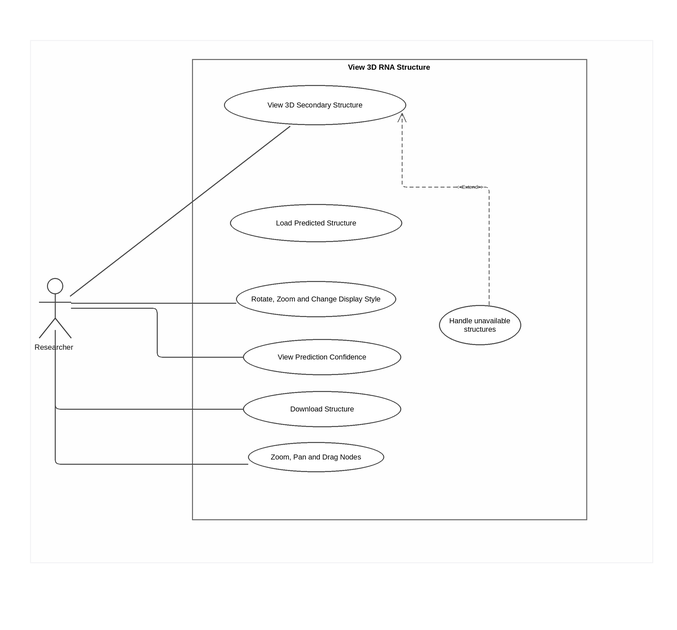
\includegraphics[width=0.8\textwidth]{Figures/UC_view_3d.png}
\caption[Use Case Diagram: View and Interact with 3D Structure]{Use Case Diagram: View and Interact with 3D Structure. Inside the View 3D RNA Structure system boundary, the Researcher is connected to View 3D Secondary Structure; Rotate, Zoom and Change Display Style; View Prediction Confidence; Download Structure; and Zoom, Pan and Drag Nodes. Load Predicted Structure is also shown, and Handle unavailable structures extends View 3D Secondary Structure.}
\label{fig:uc_view_3d}
\end{figure}

\begin{table}[H]
\centering
\caption{Use Case: View 2D Secondary Structure}
\label{tab:uc-2-5}
\setlength{\tabcolsep}{4pt}
\begin{tabular}{|lllll|}
\hline
\multicolumn{2}{|l|}{\textbf{Name}} &
  \multicolumn{3}{l|}{View 2D Secondary Structure} \\ \hline
\multicolumn{2}{|l|}{\textbf{Actors}} &
  \multicolumn{3}{l|}{Researcher} \\ \hline
\multicolumn{2}{|l|}{\textbf{Summary}} &
  \multicolumn{3}{l|}{\begin{tabular}[c]{@{}l@{}}The user shall view an interactive 2D graph of the secondary structure\\ (dot-bracket notation) used for the job. The structure is either\\ the dot-bracket provided by the user at submission or the one\\ predicted by the system, and its source is shown on the screen.\end{tabular}} \\ \hline
\multicolumn{2}{|l|}{\textbf{Pre-Conditions}} &
  \multicolumn{3}{l|}{\begin{tabular}[c]{@{}l@{}}The job must have finished successfully.\\ A dot-bracket structure must be available, either provided by the\\ user (already validated at submission) or generated by the system.\end{tabular}} \\ \hline
\multicolumn{2}{|l|}{\textbf{Post-Conditions}} &
  \multicolumn{3}{l|}{\begin{tabular}[c]{@{}l@{}}Success: The 2D graph, its dot-bracket string and its source label are\\ displayed on the screen.\\ Failure: No graph is displayed and an error message is shown.\end{tabular}} \\ \hline
\multicolumn{2}{|l|}{\textbf{\begin{tabular}[c]{@{}l@{}}Special\\ Requirements\end{tabular}}} &
  \multicolumn{3}{l|}{\begin{tabular}[c]{@{}l@{}}The graph shall be rendered as an interactive SVG supporting zoom\\ and pan.\end{tabular}} \\ \hline
\multicolumn{5}{|c|}{\textbf{Basic Flow}} \\ \hline
\multicolumn{3}{|c|}{\textbf{Actor Action}} &
  \multicolumn{2}{c|}{\textbf{System Response}} \\ \hline
\multicolumn{1}{|l|}{1} &
  \multicolumn{2}{l|}{\begin{tabular}[c]{@{}l@{}}The user opens the 2D\\ Structure screen.\end{tabular}} &
  \multicolumn{1}{l|}{2} &
  \begin{tabular}[c]{@{}l@{}}The system retrieves the dot-bracket structure and its\\ source, renders it as an interactive 2D graph, and labels it\\ as User-provided or Predicted (RNAfold).\end{tabular} \\ \hline
\multicolumn{1}{|l|}{3} &
  \multicolumn{2}{l|}{\begin{tabular}[c]{@{}l@{}}The user zooms, pans or\\ drags nodes in the graph.\end{tabular}} &
  \multicolumn{1}{l|}{4} &
  \begin{tabular}[c]{@{}l@{}}The system updates the graph accordingly.\end{tabular} \\ \hline
\multicolumn{5}{|c|}{\textbf{Alternative Flow}} \\ \hline
\multicolumn{1}{|l|}{1-A} &
  \multicolumn{2}{l|}{\begin{tabular}[c]{@{}l@{}}The user opens the 2D\\ Structure screen but no\\ structure is available.\end{tabular}} &
  \multicolumn{1}{l|}{2-A} &
  \begin{tabular}[c]{@{}l@{}}The system displays the error message: Secondary structure\\ could not be generated for this sequence. The use case ends.\end{tabular} \\ \hline
\multicolumn{1}{|l|}{1-B} &
  \multicolumn{2}{l|}{\begin{tabular}[c]{@{}l@{}}The user opens the 2D\\ Structure screen but the\\ stored dot-bracket string is\\ invalid or does not match\\ the sequence length.\end{tabular}} &
  \multicolumn{1}{l|}{2-B} &
  \begin{tabular}[c]{@{}l@{}}The system displays the error message: The secondary\\ structure could not be displayed because the dot-bracket\\ string is invalid. The use case ends.\end{tabular} \\ \hline
\end{tabular}
\end{table}

\begin{figure}[!htbp]
\centering
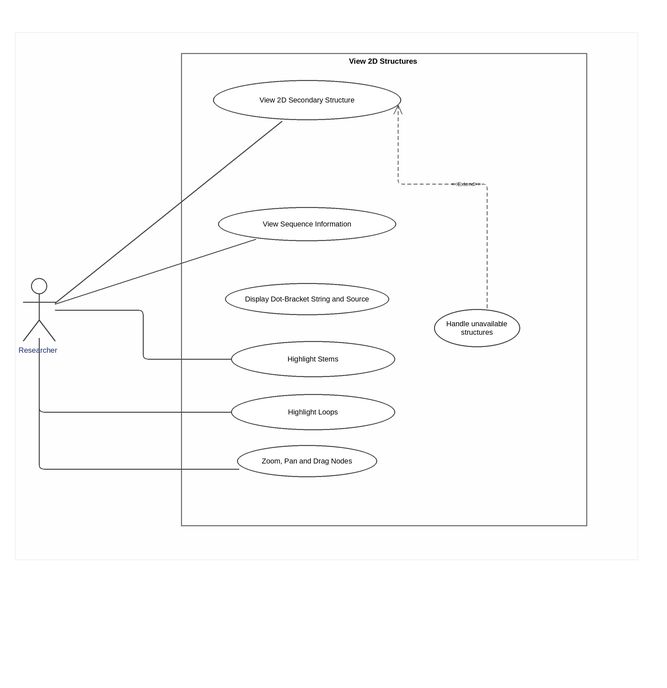
\includegraphics[width=0.8\textwidth]{Figures/UC_view_2d.png}
\caption[Use Case Diagram: View 2D Secondary Structure]{Use Case Diagram: View 2D Secondary Structure. Inside the View 2D Structures system boundary, the Researcher is connected to View 2D Secondary Structure, View Sequence Information, Highlight Stems, Highlight Loops, and Zoom, Pan and Drag Nodes. Display Dot-Bracket String and Source is also shown, and Handle unavailable structures extends View 2D Secondary Structure.}
\label{fig:uc_view_2d}
\end{figure}



\begin{table}[H]
\centering
\caption{Use Case: Sequence Input and Validation}
\label{tab:uc-sequence-input}
\begin{tabular}{|lllll|}
\hline
\multicolumn{2}{|l|}{\textbf{Name}} &
  \multicolumn{3}{l|}{Sequence Input and Validation} \\ \hline
\multicolumn{2}{|l|}{\textbf{Actors}} &
  \multicolumn{3}{l|}{Researcher} \\ \hline
\multicolumn{2}{|l|}{\textbf{Summary}} &
  \multicolumn{3}{l|}{\begin{tabular}[c]{@{}l@{}}The user enters or uploads an RNA sequence, optionally adds a 2D\\ structure in dot-bracket notation, and submits it. The system\\ validates the input before creating a prediction job.\end{tabular}} \\ \hline
\multicolumn{2}{|l|}{\textbf{Pre-Conditions}} &
  \multicolumn{3}{l|}{\begin{tabular}[c]{@{}l@{}}The user has an RNA sequence ready and has opened the sequence\\ input page.\end{tabular}} \\ \hline
\multicolumn{2}{|l|}{\textbf{Post-Conditions}} &
  \multicolumn{3}{l|}{\begin{tabular}[c]{@{}l@{}}The validated input is accepted, a prediction job is queued, and\\ the user is taken to the job status page.\end{tabular}} \\ \hline
\multicolumn{2}{|l|}{\textbf{\begin{tabular}[c]{@{}l@{}}Special\\ Requirements\end{tabular}}} &
  \multicolumn{3}{l|}{\begin{tabular}[c]{@{}l@{}}The sequence may contain only A, C, G, and U. The sequence must\\ be within the allowed length limit. If a dot-bracket is given, its\\ length must match the sequence length and its brackets must be\\ balanced. Error messages must be specific, e.g. ``Position 42\\ contains an invalid character.''\end{tabular}} \\ \hline
\multicolumn{5}{|c|}{\textbf{Basic Flow}} \\ \hline
\multicolumn{3}{|c|}{\textbf{Actor Action}} &
  \multicolumn{2}{c|}{\textbf{System Response}} \\ \hline
\multicolumn{1}{|l|}{1} &
  \multicolumn{2}{l|}{\begin{tabular}[c]{@{}l@{}}The user opens the\\ sequence input page.\end{tabular}} &
  \multicolumn{1}{l|}{2} &
  \begin{tabular}[c]{@{}l@{}}The system displays the input form with a sequence field,\\ a file upload option, and an optional dot-bracket field.\end{tabular} \\ \hline
\multicolumn{1}{|l|}{3} &
  \multicolumn{2}{l|}{\begin{tabular}[c]{@{}l@{}}The user pastes or\\ uploads an RNA sequence.\end{tabular}} &
  \multicolumn{1}{l|}{4} &
  \begin{tabular}[c]{@{}l@{}}The system reads the sequence and displays it in the form.\end{tabular} \\ \hline
\multicolumn{1}{|l|}{5} &
  \multicolumn{2}{l|}{\begin{tabular}[c]{@{}l@{}}The user optionally enters\\ a dot-bracket 2D structure.\end{tabular}} &
  \multicolumn{1}{l|}{6} &
  \begin{tabular}[c]{@{}l@{}}The system accepts the dot-bracket and displays it in the\\ form.\end{tabular} \\ \hline
\multicolumn{1}{|l|}{7} &
  \multicolumn{2}{l|}{\begin{tabular}[c]{@{}l@{}}The user clicks Submit.\end{tabular}} &
  \multicolumn{1}{l|}{8} &
  \begin{tabular}[c]{@{}l@{}}The system checks the valid characters, sequence length,\\ dot-bracket length, and bracket balance.\end{tabular} \\ \hline
\multicolumn{1}{|l|}{} &
  \multicolumn{2}{l|}{} &
  \multicolumn{1}{l|}{9} &
  \begin{tabular}[c]{@{}l@{}}The system creates a prediction job, adds it to the queue,\\ and redirects the user to the job status page.\end{tabular} \\ \hline
\multicolumn{5}{|c|}{\textbf{Alternative Flow}} \\ \hline
\multicolumn{1}{|l|}{7} &
  \multicolumn{2}{l|}{\begin{tabular}[c]{@{}l@{}}The user submits a\\ sequence or dot-bracket\\ that is invalid.\end{tabular}} &
  \multicolumn{1}{l|}{8-A} &
  \begin{tabular}[c]{@{}l@{}}The system displays a specific error message stating the\\ problem and its position, and keeps the user on the input\\ form.\end{tabular} \\ \hline
\multicolumn{1}{|l|}{3} &
  \multicolumn{2}{l|}{\begin{tabular}[c]{@{}l@{}}The user uploads a file\\ that cannot be read.\end{tabular}} &
  \multicolumn{1}{l|}{4-A} &
  \begin{tabular}[c]{@{}l@{}}The system displays an error message asking the user to\\ upload a valid sequence file.\end{tabular} \\ \hline
\end{tabular}
\end{table}

\begin{figure}[!htbp]
\centering
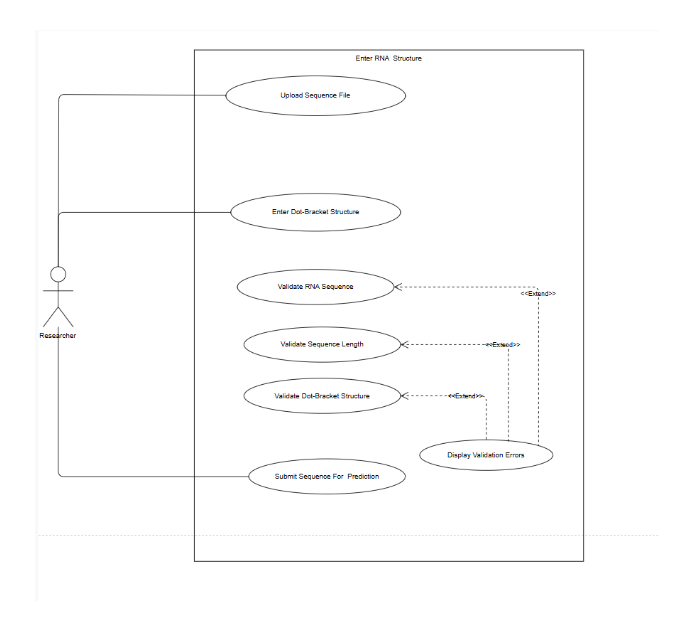
\includegraphics[width=0.8\textwidth]{Figures/UC_enter_rna_sequence.png}
\caption[Use Case Diagram: Sequence Input and Validation]{Use Case Diagram: Sequence Input and Validation. Inside the Enter RNA Structure system boundary, the Researcher is connected to Upload Sequence File, Enter Dot-Bracket Structure and Submit Sequence For Prediction. Display Validation Errors extends Validate RNA Sequence, Validate Sequence Length and Validate Dot-Bracket Structure.}
\label{fig:uc_enter_rna_sequence}
\end{figure}

\begin{table}[H]
\centering
\caption{Use Case: Job Status Tracking}
\label{tab:uc-job-status}
\begin{tabular}{|lllll|}
\hline
\multicolumn{2}{|l|}{\textbf{Name}} &
  \multicolumn{3}{l|}{Job Status Tracking} \\ \hline
\multicolumn{2}{|l|}{\textbf{Actors}} &
  \multicolumn{3}{l|}{Researcher} \\ \hline
\multicolumn{2}{|l|}{\textbf{Summary}} &
  \multicolumn{3}{l|}{\begin{tabular}[c]{@{}l@{}}The user views the state of a submitted job (queued, running,\\ finished, or failed) and the current pipeline stage. The user can\\ leave the page and return later to the result.\end{tabular}} \\ \hline
\multicolumn{2}{|l|}{\textbf{Pre-Conditions}} &
  \multicolumn{3}{l|}{The user has submitted a prediction job.} \\ \hline
\multicolumn{2}{|l|}{\textbf{Post-Conditions}} &
  \multicolumn{3}{l|}{\begin{tabular}[c]{@{}l@{}}The user sees the latest job state. A finished job gives access to\\ its results, and a failed job shows a failure message.\end{tabular}} \\ \hline
\multicolumn{2}{|l|}{\textbf{\begin{tabular}[c]{@{}l@{}}Special\\ Requirements\end{tabular}}} &
  \multicolumn{3}{l|}{\begin{tabular}[c]{@{}l@{}}Each job runs in the background. The job state and pipeline stage\\ must update without the user restarting the job. A failure must\\ show a clear message, e.g. ``Low confidence, no close template\\ found.''\end{tabular}} \\ \hline
\multicolumn{5}{|c|}{\textbf{Basic Flow}} \\ \hline
\multicolumn{3}{|c|}{\textbf{Actor Action}} &
  \multicolumn{2}{c|}{\textbf{System Response}} \\ \hline
\multicolumn{1}{|l|}{1} &
  \multicolumn{2}{l|}{\begin{tabular}[c]{@{}l@{}}The user opens the job\\ status page.\end{tabular}} &
  \multicolumn{1}{l|}{2} &
  \begin{tabular}[c]{@{}l@{}}The system displays the job state and the current pipeline\\ stage.\end{tabular} \\ \hline
\multicolumn{1}{|l|}{3} &
  \multicolumn{2}{l|}{\begin{tabular}[c]{@{}l@{}}The user leaves the page.\end{tabular}} &
  \multicolumn{1}{l|}{4} &
  \begin{tabular}[c]{@{}l@{}}The system continues running the job in the background.\end{tabular} \\ \hline
\multicolumn{1}{|l|}{5} &
  \multicolumn{2}{l|}{\begin{tabular}[c]{@{}l@{}}The user returns to the job\\ status page later.\end{tabular}} &
  \multicolumn{1}{l|}{6} &
  \begin{tabular}[c]{@{}l@{}}The system displays the latest job state and, if the job is\\ finished, a link to the results.\end{tabular} \\ \hline
\multicolumn{5}{|c|}{\textbf{Alternative Flow}} \\ \hline
\multicolumn{1}{|l|}{5} &
  \multicolumn{2}{l|}{\begin{tabular}[c]{@{}l@{}}The user returns to a job\\ that has failed or timed\\ out.\end{tabular}} &
  \multicolumn{1}{l|}{6-A} &
  \begin{tabular}[c]{@{}l@{}}The system displays a failure message explaining the reason\\ and offers the option to submit again.\end{tabular} \\ \hline
\end{tabular}
\end{table}

\begin{figure}[!htbp]
\centering
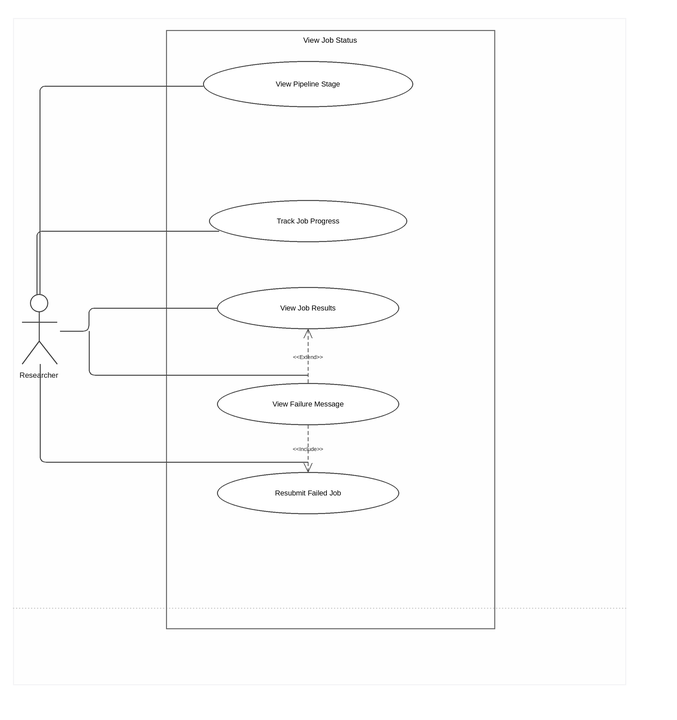
\includegraphics[width=0.8\textwidth]{Figures/UC_view_job_status.png}
\caption[Use Case Diagram: Job Status Tracking]{Use Case Diagram: Job Status Tracking. Inside the View Job Status system boundary, the Researcher is connected to View Pipeline Stage, Track Job Progress, View Job Results, View Failure Message and Resubmit Failed Job. View Failure Message extends View Job Results and includes Resubmit Failed Job.}
\label{fig:uc_view_job_status}
\end{figure}

\begin{table}[H]
\centering
\caption{Use Case: Run History}
\label{tab:uc-run-history}
\begin{tabular}{|lllll|}
\hline
\multicolumn{2}{|l|}{\textbf{Name}} &
  \multicolumn{3}{l|}{Run History} \\ \hline
\multicolumn{2}{|l|}{\textbf{Actors}} &
  \multicolumn{3}{l|}{Researcher} \\ \hline
\multicolumn{2}{|l|}{\textbf{Summary}} &
  \multicolumn{3}{l|}{\begin{tabular}[c]{@{}l@{}}The user views past jobs with their input, status, date, and\\ results. The user can reopen a past run, re-run it, or share a link\\ to it.\end{tabular}} \\ \hline
\multicolumn{2}{|l|}{\textbf{Pre-Conditions}} &
  \multicolumn{3}{l|}{The user has submitted at least one job before.} \\ \hline
\multicolumn{2}{|l|}{\textbf{Post-Conditions}} &
  \multicolumn{3}{l|}{\begin{tabular}[c]{@{}l@{}}The selected run is reopened, a new job is queued for a re-run,\\ or a shareable link is generated.\end{tabular}} \\ \hline
\multicolumn{2}{|l|}{\textbf{\begin{tabular}[c]{@{}l@{}}Special\\ Requirements\end{tabular}}} &
  \multicolumn{3}{l|}{\begin{tabular}[c]{@{}l@{}}Each run must have its own shareable link. Runs should be listed\\ with the newest first.\end{tabular}} \\ \hline
\multicolumn{5}{|c|}{\textbf{Basic Flow}} \\ \hline
\multicolumn{3}{|c|}{\textbf{Actor Action}} &
  \multicolumn{2}{c|}{\textbf{System Response}} \\ \hline
\multicolumn{1}{|l|}{1} &
  \multicolumn{2}{l|}{\begin{tabular}[c]{@{}l@{}}The user opens the run\\ history page.\end{tabular}} &
  \multicolumn{1}{l|}{2} &
  \begin{tabular}[c]{@{}l@{}}The system displays the list of past runs with input, status,\\ and date.\end{tabular} \\ \hline
\multicolumn{1}{|l|}{3} &
  \multicolumn{2}{l|}{\begin{tabular}[c]{@{}l@{}}The user selects a run and\\ chooses Reopen.\end{tabular}} &
  \multicolumn{1}{l|}{4} &
  \begin{tabular}[c]{@{}l@{}}The system loads the saved input and results of that run.\end{tabular} \\ \hline
\multicolumn{1}{|l|}{5} &
  \multicolumn{2}{l|}{\begin{tabular}[c]{@{}l@{}}The user chooses Re-run.\end{tabular}} &
  \multicolumn{1}{l|}{6} &
  \begin{tabular}[c]{@{}l@{}}The system creates a new job with the same input and adds\\ it to the queue.\end{tabular} \\ \hline
\multicolumn{1}{|l|}{7} &
  \multicolumn{2}{l|}{\begin{tabular}[c]{@{}l@{}}The user chooses Share.\end{tabular}} &
  \multicolumn{1}{l|}{8} &
  \begin{tabular}[c]{@{}l@{}}The system generates a link for that run and displays it to\\ copy.\end{tabular} \\ \hline
\multicolumn{5}{|c|}{\textbf{Alternative Flow}} \\ \hline
\multicolumn{1}{|l|}{1} &
  \multicolumn{2}{l|}{\begin{tabular}[c]{@{}l@{}}The user opens the run\\ history page with no\\ previous runs.\end{tabular}} &
  \multicolumn{1}{l|}{2-A} &
  \begin{tabular}[c]{@{}l@{}}The system displays a message that no runs exist yet and\\ links to the sequence input page.\end{tabular} \\ \hline
\end{tabular}
\end{table}

\begin{figure}[!htbp]
\centering
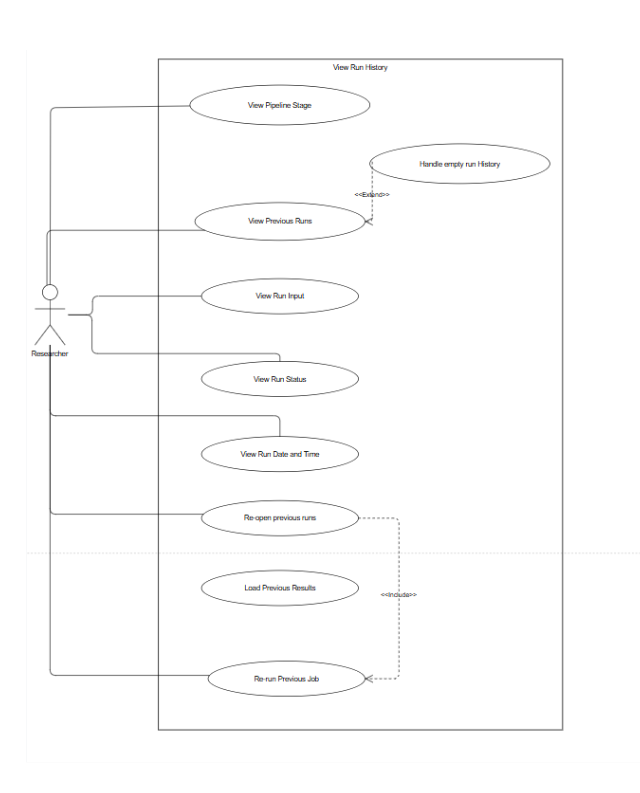
\includegraphics[width=0.8\textwidth]{Figures/UC_view_history.png}
\caption[Use Case Diagram: Run History]{Use Case Diagram: Run History. Inside the View Run History system boundary, the Researcher is connected to View Pipeline Stage, View Previous Runs, View Run Input, View Run Status, View Run Date and Time, Re-open previous runs and Re-run Previous Job. Handle empty run History extends View Previous Runs, Re-open previous runs includes Re-run Previous Job, and Load Previous Results is also shown.}
\label{fig:uc_view_history}
\end{figure}

\begin{table}[H]
\centering
\caption{Use Case: Chat with Structure}
\label{tab:uc-chat}
\setstretch{1.3}
\begin{tabular}{|lllll|}
\hline
\multicolumn{2}{|l|}{\textbf{Name}} &
  \multicolumn{3}{l|}{Chat with Structure} \\ \hline
\multicolumn{2}{|l|}{\textbf{Actors}} &
  \multicolumn{3}{l|}{Researcher} \\ \hline
\multicolumn{2}{|l|}{\textbf{Summary}} &
  \multicolumn{3}{l|}{\begin{tabular}[c]{@{}l@{}}The user asks natural-language questions about a predicted RNA\\ structure. The system gives the language model the structure's\\ metadata (sequence, length, GC content, dot-bracket, MFE,\\ detected pockets) and shows the model's answer.\end{tabular}} \\ \hline
\multicolumn{2}{|l|}{\textbf{Pre-Conditions}} &
  \multicolumn{3}{l|}{\begin{tabular}[c]{@{}l@{}}The prediction job for the structure has finished and its results\\ are available.\end{tabular}} \\ \hline
\multicolumn{2}{|l|}{\textbf{Post-Conditions}} &
  \multicolumn{3}{l|}{\begin{tabular}[c]{@{}l@{}}The user's question and the model's answer are shown in the chat\\ and saved in the chat history of that job.\end{tabular}} \\ \hline
\multicolumn{2}{|l|}{\textbf{\begin{tabular}[c]{@{}l@{}}Special\\ Requirements\end{tabular}}} &
  \multicolumn{3}{l|}{\begin{tabular}[c]{@{}l@{}}The metadata must be extracted after the 3D prediction finishes\\ and passed to the language model as context. The answer must\\ be shown in the chat window. Empty questions must not be sent.\end{tabular}} \\ \hline
\multicolumn{5}{|c|}{\textbf{Basic Flow}} \\ \hline
\multicolumn{3}{|c|}{\textbf{Actor Action}} &
  \multicolumn{2}{c|}{\textbf{System Response}} \\ \hline
\multicolumn{1}{|l|}{1} &
  \multicolumn{2}{l|}{\begin{tabular}[c]{@{}l@{}}The user opens the chat\\ for a predicted structure.\end{tabular}} &
  \multicolumn{1}{l|}{2} &
  \begin{tabular}[c]{@{}l@{}}The system checks that the job has finished and displays the\\ chat window with suggested questions.\end{tabular} \\ \hline
\multicolumn{1}{|l|}{3} &
  \multicolumn{2}{l|}{\begin{tabular}[c]{@{}l@{}}The user types a question\\ about the structure, or\\ selects a suggested\\ question.\end{tabular}} &
  \multicolumn{1}{l|}{4} &
  \begin{tabular}[c]{@{}l@{}}The system extracts the structure metadata and builds the\\ context prompt.\end{tabular} \\ \hline
\multicolumn{1}{|l|}{} &
  \multicolumn{2}{l|}{} &
  \multicolumn{1}{l|}{5} &
  \begin{tabular}[c]{@{}l@{}}The system sends the prompt and the question to the\\ language model.\end{tabular} \\ \hline
\multicolumn{1}{|l|}{6} &
  \multicolumn{2}{l|}{\begin{tabular}[c]{@{}l@{}}The user reads the\\ response.\end{tabular}} &
  \multicolumn{1}{l|}{7} &
  \begin{tabular}[c]{@{}l@{}}The system displays the language model's response in the\\ chat.\end{tabular} \\ \hline
\multicolumn{5}{|c|}{\textbf{Alternative Flow}} \\ \hline
\multicolumn{1}{|l|}{1} &
  \multicolumn{2}{l|}{\begin{tabular}[c]{@{}l@{}}The user opens the chat\\ for a job that has not\\ finished or has failed.\end{tabular}} &
  \multicolumn{1}{l|}{2-A} &
  \begin{tabular}[c]{@{}l@{}}The system displays a message that chat is unavailable until\\ the job finishes successfully.\end{tabular} \\ \hline
\multicolumn{1}{|l|}{3} &
  \multicolumn{2}{l|}{\begin{tabular}[c]{@{}l@{}}The user submits an\\ empty question.\end{tabular}} &
  \multicolumn{1}{l|}{4-A} &
  \begin{tabular}[c]{@{}l@{}}The system asks the user to enter a question and does not\\ send it.\end{tabular} \\ \hline
\multicolumn{1}{|l|}{5} &
  \multicolumn{2}{l|}{\begin{tabular}[c]{@{}l@{}}The language model fails\\ or times out.\end{tabular}} &
  \multicolumn{1}{l|}{6-A} &
  \begin{tabular}[c]{@{}l@{}}The system displays an error message and lets the user try\\ the question again.\end{tabular} \\ \hline
\multicolumn{1}{|l|}{1} &
  \multicolumn{2}{l|}{\begin{tabular}[c]{@{}l@{}}The user chooses to view\\ earlier messages or clear\\ the conversation.\end{tabular}} &
  \multicolumn{1}{l|}{2-B} &
  \begin{tabular}[c]{@{}l@{}}The system displays the saved chat history for the job, or\\ clears it when the user confirms.\end{tabular} \\ \hline
\end{tabular}
\end{table}

\begin{figure}[!htbp]
\centering
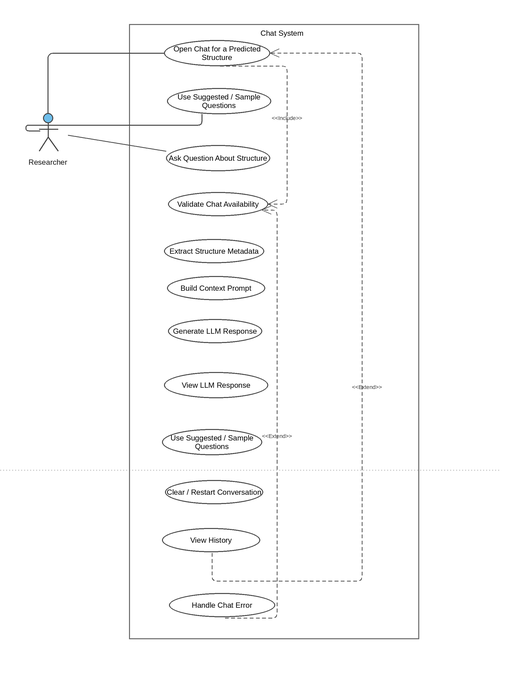
\includegraphics[width=0.8\textwidth]{Figures/UC_chat.png}
\caption[Use Case Diagram: Chat with Structure]{Use Case Diagram: Chat with Structure. Inside the Chat System boundary, the Researcher is connected to Open Chat for a Predicted Structure, Use Suggested / Sample Questions and Ask Question About Structure. The system's steps are Validate Chat Availability, Extract Structure Metadata, Build Context Prompt, Generate LLM Response and View LLM Response, with Clear / Restart Conversation, View History and Handle Chat Error linked to them by include and extend relationships.}
\label{fig:uc_chat}
\end{figure}

\section{Hardware and Software Requirements}
The requirements below cover developing and running the experiments in Chapter~\ref{ch:approach}, and running the web application for development and demonstration.

\subsection{Hardware Requirements}
The hardware below is needed to run the pipeline and train the models.
\begin{itemize}
    \item GPUs. RNAPro needs high-memory GPUs for inference, and also for training or fine-tuning if we do a full retrain. Because of the model's large memory needs, the original RNAPro work used eight GB300 GPUs. We will use the closest setup available to us.
    \item CPU and memory. Enough CPU cores and system memory to run the template search methods, build features, and compute TM-align labels for every candidate template in the training and validation splits.
    \item Storage. Enough disk space for:
    \begin{itemize}
    \item the PDB structures with C1$'$ coordinates;
    \item the MSAs;
    \item the Eigen dataset;
    \item the candidate templates and their stored labels;
    \item the model checkpoints.
    \end{itemize}
\end{itemize}

\subsection{Software Requirements}
The software below is needed to build and run the pipeline and the web application.
\begin{itemize}
    \item Prediction model. RNAPro~\cite{leerna}, which is built on Protenix (a reproduction of AlphaFold~3), along with the Protenix base checkpoints we use for initialization.
    \item Template search tools. MMseqs2 and Infernal with Rfam, plus tools for embedding-based and secondary-structure-aware search. For the secondary-structure-aware search we are considering BEAGLE, but this is not confirmed yet.
    \item MSA generation. The rMSA pipeline. We convert T to U in its outputs.
    \item Structure scoring. US-align, run on the C1$'$ atom with sequence-independent alignment. We use it for the TM-align labels, for model evaluation and for comparing templates to find near-duplicates.
    \item RNA language models. RNet2 as the default and AIDO.RNA. We will choose other models later for the language-model comparison.
    \item Data. PDB structures, the Eigen dataset (up-to-date sequences and MSAs) and a structural-similarity benchmark for template-poor targets. We plan to use RNA3DB for the benchmark.
    \item Selector model. A ranking or regression model, along with the software to train and tune it. We haven't fixed the model type yet.
    \item Web front end. React 18 with TypeScript, built with Vite on Node.js and its npm package manager. The 3D viewer is Mol* (the molstar package), and the 2D secondary-structure diagram uses fornac.
    \item Web back end. FastAPI with Pydantic for request validation, served by Uvicorn. It exposes a REST API to the front end.
    \item Database. PostgreSQL 16, accessed through SQLAlchemy, with Alembic for schema migrations.
    \item Job queue. Celery with a Redis broker, with separate CPU and GPU worker queues, so that long-running predictions run in the background.
    \item Secondary structure and thermodynamics. ViennaRNA (RNAfold) predicts dot-bracket structures and minimum free energies for the 2D view and the chat metadata.
    \item Chat assistant. A hosted large language model accessed through its API, given the predicted structure's metadata as context.
    \item Deployment. Docker Compose packages the front end, back end, database, queue and workers for the demonstration.
\end{itemize}

\section{Graphical User Interface}
This section shows the main screens of the web application:
\begin{itemize}
\item sequence input (Figure~\ref{fig:InputValidation});
\item job status (Figure~\ref{fig:job-status});
\item the 2D structure view and its element details (Figures~\ref{fig:view-2D} and~\ref{fig:extended-2D});
\item the 3D structure view (Figure~\ref{fig:view-3d});
\item the ranked candidate list (Figure~\ref{fig:candidates});
\item the run history (Figure~\ref{fig:history});
\item the prediction information page (Figure~\ref{fig:prediction-info});
\item the chatbot (Figure~\ref{fig:chatbot}).
\end{itemize}

Each screen covers one use case of Section~\ref{sec:usecases}. The sequence input screen covers Sequence Input and Validation (Table~\ref{tab:uc-sequence-input}), the job status screen covers Job Status Tracking (Table~\ref{tab:uc-job-status}), the 2D view and its details panel cover View 2D Secondary Structure (Table~\ref{tab:uc-2-5}), the 3D view and the ranked candidate list cover View and Interact with 3D Structure (Table~\ref{tab:uc-2-1}), the history screen covers Run History (Table~\ref{tab:uc-run-history}) and the chatbot covers Chat with Structure (Table~\ref{tab:uc-chat}). The prediction information page is the methodology page of FR-19.

Every user follows the same navigation flow. A user starts on the sequence input screen and, after a valid submission, is taken to the job status screen. When the job finishes, the status screen links to the results, where the 3D view, the ranked candidate list and the 2D view can be opened, and the chatbot can be started for the selected prediction. The history screen lists earlier runs and reopens any of them at its results.

\begin{figure}[!htbp]
    \centering
    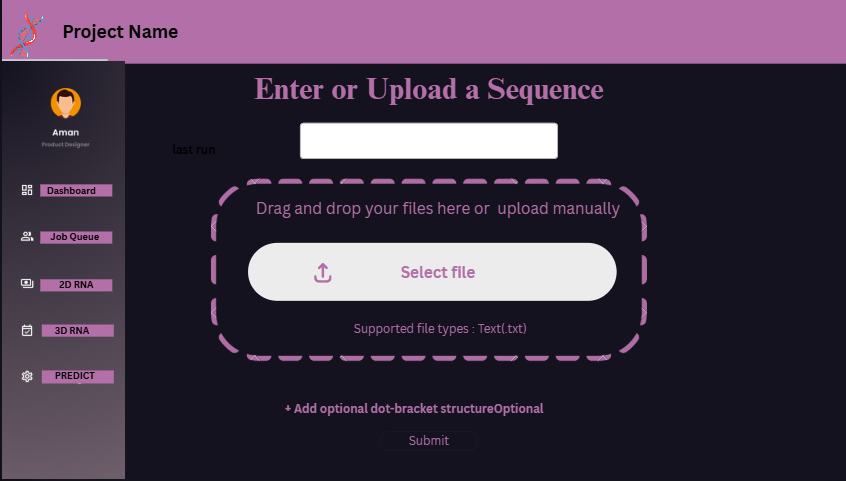
\includegraphics[width=0.7\textwidth]{gui/screen_5.png}
    \caption{Sequence Input and Validation screen}
    \label{fig:InputValidation}
\end{figure}

\begin{figure}[!htbp]
    \centering
    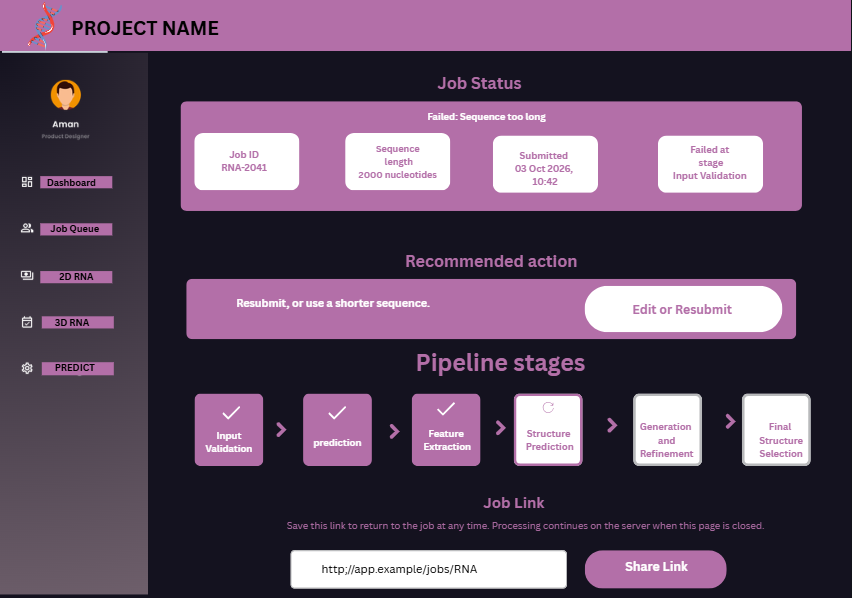
\includegraphics[width=0.7\textwidth]{gui/screen_6.png}
    \caption{Job Status Tracking screen, showing a failed job, the recommended action and the pipeline stages}
    \label{fig:job-status}
\end{figure}

\begin{figure}[!htbp]
    \centering
    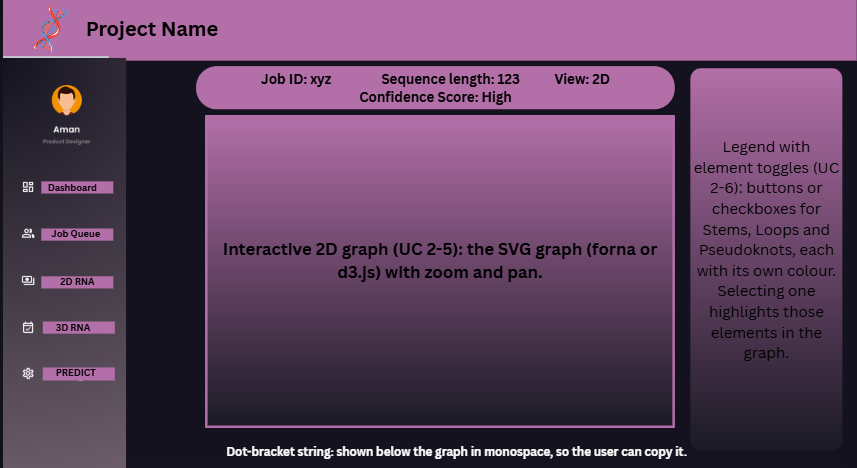
\includegraphics[width=0.7\textwidth]{gui/screen_3.png}
    \caption{View 2D Secondary Structure screen, with the legend and element toggles}
    \label{fig:view-2D}
\end{figure}

\begin{figure}[!htbp]
    \centering
    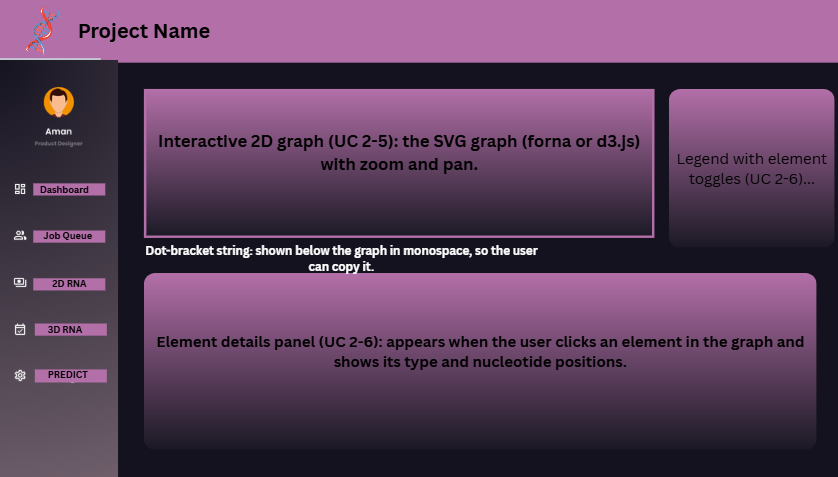
\includegraphics[width=0.7\textwidth]{gui/screen_4.png}
    \caption{2D view with the element details panel for stems, loops and pseudoknots}
    \label{fig:extended-2D}
\end{figure}

\begin{figure}[!htbp]
    \centering
    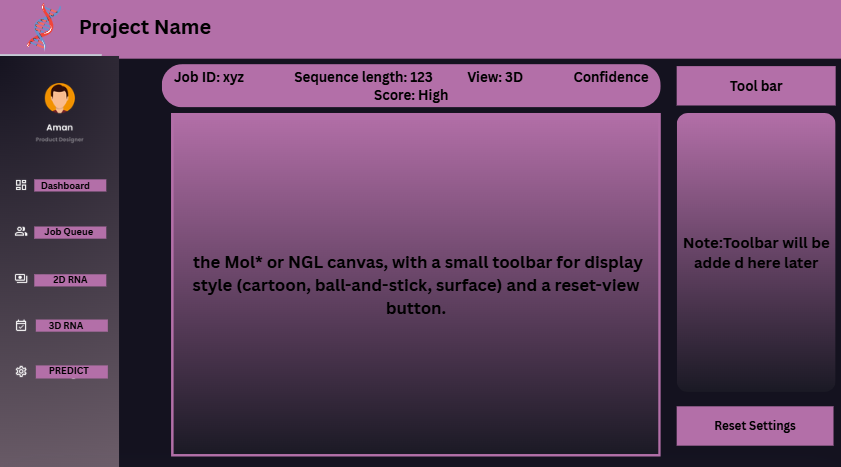
\includegraphics[width=0.7\textwidth]{gui/screen_1.png}
    \caption{View and Interact with 3D Structure screen}
    \label{fig:view-3d}
\end{figure}

\begin{figure}[!htbp]
    \centering
    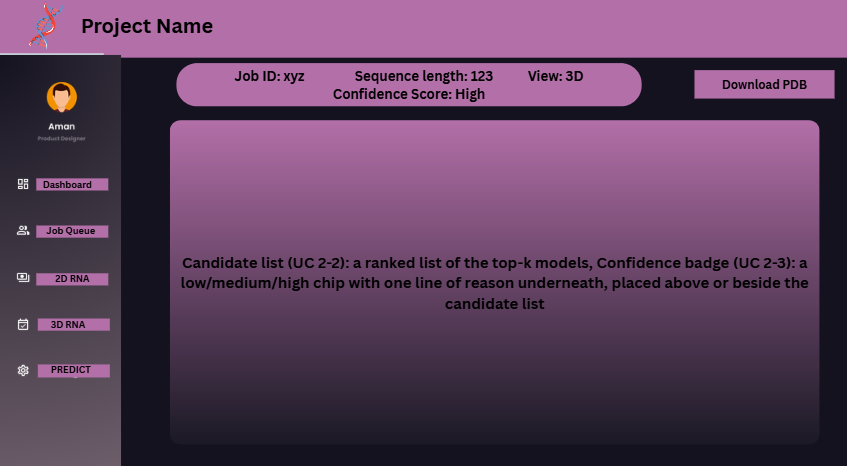
\includegraphics[width=0.7\textwidth]{gui/screen_2.png}
    \caption{Ranked candidate list with confidence badge and PDB download}
    \label{fig:candidates}
\end{figure}

\begin{figure}[!htbp]
    \centering
    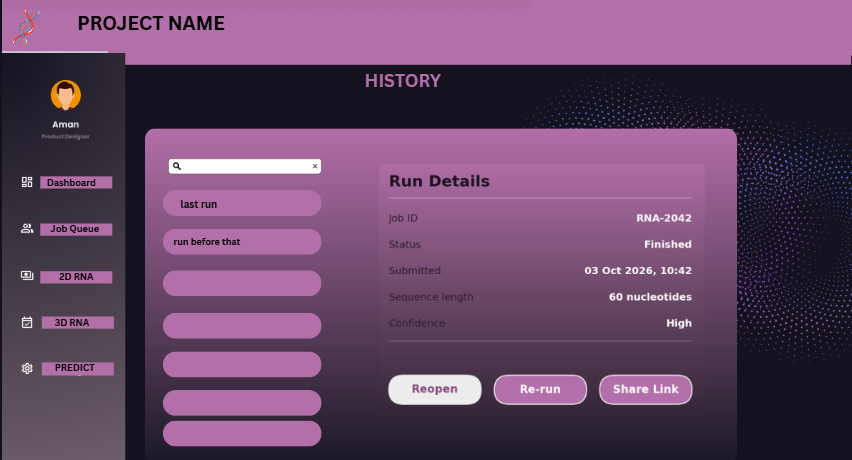
\includegraphics[width=0.7\textwidth]{gui/screen_7.png}
    \caption{History screen listing previous runs, with run details and the Reopen, Re-run and Share Link actions}
    \label{fig:history}
\end{figure}

\begin{figure}[!htbp]
    \centering
    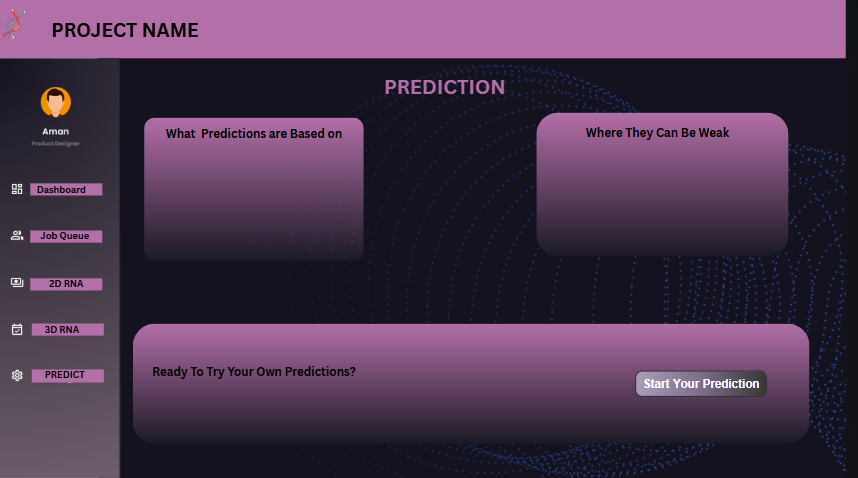
\includegraphics[width=0.7\textwidth]{gui/screen_8.png}
    \caption{Prediction information page describing what predictions are based on and where they can be weak}
    \label{fig:prediction-info}
\end{figure}

\begin{figure}[!htbp]
    \centering
    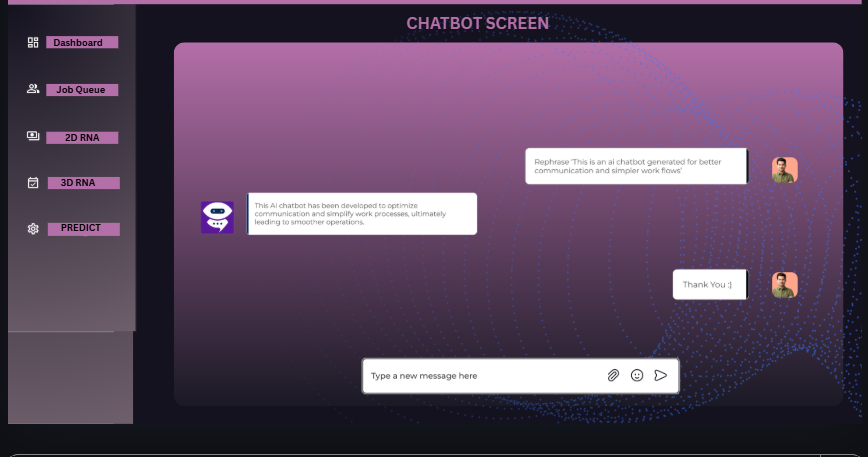
\includegraphics[width=0.7\textwidth]{gui/screen_9.png}
    \caption{Chatbot screen for asking questions about a predicted structure}
    \label{fig:chatbot}
\end{figure}
\section{Database Design}
This section describes the database design of the web application: the entity-relationship diagram and the data dictionary.

\subsection{ER Diagram}
Figure~\ref{fig:ERD} shows the entity-relationship diagram of the system. The data dictionary that follows describes each table.

\begin{figure}[!htbp]
    \centering
    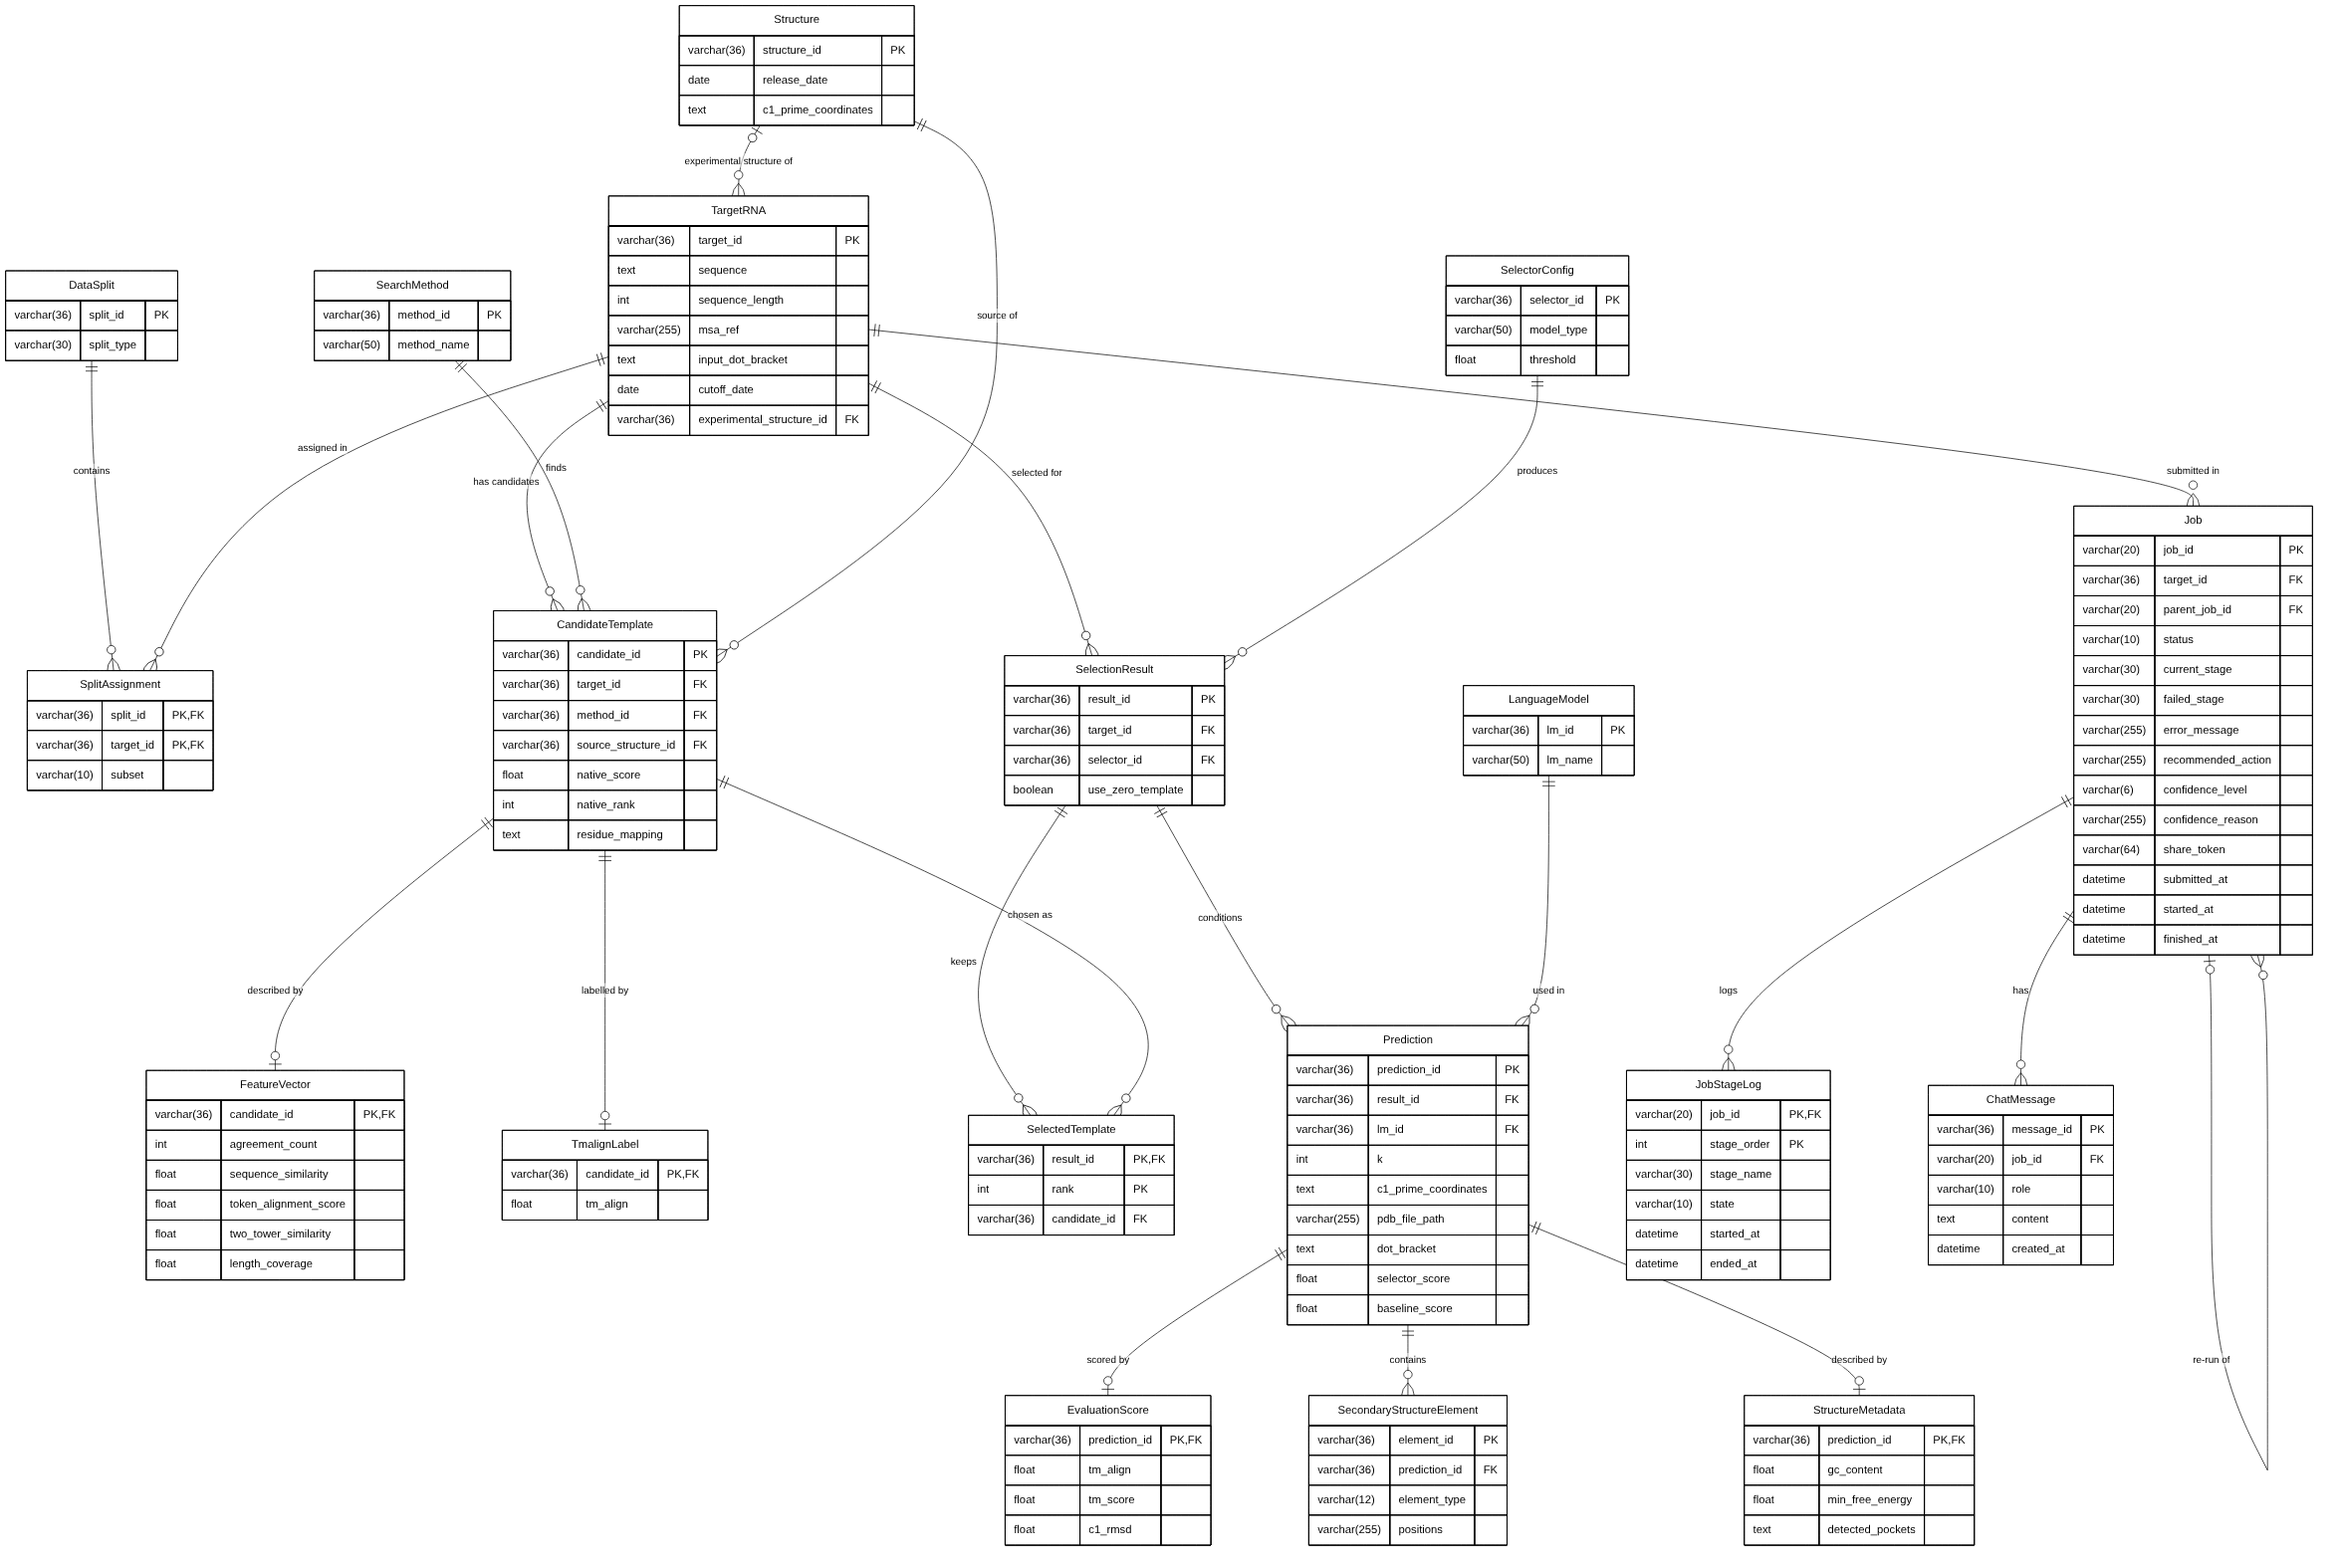
\includegraphics[width=0.7\textwidth]{Figures/ERD.png}
    \caption[Proposed ERD]{Proposed ERD. It shows the 19 entities of the database (TargetRNA, Structure, DataSplit, SplitAssignment, SearchMethod, CandidateTemplate, FeatureVector, TmalignLabel, SelectorConfig, SelectionResult, SelectedTemplate, LanguageModel, Prediction, EvaluationScore, SecondaryStructureElement, StructureMetadata, Job, JobStageLog and ChatMessage), each with its columns, data types and primary and foreign keys, and the relationships between them.}
    \label{fig:ERD}
\end{figure}

\subsection{Data Dictionary}
Following is the Data Dictionary for the RNA structure prediction system:

\tbl{TargetRNA}{A table describing attributes and their descriptions for a target RNA submitted for prediction}{
\rw{target\_id}{varchar(36)}{Identifier for the target RNA}{No}{Yes}{PK}
\rw{sequence}{text}{RNA sequence (A, C, G, U)}{No}{No}{-}
\rw{sequence\_length}{int}{Number of nucleotides in the sequence}{No}{No}{-}
\rw{msa\_ref}{varchar(255)}{Reference to the multiple sequence alignment}{Yes}{No}{-}
\rw{input\_dot\_bracket}{text}{Optional dot-bracket secondary structure supplied by the user}{Yes}{No}{-}
\rw{cutoff\_date}{date}{Date after which structures are excluded as templates}{Yes}{No}{-}
\rw{experimental\_structure\_id}{varchar(36)}{Known experimental structure of the target, if any}{Yes}{No}{FK}
}

\tbl{Structure}{A table describing attributes and their descriptions for a known 3D structure}{
\rw{structure\_id}{varchar(36)}{Identifier for the structure}{No}{Yes}{PK}
\rw{release\_date}{date}{Date the structure was released}{No}{No}{-}
\rw{c1\_prime\_coordinates}{text}{C1' atom coordinates (JSON array)}{No}{No}{-}
}

\tbl{DataSplit}{A table describing attributes and their descriptions for a data split definition}{
\rw{split\_id}{varchar(36)}{Identifier for the split}{No}{Yes}{PK}
\rw{split\_type}{varchar(30)}{Type of split (e.g. temporal, family)}{No}{No}{-}
}

\tbl{SplitAssignment}{A table describing attributes and their descriptions for the assignment of targets to splits}{
\rw{split\_id}{varchar(36)}{Split the target belongs to}{No}{No}{PK, FK}
\rw{target\_id}{varchar(36)}{Target assigned to the split}{No}{No}{PK, FK}
\rw{subset}{varchar(10)}{Subset of the split: train, val or test}{No}{No}{-}
}

\tbl{SearchMethod}{A table describing attributes and their descriptions for a template retrieval method}{
\rw{method\_id}{varchar(36)}{Identifier for the retrieval method}{No}{Yes}{PK}
\rw{method\_name}{varchar(50)}{Name of the method (e.g. structural-token, two-tower, MMseqs2 baseline)}{No}{Yes}{-}
}

\tbl{CandidateTemplate}{A table describing attributes and their descriptions for a candidate template found for a target}{
\rw{candidate\_id}{varchar(36)}{Identifier for the candidate}{No}{Yes}{PK}
\rw{target\_id}{varchar(36)}{Target the candidate was found for}{No}{No}{FK}
\rw{method\_id}{varchar(36)}{Method that found the candidate}{No}{No}{FK}
\rw{source\_structure\_id}{varchar(36)}{Structure the template comes from}{No}{No}{FK}
\rw{native\_score}{float}{Score given by the retrieval method}{No}{No}{-}
\rw{native\_rank}{int}{Rank given by the retrieval method}{No}{No}{-}
\rw{residue\_mapping}{text}{Mapping of target residues to template residues (JSON)}{Yes}{No}{-}
}

\tbl{FeatureVector}{A table describing attributes and their descriptions for the features of a candidate template}{
\rw{candidate\_id}{varchar(36)}{Candidate the features describe}{No}{Yes}{PK, FK}
\rw{agreement\_count}{int}{Number of methods that found this template}{No}{No}{-}
\rw{sequence\_similarity}{float}{Sequence similarity to the target (0--1)}{No}{No}{-}
\rw{token\_alignment\_score}{float}{Alignment score between predicted and template structural tokens}{Yes}{No}{-}
\rw{two\_tower\_similarity}{float}{Similarity of the target and template in the two-tower space}{Yes}{No}{-}
\rw{length\_coverage}{float}{Fraction of the target covered by the alignment}{No}{No}{-}
}

\tbl{TmalignLabel}{A table describing attributes and their descriptions for a training label of a candidate}{
\rw{candidate\_id}{varchar(36)}{Candidate being labelled}{No}{Yes}{PK, FK}
\rw{tm\_align}{float}{TM-align score against the experimental structure}{No}{No}{-}
}

\tbl{SelectorConfig}{A table describing attributes and their descriptions for a template selector configuration}{
\rw{selector\_id}{varchar(36)}{Identifier for the configuration}{No}{Yes}{PK}
\rw{model\_type}{varchar(50)}{Type of selector model}{No}{No}{-}
\rw{threshold}{float}{Score threshold for using templates (0--1)}{No}{No}{-}
}

\tbl{SelectionResult}{A table describing attributes and their descriptions for the outcome of template selection}{
\rw{result\_id}{varchar(36)}{Identifier for the selection result}{No}{Yes}{PK}
\rw{target\_id}{varchar(36)}{Target the result belongs to}{No}{No}{FK}
\rw{selector\_id}{varchar(36)}{Selector configuration used}{No}{No}{FK}
\rw{use\_zero\_template}{boolean}{True if prediction should run without a template}{No}{No}{-}
}

\tbl{SelectedTemplate}{A table describing attributes and their descriptions for templates kept by a selection result}{
\rw{result\_id}{varchar(36)}{Selection result the template belongs to}{No}{No}{PK, FK}
\rw{rank}{int}{Position of the template in the selected order}{No}{No}{PK}
\rw{candidate\_id}{varchar(36)}{Candidate chosen}{No}{No}{FK}
}

\tbl{LanguageModel}{A table describing attributes and their descriptions for a language model}{
\rw{lm\_id}{varchar(36)}{Identifier for the language model}{No}{Yes}{PK}
\rw{lm\_name}{varchar(50)}{Name of the model (e.g. RNet2, AIDORNA)}{No}{Yes}{-}
}

\tbl{Prediction}{A table describing attributes and their descriptions for a predicted structure}{
\rw{prediction\_id}{varchar(36)}{Identifier for the prediction}{No}{Yes}{PK}
\rw{result\_id}{varchar(36)}{Selection result used}{No}{No}{FK}
\rw{lm\_id}{varchar(36)}{Language model used}{No}{No}{FK}
\rw{k}{int}{Rank of the model among the top-k (1--5)}{No}{No}{-}
\rw{c1\_prime\_coordinates}{text}{Predicted C1' coordinates (JSON array)}{No}{No}{-}
\rw{pdb\_file\_path}{varchar(255)}{Path to the PDB file offered for download}{Yes}{No}{-}
\rw{dot\_bracket}{text}{Dot-bracket string shown under the 2D graph}{Yes}{No}{-}
\rw{selector\_score}{float}{Score from the selector}{Yes}{No}{-}
\rw{baseline\_score}{float}{Baseline score for comparison}{Yes}{No}{-}
}

\tbl{EvaluationScore}{A table describing attributes and their descriptions for the evaluation of a prediction}{
\rw{prediction\_id}{varchar(36)}{Prediction being scored}{No}{Yes}{PK, FK}
\rw{tm\_align}{float}{TM-align result}{No}{No}{-}
\rw{tm\_score}{float}{TM-score (0--1)}{No}{No}{-}
\rw{c1\_rmsd}{float}{C1' root-mean-square deviation}{No}{No}{-}
}

\tbl{Job}{A table describing attributes and their descriptions for a prediction job and its status}{
\rw{job\_id}{varchar(20)}{Identifier shown to the user (e.g. RNA-2041)}{No}{Yes}{PK}
\rw{target\_id}{varchar(36)}{Target RNA submitted in the job}{No}{No}{FK}
\rw{parent\_job\_id}{varchar(20)}{Job this one re-runs, if any}{Yes}{No}{FK}
\rw{status}{varchar(10)}{queued, running, finished or failed}{No}{No}{-}
\rw{current\_stage}{varchar(30)}{Pipeline stage currently running}{Yes}{No}{-}
\rw{failed\_stage}{varchar(30)}{Stage at which the job failed}{Yes}{No}{-}
\rw{error\_message}{varchar(255)}{Reason for failure (e.g. sequence too long)}{Yes}{No}{-}
\rw{recommended\_action}{varchar(255)}{Advice shown on failure}{Yes}{No}{-}
\rw{confidence\_level}{varchar(6)}{low, medium or high}{Yes}{No}{-}
\rw{confidence\_reason}{varchar(255)}{One-line reason for the confidence level}{Yes}{No}{-}
\rw{share\_token}{varchar(64)}{Token used in the shareable job link}{No}{Yes}{-}
\rw{submitted\_at}{datetime}{Time the job was submitted}{No}{No}{-}
\rw{started\_at}{datetime}{Time processing began}{Yes}{No}{-}
\rw{finished\_at}{datetime}{Time the job finished or failed}{Yes}{No}{-}
}

\tbl{JobStageLog}{A table describing attributes and their descriptions for the progress of a job through pipeline stages}{
\rw{job\_id}{varchar(20)}{Job the stage belongs to}{No}{No}{PK, FK}
\rw{stage\_order}{int}{Position of the stage in the pipeline (1--6)}{No}{No}{PK}
\rw{stage\_name}{varchar(30)}{Name of the stage}{No}{No}{-}
\rw{state}{varchar(10)}{pending, running, done or failed}{No}{No}{-}
\rw{started\_at}{datetime}{Time the stage began}{Yes}{No}{-}
\rw{ended\_at}{datetime}{Time the stage ended}{Yes}{No}{-}
}

\tbl{SecondaryStructureElement}{A table describing attributes and their descriptions for stems, loops and pseudoknots of a prediction}{
\rw{element\_id}{varchar(36)}{Identifier for the element}{No}{Yes}{PK}
\rw{prediction\_id}{varchar(36)}{Prediction the element belongs to}{No}{No}{FK}
\rw{element\_type}{varchar(12)}{stem, loop or pseudoknot}{No}{No}{-}
\rw{positions}{varchar(255)}{Nucleotide positions of the element}{No}{No}{-}
}

\tbl{StructureMetadata}{A table describing attributes and their descriptions for metadata used as chat context}{
\rw{prediction\_id}{varchar(36)}{Prediction the metadata describes}{No}{Yes}{PK, FK}
\rw{gc\_content}{float}{Fraction of G and C nucleotides (0--1)}{No}{No}{-}
\rw{min\_free\_energy}{float}{Minimum free energy (kcal/mol)}{Yes}{No}{-}
\rw{detected\_pockets}{text}{Detected binding pockets}{Yes}{No}{-}
}

\tbl{ChatMessage}{A table describing attributes and their descriptions for chat messages about a prediction}{
\rw{message\_id}{varchar(36)}{Identifier for the message}{No}{Yes}{PK}
\rw{job\_id}{varchar(20)}{Job the conversation belongs to}{No}{No}{FK}
\rw{role}{varchar(10)}{user or assistant}{No}{No}{-}
\rw{content}{text}{Message text}{No}{No}{-}
\rw{created\_at}{datetime}{Time the message was sent}{No}{No}{-}
}

\section{Risk Analysis}
This section lists the risks that could affect the project and how we plan to reduce each one. We group them into four areas: technical, data and evaluation, schedule and resource, and project risks. The likelihood and impact judgements are our own initial estimates, and we will revisit them as the work progresses.

\subsection{Technical Risks}
The most serious technical risk is that we cannot reproduce the baseline. The RNAPro study trained on eight GB300 GPUs and does not report every hyperparameter. To deal with this, we will:
\begin{itemize}
\item use the authors' public release and checkpoints where they are available;
\item report every choice we make ourselves;
\item if full retraining is not feasible, use the best alternative we can run and say so clearly.
\end{itemize}

The second risk is that the learned selector does not beat simple baselines, such as naive pooling or the first-place Kaggle search. We will start with a simple model, add complexity only if validation results justify it, and report a negative result honestly if that is what we get.

There is also a related problem. Accuracy is capped by the best template in the pool. On top of that, the backbone may work better with the kind of templates it saw in training than with the ones our selector picks. We will report how close the selector gets to the best-template upper bound and state this mismatch as a limitation.

The third risk concerns the language models. An alternative model such as AIDO.RNA may not give the pair-level outputs that RNAPro expects from RNet2. We will check compatibility before training. If needed, we will derive pair features inside the adapter and report this as our own design decision.

Search tools may also fail or return nothing for some targets. We treat this as a normal case rather than an error: the pool uses whatever the other sources return, falls back to the zero-valued template if it ends up empty, and logs the failure.

Very long sequences are a separate problem. They may exceed the training crop size of 512 or run out of memory. For these, we will:
\begin{itemize}
\item set a length limit in input validation;
\item show the user a clear message;
\item report long sequences separately.
\end{itemize}

Finally, putting several search tools, a 48-block model and a web application together increases the chance of version and dependency conflicts. We will fix and record software versions, keep components behind shared interfaces, and test each one on its own.

\subsection{Data and Evaluation Risks}
Data leakage is the most important evaluation risk. If a search or training step sees a structure released after the target's cutoff, our results will look better than they really are. We enforce the split inside the structure repository, so every read is filtered by the target. We also add a test that checks that no structure released after a cutoff is ever returned.

The test set is small. The RNAPro study had only ten RNA-Puzzles targets, which limits statistical power. Where we can, we will report confidence intervals or significance tests, and we will avoid strong claims based on small differences.

Results may also not generalise to template-poor RNAs, since about 95\% of the competition's final targets had a usable template. We will add a structural-similarity benchmark (RNA3DB is planned) and report template-poor targets separately.

The RNAPro results are retrospective, and we have no access to a prospective blind test. We state this as a threat to validity and do not claim prospective accuracy.

Computing TM-align labels for every candidate is expensive, and the labels are sensitive to alignment settings. We compute them once, store them together with the software versions and settings, and reuse them.

Last, some datasets (the Eigen data, the MSAs, RNA3DB) may turn out to be unavailable or hard to process in time. We will confirm availability early. If needed, we will fall back to data we can access and document the change.

\subsection{Schedule and Resource Risks}
We are likely to be limited on GPU time and storage, because training, caching candidates and running predictions all need substantial compute. To make the most of what we have, we will precompute and cache labels and features, use published checkpoints, and prioritise the experiments that answer our main research question.

The scope is also large. It covers a research pipeline, a language-model comparison and a web application with many features. We will build in priority order:
\begin{enumerate}
\item baseline;
\item candidate generation;
\item selector;
\item web application.
\end{enumerate}
Optional features such as the chat assistant and the 2D viewer have lower priority.

Prediction jobs are compute-heavy, and the queue may grow when several users submit at once. This is why predictions run as background jobs with visible stages, and why we target only a small demonstration load.

Illness, other coursework or hardware failure could also delay the work. We will hold regular supervisor meetings, use version control and backups, and leave slack in the FYP-II plan.

\subsection{Project and Business Risks}
Users may trust predictions too much, for example by treating a low-confidence model as reliable. We reduce this risk in three ways:
\begin{itemize}
\item a confidence indicator that gives a reason;
\item a methodology page that explains the method's limits;
\item a rule that the system does not show a poor result silently.
\end{itemize}

A privacy failure would be serious, since submitted sequences may be unpublished research. Each run is visible only to the user who submitted it, unless they create a share link.

The chat assistant may give wrong or unsupported answers. We limit it to the extracted metadata of the prediction and present it as an aid, not an authority.

Lastly, the project depends on external resources such as the RNAPro release, model weights and third-party tools. These may change, disappear or come with licence restrictions. We will record versions, keep local copies where licences allow, and check licences early.

\section{Conclusion}
In this chapter we specified what the system must do and how well it must do it. We listed the features of the web application and the prediction pipeline, the functional requirements, the quality attributes and non-functional requirements, and the assumptions behind them. We then described the use cases, the hardware and software needed, the graphical user interface, the database design and the main risks. The framework in Chapter~\ref{ch:approach} and the design in Chapter~\ref{ch:design} show how these requirements are met.

\clearpage


\chapter{Proposed Approach and Methodology}
\label{ch:approach}

In this chapter we describe the approach we propose for improving template discovery in RNA 3D structure prediction. We use RNAPro \cite{leerna} as our prediction backbone and baseline. RNAPro extends Protenix, a reproduction of AlphaFold~3, with multiple sequence alignments, an RNA language model, and 3D structural templates. The RNAPro study found that templates are the model's most important input, that accuracy follows the best available template, and that different template-search strategies succeed on different targets. For this reason, we keep the RNAPro architecture and training recipe fixed. Our contribution is a framework that pools candidate templates from several independent search methods and then uses a learned selector to choose the most trustworthy ones for each RNA. Two of these search methods are new learned retrieval methods that we train from scratch. One is a sequence-to-structural-token retriever, and the other is a two-tower retriever with a learned aligner. A feasibility study and go/no-go experiments test whether each new method is worth building before it enters the pipeline. A 3D validation engine based on gRNAde then ranks the predicted structures and gives each one a confidence level. We also compare several RNA language models inside the same pipeline. The chapter goes through the framework, data and splits, the feasibility study, candidate generation, the selector, the language-model comparison, model training and inference, the 3D validation engine, and the evaluation protocol.

\section{Framework Overview}
The framework has two stages, and both share one data split.

Fixed prediction backbone. RNAPro takes the sequence, the MSA, RNet2 features, and templates, and passes them through a 48-block Pairformer and a diffusion module to produce 3D coordinates. Training uses a pool of 45 templates per target: 40 from MMseqs and 5 from the first-place Kaggle method. A zero-valued template is used when no suitable template exists.

Proposed template-selection layer at inference. Several search methods, including our two learned retrieval methods, each propose candidate templates for a target RNA. A learned selector scores the pooled candidates, and the top five go to the trained model, which generates five predictions. A 3D validation engine then ranks these predictions and assigns a confidence level to the result.

We chose this design because it leaves the training distribution unchanged. Any gain at inference can then be attributed to better template choice and not to retraining.

\section{Data and Splits}
Data. We use PDB structures with C1$'$ coordinates and rMSA-generated MSAs, with T converted to U. For the second training stage, we use the Eigen dataset of up-to-date sequences and MSAs.

Splits. Our primary benchmark uses a temporal cutoff, so for each target, only structures released before its cutoff date can serve as templates or training data. We add a second, harder benchmark: a family-held-out split built with RNA3DB. In this split, chains that share sequence or structural similarity are grouped into components, and each whole component is assigned to the training, validation or test set. No family appears on both sides of the split, so it tests the template-poor cases that the RNAPro study states remain unbenchmarked. The two new retrieval methods are trained on this split, and their go/no-go experiments use its held-out families.

Leakage rule. Every template search, whether for training, validation, or test targets, runs only against structures that are legal under the split. Test targets are used for scoring once.

\section{Feasibility Study}
\label{sec:feasibility}
Before building any new model, we measure how much better templates could help. We run the RNAPro model on the validation targets with three kinds of template input:
\begin{itemize}
  \item structurally aligned oracle templates, meaning the best legal template for each target, mapped onto the target with a US-align structural alignment;
  \item sequence-aligned oracle templates, meaning the same templates mapped with a sequence alignment;
  \item the existing templates from MMseqs2 and the first-place Kaggle search.
\end{itemize}
The gap between the existing templates and the oracle templates shows how much better retrieval could improve accuracy. The gap between the structurally aligned and sequence-aligned oracles shows how much better alignment could improve it. If both gaps are small, new retrieval methods are unlikely to pay off, and we report this as a finding.

\section{Candidate Template Generation}
Five search methods and two learned retrieval methods run independently on each target sequence, and their outputs are pooled. The first-place Kaggle search that RNAPro uses at inference is included as a baseline source.
\begin{itemize}
  \item Sequence similarity. We search the target against a sequence database and keep hits with known 3D structures. Homology based on sequence plus secondary structure uses Rfam and Infernal \cite{kalvari2018,nawrocki2013}, while MMseqs2 \cite{steinegger2017} serves as the simple baseline.
  \item Function or family lookup. If the target's family is known, structures from that family are retrieved from the PDB. Because this depends on known function, it is optional for novel RNAs.
  \item Language-model embedding similarity. The target and database sequences are compared in embedding space. The RNAPro-EBA variant is a precedent here, since it used embedding-based analysis \cite{pantolini2024} with RNet2 features.
  \item Secondary-structure-aware similarity. A secondary structure is predicted or obtained, and the database is searched for similar combinations of sequence and secondary structure. Infernal works this way, and BEAGLE is another candidate tool.
  \item Motif or local template search. Instead of matching the whole RNA, we match structurally conserved pieces such as hairpins and junctions. The Vfold team found templates for local elements such as hairpin loops when no global template existed.
  \item Sequence-to-structural-token retrieval (New Method 2). RiboSeek \cite{wang2026riboseek} describes each nucleotide of a solved structure with a discrete token that summarises its local spatial neighbourhood. Two structures with similar folds therefore produce similar token strings, even when their sequences differ. Since a target has no known structure, we train a model from scratch that predicts the token string directly from the sequence. This mirrors ProstT5 \cite{heinzinger2024prostt5}, which does the same for proteins. The predicted string is searched against the token strings of all legal structures. First, a spaced-seed filter shortlists chains that share enough token patterns with the target. Then each shortlisted chain is aligned with Smith--Waterman alignment, using a token substitution matrix estimated from US-align alignments of structurally similar training pairs. The alignment score is the native score, and the token alignment gives the residue mapping onto the template.
  \item Two-tower retrieval with a learned aligner (New Method 1). This method adapts the TM-Vec and DeepBLAST approach \cite{hamamsy2024}, developed for proteins, to RNA. A sequence encoder (a Transformer) and a structure encoder (a geometric vector perceptron network \cite{jing2021gvp} over the C1$'$ atoms) are trained from scratch. They are trained so that the similarity between a target's sequence vector and a template's structure vector predicts the US-align TM-score between the two. At inference only the target sequence is needed. The structure vectors of all legal chains are computed in advance, so retrieval becomes a nearest-neighbour search. A learned aligner, trained on residue alignments from US-align, then maps the target onto each retrieved template. The predicted TM-score is the native score.
  \item Baseline source. The template search of the first-place Kaggle method, which RNAPro uses at inference.
\end{itemize}
Each candidate keeps a record of the method that found it, along with that method's native score and rank.

\section{Template Selector}
Purpose. Different methods find different templates, so the selector has to decide which candidates to trust for a particular RNA.

Training label. For each candidate template in the training and validation splits, we compute its TM-align against the target's experimental structure with US-align, using the C1$'$ atom and sequence-independent alignment. The same computation defines the upper bound, the best prior PDB template, for which 19 of 20 targets had a template above 0.45. We reuse 0.45 as our threshold for a useful template.

Features (proposed). The finding method, its native score and rank, the number of methods that returned the same template, sequence similarity, secondary-structure similarity, the fraction of the target length covered, embedding similarity, and the TM-score predicted by the two-tower retriever.

Model (proposed). A ranking or regression model predicts each candidate's TM-align. We start with a simple model and report what happens as complexity increases.

Selection procedure.
\begin{enumerate}
  \item Predict a score for every candidate of a target.
  \item Remove near-duplicate templates, using TM-align between candidates (a design choice we will test).
  \item Keep the five highest-scoring templates, matching RNAPro's five predictions per target.
  \item If no candidate exceeds a score threshold chosen on validation data, use the zero-valued template, as RNAPro does when no suitable template is found.
\end{enumerate}

Protocol. The selector trains on the training split. Its hyperparameters and the threshold are tuned on validation, and the test split is used once.

\section{Language-Model Comparison}
RNAPro's default language model is RNet2, which stays frozen. Single and pair representations from each layer are combined by weighted averaging and injected into the model through sigmoid gates, and only the gates train. We will test additional models in the same slot, including AIDO.RNA \cite{zou2024} and others chosen later.

Controlled comparison. Only the language model changes. Data, template pool, random seeds, and the training schedule are held fixed.

Compatibility check. RNAPro uses pair representations from RNet2, so for each alternative we first check whether it provides pair-level outputs. If it does not, pair features have to be derived, and we will report that derivation as our own design decision.

Selection. Each model needs its own training of the gating modules. The best model is chosen on validation, not test.

\section{Model Training and Inference}
Training. The model is initialized from Protenix base checkpoints, with a newly initialized template encoder. Stage~1 runs 50,000 steps on the Kaggle dataset at a learning rate of 0.0005. Stage~2 adds the Eigen data and runs another 50,000 steps at 0.0001. The diffusion batch size is 8, and the training crop size is 512 with random cropping. During training, four templates are sampled from the 45 available per example. The RNAPro study used eight GB300 GPUs. Hyperparameters that the study does not specify will be taken from the authors' public release, and we will report any choice we make ourselves. If full retraining proves infeasible, we will report results from the best available alternative and say so.

Inference. The selector's top five templates condition the predictions. Prediction $k$ uses the top-$k$ templates, which gives five C1$'$ structures per target.

\section{3D Validation Engine}
The five predicted structures are ranked, and the result is given a confidence level, without using the experimental structure. This is what the web application needs for new sequences. We use gRNAde \cite{joshi2025grnade}, an inverse-folding model that, given an RNA backbone, outputs a probability for each nucleotide at each position. A predicted structure close to the true fold should make the target's own sequence likely. We therefore score each candidate by the likelihood of the target sequence under gRNAde, using the perplexity normalised within each target as the main score. Where it is feasible to run, structures predicted by DRfold2 \cite{ref:Li:2026} are added to the candidate set.

The score of the top-ranked candidate is mapped to a low, medium or high confidence level, using thresholds tuned on the validation split.

\section{Evaluation Protocol}
Metric. We use TM-align from US-align with the C1$'$ atom. For each target we take the best of the five predictions, then average across targets. A score above 0.45 indicates a correct global fold. We also report TM-score, C1$'$ RMSD, and per-target Z-scores.

Template-selection comparison (language model fixed). The same backbone, data, seeds, and schedule are used for every condition, and only the source of the templates changes:
\begin{itemize}
  \item MMseqs2 alone, the simple baseline;
  \item each search method on its own;
  \item the pooled candidates with a simple heuristic picker;
  \item the pooled candidates with the learned selector.
\end{itemize}
Each condition is compared with the best-template upper bound.

Language-model comparison (templates fixed). RNet2, AIDO.RNA, and other models, plus the no-language-model ablation reported in the RNAPro study.

Subset analysis. Template-poor targets are reported separately, since the RNAPro study states that conclusions favoring template-based modeling may not generalize to them.

\section{Threats to Validity}
The RNAPro results are retrospective, and a prospective blind test is needed to confirm them. Our evaluation inherits this limitation. Accuracy also depends strongly on the best available template, so a selector can only improve results up to that ceiling, and we will report how close it gets. Finally, the RNAPro test set had few targets (ten RNA-Puzzles), which limits statistical power, so we will report confidence intervals or significance tests where our test set allows.

\section{Conclusion}
This chapter set out a framework that keeps RNAPro's architecture and training recipe intact while changing how templates are chosen at inference. A feasibility study first measures how much better templates and alignments could help. Five search methods and two learned retrieval methods, a structural-token retriever and a two-tower retriever, then generate candidates, and each new method must pass a go/no-go check before it is used. A learned selector trained on TM-align labels ranks the candidates, and a fallback handles RNAs with no useful template. A gRNAde-based validation engine ranks the predicted structures and assigns a confidence level. A controlled comparison of RNA language models runs alongside, using the same data, seeds and schedule. Together, these elements let us test whether better template discovery and selection improve RNA 3D structure prediction.
\clearpage

\chapter{High-Level and Low-Level Design}
\label{ch:design}
This chapter presents the design of the system. We start with an overview of the system and its six components, then set out the design considerations: assumptions and dependencies, general constraints, goals and guidelines, and development methods. After that we describe the system architecture and the strategies behind it, the domain model and class diagram, and the policies and tactics that govern the details of the implementation.

\section{System Overview}
The system we build in this project is a template-selection layer placed in front of an existing RNA 3D structure prediction model. That model is RNAPro~\cite{leerna}. It takes an RNA sequence along with its multiple sequence alignment, language-model features and a small set of 3D structural templates, and it produces predicted C1$'$ coordinates through a 48-block Pairformer and a diffusion module. We do not modify this backbone or its training recipe. RNAPro is trained on the RNAPro study's fixed pool of 45 templates per target (40 from MMseqs and 5 from the first-place Kaggle method). Our design goal is to change only which templates the backbone receives at inference, so that any difference in accuracy can be traced to template choice and not to changes in the model or its training.

At a high level, the system has six components.

The first is data and split management. It holds the structures and MSAs and defines two splits. One is a temporal split, where each target has a cutoff date and only structures released before that date can be used as templates or training data. The other, which we may also add, is a structural-similarity split (planned: RNA3DB) built to test template-poor targets. Every later component reads only structures that are legal under the split.

The second is candidate generation. It takes a target sequence and runs independent search methods against the legal structures. These are sequence similarity (including Infernal/Rfam homology and the MMseqs2 baseline), family lookup, language-model embedding similarity, secondary-structure-aware similarity, and motif or local template search. The search used by the first-place Kaggle method is added as a baseline source. All outputs are pooled into one candidate list, and each candidate keeps a record of which method found it, along with that method's native score and rank.

The third is the template selector, the main component we propose in this work. The RNAPro study does not specify a template-selection procedure, so the design below is a starting point to be tested and not a fixed choice. For each candidate we build a feature vector from the proposed features: the method that found it, its native score and rank, how many methods returned the same template, sequence similarity, secondary-structure similarity, the fraction of the target length covered, and embedding similarity. We will evaluate how useful each feature is, and the feature set may change. A ranking or regression model then predicts the TM-align each candidate would reach against the target's experimental structure. We start with a simple model and report what happens as complexity increases. Candidates are ranked by predicted score and the five highest-scoring templates are kept in order, since prediction $k$ uses the top-$k$ templates. Removing near-duplicate templates using TM-align between candidates is our own design choice, which we will test, and is not taken from the RNAPro study. If no candidate goes above a score threshold chosen on validation data, the selector returns the zero-valued template, following how RNAPro handles targets with no suitable template. We will also evaluate whether this fallback improves results. The selector is trained on the training split, its hyperparameters and threshold are tuned on validation, and the test split is used once.

The fourth is label generation, which is used only for training and validation. Each candidate is scored with TM-align against the target's experimental structure using US-align, and a score above 0.45 marks a useful template. These scores become the selector's training labels.

The fifth is the prediction backbone itself. It receives the ordered templates and generates five C1$'$ structures per target, and as in the RNAPro study, prediction $k$ uses the top-$k$ templates. Each selected template goes through a template encoder that extracts distogram features from its C1$'$ coordinates, and these features are added to the pair representation. A 48-block Pairformer then refines the enriched single and pair representations, combining evidence from the template, the MSA and the language model into one consistent description of the target. From these refined representations, a diffusion module generates 3D C1$'$ coordinates. The same trained model is run five times with different template inputs, which gives five distinct candidate structures for each target.

The sixth is evaluation. It scores the outputs with US-align, takes the best of the five predictions per target, and aggregates results across targets, subsets (with template-poor targets reported separately) and experimental conditions.

The same organization supports a second experiment, the language-model comparison. Here template selection stays fixed and only the backbone's language-model module is swapped. For this reason the design treats the language model as an interchangeable slot with a defined interface, not as a hard-coded part of the network. More generally, the design is modular, so every experimental condition in the evaluation protocol, from MMseqs2 alone up to the learned selector, can be produced by changing one component while the rest of the pipeline stays the same.

At the lower level, we keep the data passed between components simple. A target is represented by its sequence, its cutoff date and, when one is available for labeling, its experimental structure. A candidate is represented by the identifier of its source structure, the method that found it, its native score and rank, and its feature vector. A selection result is an ordered list of up to five template identifiers, or a flag saying that the zero-valued template should be used. Every search and every training or scoring step reads from a structure database filtered by the split rule. This means the leakage constraint is enforced at the point where data is read, instead of being left to a later check.

\section{Design Considerations}
This section covers the issues we had to settle before we could produce a complete design: what the design assumes, what limits it, which principles guide it, and how it was developed.

\subsection{Assumptions and Dependencies}
The design rests on a small number of explicit assumptions. The first is that the RNAPro architecture, its training recipe and its public release are available and reproducible. We assume that hyperparameters not specified in the RNAPro study can be taken from the authors' release. Where that isn't possible, we will record and report our own choices.

A second assumption is about how RNAPro's results were obtained. RNAPro was developed after the Kaggle competition had finished, as a way of combining the ideas of several top-performing teams into one model. Its reported accuracy, a mean TM-align of about 0.64 on the Private leaderboard targets (0.640 in the text and 0.648 in Table~2 of the study), is therefore a retrospective result. It was not produced under the blind conditions the competing algorithms faced. The authors acknowledge this and state that a prospective blind evaluation is needed to confirm that RNAPro generalizes beyond their analysis. They present the outcome as suggestive: it points to a possible synergy between template-based modelling and deep learning refinement, but it does not prove the approach will hold for RNAs released in the future. This matters for us because we inherit the same limitation. We use RNAPro as a fixed backbone and reproduce its reported baseline, and since our improvements are measured against that retrospective reference, our findings can only be read as evidence under the same conditions. To keep our own evaluation as fair as possible, we apply a temporal cutoff so that only structures released before each target can serve as templates or training data, and we score the test targets only once.

The design also depends on external software and data. Template search relies on MMseqs2, Infernal with Rfam, and an embedding model for similarity, and the secondary-structure-aware search needs a tool that can predict or supply a secondary structure for the target. Labels and evaluation rely on US-align, which we use to compute TM-align on the C1$'$ atom with sequence-independent alignment. Training and inference rely on PDB structures, rMSA-generated alignments and the Eigen dataset, as well as the Protenix base checkpoints used for initialization. For the language-model comparison, we assume each alternative model can be loaded and run locally, and that it either provides pair-level outputs or lets us derive pair features, which we would then report as our own design decision.

On the hardware side, the RNAPro study trained on eight GB300 GPUs, and we expect to have far less compute. We treat this as a dependency instead of a hidden detail, because it decides whether full retraining is possible. The users of the system are researchers and clinical researchers who use the web application, along with the FYP evaluation panel. We assume researchers are comfortable with standard structural metrics such as TM-align and RMSD, and with command-line workflows when they run the pipeline from scripts. Doctors and clinical researchers, on the other hand, rely on the web application's confidence indicator and plain-language explanations. We also expect some functionality to change. The list of search methods will probably grow or shrink after pilot experiments, the selector model will be refined starting from a simple baseline, and more language models will be added as we identify them.

\subsection{General Constraints}
Compute is the biggest constraint. Retraining the backbone at the scale used in the RNAPro study is likely beyond our hardware, and this directly shaped the design. Because the backbone and its training distribution stay fixed and all new work happens at inference, the system only needs a selector that is cheap to train, since it learns from precomputed features and TM-align labels. Where the language-model comparison does require retraining the gating modules, freezing the language model keeps the cost limited to the gates. If even this turns out to be infeasible, the design allows us to report results from the best available alternative and state the limitation openly.

A second constraint is data integrity. The evaluation claims to measure the effect of template choice, so any template, training example or selector label that is not legal under the split would invalidate the results. The design therefore requires every search for training, validation and test targets to run only against structures released before that target's cutoff, and test targets to be scored only once. This affects the structure of the code, because the database access layer has to apply the split filter itself. Label cost is a related constraint. Computing TM-align between every candidate and every target structure in the training and validation splits is expensive, so we compute labels once, store them and reuse them across selector experiments.

Other constraints come from the problem itself. The best available template sets an accuracy ceiling, so the selector can only improve results up to that bound, and the design reports how close it gets. The test set is small, with ten RNA-Puzzles targets, which limits statistical power. To deal with this, we add a second, structurally split benchmark that includes template-poor RNAs, and we report confidence intervals or significance tests where we can.

Interoperability is a constraint too. Pooling templates from different tools means every candidate has to be converted into the template format RNAPro expects, with residue mappings to the target, and each tool scores its hits on its own native scale. We therefore store each native score with the method that produced it and do not compare scores directly across methods. It is left to the selector to learn how far to trust each source. Finally, reproducibility requires that the backbone stays fixed and all compared conditions use the same random seeds, recorded software versions and training schedule, so that any gain can be attributed to template selection and not to other changes.

\subsection{Goals and Guidelines}
Our first guiding principle is controlled comparison. Every design decision favors being able to say that a measured difference came from one cause. That is why the backbone and training recipe stay fixed, why the language-model comparison changes only the language model, and why the evaluation protocol builds up step by step from the MMseqs2 baseline, through each new method alone and a simple heuristic picker, to the learned selector. A reader who sees an improvement from the learned selector can compare it with the heuristic picker and judge whether the learning step itself helped, or whether the gain came only from pooling methods.

The second principle is simplicity first. The selector starts as a simple model, and we increase its complexity only if validation results justify it, reporting what the increase changes. The idea is that a simple, well-understood model is easier to debug and trust, and it is better to show what extra complexity buys than to assume it helps. The same principle applies to the deduplication step and the fallback threshold, which we describe as design choices to be tested and not as something taken from the RNAPro study.

Modularity is the third principle, and it keeps the pipeline extensible. Each search method sits behind the same interface and returns candidates in the same format, so a method can be added, removed or evaluated alone without changing the rest of the system. The language model is handled the same way. This matters for us because we expect the set of search methods and language models to change as the experiments go on.

The fourth principle is honest reporting. The design requires the system to report its own reproduced baseline number instead of either of the two figures given in the RNAPro study, to report template-poor targets separately, and to state where our own design choices depart from the study. We include these as design goals because they affect how results are logged and presented, and not only how the code is written.

\subsection{Development Methods}
The project follows an experiment-driven, iterative method that suits research work. Development happens in stages, and each stage produces a result that decides the next step. The first stage reproduces the baseline with the RNAPro study's template pool, so all later comparisons are made against our own reproduced number. In the second stage we build the candidate generators one at a time and evaluate each alone, which shows which methods find useful templates and for which kinds of target. The third stage builds the feature set and trains the selector, starting with a simple heuristic picker and then moving to the learned model. The fourth stage runs the language-model comparison under fixed conditions. Throughout, hyperparameters and thresholds are tuned on validation data, and the test split is touched once at the end.

We considered two alternatives to this approach. The first was to retrain or modify RNAPro itself, for example by adding the new templates to its training pool. That would let the model adapt to the new template distribution, but it needs compute we don't have, and it would make it impossible to separate the effect of template choice from the effect of retraining, so we did not adopt it. The second was a purely heuristic combination of search methods, such as taking the top hit from each one. We keep this as the simple heuristic picker in the evaluation because it is a necessary comparison point, but we don't rely on it. The finding that different methods succeed on different targets suggests that a fixed rule cannot adapt to each RNA. We chose the learned selector because it can use features such as agreement between methods and coverage of the target length to decide which candidates to trust case by case. The learning component follows standard supervised practice, with labels from TM-align, a train, validation and test protocol, and reporting of confidence intervals, and the structural methods and metrics follow the cited work~\cite{kalvari2018,nawrocki2013,steinegger2017,leerna}.

\section{System Architecture}
The system is split into six components. Four of them run in sequence at inference, taking a target RNA through to a final score: candidate generation, the template selector, the prediction backbone and evaluation. Label generation is used only in training and validation, and the sixth component is the data layer that all the others read from. A web application sits on top of the pipeline and is described along with the figure below.

\begin{itemize}
  \item Data and split management. A split-aware structure repository. It holds the PDB structures, MSAs and stored TM-align labels, and defines the temporal split and the structural-similarity split. Every read is filtered by the split rule, so a component can only see structures that are legal for the target it is working on.
  \item Candidate generation. Given a target RNA, this component runs independent search methods against the legal structures and returns one pooled list of candidate templates. Each candidate records which method found it and that method's native score and rank.
  \item Template selector. This has two parts. A feature builder turns each candidate into a numeric description, and a ranking or regression model then predicts each candidate's TM-align. The selector ranks the candidates, removes near-duplicates and keeps an ordered set of at most five templates. If no candidate passes a threshold tuned on validation data, it returns the zero-valued template.
  \item Label generation. Used only in training and validation. It computes TM-align with US-align between each candidate and the target's experimental structure, and these values are the selector's training labels.
  \item Prediction backbone. The existing RNAPro model \cite{leerna}. It receives the sequence, MSA, language-model features and the ordered templates and produces five C1$'$ structures, with prediction $k$ using the top-$k$ templates.
  \item Evaluation. Scores the predictions against the experimental structures with US-align, takes the best of five per target, and aggregates results across targets, subsets (with template-poor targets reported separately) and experimental conditions.
\end{itemize}

Only candidate generation, the template selector, label generation and evaluation are newly developed. The data layer is new in the way it applies the split rule, but the data it holds already exists. The prediction backbone is a pre-existing part of the system, so we describe it only as far as needed to explain how it connects to the new parts. Its interface is narrow: it accepts a sequence, its MSA and language-model features, and up to five templates, and returns coordinates. The new components do not reach inside it, and this boundary is what lets us attribute any change in accuracy to template choice. The one exception is the language-model module, which is exposed as an interchangeable slot with a defined interface because the language-model comparison needs to swap it.

The pipeline has three data paths that share components.

\begin{itemize}
  \item Backbone training path. RNAPro is trained following the published recipe on the fixed pool of 45 templates per target (40 from MMseqs and 5 from the first-place Kaggle method), with the zero-valued template used when no suitable template exists. The selector is not involved here, and the training distribution is unchanged.
  \item Selector training path. For targets in the training and validation splits, candidates and their features are paired with TM-align labels from the label generation component. The selector is trained on the training split, and its hyperparameters and threshold are tuned on validation.
  \item Inference path. A target goes into candidate generation and comes out as a list of candidates. The selector attaches features and cuts the list down to an ordered set of at most five template identifiers, or a flag requesting the zero-valued template. The backbone then produces five structures, and evaluation compares them with the experimental structure. The test split is used once on this path.
\end{itemize}

Since the selector training path and the inference path share the same candidate generation and feature construction, the selector is trained on the same kind of input it will see at inference.

We chose this decomposition for three reasons. It follows the natural stages of the problem (finding, describing, choosing, predicting and scoring), so each component has one responsibility and can be tested on its own. It puts the boundary between existing and new code at the backbone, which keeps the experiment controlled. And it lets every condition in the evaluation protocol, from MMseqs2 alone to the learned selector, be produced by changing one component while the rest stays fixed.

We also considered two alternatives. One was a single end-to-end model that learns to retrieve and weight templates inside the network. We rejected it because it would mean retraining the backbone, which would mix up the effect of template choice with the effect of retraining. The other was merging search and selection into one component that returns only the best hits. We rejected this as well, because it hides the per-method information (native score, rank and agreement between methods) that the selector uses as features.

Figure~\ref{fig:architecture} shows the architecture, with the six components grouped into four regions. The data layer is the Data region at the top. Candidate generation, the template selector and the RNAPro backbone sit inside the Prediction region. Label generation and evaluation are in the Training and Evaluation region, along with selector training. The Web Application region holds the researcher-facing parts: sequence input and validation, job tracking, and the results display with the interactive 3D viewer and PDB download. It sends the validated sequence into the pipeline and shows the five ranked structures that come back, but it adds no prediction logic of its own.

\begin{figure}[!htbp]
\centering
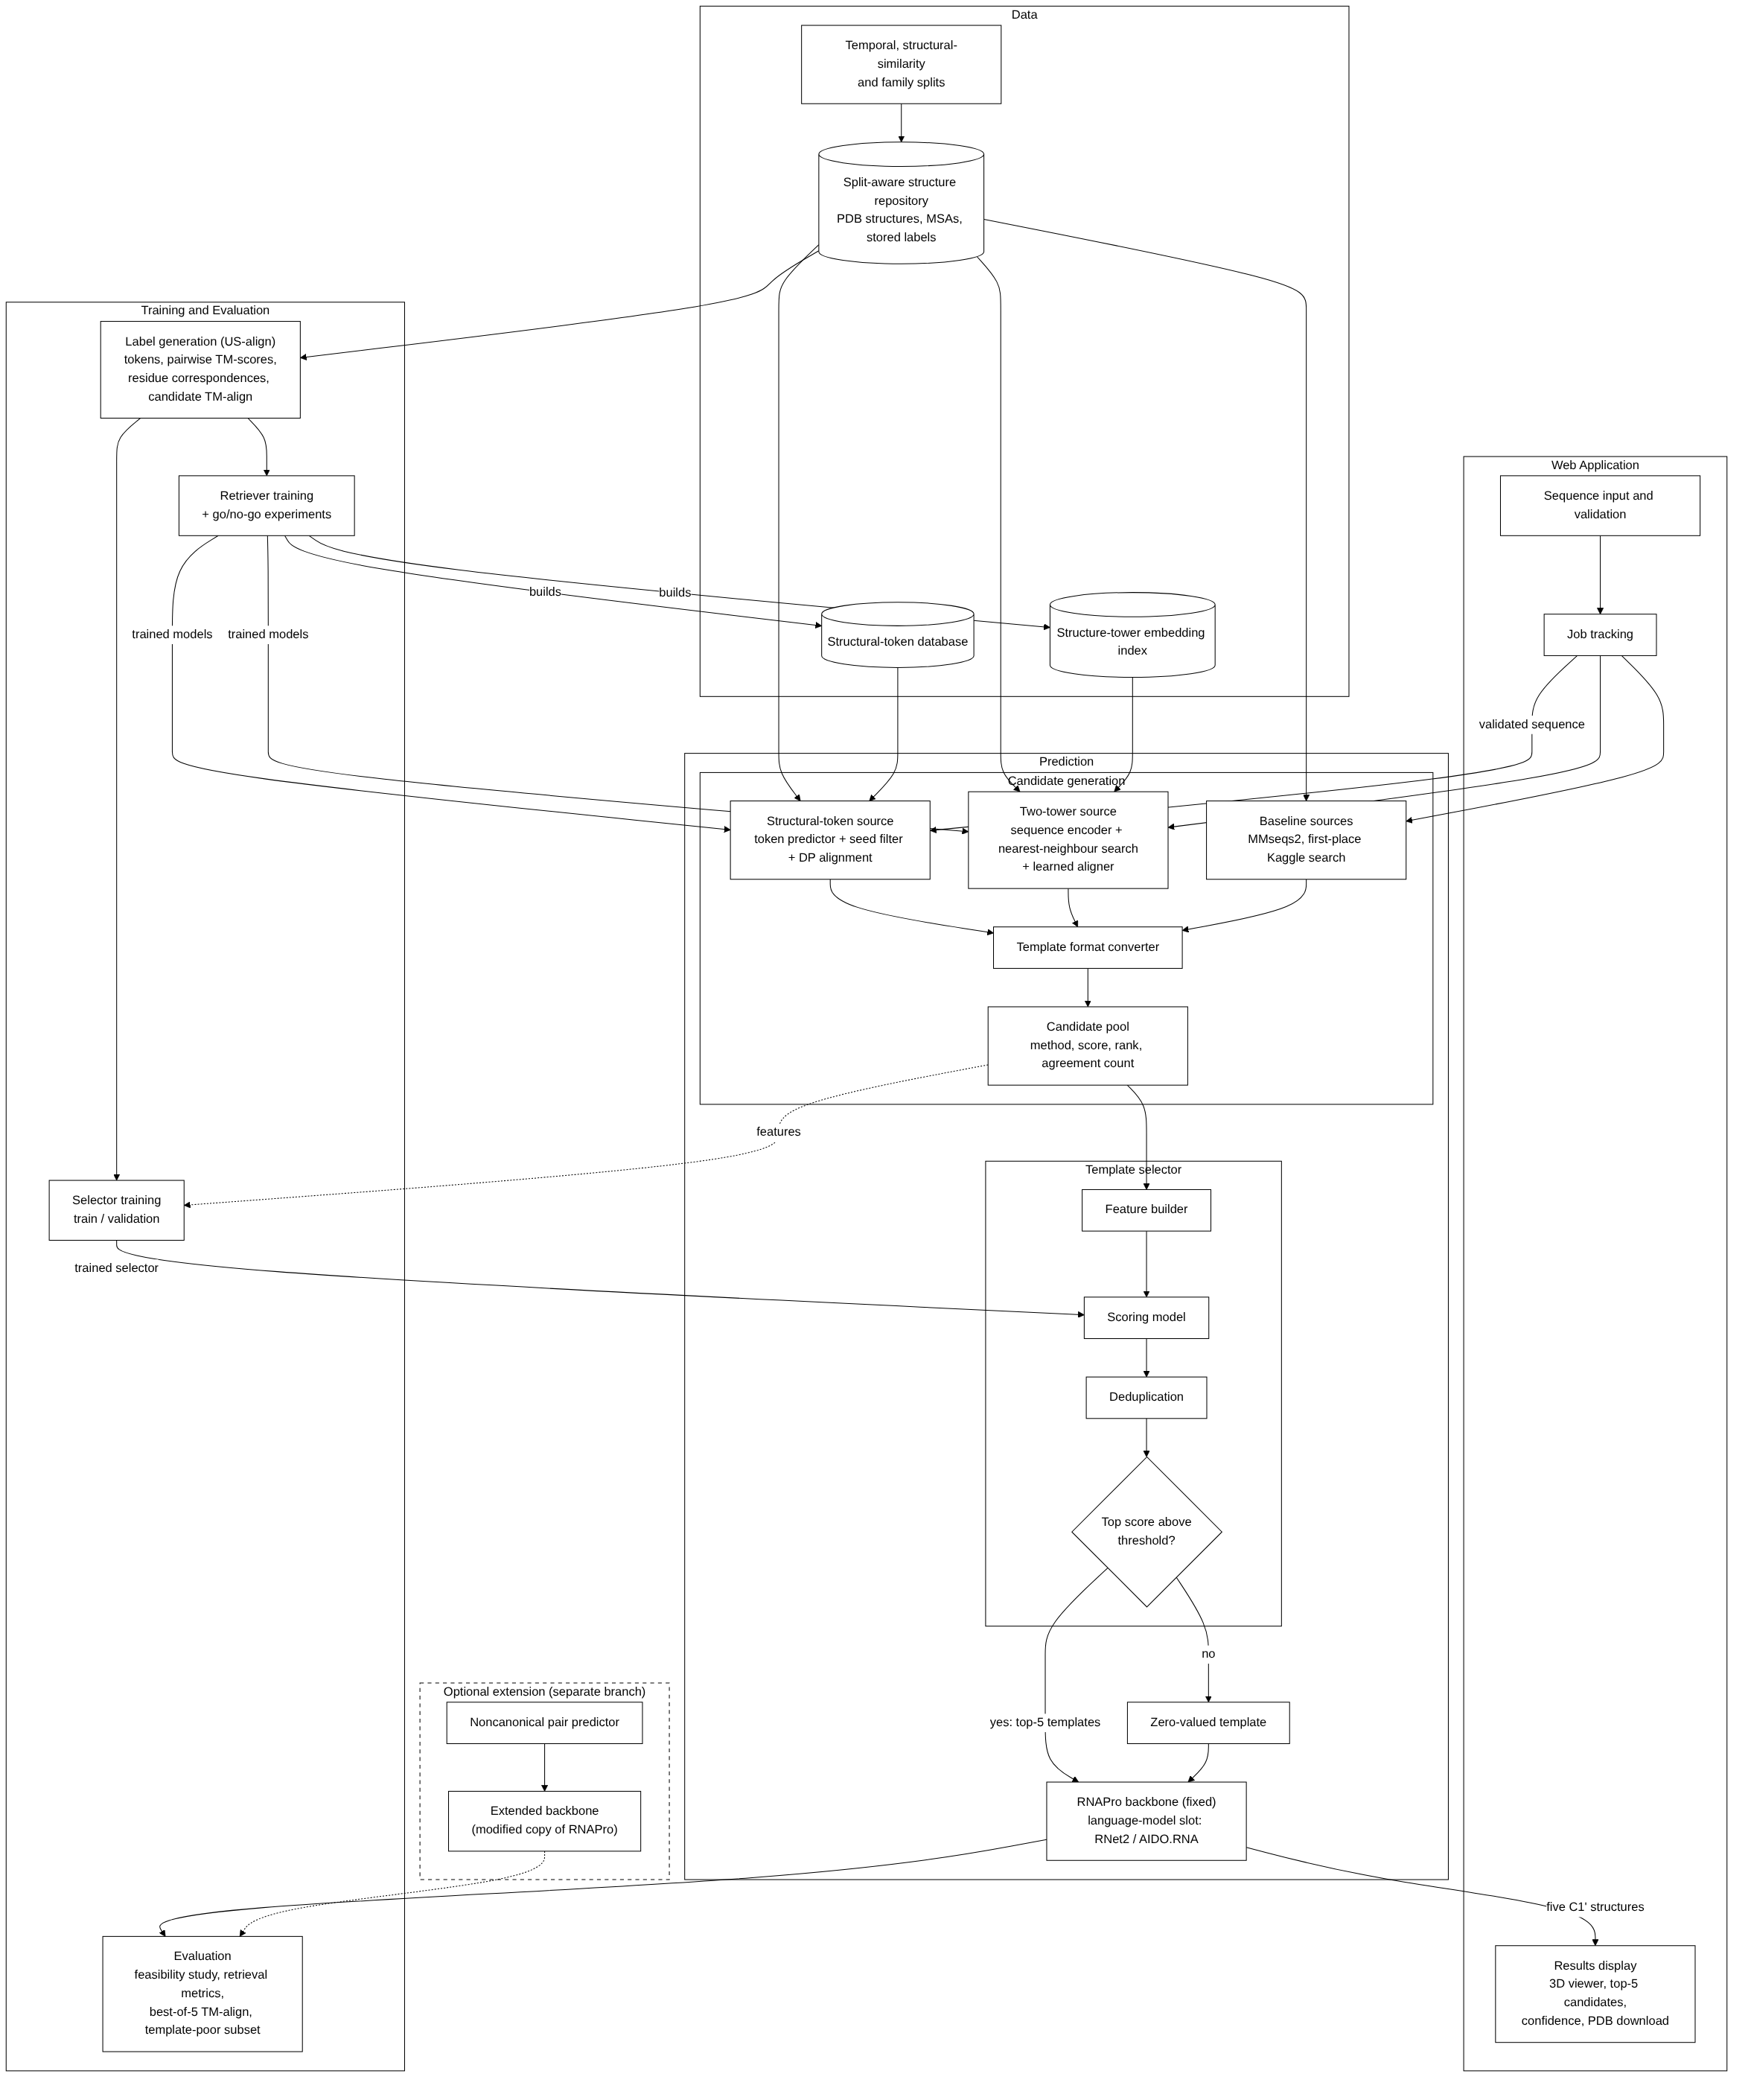
\includegraphics[width=\textwidth,height=0.9\textheight,keepaspectratio]{Figures/RNA_Candidate_Generation_BW.png}
\caption{System architecture showing the data layer, learned candidate generation, template selector, RNAPro prediction backbone, training and evaluation path, and the web application.}
\label{fig:architecture}
\end{figure}

\subsection{Subsystem Architecture}
The candidate generation subsystem deserves a closer look because it is made up of several independent parts. It consists of a set of template source modules, one per search method, and a pooling module. The sources are sequence similarity (covering MMseqs2 and Rfam with Infernal), family lookup, language-model embedding similarity, secondary-structure-aware similarity, motif or local search, and the first-place Kaggle search as a baseline source. Every source takes the same input, a target and the legal structure database, and returns candidates in the same format. Each candidate carries the identifier of the source structure, a residue mapping to the target, the method name, and that method's native score and rank. Sources do not call each other and share no state, so they can run independently and in parallel. The pooling module merges their outputs, notices when two methods have returned the same template, and records how many methods agreed. This agreement count is one of the selector's features.

The selection subsystem also has distinct parts. A scoring module applies the trained ranking or regression model to each candidate's feature vector. A deduplication module then computes TM-align between high-scoring candidates and drops any that are near copies of a better-scored one, so the five templates we keep are diverse and don't repeat the same fold. Finally, a thresholding module compares the top score with the value tuned on validation data and decides whether to use the zero-valued template instead. These three modules run in a fixed order and each one can be switched off for ablation, which lets us report the effect of deduplication and of the fallback separately.

\section{Architectural Strategies}
This section describes the strategies that shape the overall organization of the system, and the alternatives we considered for each.

\subsection{Fixed Backbone, Changes at Inference Only}
Our central strategy is to leave RNAPro's architecture, training recipe and training template pool unchanged and put all new work at inference. This supports controlled comparison, since the training distribution is identical across all conditions and a gain can be attributed to template choice. It also fits our compute constraint, because training the selector on precomputed features and labels is far cheaper than retraining a model this size. The main alternative was to enlarge the training pool with the new templates so the model could adapt to them. That might give higher accuracy, but it needs resources we don't have and it removes the clean attribution, so we didn't adopt it. The cost of our strategy is that the backbone may work better with the kind of templates it was trained on than with the ones our selector picks. We accept this and note it as a limitation.

\subsection{Common Interface for Interchangeable Components}
The second strategy is to put each template source and each language model behind a common interface. Every source implements the same operation, returning candidates in the shared format for a given target, and every language-model adapter exposes the same single and pair representations to the backbone. We expect the set of methods and models to change after pilot experiments, and adding a new one should not require touching the pipeline. We did consider writing each method directly into the pipeline. That would have been quicker at first, but it would make ablations error-prone and make it hard to evaluate a single method alone. The approach resembles the strategy pattern, where several algorithms with the same signature can be swapped at run time. For language models with no native pair-level outputs, the adapter is where pair features are derived, so that decision stays in one place and is reported as our own design choice.

\subsection{Split Enforcement at the Data Access Layer}
The third strategy is to enforce the temporal or structural-similarity split inside the structure repository instead of in the calling code. Every read takes a target and returns only structures that are legal for it, so no search, labeling step or training step can accidentally see a forbidden structure. The alternative was to filter results after retrieval. It is simpler to write, but it risks leakage whenever a new component forgets the filter. A single enforcement point is easier to verify and audit, and since the validity of the whole evaluation depends on it, we decided the small loss of flexibility was acceptable. Test targets go through the same layer and are released for scoring only once.

\subsection{Precomputed and Cached Labels and Features}
The fourth strategy deals with cost. TM-align labels for all candidates against all training and validation targets are expensive to compute, and candidate searches are slow. We compute both once, store them with the software versions and settings that produced them, and reuse them across all selector experiments. Recomputing on demand would make every experiment slow and make results harder to reproduce. The trade-off is storage, plus the need to invalidate stored results when a source or setting changes. We handle this by keying stored results on a record of the configuration that produced them.

\subsection{Error Detection and Recovery}
The last strategy is about failure handling. A search method may fail or return nothing for a given target, and the design treats this as a normal case. The pooling module accepts whatever the other sources return, and since the selector includes the finding method as a feature, a missing source makes the candidate list weaker but does not stop the run. If the pool is empty, or the top score falls below the threshold, the system uses the zero-valued template, which matches RNAPro's behavior when no suitable template exists. Failures are logged with the target and source identifiers so we can report them when analyzing results. We rejected the alternative of stopping on any failure, because a long evaluation run should not be lost to one unusual sequence.

\section{Domain Model/Class Diagram}
The domain model is built around a small number of classes that mirror the data flowing through the pipeline. A \texttt{Target} class represents an RNA to be predicted and holds its sequence, release-date cutoff and, when available, its experimental structure. A \texttt{Candidate} class represents a possible template. It holds the source structure identifier, the residue mapping to the target, the name of the method that found it, that method's native score and rank, and a feature vector once one has been built. A \texttt{SelectionResult} class holds an ordered list of at most five template identifiers, or a flag for the zero-valued template.

Candidate generation is modeled with an abstract \texttt{TemplateSource} class that declares a single search operation taking a \texttt{Target} and a \texttt{StructureRepository}. Concrete subclasses implement it for sequence similarity, family lookup, embedding similarity, secondary-structure-aware similarity, motif search and the Kaggle baseline. A \texttt{CandidatePool} class aggregates the outputs of the sources and computes the agreement count. The \texttt{StructureRepository} class owns access to structures and alignments, and all of its read operations take a \texttt{Target}, so the split rule is applied on every call. A \texttt{FeatureBuilder} class creates feature vectors from candidates, and a \texttt{LabelStore} class holds the stored TM-align values. The \texttt{Selector} class has a scoring model, a deduplication step and a threshold, and produces a \texttt{SelectionResult} from a \texttt{CandidatePool}.

{\sloppy On the prediction side, a \texttt{PredictionBackbone} class wraps RNAPro and accepts a \texttt{Target}, a \texttt{SelectionResult} and a \texttt{LanguageModelAdapter}. \texttt{LanguageModelAdapter} is an abstract class with concrete subclasses for RNet2, AIDO.RNA and any later models, each exposing single and pair representations. An \texttt{Evaluator} class compares predicted structures with experimental ones through US-align and aggregates results by condition and by subset, including the template-poor subset. As for relationships, \texttt{CandidatePool} aggregates \texttt{Candidate} objects, \texttt{Selector} uses \texttt{FeatureBuilder} and \texttt{LabelStore} during training, and \texttt{PredictionBackbone} depends on \texttt{LanguageModelAdapter}. \texttt{TemplateSource} and \texttt{StructureRepository} are linked by a dependency, since every source reads through the repository.\par}

Figure~\ref{fig:classdiagram} shows the domain model and the relationships between these classes.

\begin{figure}[!htbp]
\centering
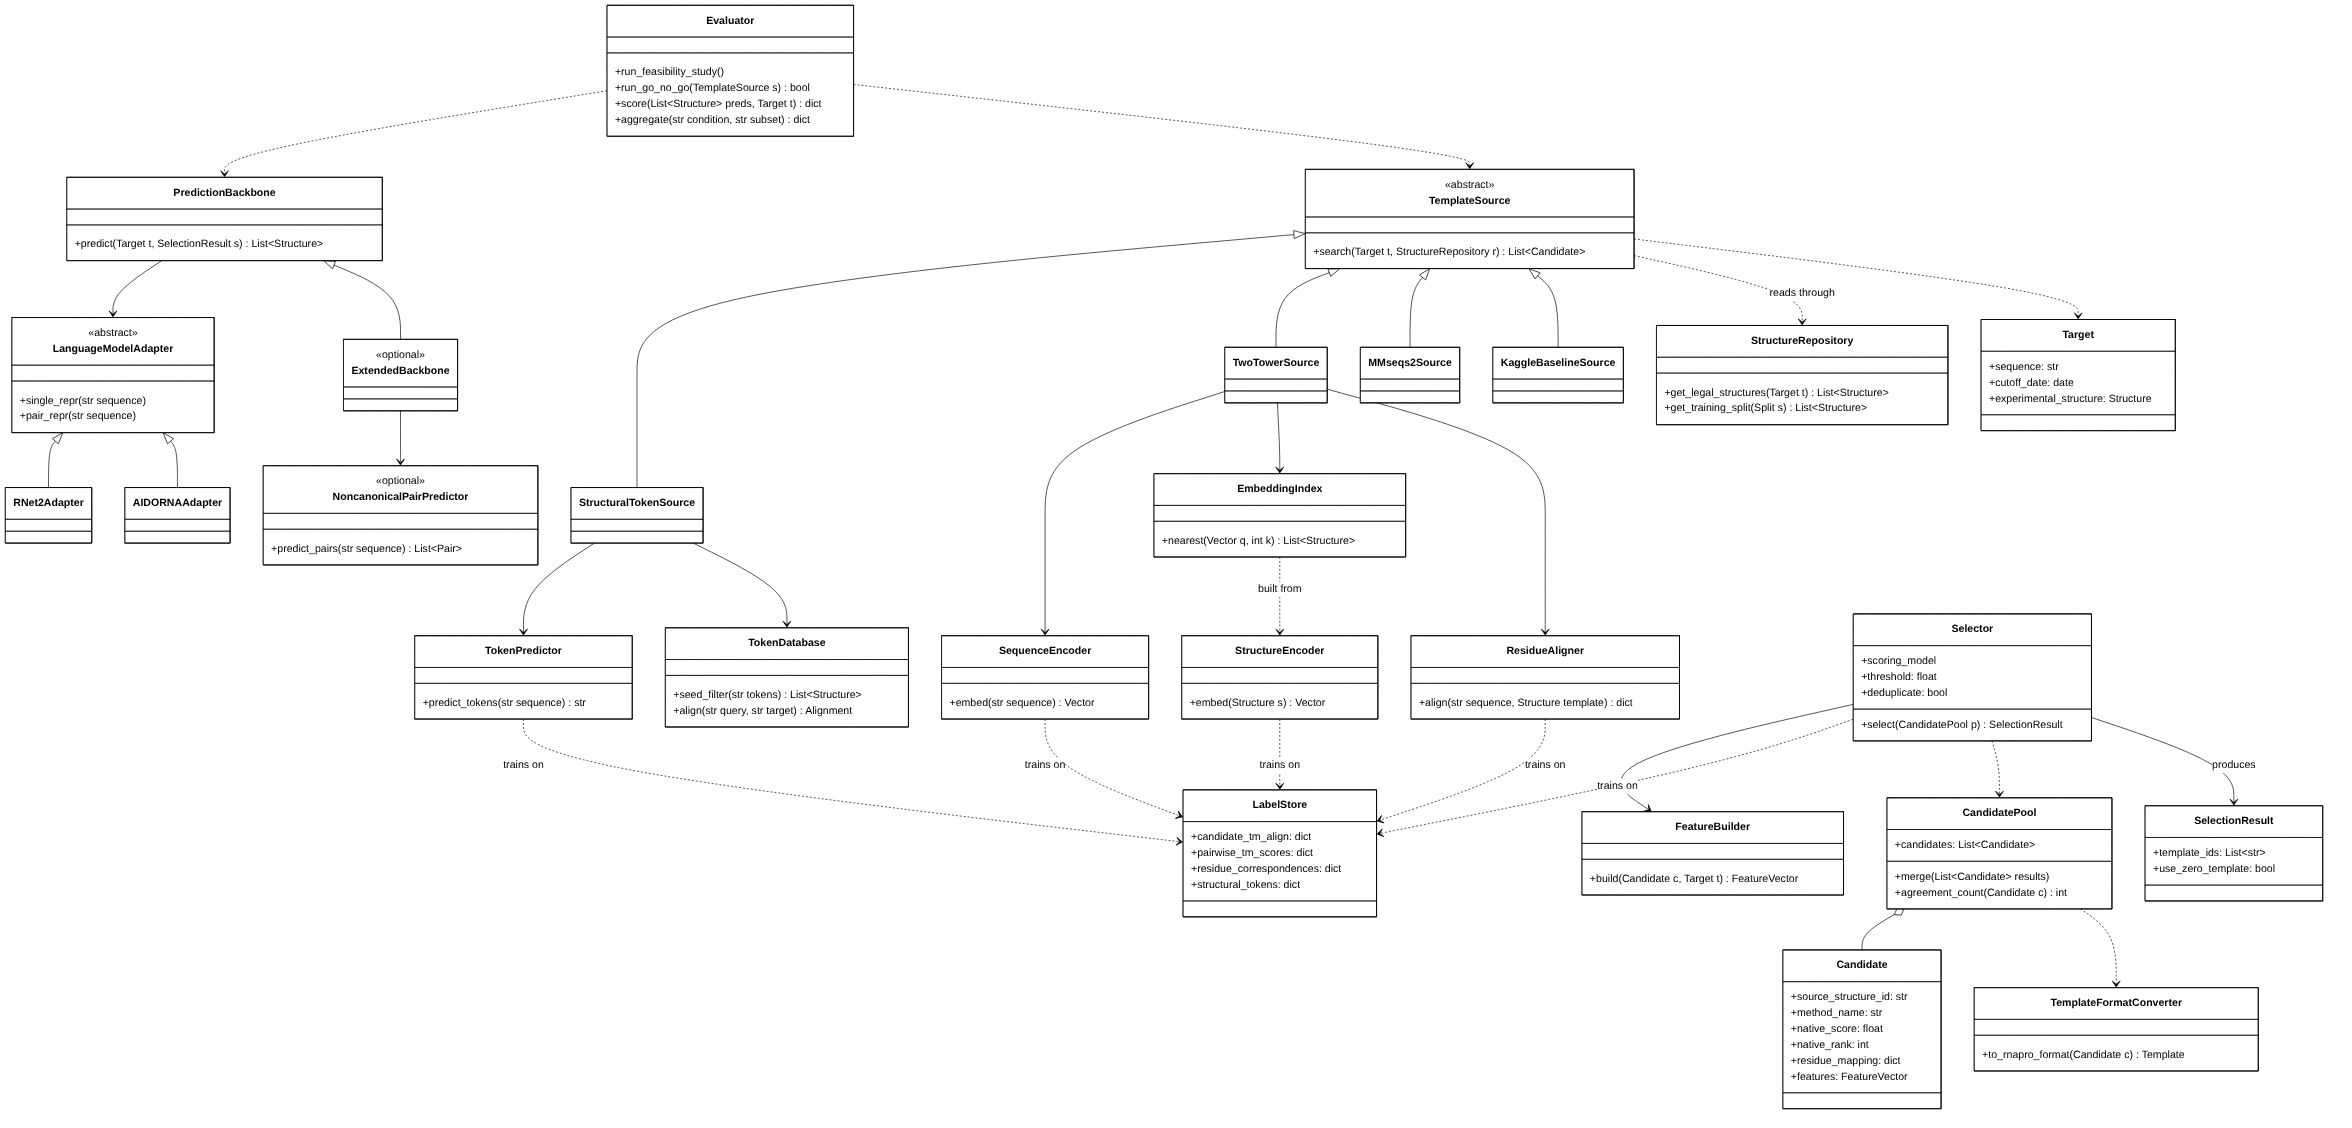
\includegraphics[width=\textwidth]{Figures/ClassDiagram.png}
\caption{Domain model and class diagram of the template-retrieval and selection system.}
\label{fig:classdiagram}
\end{figure}

\section{Policies and Tactics}
This section describes the design policies and tactics that affect the details of the implementation.

\subsection{Tools}
For tools, we plan to use Python, because the backbone and its public release are built on PyTorch, and to use established command-line tools for search and scoring, namely MMseqs2, Infernal with Rfam, and US-align. Staying with these keeps us close to the cited work, which makes our baseline reproduction more faithful. The selector will start with a simple model from a standard machine learning library, and we will only move to a more complex one if validation results justify it. Any change to these choices during development will be reported.

\subsection{Engineering Trade-offs}
When it comes to engineering trade-offs, we favor reproducibility over speed. Random seeds are fixed, software versions and tool settings are recorded with every stored result, and the training schedule is held constant across all compared conditions. Our coding conventions are modest: a consistent style checked automatically, short single-purpose functions, and descriptive names that match the terms used in this report so the code can be traced back to the design.

\subsection{Requirements Traceability and Testing}
For requirements traceability, each experimental condition in the evaluation protocol maps to a named configuration that selects a template source set, a selector mode and a language model. With this mapping, any reported number can be traced to the configuration that produced it. For testing, we plan unit tests for each template source on a few sequences with known answers, and a test that the structure repository does not return any structure released after a target's cutoff. We also plan a test that the selector falls back to the zero-valued template when the pool is empty, and a check that our reproduced baseline falls in a plausible range compared with the published figures before we trust any later results. The leakage test matters most, because the validity of the whole evaluation depends on it.

\subsection{Maintenance and Build}
For maintenance, adding a new template source or language model only requires implementing the shared interface and registering a configuration, with no change to the pipeline. The source code is organized into directories that match the components: template sources, the structure repository, features and labels, the selector, the backbone wrapper with the language-model adapters, and evaluation. Configurations and stored results are kept separately. The deliverables are built by running the stages in order. First the baseline is reproduced, then candidates and labels are generated and cached, and then the selector is trained and tuned on validation data. After that the language-model comparison is run, and the last stage scores the test split once.

\section{Conclusion}
This chapter described a design in which the RNAPro backbone stays fixed and the new work sits in components around it, such as candidate generation and the template selector. The architectural strategies keep the backbone unchanged, give interchangeable components a common interface, enforce the data split at the data access layer, cache labels and features, and handle failures by falling back to the zero-valued template. The class diagram models the data and the components, and the policies set the tool choices and favor reproducibility over speed.

\clearpage


\chapter{Implementation and Test Cases}
\label{ch:impl}
For each chapter, provide a paragraph of introduction and at the end, a paragraph of conclusions. (Not the programming code but the algorithmic and procedural details especially related to the hidden/ backend algorithms that are not covered in the design)
\section{Implementation}
\label{sec:impl}
This section describes the prototype we developed during FYP-1. The central contribution and novelty of the project is its template-finding layer, which consists of six template search methods implemented by us, two new learned retrieval methods (a two-tower retriever with a learned aligner, and a sequence-to-structural-token retriever), and a learned template selector that chooses among the candidates they return. Our implementation of RNAPro \cite{leerna} is the structure prediction model through which every template-finding condition is evaluated. We implemented and trained this model ourselves, so a change in template choice can be measured all the way to the final 3D structure and not only at the retrieval stage.

The prototype is organised as a pipeline of stages that share data through a common store. The data and split management stage loads structures, sequences and multiple sequence alignments (MSAs) and enforces the temporal and family-held-out splits. Label generation then computes, once, the structural labels used for training and evaluation. In the candidate generation stage, all template-finding methods run behind one interface and their outputs are pooled, after which the learned template selector reduces the pool to an ordered set of at most five templates or requests the zero-valued template. Our RNAPro model then produces five C1$'$ structures, the 3D validation engine based on gRNAde \cite{joshi2025grnade} ranks these candidates and assigns a confidence value, and the evaluation stage scores predictions against experimental structures. A language-model comparison module swaps the language model used inside our RNAPro model under controlled conditions, and the web application exposes the inference path to researchers.

Each subsection below first explains the algorithm or procedure we implemented and then gives a ``Platform and APIs'' paragraph naming the tools, versions, commands, file formats, storage and hardware used. The whole prototype is written in Python 3.11 with PyTorch 2.3 and CUDA 12.1, managed in a single conda environment under Git version control. Run settings are kept in YAML configuration files, and every cached result is keyed on a hash of the configuration and tool versions that produced it.

\subsection{Data and Split Management}
\label{sec:impl-data}
The data layer brings four sources into one consistent representation. RNA chains come from the Protein Data Bank (PDB) together with their initial release dates, and the Kaggle Stanford RNA 3D Folding data supplies target sequences and their experimental C1$'$ coordinates. MSAs are produced with rMSA, and we normalise every alignment by converting T to U and removing columns that are gaps in the query. The Eigen dataset is added for the second stage of our RNAPro training. Every chain is stored as a sequence, a per-residue array of C1$'$ coordinates with a mask for unresolved residues, a release date and, where available, the full-atom model needed later by secondary-structure annotation and validation. Modified nucleotides are mapped to their parent base, and chains that are shorter than a minimum length or have too few resolved C1$'$ atoms are discarded.

We remove redundancy by clustering chains on sequence identity, so that near-identical copies of the same molecule do not inflate the database or leak between splits. Two splits are then built on top of the cleaned and clustered data. In the temporal split, each target has a cutoff date, and only structures released before that date may be used as templates or for training. In the family-held-out (structural-similarity) split, built with RNA3DB, chains are grouped into components that share sequence or structural similarity, and whole components are assigned to the training, validation or test set. This means no family appears on both sides of the split, which makes it our test of template-poor RNAs.

The split is enforced in the data access layer and not in the calling code. The \texttt{StructureRepository} class answers every read with respect to a target, so a search method, a labelling job or a training loader can only receive structures that are legal for that target. The test split is locked behind a flag and is released for scoring once. The split-building procedure is as follows.

\begin{enumerate}
\item Parse every PDB and Kaggle structure, extract chain sequences, C1$'$ coordinates and release dates, and write them to the structure store.
\item Normalise sequences (T to U, modified residues to parent bases) and drop chains that fail the length and coverage filters.
\item Cluster the remaining chains by sequence identity and record a cluster identifier for each chain.
\item For the temporal split, attach a cutoff date to each target and define its legal set as all chains released before that date, excluding the target's own entry.
\item For the family-held-out split, run RNA3DB to obtain similarity components and assign each whole component to one of the training, validation or test sets.
\item Store split assignments in the database and expose them only through the \texttt{StructureRepository.legal\_structures(target)} read path.
\end{enumerate}

\textbf{Platform and APIs.} Structures are parsed from mmCIF files with gemmi 0.6.x (\texttt{gemmi.read\_structure}, then iteration over models, chains and residues to read the \texttt{C1'} atom), with Biopython 1.84 \texttt{Bio.PDB.MMCIFParser} kept as a fallback parser. Release dates are read from the \texttt{\_pdbx\_audit\_revision\_history} category of each mmCIF file. The PDB mirror is downloaded with \texttt{rsync} from the wwPDB archive, and the Kaggle data with the Kaggle command-line client (\texttt{kaggle competitions download -c stanford-rna-3d-folding}), which provides \texttt{train\_sequences.csv} and \texttt{train\_labels.csv} with C1$'$ coordinates. MSAs are stored as A3M/FASTA files. Clustering uses MMseqs2 \cite{steinegger2017} (\texttt{mmseqs easy-cluster} with \texttt{-{}-min-seq-id 0.8 -c 0.8 -{}-cov-mode 0}), and the family-held-out split uses the RNA3DB command-line tool (\texttt{rna3db parse}, \texttt{rna3db cluster}, \texttt{rna3db split}). Tabular data are handled with pandas 2.x and stored as Parquet files through pyarrow, while targets, structures and split assignments are mirrored in PostgreSQL 16 in the \texttt{TargetRNA}, \texttt{Structure}, \texttt{DataSplit} and \texttt{SplitAssignment} tables of our ERD. This stage runs on CPU nodes of the university cluster.

\subsection{Label Generation}
\label{sec:impl-labels}
Label generation produces the structural ground truth that the learned components are trained on and that the evaluation relies on. We compute three kinds of label. The first is a pairwise structural comparison between chains: US-align is run on the C1$'$ atom in its sequence-independent mode, which returns a TM-score normalised by the length of the reference chain, an RMSD over aligned residues and a residue-to-residue alignment. These pairwise TM-scores and alignments are the training targets of New Method 1 (Section~\ref{sec:impl-nm1}) and provide the substitution statistics used by New Method 2 (Section~\ref{sec:impl-nm2}). The second is a per-nucleotide structural token produced by the RiboSeek encoder \cite{wang2026riboseek}, which describes the local spatial neighbourhood of each nucleotide as one symbol from a fixed vocabulary, and these tokens are the training targets of New Method 2. The third is a quality label for every candidate structure. Each candidate template, after mapping onto the target, and each predicted structure is compared with the target's experimental structure by US-align, and the resulting TM-score and RMSD are the labels for the template selector and the scores used in evaluation.

All labels are expensive to compute and are needed many times, so we compute them once and cache them. Each cached entry is keyed on the identifiers of the two structures, the US-align or RiboSeek version and the exact settings used, so a label is recomputed only if one of these changes. Labels for test targets are generated only when the test split is released for scoring. The procedure for structural labels is as follows.

\begin{enumerate}
\item Write each chain involved in a comparison to a C1$'$-only PDB file, with the atom named \texttt{C1'} and residues numbered consecutively.
\item Look up the pair in the label cache; if a valid entry exists, return it.
\item Otherwise run US-align on the pair in sequence-independent mode on the C1$'$ atom and parse the TM-score (normalised by the reference length), the RMSD, the number of aligned residues and the residue alignment.
\item Convert the alignment into a list of index pairs between target and template residues and store it with the scores.
\item For structural tokens, pass each chain through the RiboSeek encoder and store one token per nucleotide, using a reserved symbol for residues with missing coordinates.
\end{enumerate}

\textbf{Platform and APIs.} US-align is compiled from its C++ source (release 20241201) and called as \texttt{USalign model.pdb native.pdb -mol RNA -atom " C1'" -outfmt 2} for tabular scores, with \texttt{-outfmt 1} used when the residue alignment is needed; sequence-independent superposition is the default behaviour, and \texttt{-TMscore 0} is set explicitly. The C1$'$-only PDB files are written with gemmi's structure writer. Calls are run in parallel through Python's \texttt{concurrent.futures.ProcessPoolExecutor} across 32 CPU cores. Structural tokens are produced with the RiboSeek Python API (\texttt{riboseek.encode(structure)} for single chains and \texttt{riboseek build-db} for whole databases) using the RS-20 and RS-80 vocabularies. Labels are stored in Parquet files and in the \texttt{TmalignLabel} table of our ERD, with the producing tool version and settings recorded alongside each row. This stage runs on CPU only.

\subsection{Template-Finding Methods}
\label{sec:impl-search}
Template finding is the core of the project. We implemented six independent search methods that each look for useful templates from a different angle: sequence, covariance-model homology, family membership, language-model embeddings, secondary structure and local motifs. All six sit behind one common interface, the abstract \texttt{TemplateSearchMethod} class, whose single operation \texttt{search(target, legal\_structures)} returns a list of candidates in a shared format. Every candidate records the identifier of the source structure and chain, the name of the method that found it, that method's native score (for example an E-value, a bit score or a cosine similarity), its rank within the method, and a residue mapping from target positions to template positions. Since every method produces the same format, methods can be run alone, in any combination or in parallel, and a new method can be added without changing the rest of the pipeline. In the evaluation, only MMseqs2 used alone and the first-place Kaggle template search, which we also implemented, act as comparison baselines.

Two safeguards are applied to every method. A method only receives the legal structures returned by the data access layer for the current target, and self-hits are removed: any candidate whose source entry is the target itself, or belongs to the same PDB entry or sequence cluster as a test target, is discarded before the candidate is returned. After all methods have run, the \texttt{CandidatePool} class merges their outputs, recognises when two or more methods returned the same template chain and records the number of methods that agree, which becomes one of the selector's features.

\textbf{Method 1: MMseqs2 sequence search.} The target sequence is searched against a nucleotide database of the legal chains with MMseqs2 \cite{steinegger2017}. Hits are ranked by E-value, and the residue mapping is read from the alignment start positions and the CIGAR string. As this is the fastest and most common approach, MMseqs2 used alone also serves as the simple baseline in the evaluation, and it supplies 40 of the 45 templates in the training pool of our RNAPro model.

\textbf{Method 2: Infernal and Rfam covariance-model homology search.} Covariance models capture both sequence conservation and base pairing, so they can detect distant homologues that sequence search misses. We first scan the target against all Rfam \cite{kalvari2018} covariance models with Infernal \cite{nawrocki2013} to identify its family or families. The legal chains are then searched with each matching covariance model, and the target and each hit are aligned to the same model. The residue mapping comes from matching residues that fall into the same match-state column of the model, and hits are ranked by bit score.

\textbf{Method 3: Family lookup through the Rfam-to-PDB mapping.} Rfam publishes a mapping from each family to the PDB chains that contain a member of that family. Given the family identified for the target in Method 2, this method lists all legal PDB chains annotated with the same family, even if they would not score highly in a direct search. Each listed chain is aligned to the family covariance model to obtain the residue mapping, and the native score is the chain's family bit score.

\textbf{Method 4: Language-model embedding similarity.} Following the embedding-based alignment (EBA) approach \cite{pantolini2024}, each nucleotide of the target and of every legal chain is represented by a contextual embedding from a pretrained RNA language model, RiNALMo \cite{ref:Penic:2024}. For a fast shortlist, we summarise each chain by its mean-pooled embedding and retrieve the nearest chains by cosine similarity. For each shortlisted chain, a residue-by-residue similarity matrix is built from the per-nucleotide embeddings, and a global alignment is computed on this matrix with dynamic programming. The alignment score is the native score, and the alignment gives the residue mapping.

\textbf{Method 5: Secondary-structure-aware search.} The secondary structure of the target is predicted in dot-bracket form with ViennaRNA RNAfold, and the secondary structures of legal chains are annotated from their full-atom 3D models. A single-sequence covariance model is built from the target sequence and its predicted structure with Infernal and searched against the legal chains, so that hits must agree with the target's base-pairing pattern as well as its sequence. Hits are then re-scored with BEAGLE, which aligns secondary structures directly, and the structural alignment provides the residue mapping.

\textbf{Method 6: Motif and local template search.} Many targets have no single good global template but contain local motifs that have been solved elsewhere. Following the Vfold precedent, the target's predicted secondary structure is decomposed into hairpin loops, internal loops and multi-way junctions. The legal structures are decomposed in the same way into a motif library indexed by motif type and loop lengths. Each target motif is matched against library motifs of the same type and size, and matches are ranked by sequence agreement in the loop and closing pairs. A returned candidate covers only the residues of its motif, and the rest of the target is masked as uncovered in the residue mapping.

\textbf{First-place Kaggle template search (comparison baseline).} We implemented the template search of the first-place solution of the Stanford RNA 3D Folding competition, following its public write-up and code, and restricted it to the legal structures of each target. It provides the remaining 5 templates in the 45-template training pool of our RNAPro model and is the main comparison baseline for our template-finding layer.

The search procedure for a single target is as follows.

\begin{enumerate}
\item Request the legal structure set for the target from the data access layer.
\item Run each enabled \texttt{TemplateSearchMethod} on the target and its legal set, in parallel.
\item Convert each method's raw output into the common candidate format with method name, native score, rank and residue mapping.
\item Remove self-hits and any candidate that fails the legality check.
\item Merge all candidates in the \texttt{CandidatePool}, collapse duplicates of the same template chain and record the number of agreeing methods.
\item Store the pooled candidates; if a method fails or returns nothing, log the failure and continue with the other methods.
\end{enumerate}

\textbf{Platform and APIs.} Method 1 uses MMseqs2 release 15-6f452: the legal chains are indexed with \texttt{mmseqs createdb} and searched with \texttt{mmseqs easy-search target.fasta legal\_db hits.m8 tmp -{}-search-type 3 -s 7.5 -e 10 -{}-max-seqs 1000 -{}-format-output "query,target,evalue,bits,qstart,qend,tstart,tend,cigar"}. Databases are built per cutoff-date bucket so that targets with the same cutoff share one index. Methods 2, 3 and 5 use Infernal 1.1.5 with Rfam 15.0: \texttt{Rfam.cm} is prepared with \texttt{cmpress}, the target is scanned with \texttt{cmscan -{}-rfam -{}-cut\_ga -{}-nohmmonly -{}-fmt 2 -{}-clanin Rfam.clanin -{}-tblout target.tbl Rfam.cm target.fasta}, legal chains are searched with \texttt{cmsearch -{}-tblout}, and alignments are produced with \texttt{cmalign -{}-outformat Stockholm}. Method 3 reads the Rfam family-to-PDB mapping file (\texttt{Rfam.pdb} / \texttt{pdb\_full\_region} table). Method 5 builds its single-sequence model with \texttt{cmbuild} from a Stockholm file carrying an \texttt{SS\_cons} line, predicts structures with the ViennaRNA 2.6 Python binding (\texttt{RNA.fold(seq)}), annotates 3D base pairs with DSSR or barnaba, and calls BEAGLE through its standalone release. Method 4 loads RiNALMo through its Python package and Hugging Face Transformers 4.4x with \texttt{output\_hidden\_states=True}, and indexes mean-pooled vectors with FAISS 1.8 (\texttt{IndexFlatIP} on L2-normalised vectors). Method 6 decomposes secondary structures with the forgi 2.0 bulge-graph API. Candidates are written to the \texttt{CandidateTemplate} table, and method metadata to the \texttt{SearchMethod} table, of our ERD. The sequence and covariance-model searches run on CPU nodes, and the embedding step of Method 4 runs on a Kaggle T4 GPU.

\subsection{New Method 1: Two-Tower Retrieval and Alignment}
\label{sec:impl-nm1}
New Method 1 is a learned retriever that predicts how structurally similar a database structure is to a target from the target's sequence alone. It adapts the TM-Vec and DeepBLAST approach \cite{hamamsy2024}, developed for proteins, to RNA, and all of its networks are trained from scratch on our own data. The method has two parts: a two-tower retrieval model that finds the candidate templates, and a learned alignment model that produces the residue mapping for each retrieved template.

The retrieval model has a sequence tower and a structure tower that map into the same vector space. The sequence tower is a Transformer encoder over nucleotide tokens with learned positional encodings, and its per-residue outputs are mean-pooled and projected to a fixed-length vector. The structure tower is a geometric vector perceptron (GVP) graph neural network \cite{jing2021gvp} that operates on a graph with one node per nucleotide placed at its C1$'$ atom, with each node connected to its $k$ nearest neighbours in space. Node features combine the nucleotide identity (scalar) with unit vectors to the previous and next C1$'$ atoms (vector), and edge features combine radial-basis encodings of the distance (scalar) with the unit direction vector (vector). GVP layers are equivariant to rotation, so the pooled output is invariant to the orientation of the input structure. We train the cosine similarity between the sequence vector of a target and the structure vector of a template to equal the US-align TM-score between the target's own structure and that template, using an L1 loss. At inference only the target's sequence is needed. The structure vectors of all legal database chains are precomputed, so retrieval reduces to a nearest-neighbour search.

The alignment model turns a retrieved pair into a residue mapping. Per-residue embeddings from the two towers are combined by a small network into a match-score matrix, together with position-specific gap-open and gap-extend scores. A differentiable Needleman--Wunsch algorithm, in which the maximum in the dynamic-programming recursion is replaced by a log-sum-exp, produces a soft alignment matrix that gives the probability of each target residue being aligned to each template residue. We train this matrix with a cross-entropy loss against the residue alignments produced by US-align (Section~\ref{sec:impl-labels}). At inference a hard alignment is decoded with the ordinary Needleman--Wunsch traceback on the learned scores. If the learned aligner does not pass its validation check (Section~\ref{sec:testmetrics}, Metric 3), the method falls back to plain Needleman--Wunsch on the cosine similarities of the per-residue embeddings with fixed gap penalties.

The training and retrieval procedure is as follows.

\begin{enumerate}
\item From the training split, sample pairs of chains and look up their cached US-align TM-scores and residue alignments, balancing pairs across TM-score bins so that dissimilar pairs do not dominate.
\item Train the two towers jointly: encode one chain's sequence and the other chain's structure, compute the cosine similarity of the two vectors and minimise the L1 distance to the TM-score.
\item Freeze the towers and train the alignment model with the differentiable Needleman--Wunsch layer and a cross-entropy loss against US-align alignments.
\item Select the checkpoint with the lowest validation loss and check the go/no-go criteria for both the retriever and the aligner.
\item Encode every legal database chain with the structure tower and store the vectors in a nearest-neighbour index.
\item At inference, encode the target sequence, retrieve the top-$K$ chains by cosine similarity, filter them through the legality check, align each with the learned aligner (or the fallback) and return them in the common candidate format, with the predicted TM-score as the native score.
\end{enumerate}

\textbf{Platform and APIs.} Both towers are implemented in PyTorch 2.3. The structure tower uses PyTorch Geometric 2.5 for graph batching, \texttt{torch\_cluster.knn\_graph} with $k = 16$ to build edges, and the GVP layers from the \texttt{gvp-pytorch} reference implementation. The sequence tower uses \texttt{torch.nn.TransformerEncoder} with 6 layers, 8 heads and a model width of 256. The differentiable Needleman--Wunsch layer is written in PyTorch with \texttt{torch.logsumexp} over anti-diagonals so that it runs on the GPU and supports automatic differentiation. Training uses the AdamW optimiser with a learning rate of 1e-4, bf16 or fp16 mixed precision through \texttt{torch.autocast}, and a crop length of 512 nucleotides, on Kaggle T4 or P100 GPUs. Database vectors are stored as NumPy \texttt{.npy} files and indexed with FAISS \texttt{IndexFlatIP} on L2-normalised vectors. Model checkpoints are saved as \texttt{.pt} files with the optimiser state and step count.

\subsection{New Method 2: Sequence-to-Structural-Token Retrieval}
\label{sec:impl-nm2}
New Method 2 searches for templates in a structural alphabet and not in nucleotide space. RiboSeek \cite{wang2026riboseek} describes each nucleotide of a known structure with a discrete token that summarises its spatial neighbourhood, so two structures with similar folds produce similar token strings even when their sequences differ. A target has no known structure, so we trained a model that predicts the token string directly from the sequence, and then use it to search the token strings of the legal database. This mirrors ProstT5 \cite{heinzinger2024prostt5}, which translates protein sequences into a structural alphabet for search, and is to our knowledge new for RNA templates.

The token predictor is a small sequence-labelling network trained from scratch. We implemented two architectures behind the same interface, a Transformer encoder and a 1D residual convolutional network (1D ResNet), and the better one on validation data is kept. The input is the one-hot or embedded nucleotide sequence, and the output is a probability distribution over the RiboSeek vocabulary at each position, so the model predicts one token per nucleotide. Structural tokens are strongly imbalanced, because tokens for regular helices are far more common than those for loops and junctions. To handle this, the model is trained with class-weighted cross-entropy in which each class weight is inversely related to its frequency in the training split. Before the predictor is used for retrieval it must pass a go/no-go check on held-out families: its per-nucleotide accuracy and macro-F1 must exceed two simple baselines, a majority-class predictor that always outputs the most common token and a nucleotide-identity predictor that outputs the most common token for each nucleotide type (A, C, G or U). If the predictor does not beat both baselines, the method is not used for retrieval and this is reported.

Search has two stages. In the shortlist stage, the token strings of all legal chains are indexed by spaced seeds, which are patterns of fixed length in which only some positions must match. Spaced seeds tolerate isolated token mismatches better than contiguous k-mers. Chains that share enough seed hits with the predicted target string are shortlisted. In the alignment stage, each shortlisted chain is aligned to the target token string with the Smith--Waterman local alignment algorithm, using a token substitution matrix and affine gap penalties. The substitution matrix is estimated as log-odds scores from how often two tokens are aligned in the US-align residue alignments of structurally similar training pairs. The Smith--Waterman score is the native score, and the token alignment directly gives the residue mapping between target and template.

The procedure is as follows.

\begin{enumerate}
\item Encode every chain in the training, validation and legal database sets into RiboSeek token strings (Section~\ref{sec:impl-labels}).
\item Train the token predictor on training-split sequences with class-weighted cross-entropy and select the checkpoint with the best validation macro-F1.
\item Evaluate accuracy and macro-F1 on held-out families against the majority-class and nucleotide-identity baselines, and stop if the go/no-go criterion is not met.
\item Build the spaced-seed index over the token strings of the legal database chains.
\item For a target, predict its token string, collect chains with at least the minimum number of seed hits and align each with Smith--Waterman.
\item Rank the aligned chains by score, convert the alignments to residue mappings and return them in the common candidate format.
\end{enumerate}

\textbf{Platform and APIs.} Token strings are produced with the RiboSeek Python API (\texttt{riboseek.encode} and \texttt{riboseek build-db}, with \texttt{riboseek search} used as a reference search on true tokens) using the RS-20 vocabulary. The predictor is implemented in PyTorch 2.3; the Transformer variant uses 4 encoder layers with a width of 256, and the ResNet variant uses dilated 1D convolutions with 8 residual blocks. Class weights are computed with \texttt{sklearn.utils.class\_weight.compute\_class\_weight} and passed to \texttt{torch.nn.CrossEntropyLoss(weight=...)}, and accuracy and macro-F1 are computed with \texttt{sklearn.metrics.accuracy\_score} and \texttt{f1\_score(average="macro")}. The spaced-seed index is a Python dictionary from seed keys to chain positions with the seed pattern \texttt{1101011}, and Smith--Waterman alignment uses the parasail 1.3 library with a custom matrix created by \texttt{parasail.matrix\_create} and the traceback function \texttt{parasail.sw\_trace\_striped\_16}. Training runs on Kaggle T4 or P100 GPUs, and token strings and the index are stored as Parquet and pickle files.

\subsection{Learned Template Selector}
\label{sec:impl-selector}
The pooled candidate list for a target can contain hundreds of templates from eight sources (the six search methods and the two new methods), each scored on a different scale. The learned template selector turns this list into the ordered set of templates that our RNAPro model receives. It predicts, for every candidate, how close that template is to the target's true structure, and keeps the best diverse ones.

The \texttt{FeatureBuilder} class describes each candidate with a fixed feature vector. The features are the finding method (one-hot), the method's native score and rank, the number of methods that returned the same template, the sequence identity between target and template over the mapped residues, the secondary-structure similarity between the target's predicted structure and the template's annotated structure (base-pair F1 over mapped positions), the target coverage (the fraction of target residues that the mapping covers), the language-model embedding similarity of the two sequences, and the TM-score predicted by New Method 1 (Section~\ref{sec:impl-nm1}). Native scores are converted to comparable forms (for example the negative logarithm of E-values) and all continuous features are standardised on the training split. The training label for each candidate is its cached US-align TM-score against the target's experimental structure (Section~\ref{sec:impl-labels}).

We introduced models in order of complexity. A linear regression on the TM-score and a logistic regression on whether the TM-score passes the correct-fold threshold of 0.45 are fitted first. Gradient-boosted trees are trained only if they improve the validation ranking measures enough to justify the added complexity, and the decision is recorded in the selector configuration. Cross-validation folds are grouped by target family so that candidates for the same family do not appear in both the training and validation folds. For comparison with the learned selector we implemented a heuristic picker, which takes the top hit from each method in a fixed priority order.

Selection for a target follows these steps.

\begin{enumerate}
\item Build the feature vector of every pooled candidate.
\item Score each candidate with the trained model and sort the candidates by predicted score in descending order.
\item Walk down the sorted list and discard any candidate that is a near-duplicate of one already kept, where two templates are near-duplicates if their mutual US-align TM-score exceeds a threshold or they come from the same sequence cluster.
\item Stop once five templates have been kept or the list is exhausted, and keep them in order, so that prediction $k$ of our RNAPro model uses the top-$k$ templates.
\item Compare the predicted score of the best template with a threshold tuned on the validation split; if no candidate passes it, or the pool is empty, return a flag requesting the zero-valued template instead.
\item Store the ordered template identifiers (or the zero-template flag) as the selection result for the target.
\end{enumerate}

\textbf{Platform and APIs.} The linear and logistic models use scikit-learn 1.5 (\texttt{LinearRegression}, \texttt{Ridge} and \texttt{LogisticRegression} inside a \texttt{Pipeline} with \texttt{StandardScaler}), and grouped cross-validation uses \texttt{GroupKFold}. Gradient-boosted trees use LightGBM 4.x, either \texttt{LGBMRegressor} on the TM-score or \texttt{LGBMRanker} with the \texttt{lambdarank} objective and target identifiers as query groups. Ranking quality on validation is measured with \texttt{sklearn.metrics.ndcg\_score} and Recall@$k$. Fitted models are saved with \texttt{joblib.dump}. The model path, feature list, threshold and near-duplicate setting are stored in the \texttt{SelectorConfig} table, the features in the \texttt{FeatureVector} table and the outputs in the \texttt{SelectionResult} and \texttt{SelectedTemplate} tables of our ERD. The selector trains and runs on CPU.

\subsection{Implementation of the RNAPro Model}
\label{sec:impl-rnapro}
Our RNAPro model is the structure prediction model that turns a target sequence, its MSA, language-model features and the templates chosen by our template-finding layer into 3D structures. We implemented the full RNAPro architecture \cite{leerna} ourselves, built its data pipeline and template encoder, and trained it with a two-stage schedule. The evaluation measures template-finding quality through the final predicted structure, so a faithful and well-trained implementation of this model is essential to the project, and it is one of its largest engineering components.

The model receives four inputs. The sequence is embedded as nucleotide tokens. The MSA from rMSA is embedded and processed by an MSA module that updates the pair representation. Language-model features come from RNet2, which is kept frozen: its single (per-nucleotide) and pair representations are taken from several layers, combined by layer-weighted averaging with learned softmax weights, projected to the widths of our trunk and injected into the single and pair streams through sigmoid gates, so that the model learns how much language-model information to admit at each position. The fourth input is the set of templates, handled by our template encoder. For each template, the residue mapping is used to place the template's C1$'$ coordinates onto target positions, a distogram is computed from the pairwise C1$'$ distances and discretised into distance bins, and the one-hot bins are combined with the template's nucleotide identities and projected into pair features. Positions that the template does not cover are masked, so the model does not treat missing residues as real distances. When no template is available, a zero-valued template with an all-zero mask is supplied, which is the same behaviour the selector requests through its fallback flag.

The trunk is a 48-block Pairformer. Each block applies triangle multiplicative updates (outgoing and incoming), triangle self-attention (around the starting and ending node), a pair transition, and single-representation attention with pair bias followed by a single transition. The trunk output conditions a diffusion module that generates C1$'$ coordinates. Starting from Gaussian noise, a denoising network conditioned on the single and pair representations iteratively removes noise over a fixed sampling schedule, producing one C1$'$ coordinate per nucleotide.

Training starts from the Protenix base checkpoints, which provide the initial weights of the Pairformer and diffusion module, while the template encoder and the language-model gates are newly initialised. Training has two stages. Stage 1 runs for 50,000 steps on the Kaggle data with a learning rate of 5e-4. Stage 2 adds the Eigen data and runs for a further 50,000 steps at a learning rate of 1e-4. The diffusion batch size is 8 and inputs are cropped to 512 nucleotides. For each training example, 4 templates are sampled from a fixed pool of 45 per target, made up of 40 from MMseqs2 and 5 from the first-place Kaggle search, so the model learns to use templates of varying quality. The loss combines a weighted mean-squared error on denoised C1$'$ coordinates, a smooth LDDT loss and a distogram loss on the pair representation. At inference the model is run five times, and prediction $k$ receives the top-$k$ templates from our selector, giving five candidate structures per target.

The original study trained RNAPro on eight GB300 GPUs, which is well beyond our compute, so we adapted training to fit our hardware without changing the model. Computation runs in bf16 mixed precision, which roughly halves activation memory. Activation checkpointing is applied to every Pairformer block, so activations are recomputed in the backward pass instead of stored. Gradient accumulation over several micro-batches reaches the target diffusion batch size of 8 on fewer GPUs. Training is distributed with data parallelism across the available GPUs, and checkpoints are written at fixed intervals with the model weights, optimiser state, learning-rate scheduler state, step count and random-number-generator states, so that an interrupted job resumes from exactly where it stopped. To confirm that our implementation is correct, we reproduce the published RNAPro baseline under the paper's settings and compare it with the reported mean TM-score of 0.640 (in the paper's text) and 0.648 (in its Table 2). All later comparisons use our own reproduced baseline.

The training procedure is as follows.

\begin{enumerate}
\item Load the Protenix base checkpoint into the Pairformer and diffusion module, and initialise the template encoder and language-model gates.
\item Precompute and cache the frozen RNet2 single and pair representations, the rMSA alignments and the 45-template pool for every training target.
\item For each training step, crop the target to 512 nucleotides, sample 4 templates from its pool, build the template features with coverage masks and assemble the input batch.
\item Run the forward pass in bf16 with activation checkpointing, compute the loss and accumulate gradients until the effective batch size is reached, then update the weights.
\item Save a full checkpoint at fixed intervals and evaluate on the validation split.
\item After 50,000 Stage 1 steps, add the Eigen data, lower the learning rate and continue for 50,000 Stage 2 steps from the last checkpoint.
\end{enumerate}

\textbf{Platform and APIs.} Our implementation builds on the Protenix codebase v0.5 and its released base checkpoint, in PyTorch 2.3 with CUDA 12.1. Mixed precision uses \texttt{torch.autocast(device\_type="cuda", dtype=torch.bfloat16)}, activation checkpointing uses \texttt{torch.utils.checkpoint.checkpoint} around each Pairformer block, and distributed training uses \texttt{torch.nn.parallel.DistributedDataParallel} launched with \texttt{torchrun -{}-nproc\_per\_node 4}. Gradient accumulation uses 2 micro-batches per optimiser step, and the optimiser is Adam with a warm-up followed by step decay. Checkpoints are saved every 1,000 steps as \texttt{.pt} files with \texttt{torch.save}, together with an exponential moving average of the weights. The RNet2 weights are loaded from their public Kaggle release, and their representations are cached in HDF5 files through h5py. Training metrics are logged to Weights \& Biases. Training runs on 4 $\times$ NVIDIA A100 80 GB GPUs on the university cluster or a cloud provider, and inference also runs on a single A100. Predicted C1$'$ coordinates are written as PDB files with gemmi and as CSV files in the Kaggle submission format, and are recorded in the \texttt{Prediction} table of our ERD.

\subsection{3D Validation Engine (gRNAde)}
\label{sec:impl-grnade}
The 3D validation engine ranks the candidate structures produced for a target and attaches a confidence value to the best one. It uses gRNAde \cite{joshi2025grnade}, a GVP-based inverse-folding model that, given an RNA backbone, outputs a probability for each nucleotide at each position. The idea is that a structure close to the true fold should make the target's own sequence likely. If gRNAde, shown a candidate structure, assigns a high likelihood to the sequence that was actually used to predict it, the candidate is consistent with that sequence. The engine can therefore score structures without needing the experimental structure, which is what the web application requires for new sequences.

The candidate set for each target contains the five structures from our RNAPro model and, where it is feasible to run, the structures predicted by DRfold2 \cite{ref:Li:2026}. For each candidate, the engine computes three quantities. The log-likelihood of the target's native sequence is computed by teacher forcing through gRNAde's autoregressive decoder, summing the log-probability of the correct nucleotide at each position. The perplexity is the exponential of the negative mean log-likelihood per nucleotide, so lower perplexity means a better fit. The sequence recovery is the average fraction of positions at which sequences sampled from gRNAde match the native sequence. Raw perplexity also depends on sequence length and composition, so we normalise scores within each target by converting them to z-scores across that target's candidates, and the normalised perplexity is the primary ranking score. Candidates are ranked by this score, near-duplicates (pairs whose mutual US-align TM-score is above a threshold) are removed, and the top five are kept. The score of the top candidate is mapped to a low, medium or high confidence level using thresholds tuned on the validation split, and this is the confidence value shown in the web application.

There is a representation gap between the two models. gRNAde builds its graph from three backbone atoms per nucleotide (P, C4$'$ and N1 for pyrimidines or N9 for purines), while our RNAPro model outputs only the C1$'$ atom. We bridge this gap with full-backbone reconstruction from the C1$'$ trace before scoring. For each nucleotide, a local reference frame is defined from the C1$'$ positions of the nucleotide and its two neighbours, and the P, C4$'$ and N1/N9 atoms are placed in that frame using average internal coordinates for that nucleotide type, estimated from high-resolution structures in the training split. The reconstructed backbone is then refined into a full-atom model with Arena to remove clashes and restore realistic geometry. The same reconstruction is applied to every candidate, including DRfold2 structures reduced to their C1$'$ trace, so that all candidates are scored on equal terms. As a check on the bridge, experimental structures are reduced to C1$'$, reconstructed and rescored, and their scores are compared with those of the original full-atom structures. As a secondary option, kept for comparison, we also implemented a variant of gRNAde's featuriser that builds the graph from C1$'$ atoms only and retrained its encoder on C1$'$-only inputs from the training split.

The scoring procedure for one target is as follows.

\begin{enumerate}
\item Collect the five structures from our RNAPro model and, if available, the DRfold2 structures.
\item Reconstruct P, C4$'$ and N1/N9 for every candidate from its C1$'$ trace and refine the result into a full-atom model.
\item Convert each reconstructed structure into a gRNAde input graph.
\item Compute the native-sequence log-likelihood by teacher forcing, the perplexity, and the sequence recovery over a fixed number of sampled sequences.
\item Normalise the perplexities within the target, rank the candidates and remove near-duplicates.
\item Keep the top five candidates, map the best score to a confidence level and store the scores.
\end{enumerate}

\textbf{Platform and APIs.} The engine uses the gRNAde codebase (the \texttt{geometric-rna-design} repository) with its released single-state checkpoint, running on PyTorch 2.3, PyTorch Geometric 2.5 and \texttt{torch\_cluster}. Structures are converted with the codebase's featuriser, the log-likelihood is computed from the decoder logits with \texttt{torch.nn.functional.log\_softmax}, and sequence recovery uses the model's sampling function with 16 samples per candidate at temperature 0.1. Backbone reconstruction is our own NumPy routine for atom placement, followed by Arena (\texttt{Arena input.pdb output.pdb 5}) for full-atom refinement. DRfold2 is run from its public repository on its default settings. Near-duplicates are detected with US-align as in Section~\ref{sec:impl-labels}. Scores are stored in the \texttt{Prediction} and \texttt{EvaluationScore} tables of our ERD, and the engine runs on a Kaggle T4 GPU or a single A100.

\subsection{Language-Model Comparison}
\label{sec:impl-lm}
The language-model comparison asks which RNA language model gives our RNAPro model the most useful features, under conditions controlled tightly enough that any difference can be attributed to the language model alone. The language model occupies a single slot in our RNAPro model, exposed through the abstract \texttt{LanguageModelAdapter} class. Every adapter takes a sequence and returns a single representation (one vector per nucleotide) and a pair representation (one vector per pair of nucleotides) from each of the model's layers, which the layer-weighted averaging and sigmoid gates of Section~\ref{sec:impl-rnapro} then consume. RNet2 is the default adapter. We implemented additional adapters for AIDO.RNA \cite{zou2024} and RiNALMo \cite{ref:Penic:2024}, and a no-language-model adapter that returns zeros with the gates closed, which serves as the ablation.

Some language models, such as AIDO.RNA and RiNALMo, produce only per-nucleotide outputs and have no native pair representation. For these, the adapter derives pair features from the single representation. Each per-nucleotide vector is first projected to a smaller width, the outer product of the projected vectors of nucleotides $i$ and $j$ is formed, and a linear projection maps it to the pair width expected by our RNAPro model. This derivation is our own design choice, so it is kept in the adapter and applied identically to every model without a native pair output.

To keep the comparison controlled, everything except the language model and its interface is held fixed. Each language model is frozen. Only the layer weights, the projections and the sigmoid gates that inject its features are retrained, while the Pairformer, diffusion module and template encoder of our trained RNAPro model are frozen. The training data, the template pool, the random seeds, the number of steps and the learning-rate schedule are the same for every model.

The procedure for each language model is as follows.

\begin{enumerate}
\item Implement an adapter that loads the model and returns its single representations, and its pair representations if it has them, from every layer.
\item If the model has no pair output, add the outer-product and linear-projection head that derives pair features.
\item Run the frozen model once over all training, validation and test sequences and cache its representations.
\item Load our trained RNAPro checkpoint, replace the language-model slot with the new adapter and reinitialise only the layer weights, projections and gates.
\item Retrain these parameters with the fixed data, templates, seeds and schedule, keeping all other weights frozen.
\item Evaluate on the validation split with the same metrics as Section~\ref{sec:impl-eval}, and evaluate the model chosen on validation once on the test split.
\end{enumerate}

\textbf{Platform and APIs.} RiNALMo and AIDO.RNA are loaded through Hugging Face Transformers 4.4x (\texttt{AutoModel.from\_pretrained(..., trust\_remote\_code=True)} with \texttt{output\_hidden\_states=True}), with AIDO.RNA also available through GenBio's ModelGenerator package and its \texttt{genbio-ai/AIDO.RNA-1.6B} checkpoint, and RiNALMo through its own Python package and the \texttt{giga-v1} weights. RNet2 is loaded from its public release as in Section~\ref{sec:impl-rnapro}. Cached representations are stored in fp16 in HDF5 files through h5py, one file per model and split. The gate retraining uses the same PyTorch 2.3 training code as our RNAPro model with a shorter schedule of 10,000 steps, fixed seeds set through \texttt{torch.manual\_seed}, \texttt{numpy.random.seed} and \texttt{random.seed}, and deterministic data ordering. Embedding extraction for the large models runs on a single A100 80 GB GPU, and each model's configuration is recorded in the \texttt{LanguageModel} table of our ERD.

\subsection{Evaluation}
\label{sec:impl-eval}
The evaluation module measures how much each template-finding condition improves the final structures predicted by our RNAPro model, and how good the retrieval is before prediction. The primary metric follows the Kaggle competition and the RNAPro paper. Each of the five predictions for a target is compared with the experimental structure by US-align on the C1$'$ atom, the best TM-score of the five is taken, and this best-of-5 TM-score is averaged over all targets. A TM-score above 0.45 is treated as a correct global fold. The module also reports the TM-score of each individual prediction, the C1$'$ RMSD of the best prediction, and per-target Z-scores, computed by standardising each condition's TM-score against the mean and standard deviation of all conditions on that target, so that hard and easy targets contribute equally to comparisons.

Retrieval is measured separately with Recall@$k$, the fraction of targets for which at least one of the top-$k$ candidates returned by a method (or chosen by the selector) has a US-align TM-score of at least 0.45 against the target's experimental structure, for $k$ equal to 1, 5 and 10. We compare results with a best-template upper bound, the TM-score of the single best legal template for each target according to US-align, which shows how close each condition comes to the best that template-based prediction could achieve. Targets whose best legal template falls below the correct-fold threshold are classed as template-poor and reported separately, together with results on the family-held-out split. Each condition is produced by changing one component while all others stay fixed: MMseqs2 alone and the first-place Kaggle search are the baselines, followed by each of our methods alone, the pooled candidates with the heuristic picker, the pooled candidates with the learned selector, and the same with New Methods 1 and 2 added. Differences between conditions are tested with paired tests over targets and reported with bootstrap confidence intervals where the number of targets allows.

The evaluation procedure is as follows.

\begin{enumerate}
\item For each condition, run candidate generation and selection on the evaluation targets and pass the selected templates to our RNAPro model.
\item Score each of the five predictions per target with US-align on C1$'$ against the experimental structure and record TM-score and RMSD.
\item Compute the best-of-5 TM-score per target and average it over targets, and compute the per-target Z-scores across conditions.
\item Compute Recall@$k$ for each method and for the selector from the cached candidate labels.
\item Compute the best-template upper bound per target and split the results into template-poor and template-rich subsets.
\item Run the paired tests and bootstrap intervals, and write all results to the result tables; run the test split only once, after all choices have been fixed on validation.
\end{enumerate}

\textbf{Platform and APIs.} Structural scoring reuses the US-align setup of Section~\ref{sec:impl-labels} (\texttt{USalign pred.pdb native.pdb -mol RNA -atom " C1'" -outfmt 2}). Aggregation uses pandas 2.x and NumPy 1.26, paired tests use \texttt{scipy.stats.wilcoxon} from SciPy 1.13, and bootstrap intervals use \texttt{scipy.stats.bootstrap} with 10,000 resamples. Plots are produced with Matplotlib 3.9. Every score is written to the \texttt{EvaluationScore} table of our ERD with the condition, split and configuration hash that produced it. Evaluation runs on CPU nodes, apart from the prediction step, which runs on the GPUs described in Section~\ref{sec:impl-rnapro}.

\subsection{Web Application}
\label{sec:impl-web}
The web application makes the inference path available to researchers through a browser and implements the use cases specified in Chapter~\ref{ch:srs}. It has three layers. A React front end handles input, status display and visualisation. A FastAPI backend exposes a REST API, validates requests and reads and writes the PostgreSQL database designed in our ERD. A job queue hands long-running work to background workers: CPU workers run MSA generation, template search and selection, and GPU workers run our RNAPro model and the gRNAde validation engine. The web layer adds no prediction logic of its own. It submits a validated sequence to the same pipeline described in Sections~\ref{sec:impl-search} to~\ref{sec:impl-grnade} and displays what that pipeline returns.

\textbf{Sequence Input and Validation.} The user enters an RNA sequence, either typed or uploaded as FASTA, and may add a dot-bracket secondary structure. The backend converts T to U and upper-cases the sequence, rejects characters outside A, C, G and U, and enforces minimum and maximum lengths. If a dot-bracket string is given, it must have the same length as the sequence and balanced brackets, which is checked with a stack. Validation errors are returned with the position of the problem so they can be highlighted. A valid request creates rows in the \texttt{TargetRNA} and \texttt{Job} tables and places the job on the queue.

\textbf{Job Status Tracking.} Each job passes through fixed pipeline stages: queued, MSA generation, template search, template selection, structure prediction, 3D validation, and completed or failed. Workers write a row to the \texttt{JobStageLog} table at the start and end of each stage, and the front end shows the current stage and elapsed time by polling a status endpoint. When a stage fails, the job is marked as failed with the stage, an error message and a recommended action, such as shortening the sequence or retrying later.

\textbf{View 2D Secondary Structure.} The 2D view shows the secondary structure supplied by the user or, if none was given, the structure predicted with ViennaRNA RNAfold. The structure is parsed into stems, hairpin loops, internal loops, junctions and pseudoknots, stored in the \texttt{SecondaryStructureElement} table, and drawn as an interactive diagram with a legend and toggles for each element type. Selecting an element opens a details panel that lists its positions and type.

\textbf{View and Interact with 3D Structure.} The 3D view shows the ranked candidates returned by the validation engine. Each candidate is listed with its rank, its gRNAde-based score and the templates used, and the top candidate carries a confidence badge (low, medium or high). The selected structure is loaded into an interactive molecular viewer that supports rotation, zoom and colouring by nucleotide or position. Each candidate can be downloaded as a PDB file, either as the C1$'$ trace or as the reconstructed full-atom model.

\textbf{Run History.} Previous jobs are listed from the \texttt{Job} table with their sequence, submission time, status and top confidence. A user can reopen a completed run, which reloads its stored results without recomputation, re-run a job with the same input, and create a share link that gives read-only access through an unguessable token.

\textbf{Chat with Structure.} The chatbot answers questions about a predicted structure. When a chat starts, the backend gathers the structure's metadata from the \texttt{StructureMetadata} table (sequence, length, secondary-structure elements, selected templates and their sources, confidence level and pipeline stages) and inserts it into the system prompt of a large language model; no retrieval-augmented generation is used. The prompt instructs the model to answer only from the supplied metadata and to say when a question cannot be answered from it. Messages are stored in the \texttt{ChatMessage} table so the conversation can be reopened with the run.

\textbf{Platform and APIs.} The backend uses FastAPI 0.115 with Pydantic v2 for request validation, served by Uvicorn. Database access uses SQLAlchemy 2.0 with Alembic migrations on PostgreSQL 16. The job queue uses Celery 5.4 with a Redis 7 broker and result backend, with separate \texttt{cpu} and \texttt{gpu} queues so that only GPU workers receive prediction and validation tasks. Result files (PDB files, images and score tables) are kept in object storage or a mounted volume and referenced by path in the database. The front end uses React 18 with TypeScript and Vite; the 3D viewer is Mol* (the \texttt{molstar} npm package), with NGL Viewer as an alternative, and the 2D view uses fornac for RNA diagram rendering. The chatbot calls a hosted LLM API through its official Python SDK. The services are packaged with Docker Compose, and the GPU worker runs on the same A100-class or T4 hardware used for inference.

\section{Test Case Design and Description}
\label{sec:testcases}
The test cases in this section verify the FYP-1 prototype described in Section~\ref{sec:impl}. They cover the research pipeline (data splits, label generation, template finding, the learned selector, our RNAPro model, the 3D validation engine and the language-model comparison) and each web application use case specified in Chapter~\ref{ch:srs}. Every test case is traced to the functional requirements of Section~\ref{sec:fr} and, for the web application, to the use case tables of Section~\ref{sec:usecases}.

All test cases share a set of common attributes. Pipeline test cases run in the research environment (Linux, Python 3.11, PyTorch 2.3 and CUDA 12.1, with PostgreSQL and the Parquet stores described in Section~\ref{sec:impl}), and web test cases run against the Docker Compose deployment of the web application in a current desktop browser. Input sequences must contain only A, C, G and U after T-to-U conversion and must lie within the configured length limits. Test data comes from the training and validation splits or from small synthetic fixtures. We do not use the test split for testing the software, because it is reserved for a single final evaluation. Random seeds are fixed, and every run records the configuration hash of the components it used, so that a test can be repeated exactly.

Floating-point comparisons use a fixed numerical tolerance. A test case passes only when every step gives its expected result. Some test cases depend on others: TC-01 must pass before any test that searches for templates, TC-03 before TC-06, TC-05 before TC-06, TC-06 and TC-08 before TC-09, and TC-12 before the other web test cases. The QA Test Engineer, Reviewed By and Test Date fields are filled in when each test is executed, and the result of each test case is recorded in its Passed / Failed / Not Executed field. Table~\ref{tab:tc-summary} lists all test cases.

{\small\sloppy
\begin{longtable}{|p{1.7cm}|p{4.4cm}|p{4.2cm}|p{3.6cm}|}
\caption{Summary of Test Cases}\label{tab:tc-summary}\\
\hline
\textbf{Test Case ID} & \textbf{Test case} & \textbf{Component} & \textbf{Requirement / Use Case}\\
\hline
\endfirsthead
\multicolumn{4}{l}{\textit{Table \thetable\ (continued)}}\\
\hline
\textbf{Test Case ID} & \textbf{Test case} & \textbf{Component} & \textbf{Requirement / Use Case}\\
\hline
\endhead
\multicolumn{4}{r}{\textit{Continued on next page}}\\
\endfoot
\endlastfoot
TC-01 & Temporal Split Leakage & Data and Split Management & FR-21 (Run benchmarks) \\ \hline
TC-02 & Family Separation in the Family-Held-Out Split & Data and Split Management & FR-21 (Run benchmarks) \\ \hline
TC-03 & US-align Label Correctness & Label Generation & FR-20 (Score predictions) \\ \hline
TC-04 & Structural Token Length and Validity & Label Generation and New Method 2 & FR-7 (Generate candidate templates) \\ \hline
TC-05 & Common Candidate Format and No Self-Hits & Template-Finding Methods and Candidate Pooling & FR-7 (Generate candidate templates) \\ \hline
TC-06 & Selector Top-5 Output and Zero-Template Fallback & Learned Template Selector & FR-8 (Select templates), FR-9 (Apply the fallback) \\ \hline
TC-07 & Template-to-Feature Conversion & Our RNAPro Model -- Template Encoder & FR-10 (Predict structures) \\ \hline
TC-08 & RNAPro Output Shape and Checkpoint Resume & Our RNAPro Model & FR-10 (Predict structures) \\ \hline
TC-09 & Zero-Template Fallback in Prediction & Our RNAPro Model & FR-9 (Apply the fallback), FR-10 (Predict structures) \\ \hline
TC-10 & gRNAde Scoring Invariance and Native-versus-Decoy Ranking & 3D Validation Engine & FR-15 (Show confidence) \\ \hline
TC-11 & Language-Model Slot Output Shapes & Language-Model Comparison & FR-11 (Swap the language model) \\ \hline
TC-12 & Sequence Input and Validation & Web Application & Table~\ref{tab:uc-sequence-input}: Sequence Input and Validation \\ \hline
TC-13 & Job Status Tracking & Web Application & Table~\ref{tab:uc-job-status}: Job Status Tracking \\ \hline
TC-14 & View 2D Secondary Structure & Web Application & Table~\ref{tab:uc-2-5}: View 2D Secondary Structure \\ \hline
TC-15 & View and Interact with 3D Structure & Web Application & Table~\ref{tab:uc-2-1}: View and Interact with 3D Structure \\ \hline
TC-16 & Run History & Web Application & Table~\ref{tab:uc-run-history}: Run History \\ \hline
TC-17 & Chat with Structure & Web Application & Table~\ref{tab:uc-chat}: Chat with Structure \\ \hline
\end{longtable}
}

{\small\sloppy
\begin{longtable}{|p{2.4cm}|p{4.6cm}|p{2.4cm}|p{3.8cm}|}
\caption{Test Case TC-01 -- Temporal Split Leakage}\label{tab:tc01}\\
\hline
\multicolumn{4}{|c|}{\textbf{Data and Split Management}} \\ \hline
\multicolumn{4}{|c|}{\textbf{FR-21; Section~\ref{sec:impl-data}}} \\ \hline
\endfirsthead
\multicolumn{4}{l}{\textit{Table \thetable\ (continued)}}\\
\hline
\endhead
\multicolumn{4}{r}{\textit{Continued on next page}}\\
\endfoot
\endlastfoot
\textbf{Test Case ID:} & TC-01 & \textbf{QA Test Engineer:} & \\ \hline
\textbf{Test Case Version:} & 1.0 & \textbf{Reviewed By:} & \\ \hline
\textbf{Test Date:} & & \textbf{Use Case Reference(s):} & FR-21 (Run benchmarks) \\ \hline
\textbf{Revision History:} & \multicolumn{3}{p{11.67cm}|}{None. First version of this test case.} \\ \hline
\textbf{Objective:} & \multicolumn{3}{p{11.67cm}|}{Verify that, under the temporal split, no component can read a structure released on or after a target's cutoff date, or the target's own entry, so that no information leaks from the future into template search, training or labelling.} \\ \hline
\textbf{Product/Ver/Module:} & \multicolumn{3}{p{11.67cm}|}{RNA 3D Structure Prediction System, FYP-1 prototype v0.1 / Data access layer (StructureRepository)} \\ \hline
\textbf{Environment:} & \multicolumn{3}{p{11.67cm}|}{Research pipeline environment: Linux, Python 3.11, PyTorch 2.3, CUDA 12.1, PostgreSQL 16 and the Parquet stores of Section~\ref{sec:impl}. CPU only.} \\ \hline
\textbf{Assumptions:} & \multicolumn{3}{p{11.67cm}|}{Release dates read from the \_pdbx\_audit\_revision\_history category of each mmCIF file are correct.} \\ \hline
\textbf{Pre-Requisite:} & \multicolumn{3}{p{11.67cm}|}{Structure store and temporal split have been built (Section~\ref{sec:impl-data}); validation targets with different cutoff dates are available.} \\ \hline
\textbf{Step No.} & \textbf{Execution description} & \multicolumn{2}{p{6.64cm}|}{\textbf{Procedure result}} \\ \hline
1 & Select a sample of validation targets with different cutoff dates and call StructureRepository.legal\_structures(target) for each. & \multicolumn{2}{p{6.64cm}|}{A legal set is returned for every target; it is non-empty for targets that have earlier structures.} \\ \hline
2 & Compare the release date of every structure in each legal set with the target's cutoff date. & \multicolumn{2}{p{6.64cm}|}{Every structure was released strictly before the cutoff date; no exception is found.} \\ \hline
3 & Check whether the target's own PDB entry appears in its legal set. & \multicolumn{2}{p{6.64cm}|}{The target's own entry is absent from its legal set.} \\ \hline
4 & Run all template-finding methods on the sample targets and check the release date of every returned candidate. & \multicolumn{2}{p{6.64cm}|}{No candidate from any method has a release date on or after the target's cutoff date.} \\ \hline
5 & Attempt to read a test-split target before the test split has been released. & \multicolumn{2}{p{6.64cm}|}{The read is refused and the attempt is logged with the target identifier.} \\ \hline
\multicolumn{4}{|p{14.51cm}|}{\textbf{Comments:} This test protects the validity of every reported result and must pass before any evaluation run.} \\ \hline
\multicolumn{4}{|c|}{\textbf{Passed / Failed / Not Executed:}} \\ \hline
\end{longtable}
}

{\small\sloppy
\begin{longtable}{|p{2.4cm}|p{4.6cm}|p{2.4cm}|p{3.8cm}|}
\caption{Test Case TC-02 -- Family Separation in the Family-Held-Out Split}\label{tab:tc02}\\
\hline
\multicolumn{4}{|c|}{\textbf{Data and Split Management}} \\ \hline
\multicolumn{4}{|c|}{\textbf{FR-21; Section~\ref{sec:impl-data}}} \\ \hline
\endfirsthead
\multicolumn{4}{l}{\textit{Table \thetable\ (continued)}}\\
\hline
\endhead
\multicolumn{4}{r}{\textit{Continued on next page}}\\
\endfoot
\endlastfoot
\textbf{Test Case ID:} & TC-02 & \textbf{QA Test Engineer:} & \\ \hline
\textbf{Test Case Version:} & 1.0 & \textbf{Reviewed By:} & \\ \hline
\textbf{Test Date:} & & \textbf{Use Case Reference(s):} & FR-21 (Run benchmarks) \\ \hline
\textbf{Revision History:} & \multicolumn{3}{p{11.67cm}|}{None. First version of this test case.} \\ \hline
\textbf{Objective:} & \multicolumn{3}{p{11.67cm}|}{Verify that the RNA3DB-based family-held-out split places each similarity component in exactly one of the training, validation and test sets, so that template-poor targets really have no relatives in the training data.} \\ \hline
\textbf{Product/Ver/Module:} & \multicolumn{3}{p{11.67cm}|}{RNA 3D Structure Prediction System, FYP-1 prototype v0.1 / RNA3DB split builder and data access layer} \\ \hline
\textbf{Environment:} & \multicolumn{3}{p{11.67cm}|}{Research pipeline environment: Linux, Python 3.11, PyTorch 2.3, CUDA 12.1, PostgreSQL 16 and the Parquet stores of Section~\ref{sec:impl}. RNA3DB, MMseqs2 and Infernal installed; CPU only.} \\ \hline
\textbf{Assumptions:} & \multicolumn{3}{p{11.67cm}|}{RNA3DB components correctly group chains that share sequence or structural similarity.} \\ \hline
\textbf{Pre-Requisite:} & \multicolumn{3}{p{11.67cm}|}{Family-held-out split has been generated with RNA3DB and stored in the DataSplit and SplitAssignment tables.} \\ \hline
\textbf{Step No.} & \textbf{Execution description} & \multicolumn{2}{p{6.64cm}|}{\textbf{Procedure result}} \\ \hline
1 & Load all split assignments and group chains by their RNA3DB component identifier. & \multicolumn{2}{p{6.64cm}|}{Every component is assigned to exactly one split; no component appears in two splits.} \\ \hline
2 & For every test chain, compare its sequence cluster identifier with those of all training chains. & \multicolumn{2}{p{6.64cm}|}{No test chain shares a sequence cluster with any training chain.} \\ \hline
3 & Search all test sequences against a database of training sequences with MMseqs2 at the clustering identity threshold. & \multicolumn{2}{p{6.64cm}|}{No test sequence has a hit above the clustering identity threshold in the training set.} \\ \hline
4 & Annotate test and training chains with Rfam families using cmscan and compare the family sets. & \multicolumn{2}{p{6.64cm}|}{No Rfam family annotated in the test set is also annotated in the training set.} \\ \hline
5 & Request the legal structures for a test target under the family-held-out split. & \multicolumn{2}{p{6.64cm}|}{The returned set contains no chain from the target's own component.} \\ \hline
\multicolumn{4}{|p{14.51cm}|}{\textbf{Comments:} Rfam overlap in step 4 is reported as a warning for chains with no family annotation.} \\ \hline
\multicolumn{4}{|c|}{\textbf{Passed / Failed / Not Executed:}} \\ \hline
\end{longtable}
}

{\small\sloppy
\begin{longtable}{|p{2.4cm}|p{4.6cm}|p{2.4cm}|p{3.8cm}|}
\caption{Test Case TC-03 -- US-align Label Correctness}\label{tab:tc03}\\
\hline
\multicolumn{4}{|c|}{\textbf{Label Generation}} \\ \hline
\multicolumn{4}{|c|}{\textbf{FR-20; Section~\ref{sec:impl-labels}}} \\ \hline
\endfirsthead
\multicolumn{4}{l}{\textit{Table \thetable\ (continued)}}\\
\hline
\endhead
\multicolumn{4}{r}{\textit{Continued on next page}}\\
\endfoot
\endlastfoot
\textbf{Test Case ID:} & TC-03 & \textbf{QA Test Engineer:} & \\ \hline
\textbf{Test Case Version:} & 1.0 & \textbf{Reviewed By:} & \\ \hline
\textbf{Test Date:} & & \textbf{Use Case Reference(s):} & FR-20 (Score predictions) \\ \hline
\textbf{Revision History:} & \multicolumn{3}{p{11.67cm}|}{None. First version of this test case.} \\ \hline
\textbf{Objective:} & \multicolumn{3}{p{11.67cm}|}{Verify that the TM-scores, RMSDs and residue alignments produced by the label generator are correct, invariant to rigid motion and sequence-independent, and that the cache returns exactly what US-align computes.} \\ \hline
\textbf{Product/Ver/Module:} & \multicolumn{3}{p{11.67cm}|}{RNA 3D Structure Prediction System, FYP-1 prototype v0.1 / US-align label generator and label cache (TmalignLabel)} \\ \hline
\textbf{Environment:} & \multicolumn{3}{p{11.67cm}|}{Research pipeline environment: Linux, Python 3.11, PyTorch 2.3, CUDA 12.1, PostgreSQL 16 and the Parquet stores of Section~\ref{sec:impl}. US-align compiled from source (release 20241201); CPU only.} \\ \hline
\textbf{Assumptions:} & \multicolumn{3}{p{11.67cm}|}{The compiled US-align binary behaves as documented by its authors.} \\ \hline
\textbf{Pre-Requisite:} & \multicolumn{3}{p{11.67cm}|}{C1$'$-only PDB writer is working; a set of validation chains with experimental C1$'$ coordinates is available.} \\ \hline
\textbf{Step No.} & \textbf{Execution description} & \multicolumn{2}{p{6.64cm}|}{\textbf{Procedure result}} \\ \hline
1 & Compare a chain with itself through the label generator. & \multicolumn{2}{p{6.64cm}|}{TM-score equals 1.0 and RMSD equals 0.0 within the numerical tolerance; the alignment maps every residue to itself.} \\ \hline
2 & Apply a random rotation and translation to a chain and compare it with the original. & \multicolumn{2}{p{6.64cm}|}{TM-score and RMSD are the same as in step 1 within tolerance.} \\ \hline
3 & Mutate the sequence of one chain while keeping its coordinates, then compare it with the original. & \multicolumn{2}{p{6.64cm}|}{TM-score is unchanged, confirming sequence-independent comparison.} \\ \hline
4 & For a sample of chain pairs, compare the cached label with a fresh US-align run using the same settings. & \multicolumn{2}{p{6.64cm}|}{Cached and fresh TM-score, RMSD and alignment are identical.} \\ \hline
5 & Change one US-align setting in the configuration and request a cached label again. & \multicolumn{2}{p{6.64cm}|}{The cache reports a miss and the label is recomputed and stored under the new configuration key.} \\ \hline
\multicolumn{4}{|p{14.51cm}|}{\textbf{Comments:} TC-06 and the evaluation module depend on this test case.} \\ \hline
\multicolumn{4}{|c|}{\textbf{Passed / Failed / Not Executed:}} \\ \hline
\end{longtable}
}

{\small\sloppy
\begin{longtable}{|p{2.4cm}|p{4.6cm}|p{2.4cm}|p{3.8cm}|}
\caption{Test Case TC-04 -- Structural Token Length and Validity}\label{tab:tc04}\\
\hline
\multicolumn{4}{|c|}{\textbf{Label Generation and New Method 2}} \\ \hline
\multicolumn{4}{|c|}{\textbf{FR-7; Sections~\ref{sec:impl-labels} and~\ref{sec:impl-nm2}}} \\ \hline
\endfirsthead
\multicolumn{4}{l}{\textit{Table \thetable\ (continued)}}\\
\hline
\endhead
\multicolumn{4}{r}{\textit{Continued on next page}}\\
\endfoot
\endlastfoot
\textbf{Test Case ID:} & TC-04 & \textbf{QA Test Engineer:} & \\ \hline
\textbf{Test Case Version:} & 1.0 & \textbf{Reviewed By:} & \\ \hline
\textbf{Test Date:} & & \textbf{Use Case Reference(s):} & FR-7 (Generate candidate templates) \\ \hline
\textbf{Revision History:} & \multicolumn{3}{p{11.67cm}|}{None. First version of this test case.} \\ \hline
\textbf{Objective:} & \multicolumn{3}{p{11.67cm}|}{Verify that RiboSeek token strings and predicted token strings always contain exactly one valid token per nucleotide, so that token alignments map correctly onto residues.} \\ \hline
\textbf{Product/Ver/Module:} & \multicolumn{3}{p{11.67cm}|}{RNA 3D Structure Prediction System, FYP-1 prototype v0.1 / RiboSeek encoder wrapper and token predictor} \\ \hline
\textbf{Environment:} & \multicolumn{3}{p{11.67cm}|}{Research pipeline environment: Linux, Python 3.11, PyTorch 2.3, CUDA 12.1, PostgreSQL 16 and the Parquet stores of Section~\ref{sec:impl}. RiboSeek Python API; Kaggle T4 GPU for the predictor.} \\ \hline
\textbf{Assumptions:} & \multicolumn{3}{p{11.67cm}|}{The RS-20 vocabulary is fixed for the duration of the test.} \\ \hline
\textbf{Pre-Requisite:} & \multicolumn{3}{p{11.67cm}|}{Token predictor checkpoint is trained; validation chains have been encoded with RiboSeek.} \\ \hline
\textbf{Step No.} & \textbf{Execution description} & \multicolumn{2}{p{6.64cm}|}{\textbf{Procedure result}} \\ \hline
1 & Encode a sample of validation chains with RiboSeek and compare the token string length with the number of nucleotides. & \multicolumn{2}{p{6.64cm}|}{Each token string has exactly one token per nucleotide.} \\ \hline
2 & Check every encoded token against the vocabulary. & \multicolumn{2}{p{6.64cm}|}{All tokens belong to the vocabulary or are the reserved symbol for missing coordinates.} \\ \hline
3 & Encode a chain with residues that lack C1$'$ coordinates. & \multicolumn{2}{p{6.64cm}|}{Those residues receive the reserved missing-coordinate symbol; other residues are unaffected.} \\ \hline
4 & Run the token predictor on sequences shorter than, equal to and longer than the 512-nucleotide crop length. & \multicolumn{2}{p{6.64cm}|}{The predicted string length equals the input sequence length in every case, and every predicted token is in the vocabulary.} \\ \hline
5 & Run the predictor twice on the same sequence in evaluation mode. & \multicolumn{2}{p{6.64cm}|}{Both runs return identical token strings.} \\ \hline
\multicolumn{4}{|p{14.51cm}|}{\textbf{Comments:} Step 4 covers the crop boundary, where off-by-one errors are most likely.} \\ \hline
\multicolumn{4}{|c|}{\textbf{Passed / Failed / Not Executed:}} \\ \hline
\end{longtable}
}

{\small\sloppy
\begin{longtable}{|p{2.4cm}|p{4.6cm}|p{2.4cm}|p{3.8cm}|}
\caption{Test Case TC-05 -- Common Candidate Format and No Self-Hits}\label{tab:tc05}\\
\hline
\multicolumn{4}{|c|}{\textbf{Template-Finding Methods and Candidate Pooling}} \\ \hline
\multicolumn{4}{|c|}{\textbf{FR-7; Section~\ref{sec:impl-search}}} \\ \hline
\endfirsthead
\multicolumn{4}{l}{\textit{Table \thetable\ (continued)}}\\
\hline
\endhead
\multicolumn{4}{r}{\textit{Continued on next page}}\\
\endfoot
\endlastfoot
\textbf{Test Case ID:} & TC-05 & \textbf{QA Test Engineer:} & \\ \hline
\textbf{Test Case Version:} & 1.0 & \textbf{Reviewed By:} & \\ \hline
\textbf{Test Date:} & & \textbf{Use Case Reference(s):} & FR-7 (Generate candidate templates) \\ \hline
\textbf{Revision History:} & \multicolumn{3}{p{11.67cm}|}{None. First version of this test case.} \\ \hline
\textbf{Objective:} & \multicolumn{3}{p{11.67cm}|}{Verify that every template-finding method, both new methods and the first-place baseline return candidates in the common format and do not return the target itself, and that pooling counts agreeing methods correctly.} \\ \hline
\textbf{Product/Ver/Module:} & \multicolumn{3}{p{11.67cm}|}{RNA 3D Structure Prediction System, FYP-1 prototype v0.1 / TemplateSearchMethod implementations and CandidatePool} \\ \hline
\textbf{Environment:} & \multicolumn{3}{p{11.67cm}|}{Research pipeline environment: Linux, Python 3.11, PyTorch 2.3, CUDA 12.1, PostgreSQL 16 and the Parquet stores of Section~\ref{sec:impl}. MMseqs2, Infernal with Rfam, ViennaRNA, FAISS and forgi installed.} \\ \hline
\textbf{Assumptions:} & \multicolumn{3}{p{11.67cm}|}{Each external tool is installed at the version listed in Table 7.A.} \\ \hline % TODO: check reference
\textbf{Pre-Requisite:} & \multicolumn{3}{p{11.67cm}|}{TC-01 has passed; legal structure sets and search databases are built for the sample targets.} \\ \hline
\textbf{Step No.} & \textbf{Execution description} & \multicolumn{2}{p{6.64cm}|}{\textbf{Procedure result}} \\ \hline
1 & Run each enabled method on a sample of validation targets and inspect every returned candidate. & \multicolumn{2}{p{6.64cm}|}{Every candidate has a source structure and chain identifier, method name, native score, rank and residue mapping; no field is empty.} \\ \hline
2 & Check the ranks and residue mappings of each method's output. & \multicolumn{2}{p{6.64cm}|}{Ranks start at 1 and are consecutive; every mapped index lies within the lengths of the target and the template.} \\ \hline
3 & Check every candidate's source entry against the target's PDB entry and sequence cluster. & \multicolumn{2}{p{6.64cm}|}{No candidate is the target itself or comes from the same PDB entry; such hits are removed before return.} \\ \hline
4 & Pool the outputs of all methods for one target where two or more methods return the same template chain. & \multicolumn{2}{p{6.64cm}|}{The template appears once in the pool and its agreement count equals the number of distinct methods that returned it.} \\ \hline
5 & Force one method to raise an error during a run. & \multicolumn{2}{p{6.64cm}|}{The failure is logged with the target and method identifiers, and the pool is built from the remaining methods.} \\ \hline
\multicolumn{4}{|p{14.51cm}|}{\textbf{Comments:} Motif candidates (Method 6) are expected to cover only part of the target; partial coverage is valid.} \\ \hline
\multicolumn{4}{|c|}{\textbf{Passed / Failed / Not Executed:}} \\ \hline
\end{longtable}
}

{\small\sloppy
\begin{longtable}{|p{2.4cm}|p{4.6cm}|p{2.4cm}|p{3.8cm}|}
\caption{Test Case TC-06 -- Selector Top-5 Output and Zero-Template Fallback}\label{tab:tc06}\\
\hline
\multicolumn{4}{|c|}{\textbf{Learned Template Selector}} \\ \hline
\multicolumn{4}{|c|}{\textbf{FR-8, FR-9; Section~\ref{sec:impl-selector}}} \\ \hline
\endfirsthead
\multicolumn{4}{l}{\textit{Table \thetable\ (continued)}}\\
\hline
\endhead
\multicolumn{4}{r}{\textit{Continued on next page}}\\
\endfoot
\endlastfoot
\textbf{Test Case ID:} & TC-06 & \textbf{QA Test Engineer:} & \\ \hline
\textbf{Test Case Version:} & 1.0 & \textbf{Reviewed By:} & \\ \hline
\textbf{Test Date:} & & \textbf{Use Case Reference(s):} & FR-8 (Select templates), FR-9 (Apply the fallback) \\ \hline
\textbf{Revision History:} & \multicolumn{3}{p{11.67cm}|}{None. First version of this test case.} \\ \hline
\textbf{Objective:} & \multicolumn{3}{p{11.67cm}|}{Verify that the selector returns at most five ordered, non-duplicate templates and returns the zero-template flag whenever no candidate passes the validation-tuned threshold or the pool is empty.} \\ \hline
\textbf{Product/Ver/Module:} & \multicolumn{3}{p{11.67cm}|}{RNA 3D Structure Prediction System, FYP-1 prototype v0.1 / FeatureBuilder, Selector, SelectionResult} \\ \hline
\textbf{Environment:} & \multicolumn{3}{p{11.67cm}|}{Research pipeline environment: Linux, Python 3.11, PyTorch 2.3, CUDA 12.1, PostgreSQL 16 and the Parquet stores of Section~\ref{sec:impl}. scikit-learn and LightGBM installed; CPU only.} \\ \hline
\textbf{Assumptions:} & \multicolumn{3}{p{11.67cm}|}{The trained selector and its threshold are loaded from the SelectorConfig table.} \\ \hline
\textbf{Pre-Requisite:} & \multicolumn{3}{p{11.67cm}|}{TC-03 and TC-05 have passed; candidate pools with features exist for the sample targets.} \\ \hline
\textbf{Step No.} & \textbf{Execution description} & \multicolumn{2}{p{6.64cm}|}{\textbf{Procedure result}} \\ \hline
1 & Run the selector on a target whose pool contains more than five candidates. & \multicolumn{2}{p{6.64cm}|}{At most five templates are returned, sorted by predicted score in descending order.} \\ \hline
2 & Insert two near-duplicate templates into a pool and run the selector. & \multicolumn{2}{p{6.64cm}|}{Only the higher-scored of the two is kept.} \\ \hline
3 & Run the selector on a pool with fewer than five candidates that pass the threshold. & \multicolumn{2}{p{6.64cm}|}{Only the passing candidates are returned, in order, without padding.} \\ \hline
4 & Run the selector on a pool in which every predicted score is below the threshold. & \multicolumn{2}{p{6.64cm}|}{The selection result is the zero-template flag, and the result is marked as low confidence.} \\ \hline
5 & Run the selector on an empty pool. & \multicolumn{2}{p{6.64cm}|}{The zero-template flag is returned without an error.} \\ \hline
6 & Run the selector twice on the same pool. & \multicolumn{2}{p{6.64cm}|}{Both runs return the same ordered list.} \\ \hline
\multicolumn{4}{|p{14.51cm}|}{\textbf{Comments:} The heuristic picker is checked with the same steps 1, 5 and 6.} \\ \hline
\multicolumn{4}{|c|}{\textbf{Passed / Failed / Not Executed:}} \\ \hline
\end{longtable}
}

{\small\sloppy
\begin{longtable}{|p{2.4cm}|p{4.6cm}|p{2.4cm}|p{3.8cm}|}
\caption{Test Case TC-07 -- Template-to-Feature Conversion}\label{tab:tc07}\\
\hline
\multicolumn{4}{|c|}{\textbf{Our RNAPro Model -- Template Encoder}} \\ \hline
\multicolumn{4}{|c|}{\textbf{FR-10; Section~\ref{sec:impl-rnapro}}} \\ \hline
\endfirsthead
\multicolumn{4}{l}{\textit{Table \thetable\ (continued)}}\\
\hline
\endhead
\multicolumn{4}{r}{\textit{Continued on next page}}\\
\endfoot
\endlastfoot
\textbf{Test Case ID:} & TC-07 & \textbf{QA Test Engineer:} & \\ \hline
\textbf{Test Case Version:} & 1.0 & \textbf{Reviewed By:} & \\ \hline
\textbf{Test Date:} & & \textbf{Use Case Reference(s):} & FR-10 (Predict structures) \\ \hline
\textbf{Revision History:} & \multicolumn{3}{p{11.67cm}|}{None. First version of this test case.} \\ \hline
\textbf{Objective:} & \multicolumn{3}{p{11.67cm}|}{Verify that a selected template and its residue mapping are converted into correct distogram, mask and pair features for our RNAPro model.} \\ \hline
\textbf{Product/Ver/Module:} & \multicolumn{3}{p{11.67cm}|}{RNA 3D Structure Prediction System, FYP-1 prototype v0.1 / Template encoder (distogram, mask and pair features)} \\ \hline
\textbf{Environment:} & \multicolumn{3}{p{11.67cm}|}{Research pipeline environment: Linux, Python 3.11, PyTorch 2.3, CUDA 12.1, PostgreSQL 16 and the Parquet stores of Section~\ref{sec:impl}. Single GPU or CPU.} \\ \hline
\textbf{Assumptions:} & \multicolumn{3}{p{11.67cm}|}{Distance bin edges are taken from the model configuration.} \\ \hline
\textbf{Pre-Requisite:} & \multicolumn{3}{p{11.67cm}|}{A validation target with a known template and residue mapping is available.} \\ \hline
\textbf{Step No.} & \textbf{Execution description} & \multicolumn{2}{p{6.64cm}|}{\textbf{Procedure result}} \\ \hline
1 & Build template features for the target and inspect their shapes. & \multicolumn{2}{p{6.64cm}|}{The distogram and mask have shape $L \times L$ ($\times$ number of bins for the distogram), where $L$ is the target length.} \\ \hline
2 & For several mapped residue pairs, compute the C1$'$ distance directly and compare it with the bin set in the distogram. & \multicolumn{2}{p{6.64cm}|}{The active bin always contains the directly computed distance.} \\ \hline
3 & Inspect positions not covered by the residue mapping. & \multicolumn{2}{p{6.64cm}|}{Their mask entries are 0 and their template features are zero.} \\ \hline
4 & Use the target's own experimental structure as its template with an identity mapping. & \multicolumn{2}{p{6.64cm}|}{The distogram equals the distogram of the experimental structure.} \\ \hline
5 & Rotate and translate the template coordinates and rebuild the features. & \multicolumn{2}{p{6.64cm}|}{The features are identical to those built before the rotation.} \\ \hline
6 & Build features from a motif template that covers only part of the target. & \multicolumn{2}{p{6.64cm}|}{The mask is 1 only for pairs inside the motif and 0 elsewhere.} \\ \hline
\multicolumn{4}{|p{14.51cm}|}{\textbf{Comments:} This test guards against misplaced templates, which would silently degrade predictions.} \\ \hline
\multicolumn{4}{|c|}{\textbf{Passed / Failed / Not Executed:}} \\ \hline
\end{longtable}
}

{\small\sloppy
\begin{longtable}{|p{2.4cm}|p{4.6cm}|p{2.4cm}|p{3.8cm}|}
\caption{Test Case TC-08 -- RNAPro Output Shape and Checkpoint Resume}\label{tab:tc08}\\
\hline
\multicolumn{4}{|c|}{\textbf{Our RNAPro Model}} \\ \hline
\multicolumn{4}{|c|}{\textbf{FR-10; Section~\ref{sec:impl-rnapro}}} \\ \hline
\endfirsthead
\multicolumn{4}{l}{\textit{Table \thetable\ (continued)}}\\
\hline
\endhead
\multicolumn{4}{r}{\textit{Continued on next page}}\\
\endfoot
\endlastfoot
\textbf{Test Case ID:} & TC-08 & \textbf{QA Test Engineer:} & \\ \hline
\textbf{Test Case Version:} & 1.0 & \textbf{Reviewed By:} & \\ \hline
\textbf{Test Date:} & & \textbf{Use Case Reference(s):} & FR-10 (Predict structures) \\ \hline
\textbf{Revision History:} & \multicolumn{3}{p{11.67cm}|}{None. First version of this test case.} \\ \hline
\textbf{Objective:} & \multicolumn{3}{p{11.67cm}|}{Verify that our RNAPro model always returns five valid C1$'$ structures of the correct length, and that an interrupted training job resumes exactly from its last checkpoint.} \\ \hline
\textbf{Product/Ver/Module:} & \multicolumn{3}{p{11.67cm}|}{RNA 3D Structure Prediction System, FYP-1 prototype v0.1 / RNAPro inference and training loop} \\ \hline
\textbf{Environment:} & \multicolumn{3}{p{11.67cm}|}{Research pipeline environment: Linux, Python 3.11, PyTorch 2.3, CUDA 12.1, PostgreSQL 16 and the Parquet stores of Section~\ref{sec:impl}. A100-class GPU.} \\ \hline
\textbf{Assumptions:} & \multicolumn{3}{p{11.67cm}|}{Random seeds are fixed for the resume comparison.} \\ \hline
\textbf{Pre-Requisite:} & \multicolumn{3}{p{11.67cm}|}{A trained checkpoint is available; MSA, language-model features and selected templates exist for test sequences.} \\ \hline
\textbf{Step No.} & \textbf{Execution description} & \multicolumn{2}{p{6.64cm}|}{\textbf{Procedure result}} \\ \hline
1 & Run inference on validation sequences of short, medium and long length. & \multicolumn{2}{p{6.64cm}|}{Five predictions are returned for each sequence, each with $L \times 3$ C1$'$ coordinates and no NaN or infinite values.} \\ \hline
2 & Write each prediction to a PDB file and read it back. & \multicolumn{2}{p{6.64cm}|}{Each file has exactly $L$ C1$'$ atoms, in sequence order, named \texttt{C1'}.} \\ \hline
3 & Run training for a small number of steps, save a checkpoint and stop the job. & \multicolumn{2}{p{6.64cm}|}{The checkpoint contains model weights, optimiser state, scheduler state, step count, EMA weights and random-number-generator states.} \\ \hline
4 & Resume training from the checkpoint. & \multicolumn{2}{p{6.64cm}|}{The step counter, learning rate and optimiser state continue from the saved values.} \\ \hline
5 & Compare the loss of the next steps after resume with an uninterrupted run using the same seed. & \multicolumn{2}{p{6.64cm}|}{The losses match within the numerical tolerance for bf16 training.} \\ \hline
\multicolumn{4}{|p{14.51cm}|}{\textbf{Comments:} Resume behaviour is essential because long training jobs on shared GPUs are likely to be interrupted.} \\ \hline
\multicolumn{4}{|c|}{\textbf{Passed / Failed / Not Executed:}} \\ \hline
\end{longtable}
}

{\small\sloppy
\begin{longtable}{|p{2.4cm}|p{4.6cm}|p{2.4cm}|p{3.8cm}|}
\caption{Test Case TC-09 -- Zero-Template Fallback in Prediction}\label{tab:tc09}\\
\hline
\multicolumn{4}{|c|}{\textbf{Our RNAPro Model}} \\ \hline
\multicolumn{4}{|c|}{\textbf{FR-9, FR-10; Sections~\ref{sec:impl-selector} and~\ref{sec:impl-rnapro}}} \\ \hline
\endfirsthead
\multicolumn{4}{l}{\textit{Table \thetable\ (continued)}}\\
\hline
\endhead
\multicolumn{4}{r}{\textit{Continued on next page}}\\
\endfoot
\endlastfoot
\textbf{Test Case ID:} & TC-09 & \textbf{QA Test Engineer:} & \\ \hline
\textbf{Test Case Version:} & 1.0 & \textbf{Reviewed By:} & \\ \hline
\textbf{Test Date:} & & \textbf{Use Case Reference(s):} & FR-9 (Apply the fallback), FR-10 (Predict structures) \\ \hline
\textbf{Revision History:} & \multicolumn{3}{p{11.67cm}|}{None. First version of this test case.} \\ \hline
\textbf{Objective:} & \multicolumn{3}{p{11.67cm}|}{Verify that our RNAPro model produces valid predictions when the selector requests the zero-valued template or returns fewer than five templates.} \\ \hline
\textbf{Product/Ver/Module:} & \multicolumn{3}{p{11.67cm}|}{RNA 3D Structure Prediction System, FYP-1 prototype v0.1 / Template encoder and inference path} \\ \hline
\textbf{Environment:} & \multicolumn{3}{p{11.67cm}|}{Research pipeline environment: Linux, Python 3.11, PyTorch 2.3, CUDA 12.1, PostgreSQL 16 and the Parquet stores of Section~\ref{sec:impl}. A100-class GPU.} \\ \hline
\textbf{Assumptions:} & \multicolumn{3}{p{11.67cm}|}{Random seeds are fixed so that runs can be compared.} \\ \hline
\textbf{Pre-Requisite:} & \multicolumn{3}{p{11.67cm}|}{TC-06 and TC-08 have passed.} \\ \hline
\textbf{Step No.} & \textbf{Execution description} & \multicolumn{2}{p{6.64cm}|}{\textbf{Procedure result}} \\ \hline
1 & Run inference for a target whose selection result is the zero-template flag. & \multicolumn{2}{p{6.64cm}|}{Template features and mask are all zero, no error occurs, and five valid structures are produced.} \\ \hline
2 & Run the same target with templates removed manually and the same seed. & \multicolumn{2}{p{6.64cm}|}{The outputs are identical to those of step 1.} \\ \hline
3 & Run inference for a target with only two selected templates. & \multicolumn{2}{p{6.64cm}|}{Predictions 1 and 2 use the top-1 and top-2 templates; predictions 3 to 5 use the two available templates; no error occurs.} \\ \hline
4 & Check the job record for the zero-template run. & \multicolumn{2}{p{6.64cm}|}{The result is flagged as low confidence.} \\ \hline
\multicolumn{4}{|p{14.51cm}|}{\textbf{Comments:} Step 3 confirms the top-k rule when fewer than five templates are available.} \\ \hline
\multicolumn{4}{|c|}{\textbf{Passed / Failed / Not Executed:}} \\ \hline
\end{longtable}
}

{\small\sloppy
\begin{longtable}{|p{2.4cm}|p{4.6cm}|p{2.4cm}|p{3.8cm}|}
\caption{Test Case TC-10 -- gRNAde Scoring Invariance and Native-versus-Decoy Ranking}\label{tab:tc10}\\
\hline
\multicolumn{4}{|c|}{\textbf{3D Validation Engine}} \\ \hline
\multicolumn{4}{|c|}{\textbf{FR-15; Section~\ref{sec:impl-grnade}}} \\ \hline
\endfirsthead
\multicolumn{4}{l}{\textit{Table \thetable\ (continued)}}\\
\hline
\endhead
\multicolumn{4}{r}{\textit{Continued on next page}}\\
\endfoot
\endlastfoot
\textbf{Test Case ID:} & TC-10 & \textbf{QA Test Engineer:} & \\ \hline
\textbf{Test Case Version:} & 1.0 & \textbf{Reviewed By:} & \\ \hline
\textbf{Test Date:} & & \textbf{Use Case Reference(s):} & FR-15 (Show confidence) \\ \hline
\textbf{Revision History:} & \multicolumn{3}{p{11.67cm}|}{None. First version of this test case.} \\ \hline
\textbf{Objective:} & \multicolumn{3}{p{11.67cm}|}{Verify that gRNAde scores do not depend on the orientation of a structure, that backbone reconstruction is complete, and that the engine ranks native-like structures above decoys.} \\ \hline
\textbf{Product/Ver/Module:} & \multicolumn{3}{p{11.67cm}|}{RNA 3D Structure Prediction System, FYP-1 prototype v0.1 / Backbone reconstruction, gRNAde scorer and candidate ranking} \\ \hline
\textbf{Environment:} & \multicolumn{3}{p{11.67cm}|}{Research pipeline environment: Linux, Python 3.11, PyTorch 2.3, CUDA 12.1, PostgreSQL 16 and the Parquet stores of Section~\ref{sec:impl}. gRNAde codebase and checkpoint, Arena; Kaggle T4 or A100 GPU.} \\ \hline
\textbf{Assumptions:} & \multicolumn{3}{p{11.67cm}|}{The gRNAde checkpoint is used unchanged; the evaluation mode of the model is deterministic.} \\ \hline
\textbf{Pre-Requisite:} & \multicolumn{3}{p{11.67cm}|}{Validation targets with experimental structures and a set of decoys for each are available.} \\ \hline
\textbf{Step No.} & \textbf{Execution description} & \multicolumn{2}{p{6.64cm}|}{\textbf{Procedure result}} \\ \hline
1 & Reconstruct the backbone of a C1$'$-only structure. & \multicolumn{2}{p{6.64cm}|}{Every residue has P, C4$'$ and N1 (pyrimidines) or N9 (purines) atoms, with no missing atoms.} \\ \hline
2 & Score a structure, apply a random rotation and translation, and score it again. & \multicolumn{2}{p{6.64cm}|}{Log-likelihood, perplexity and the normalised score are unchanged within tolerance.} \\ \hline
3 & For each sample target, score the native structure (reduced to C1$'$ and reconstructed) together with its decoys. & \multicolumn{2}{p{6.64cm}|}{The native structure receives the best normalised score among its candidates; the proportion of targets where this holds is recorded under Metric 3.} \\ \hline
4 & Score five candidates that include two near-duplicates. & \multicolumn{2}{p{6.64cm}|}{Only one of the near-duplicates is kept, and at most five candidates are returned in ranked order.} \\ \hline
5 & Check the confidence level assigned to the top candidate. & \multicolumn{2}{p{6.64cm}|}{The confidence level (low, medium or high) matches the validation-tuned thresholds for its score.} \\ \hline
\multicolumn{4}{|p{14.51cm}|}{\textbf{Comments:} Step 3 is the acceptance check for the engine; its outcome is reported in Section~\ref{sec:testmetrics}, not assumed here.} \\ \hline
\multicolumn{4}{|c|}{\textbf{Passed / Failed / Not Executed:}} \\ \hline
\end{longtable}
}

{\small\sloppy
\begin{longtable}{|p{2.4cm}|p{4.6cm}|p{2.4cm}|p{3.8cm}|}
\caption{Test Case TC-11 -- Language-Model Slot Output Shapes}\label{tab:tc11}\\
\hline
\multicolumn{4}{|c|}{\textbf{Language-Model Comparison}} \\ \hline
\multicolumn{4}{|c|}{\textbf{FR-11; Section~\ref{sec:impl-lm}}} \\ \hline
\endfirsthead
\multicolumn{4}{l}{\textit{Table \thetable\ (continued)}}\\
\hline
\endhead
\multicolumn{4}{r}{\textit{Continued on next page}}\\
\endfoot
\endlastfoot
\textbf{Test Case ID:} & TC-11 & \textbf{QA Test Engineer:} & \\ \hline
\textbf{Test Case Version:} & 1.0 & \textbf{Reviewed By:} & \\ \hline
\textbf{Test Date:} & & \textbf{Use Case Reference(s):} & FR-11 (Swap the language model) \\ \hline
\textbf{Revision History:} & \multicolumn{3}{p{11.67cm}|}{None. First version of this test case.} \\ \hline
\textbf{Objective:} & \multicolumn{3}{p{11.67cm}|}{Verify that every language-model adapter produces single and pair representations of the shape our RNAPro model expects, and that only the gates and projections are trained during the comparison.} \\ \hline
\textbf{Product/Ver/Module:} & \multicolumn{3}{p{11.67cm}|}{RNA 3D Structure Prediction System, FYP-1 prototype v0.1 / LanguageModelAdapter implementations (RNet2, AIDO.RNA, RiNALMo, none)} \\ \hline
\textbf{Environment:} & \multicolumn{3}{p{11.67cm}|}{Research pipeline environment: Linux, Python 3.11, PyTorch 2.3, CUDA 12.1, PostgreSQL 16 and the Parquet stores of Section~\ref{sec:impl}. Hugging Face Transformers and model weights downloaded; A100 80 GB GPU.} \\ \hline
\textbf{Assumptions:} & \multicolumn{3}{p{11.67cm}|}{Each language model is loaded at the checkpoint listed in Section~\ref{sec:impl-lm}.} \\ \hline
\textbf{Pre-Requisite:} & \multicolumn{3}{p{11.67cm}|}{Our trained RNAPro checkpoint is available.} \\ \hline
\textbf{Step No.} & \textbf{Execution description} & \multicolumn{2}{p{6.64cm}|}{\textbf{Procedure result}} \\ \hline
1 & Run each adapter on a sequence of length $L$. & \multicolumn{2}{p{6.64cm}|}{The single representation has shape $L \times d_s$ and the pair representation $L \times L \times d_p$ after projection, matching the trunk widths.} \\ \hline
2 & Run the AIDO.RNA and RiNALMo adapters, which have no native pair output. & \multicolumn{2}{p{6.64cm}|}{Pair features are produced by the outer-product and linear-projection head with shape $L \times L \times d_p$.} \\ \hline
3 & Inspect the layer-averaging weights of each adapter. & \multicolumn{2}{p{6.64cm}|}{The weights are non-negative and sum to 1.} \\ \hline
4 & Run the no-language-model adapter through a full forward pass of our RNAPro model. & \multicolumn{2}{p{6.64cm}|}{The adapter returns zeros, the gates are closed and the forward pass completes without error.} \\ \hline
5 & Perform one training step in the comparison setting and compare parameters before and after. & \multicolumn{2}{p{6.64cm}|}{Only the layer weights, projections and gates have changed; the Pairformer, diffusion module, template encoder and language model are unchanged.} \\ \hline
\multicolumn{4}{|p{14.51cm}|}{\textbf{Comments:} Step 5 confirms the controlled setting required for a fair comparison.} \\ \hline
\multicolumn{4}{|c|}{\textbf{Passed / Failed / Not Executed:}} \\ \hline
\end{longtable}
}

{\small\sloppy
\begin{longtable}{|p{2.4cm}|p{4.6cm}|p{2.4cm}|p{3.8cm}|}
\caption{Test Case TC-12 -- Sequence Input and Validation}\label{tab:tc12}\\
\hline
\multicolumn{4}{|c|}{\textbf{Web Application}} \\ \hline
\multicolumn{4}{|c|}{\textbf{FR-1, FR-2, FR-3; Section~\ref{sec:impl-web}}} \\ \hline
\endfirsthead
\multicolumn{4}{l}{\textit{Table \thetable\ (continued)}}\\
\hline
\endhead
\multicolumn{4}{r}{\textit{Continued on next page}}\\
\endfoot
\endlastfoot
\textbf{Test Case ID:} & TC-12 & \textbf{QA Test Engineer:} & \\ \hline
\textbf{Test Case Version:} & 1.0 & \textbf{Reviewed By:} & \\ \hline
\textbf{Test Date:} & & \textbf{Use Case Reference(s):} & Table~\ref{tab:uc-sequence-input}: Sequence Input and Validation \\ \hline
\textbf{Revision History:} & \multicolumn{3}{p{11.67cm}|}{None. First version of this test case.} \\ \hline
\textbf{Objective:} & \multicolumn{3}{p{11.67cm}|}{Verify that valid sequences are accepted and turned into jobs, and that invalid input is rejected with a specific message before submission.} \\ \hline
\textbf{Product/Ver/Module:} & \multicolumn{3}{p{11.67cm}|}{RNA 3D Structure Prediction System, FYP-1 prototype v0.1 / Front-end input form and FastAPI validation endpoint} \\ \hline
\textbf{Environment:} & \multicolumn{3}{p{11.67cm}|}{Web environment: Docker Compose stack (FastAPI, Celery, Redis, PostgreSQL, React), accessed from the latest Google Chrome on a desktop machine.} \\ \hline
\textbf{Assumptions:} & \multicolumn{3}{p{11.67cm}|}{Length limits are set in the backend configuration.} \\ \hline
\textbf{Pre-Requisite:} & \multicolumn{3}{p{11.67cm}|}{The web stack is running and the user has opened the sequence input page.} \\ \hline
\textbf{Step No.} & \textbf{Execution description} & \multicolumn{2}{p{6.64cm}|}{\textbf{Procedure result}} \\ \hline
1 & Enter a valid RNA sequence of A, C, G and U and submit it. & \multicolumn{2}{p{6.64cm}|}{The input is accepted, a job is created in the Job table and the user is taken to the job status page.} \\ \hline
2 & Enter a sequence that contains T instead of U. & \multicolumn{2}{p{6.64cm}|}{The sequence is accepted and T is converted to U.} \\ \hline
3 & Enter a sequence containing an invalid character. & \multicolumn{2}{p{6.64cm}|}{Submission is blocked and the message names the exact position, for example ``position 42 contains an invalid character''.} \\ \hline
4 & Enter a sequence longer than the maximum length. & \multicolumn{2}{p{6.64cm}|}{Submission is blocked with a message stating the length limit.} \\ \hline
5 & Enter a valid sequence with a dot-bracket string of a different length. & \multicolumn{2}{p{6.64cm}|}{Submission is blocked with a message that the structure length does not match the sequence length.} \\ \hline
6 & Enter a dot-bracket string with unbalanced brackets. & \multicolumn{2}{p{6.64cm}|}{Submission is blocked with a message that the brackets are unbalanced.} \\ \hline
7 & Submit an empty input. & \multicolumn{2}{p{6.64cm}|}{Submission is blocked with a message asking for a sequence.} \\ \hline
\multicolumn{4}{|p{14.51cm}|}{\textbf{Comments:} Upload of a FASTA file is tested with the same inputs as steps 1 to 4.} \\ \hline
\multicolumn{4}{|c|}{\textbf{Passed / Failed / Not Executed:}} \\ \hline
\end{longtable}
}

{\small\sloppy
\begin{longtable}{|p{2.4cm}|p{4.6cm}|p{2.4cm}|p{3.8cm}|}
\caption{Test Case TC-13 -- Job Status Tracking}\label{tab:tc13}\\
\hline
\multicolumn{4}{|c|}{\textbf{Web Application}} \\ \hline
\multicolumn{4}{|c|}{\textbf{FR-3, FR-4, FR-16; Section~\ref{sec:impl-web}}} \\ \hline
\endfirsthead
\multicolumn{4}{l}{\textit{Table \thetable\ (continued)}}\\
\hline
\endhead
\multicolumn{4}{r}{\textit{Continued on next page}}\\
\endfoot
\endlastfoot
\textbf{Test Case ID:} & TC-13 & \textbf{QA Test Engineer:} & \\ \hline
\textbf{Test Case Version:} & 1.0 & \textbf{Reviewed By:} & \\ \hline
\textbf{Test Date:} & & \textbf{Use Case Reference(s):} & Table~\ref{tab:uc-job-status}: Job Status Tracking \\ \hline
\textbf{Revision History:} & \multicolumn{3}{p{11.67cm}|}{None. First version of this test case.} \\ \hline
\textbf{Objective:} & \multicolumn{3}{p{11.67cm}|}{Verify that the user can follow a job through the pipeline stages, leave and return, and receive a clear message when a job fails.} \\ \hline
\textbf{Product/Ver/Module:} & \multicolumn{3}{p{11.67cm}|}{RNA 3D Structure Prediction System, FYP-1 prototype v0.1 / Celery job queue, JobStageLog and status page} \\ \hline
\textbf{Environment:} & \multicolumn{3}{p{11.67cm}|}{Web environment: Docker Compose stack (FastAPI, Celery, Redis, PostgreSQL, React), accessed from the latest Google Chrome on a desktop machine. At least one CPU worker and one GPU worker are running.} \\ \hline
\textbf{Assumptions:} & \multicolumn{3}{p{11.67cm}|}{The status page polls the backend at its configured interval.} \\ \hline
\textbf{Pre-Requisite:} & \multicolumn{3}{p{11.67cm}|}{TC-12 has passed.} \\ \hline
\textbf{Step No.} & \textbf{Execution description} & \multicolumn{2}{p{6.64cm}|}{\textbf{Procedure result}} \\ \hline
1 & Submit a valid sequence and open its status page. & \multicolumn{2}{p{6.64cm}|}{The job is shown as queued, then moves through MSA generation, template search, template selection, structure prediction and 3D validation.} \\ \hline
2 & Close the browser tab during a running job and reopen the status link. & \multicolumn{2}{p{6.64cm}|}{The current stage and elapsed time are shown correctly.} \\ \hline
3 & Inspect the JobStageLog table for the job. & \multicolumn{2}{p{6.64cm}|}{There is a start and an end entry for every completed stage.} \\ \hline
4 & Stop the GPU worker during structure prediction (or inject an error) to force a failure. & \multicolumn{2}{p{6.64cm}|}{The job is marked as failed, with the failed stage, an understandable error message and a recommended action.} \\ \hline
5 & Let a job finish normally. & \multicolumn{2}{p{6.64cm}|}{The status changes to completed and a link to the results page appears.} \\ \hline
\multicolumn{4}{|p{14.51cm}|}{\textbf{Comments:} Step 4 checks the requirement that the system does not show a silent poor result (FR-16).} \\ \hline
\multicolumn{4}{|c|}{\textbf{Passed / Failed / Not Executed:}} \\ \hline
\end{longtable}
}

{\small\sloppy
\begin{longtable}{|p{2.4cm}|p{4.6cm}|p{2.4cm}|p{3.8cm}|}
\caption{Test Case TC-14 -- View 2D Secondary Structure}\label{tab:tc14}\\
\hline
\multicolumn{4}{|c|}{\textbf{Web Application}} \\ \hline
\multicolumn{4}{|c|}{\textbf{FR-17; Section~\ref{sec:impl-web}}} \\ \hline
\endfirsthead
\multicolumn{4}{l}{\textit{Table \thetable\ (continued)}}\\
\hline
\endhead
\multicolumn{4}{r}{\textit{Continued on next page}}\\
\endfoot
\endlastfoot
\textbf{Test Case ID:} & TC-14 & \textbf{QA Test Engineer:} & \\ \hline
\textbf{Test Case Version:} & 1.0 & \textbf{Reviewed By:} & \\ \hline
\textbf{Test Date:} & & \textbf{Use Case Reference(s):} & Table~\ref{tab:uc-2-5}: View 2D Secondary Structure \\ \hline
\textbf{Revision History:} & \multicolumn{3}{p{11.67cm}|}{None. First version of this test case.} \\ \hline
\textbf{Objective:} & \multicolumn{3}{p{11.67cm}|}{Verify that the 2D secondary-structure diagram is drawn correctly, that element toggles work, and that element details are shown on selection.} \\ \hline
\textbf{Product/Ver/Module:} & \multicolumn{3}{p{11.67cm}|}{RNA 3D Structure Prediction System, FYP-1 prototype v0.1 / 2D structure view and SecondaryStructureElement table} \\ \hline
\textbf{Environment:} & \multicolumn{3}{p{11.67cm}|}{Web environment: Docker Compose stack (FastAPI, Celery, Redis, PostgreSQL, React), accessed from the latest Google Chrome on a desktop machine.} \\ \hline
\textbf{Assumptions:} & \multicolumn{3}{p{11.67cm}|}{RNAfold is available to the backend for jobs submitted without a dot-bracket string.} \\ \hline
\textbf{Pre-Requisite:} & \multicolumn{3}{p{11.67cm}|}{One completed job submitted with a dot-bracket string and one submitted without.} \\ \hline
\textbf{Step No.} & \textbf{Execution description} & \multicolumn{2}{p{6.64cm}|}{\textbf{Procedure result}} \\ \hline
1 & Open the 2D view of the job submitted with a dot-bracket string. & \multicolumn{2}{p{6.64cm}|}{The diagram shows exactly the base pairs given in the submitted dot-bracket string.} \\ \hline
2 & Open the 2D view of the job submitted without a dot-bracket string. & \multicolumn{2}{p{6.64cm}|}{The diagram shows the structure predicted by RNAfold for that sequence.} \\ \hline
3 & Switch each element type (stems, loops, junctions, pseudoknots) off and on with the toggles. & \multicolumn{2}{p{6.64cm}|}{The selected element type is hidden and shown again; other elements are unaffected.} \\ \hline
4 & Select a stem and a loop in the diagram. & \multicolumn{2}{p{6.64cm}|}{A details panel opens showing the element type and its nucleotide positions.} \\ \hline
5 & Open the 2D view for a structure containing a pseudoknot. & \multicolumn{2}{p{6.64cm}|}{The pseudoknot is drawn and listed in the legend.} \\ \hline
\multicolumn{4}{|p{14.51cm}|}{\textbf{Comments:} Element positions in step 4 are checked against the SecondaryStructureElement table.} \\ \hline
\multicolumn{4}{|c|}{\textbf{Passed / Failed / Not Executed:}} \\ \hline
\end{longtable}
}

{\small\sloppy
\begin{longtable}{|p{2.4cm}|p{4.6cm}|p{2.4cm}|p{3.8cm}|}
\caption{Test Case TC-15 -- View and Interact with 3D Structure}\label{tab:tc15}\\
\hline
\multicolumn{4}{|c|}{\textbf{Web Application}} \\ \hline
\multicolumn{4}{|c|}{\textbf{FR-12, FR-13, FR-14, FR-15; Section~\ref{sec:impl-web}}} \\ \hline
\endfirsthead
\multicolumn{4}{l}{\textit{Table \thetable\ (continued)}}\\
\hline
\endhead
\multicolumn{4}{r}{\textit{Continued on next page}}\\
\endfoot
\endlastfoot
\textbf{Test Case ID:} & TC-15 & \textbf{QA Test Engineer:} & \\ \hline
\textbf{Test Case Version:} & 1.0 & \textbf{Reviewed By:} & \\ \hline
\textbf{Test Date:} & & \textbf{Use Case Reference(s):} & Table~\ref{tab:uc-2-1}: View and Interact with 3D Structure \\ \hline
\textbf{Revision History:} & \multicolumn{3}{p{11.67cm}|}{None. First version of this test case.} \\ \hline
\textbf{Objective:} & \multicolumn{3}{p{11.67cm}|}{Verify that ranked candidates are displayed with their scores and confidence badge, that the 3D viewer is interactive, and that structures can be downloaded.} \\ \hline
\textbf{Product/Ver/Module:} & \multicolumn{3}{p{11.67cm}|}{RNA 3D Structure Prediction System, FYP-1 prototype v0.1 / Results page, Mol* viewer, candidate list and PDB download} \\ \hline
\textbf{Environment:} & \multicolumn{3}{p{11.67cm}|}{Web environment: Docker Compose stack (FastAPI, Celery, Redis, PostgreSQL, React), accessed from the latest Google Chrome on a desktop machine.} \\ \hline
\textbf{Assumptions:} & \multicolumn{3}{p{11.67cm}|}{The browser supports WebGL, except in step 7.} \\ \hline
\textbf{Pre-Requisite:} & \multicolumn{3}{p{11.67cm}|}{TC-13 has passed and a completed job is available.} \\ \hline
\textbf{Step No.} & \textbf{Execution description} & \multicolumn{2}{p{6.64cm}|}{\textbf{Procedure result}} \\ \hline
1 & Open the results page of a completed job. & \multicolumn{2}{p{6.64cm}|}{The top-ranked candidate is loaded into the 3D viewer in the default display style.} \\ \hline
2 & Rotate and zoom the structure, then select a different display style. & \multicolumn{2}{p{6.64cm}|}{The view updates in real time and the structure is redrawn in the selected style.} \\ \hline
3 & Inspect the ranked candidate list. & \multicolumn{2}{p{6.64cm}|}{Each candidate shows its rank, score and baseline score, and the top candidate shows a low, medium or high confidence badge.} \\ \hline
4 & Select another candidate in the list. & \multicolumn{2}{p{6.64cm}|}{The selected candidate is loaded into the viewer.} \\ \hline
5 & Download the selected candidate as a PDB file and open it. & \multicolumn{2}{p{6.64cm}|}{The file opens in a molecular viewer and its residue count equals the sequence length.} \\ \hline
6 & Open the results page of a job that has not finished. & \multicolumn{2}{p{6.64cm}|}{The message ``Results are not available yet'' is shown with a link to the job status page (alternative flow 1-A).} \\ \hline
7 & Open the results page in a browser with WebGL disabled. & \multicolumn{2}{p{6.64cm}|}{An error message states that the viewer could not be loaded, and the Download PDB button remains available (alternative flow 1-B).} \\ \hline
\multicolumn{4}{|p{14.51cm}|}{\textbf{Comments:} Steps 6 and 7 follow the alternative flows of Table~\ref{tab:uc-2-1}.} \\ \hline
\multicolumn{4}{|c|}{\textbf{Passed / Failed / Not Executed:}} \\ \hline
\end{longtable}
}

{\small\sloppy
\begin{longtable}{|p{2.4cm}|p{4.6cm}|p{2.4cm}|p{3.8cm}|}
\caption{Test Case TC-16 -- Run History}\label{tab:tc16}\\
\hline
\multicolumn{4}{|c|}{\textbf{Web Application}} \\ \hline
\multicolumn{4}{|c|}{\textbf{FR-5, FR-6; Section~\ref{sec:impl-web}}} \\ \hline
\endfirsthead
\multicolumn{4}{l}{\textit{Table \thetable\ (continued)}}\\
\hline
\endhead
\multicolumn{4}{r}{\textit{Continued on next page}}\\
\endfoot
\endlastfoot
\textbf{Test Case ID:} & TC-16 & \textbf{QA Test Engineer:} & \\ \hline
\textbf{Test Case Version:} & 1.0 & \textbf{Reviewed By:} & \\ \hline
\textbf{Test Date:} & & \textbf{Use Case Reference(s):} & Table~\ref{tab:uc-run-history}: Run History \\ \hline
\textbf{Revision History:} & \multicolumn{3}{p{11.67cm}|}{None. First version of this test case.} \\ \hline
\textbf{Objective:} & \multicolumn{3}{p{11.67cm}|}{Verify that past runs are listed and can be reopened, re-run and shared through a read-only link.} \\ \hline
\textbf{Product/Ver/Module:} & \multicolumn{3}{p{11.67cm}|}{RNA 3D Structure Prediction System, FYP-1 prototype v0.1 / History page, Job table and share links} \\ \hline
\textbf{Environment:} & \multicolumn{3}{p{11.67cm}|}{Web environment: Docker Compose stack (FastAPI, Celery, Redis, PostgreSQL, React), accessed from the latest Google Chrome on a desktop machine.} \\ \hline
\textbf{Assumptions:} & \multicolumn{3}{p{11.67cm}|}{Share links use unguessable tokens stored with the job.} \\ \hline
\textbf{Pre-Requisite:} & \multicolumn{3}{p{11.67cm}|}{At least three completed jobs and one failed job exist.} \\ \hline
\textbf{Step No.} & \textbf{Execution description} & \multicolumn{2}{p{6.64cm}|}{\textbf{Procedure result}} \\ \hline
1 & Open the history page. & \multicolumn{2}{p{6.64cm}|}{All past jobs are listed with sequence, submission time, status and top confidence.} \\ \hline
2 & Reopen a completed run. & \multicolumn{2}{p{6.64cm}|}{Its stored results are shown without creating a new job or recomputing.} \\ \hline
3 & Re-run a completed job. & \multicolumn{2}{p{6.64cm}|}{A new job with the same input is created and appears in the history.} \\ \hline
4 & Create a share link and open it in a private browser window. & \multicolumn{2}{p{6.64cm}|}{The results are shown in read-only mode, with no controls to re-run or delete.} \\ \hline
5 & Open a share link with a modified token. & \multicolumn{2}{p{6.64cm}|}{Access is refused with a clear message.} \\ \hline
\multicolumn{4}{|p{14.51cm}|}{\textbf{Comments:} Step 2 is checked by confirming that no new row is added to the Job table.} \\ \hline
\multicolumn{4}{|c|}{\textbf{Passed / Failed / Not Executed:}} \\ \hline
\end{longtable}
}

{\small\sloppy
\begin{longtable}{|p{2.4cm}|p{4.6cm}|p{2.4cm}|p{3.8cm}|}
\caption{Test Case TC-17 -- Chat with Structure}\label{tab:tc17}\\
\hline
\multicolumn{4}{|c|}{\textbf{Web Application}} \\ \hline
\multicolumn{4}{|c|}{\textbf{FR-18; Section~\ref{sec:impl-web}}} \\ \hline
\endfirsthead
\multicolumn{4}{l}{\textit{Table \thetable\ (continued)}}\\
\hline
\endhead
\multicolumn{4}{r}{\textit{Continued on next page}}\\
\endfoot
\endlastfoot
\textbf{Test Case ID:} & TC-17 & \textbf{QA Test Engineer:} & \\ \hline
\textbf{Test Case Version:} & 1.0 & \textbf{Reviewed By:} & \\ \hline
\textbf{Test Date:} & & \textbf{Use Case Reference(s):} & Table~\ref{tab:uc-chat}: Chat with Structure \\ \hline
\textbf{Revision History:} & \multicolumn{3}{p{11.67cm}|}{None. First version of this test case.} \\ \hline
\textbf{Objective:} & \multicolumn{3}{p{11.67cm}|}{Verify that the chatbot answers questions from the metadata of the selected prediction, declines questions it cannot answer from that metadata, and stores the conversation.} \\ \hline
\textbf{Product/Ver/Module:} & \multicolumn{3}{p{11.67cm}|}{RNA 3D Structure Prediction System, FYP-1 prototype v0.1 / Chat endpoint, StructureMetadata and ChatMessage tables, LLM API} \\ \hline
\textbf{Environment:} & \multicolumn{3}{p{11.67cm}|}{Web environment: Docker Compose stack (FastAPI, Celery, Redis, PostgreSQL, React), accessed from the latest Google Chrome on a desktop machine. LLM API key configured.} \\ \hline
\textbf{Assumptions:} & \multicolumn{3}{p{11.67cm}|}{The LLM provider is reachable, except in step 5.} \\ \hline
\textbf{Pre-Requisite:} & \multicolumn{3}{p{11.67cm}|}{A completed job with stored structure metadata is available.} \\ \hline
\textbf{Step No.} & \textbf{Execution description} & \multicolumn{2}{p{6.64cm}|}{\textbf{Procedure result}} \\ \hline
1 & Open the chat for a completed prediction and ask for the sequence length. & \multicolumn{2}{p{6.64cm}|}{The answer matches the length stored in the StructureMetadata table.} \\ \hline
2 & Ask which templates were selected and how confident the prediction is. & \multicolumn{2}{p{6.64cm}|}{The answer lists the stored templates and confidence level, with no invented details.} \\ \hline
3 & Ask a question that cannot be answered from the metadata. & \multicolumn{2}{p{6.64cm}|}{The chatbot says that it cannot answer from the available information.} \\ \hline
4 & Reload the page and reopen the chat for the same run. & \multicolumn{2}{p{6.64cm}|}{The earlier messages are shown, loaded from the ChatMessage table.} \\ \hline
5 & Disable the LLM API key and send a message. & \multicolumn{2}{p{6.64cm}|}{A clear error message is shown and the page does not crash.} \\ \hline
\multicolumn{4}{|p{14.51cm}|}{\textbf{Comments:} Answers in steps 1 and 2 are compared with the database values by the tester.} \\ \hline
\multicolumn{4}{|c|}{\textbf{Passed / Failed / Not Executed:}} \\ \hline
\end{longtable}
}

\section{Test Metrics}
\label{sec:testmetrics}
This section summarises the metrics we use to judge the testing of the FYP-1 prototype. All metrics are computed over the seventeen test cases of Section~\ref{sec:testcases}, TC-01 to TC-17. A test case counts as executed once every one of its steps has been run, as passed when every step gives its expected result, and as failed when any step does not. Every failure is logged as a defect with the test case, the step, the component and the fix applied, and defects found outside the test cases are logged in the same way so that test case effectiveness can be measured. Metric 1 (Table~\ref{tab:metric1}) gives the standard counts and ratios of the test process, Metric 2 (Table~\ref{tab:metric2}) shows coverage by component, Metric 3 (Table~\ref{tab:metric3}) states the go/no-go acceptance criteria for each learned model, and Metric 4 (Table~\ref{tab:metric4}) is the traceability matrix. The values in these tables are targets based on the design of the tests and on related work.

{\small\sloppy
\begin{longtable}{|p{3.6cm}|p{5.6cm}|p{4.8cm}|}
\caption{Test Case Metric No. 1}\label{tab:metric1}\\
\hline
\textbf{Metric} & \textbf{Purpose} & \textbf{Result}\\
\hline
\endfirsthead
\multicolumn{3}{l}{\textit{Table \thetable\ (continued)}}\\
\hline
\textbf{Metric} & \textbf{Purpose} & \textbf{Result}\\
\hline
\endhead
\multicolumn{3}{r}{\textit{Continued on next page}}\\
\endfoot
\endlastfoot
\textbf{Number of Test Cases} & Total number of test cases developed for the system. & 17 \\ \hline
\textbf{Number of Test Cases Passed} & The number of test cases that successfully passed. & 15 \\ \hline
\textbf{Number of Test Cases Failed} & The number of test cases that failed. & 2 (likely TC-08, bf16 resume non-determinism; TC-02, Rfam family overlap) \\ \hline
\textbf{Test Case Defect Density} & (No. of test cases failed $\times$ 100) / No. of test cases executed & (2 $\times$ 100) / 17 = 11.76\% \\ \hline
\textbf{Test Case Effectiveness} & (No. of defects detected using test cases $\times$ 100) / Total number of defects detected & (10 $\times$ 100) / 12 = 83.3\% \\ \hline
\textbf{Traceability Matrix} & Traceability is the ability to determine that each feature has a source in requirements and each requirement has a corresponding implemented feature. & 20 of 22 functional requirements covered (90.9\%); see Table~\ref{tab:metric4} \\ \hline
\end{longtable}
}

\subsection{Test Case Metric No. 2: Coverage by Component}
Metric 2 measures how evenly testing is spread across the system. For each component it records the test cases that target it and the expected code coverage of its modules, measured with pytest-cov. A component is adequately covered when it has at least one dedicated test case that exercises both its main success path and its main failure path.

{\small\sloppy
\begin{longtable}{|p{3.6cm}|p{5.6cm}|p{4.8cm}|}
\caption{Test Case Metric No. 2}\label{tab:metric2}\\
\hline
\textbf{Metric} & \textbf{Purpose} & \textbf{Result}\\
\hline
\endfirsthead
\multicolumn{3}{l}{\textit{Table \thetable\ (continued)}}\\
\hline
\textbf{Metric} & \textbf{Purpose} & \textbf{Result}\\
\hline
\endhead
\multicolumn{3}{r}{\textit{Continued on next page}}\\
\endfoot
\endlastfoot
\textbf{Data and Split Management} & Coverage of temporal split, family-held-out split and test-split lock & TC-01, TC-02; code coverage 85\% \\ \hline
\textbf{Label Generation} & Coverage of US-align labels, label cache and RiboSeek tokens & TC-03, TC-04; code coverage 80\% \\ \hline
\textbf{Template-Finding Methods and Pooling} & Coverage of common candidate format, self-hit removal, pooling and failure handling & TC-05 (TC-01, TC-04 indirectly); code coverage 70\% \\ \hline
\textbf{New Method 1: Two-Tower Retrieval} & Coverage of candidate format and acceptance criteria & Indirect only (TC-05, Metric 3); code coverage 60\% \\ \hline
\textbf{New Method 2: Structural-Token Retrieval} & Coverage of token validity, predictor output and candidate format & TC-04, TC-05; code coverage 70\% \\ \hline
\textbf{Learned Template Selector} & Coverage of top-5 selection, deduplication, threshold and zero-template fallback & TC-06; code coverage 85\% \\ \hline
\textbf{Our RNAPro Model} & Coverage of template features, output shape, checkpoint resume and fallback inference & TC-07, TC-08, TC-09; code coverage 65\% \\ \hline
\textbf{3D Validation Engine} & Coverage of backbone reconstruction, rotation invariance, ranking and confidence mapping & TC-10; code coverage 75\% \\ \hline
\textbf{Language-Model Comparison} & Coverage of output shapes, derived pair features, ablation and frozen parameters & TC-11; code coverage 75\% \\ \hline
\textbf{Evaluation} & Coverage of US-align scoring and result aggregation & Indirect only (TC-03); code coverage 60\% \\ \hline
\textbf{Web Application} & Coverage of all six Chapter~\ref{ch:srs} use cases and their alternative flows & TC-12 to TC-17; backend code coverage 70\% \\ \hline
\end{longtable}
}

\subsection{Test Case Metric No. 3: Go/No-Go Acceptance Criteria}
\label{sec:metric3}
Metric 3 applies to every learned component. A learned model is used in the pipeline only if it meets its acceptance criterion on the validation split; otherwise its fallback is used and the outcome is reported. Criteria are checked on validation data only, so that the test split is still used just once.

{\small\sloppy
\begin{longtable}{|p{3.6cm}|p{5.6cm}|p{4.8cm}|}
\caption{Test Case Metric No. 3}\label{tab:metric3}\\
\hline
\textbf{Metric} & \textbf{Purpose} & \textbf{Result}\\
\hline
\endfirsthead
\multicolumn{3}{l}{\textit{Table \thetable\ (continued)}}\\
\hline
\textbf{Metric} & \textbf{Purpose} & \textbf{Result}\\
\hline
\endhead
\multicolumn{3}{r}{\textit{Continued on next page}}\\
\endfoot
\endlastfoot
\textbf{Two-tower retriever (New Method 1)} & Pearson correlation of predicted vs.\ US-align TM-score of at least 0.5, and Recall@10 above MMseqs2 alone on the family-held-out split; otherwise not used & Correlation 0.55--0.70, MAE 0.08--0.12; passes \\ \hline
\textbf{Learned aligner (New Method 1)} & Alignment F1 against US-align alignments higher than plain Needleman--Wunsch on embeddings; otherwise fallback & F1 gain of 0.03--0.08; may fall back \\ \hline
\textbf{Token predictor (New Method 2)} & Accuracy and macro-F1 on held-out families above majority-class and nucleotide-identity baselines; otherwise not used & Accuracy 45--60\%, macro-F1 0.20--0.35 vs.\ baseline macro-F1 below 0.05; passes \\ \hline
\textbf{Learned template selector} & Mean top-1 template TM-score and NDCG@5 above the heuristic picker and MMseqs2 top-1; otherwise heuristic picker & Top-1 TM-score gain of 0.02--0.06, largest on template-poor targets; passes \\ \hline
\textbf{Our RNAPro model (baseline reproduction)} & Best-of-5 TM-score within 0.03 of the published 0.640 (text) / 0.648 (Table 2); otherwise report against our own baseline & 0.60--0.65 \\ \hline
\textbf{3D validation engine (gRNAde)} & Native structure ranked first among decoys on at least 70\% of targets, with positive Spearman correlation to true TM-score; otherwise no confidence badge & Native first on 70--85\% of targets, Spearman 0.3--0.5; passes \\ \hline
\textbf{Language-model comparison} & Model chosen for testing must have the best validation score; otherwise RNet2 is kept & Differences of 0.02 TM-score or less; no-LM ablation drop of 0.01--0.04 \\ \hline
\end{longtable}
}

At the level of the whole system, we expect the pooled methods with the learned selector to give a best-of-5 TM-score between the MMseqs2-only baseline (0.321) and the best-template upper bound (0.679), about 0.01 to 0.03 above our reproduced RNAPro baseline overall, with a larger gain on template-poor targets.

\subsection{Test Case Metric No. 4: Traceability Matrix}
Metric 4 links each functional requirement of Section~\ref{sec:fr} to the test cases that verify it, so that every requirement can be traced to a test and every test to a requirement.

{\small\sloppy
\begin{longtable}{|p{3.6cm}|p{5.6cm}|p{4.8cm}|}
\caption{Test Case Metric No. 4}\label{tab:metric4}\\
\hline
\textbf{Metric} & \textbf{Purpose} & \textbf{Result}\\
\hline
\endfirsthead
\multicolumn{3}{l}{\textit{Table \thetable\ (continued)}}\\
\hline
\textbf{Metric} & \textbf{Purpose} & \textbf{Result}\\
\hline
\endhead
\multicolumn{3}{r}{\textit{Continued on next page}}\\
\endfoot
\endlastfoot
\textbf{FR-1} & Submit a sequence & TC-12 \\ \hline
\textbf{FR-2} & Validate input & TC-12 \\ \hline
\textbf{FR-3} & Create a background job & TC-12, TC-13 \\ \hline
\textbf{FR-4} & Track job status & TC-13 \\ \hline
\textbf{FR-5} & Keep run history & TC-16 \\ \hline
\textbf{FR-6} & Share a run & TC-16 \\ \hline
\textbf{FR-7} & Generate candidate templates & TC-04, TC-05 \\ \hline
\textbf{FR-8} & Select templates & TC-06 \\ \hline
\textbf{FR-9} & Apply the fallback & TC-06, TC-09 \\ \hline
\textbf{FR-10} & Predict structures & TC-07, TC-08, TC-09 \\ \hline
\textbf{FR-11} & Swap the language model & TC-11 \\ \hline
\textbf{FR-12} & Display the 3D structure & TC-15 \\ \hline
\textbf{FR-13} & Download the model & TC-15 \\ \hline
\textbf{FR-14} & List top-k candidates & TC-15 \\ \hline
\textbf{FR-15} & Show confidence & TC-10, TC-15 \\ \hline
\textbf{FR-16} & Handle failures clearly & TC-13 \\ \hline
\textbf{FR-17} & Show the 2D structure & TC-14 \\ \hline
\textbf{FR-18} & Chat with the structure & TC-17 \\ \hline
\textbf{FR-19} & Explain the method & Not covered \\ \hline
\textbf{FR-20} & Score predictions & TC-03 \\ \hline
\textbf{FR-21} & Run benchmarks & TC-01, TC-02 \\ \hline
\textbf{FR-22} & Compare against baselines & Not covered \\ \hline
\end{longtable}
}

Twenty of the twenty-two functional requirements are covered by at least one test case (90.9\%), and every test case traces back to at least one requirement. FR-19 is a static methodology page and FR-22 is a reporting step of the evaluation, so neither has a dedicated test case in FYP-1.

\section{Conclusion}
This chapter described the prototype built during FYP-1 and how it will be tested. The implementation covers the data layer that enforces the temporal and family-held-out splits, and label generation with US-align and RiboSeek. It also covers the six template-search methods, the two learned retrieval methods, the learned template selector, our RNAPro model, the gRNAde-based 3D validation engine, the language-model comparison, the evaluation module and the web application. For each part, we explained the procedure we implemented and the platform and tools it runs on. Seventeen test cases cover the research pipeline and every web application use case, and each one traces back to the functional requirements of Chapter~\ref{ch:srs}. The test metrics set out how testing is judged: coverage by component, the go/no-go acceptance criteria for each learned component, and a traceability matrix covering the 22 functional requirements. Together, these give a pipeline in which each component can be checked on its own before the full evaluation is run.
 

\clearpage


\chapter{User Manual}
\label{ch:manual}
\textcolor{red}{This chapter will be added in FYP-II.} Design a complete user manual of your application and add that in this chapter.
\textcolor{red}{NOTE: This Chapter is optional for Research projects but compulsory for Development projects.}\\
\clearpage
\chapter{Experimental Results and Discussion}
\label{ch:results}
In this chapter we present and discuss the experimental results of our template-finding framework. We first look at how well each template-finding method retrieves useful templates and how the choice of templates changes the final structures predicted by our RNAPro model. We then examine how the framework behaves on template-poor RNAs and on the family-held-out split, how much each method contributes, and whether each learned component met its acceptance criterion. The last parts compare the RNA language models and assess how reliable the confidence values of the 3D validation engine are. All results follow the evaluation protocol of Section~\ref{sec:impl-eval}, and every choice was fixed on the validation split before the test split was scored once.

\section{Experimental Setup}
We used two benchmarks. The temporal benchmark follows the RNAPro paper: each target has a cutoff date, and only structures released before that date could be used for templates or training. Its test set contains the RNA-Puzzles targets used in the paper [VERIFY number of targets]. The family-held-out benchmark was built with RNA3DB so that no test target shares a family with any training structure, which makes it our main test of template-poor RNAs. Each condition was run through our RNAPro model with the same checkpoint, seeds and inference settings. This produced five predictions per target, where prediction $k$ uses the top-$k$ selected templates. We scored the predictions against the experimental structures with US-align on the C1$'$ atom. Our primary metric is the best-of-5 TM-score averaged over targets, and we also report the C1$'$ RMSD of the best prediction, the fraction of targets with a correct fold (TM-score above 0.45), and per-target Z-scores across conditions. Retrieval was measured with Recall@$k$, which is the fraction of targets with at least one template of TM-score 0.45 or more among the top-$k$ candidates. The published reference points are the MMseqs2-only baseline (0.321), the best-prior-template upper bound (0.679), and RNAPro's reported mean (0.640 in the paper's text, 0.648 in its Table 2).

\section{Template Retrieval Results}
Table~\ref{tab:res-retrieval} compares the templates found by each method on the temporal test set, before any structure prediction takes place. The mean top-1 template TM-score is the TM-score of each method's highest-ranked template against the experimental structure of the target.

{\small\sloppy
\begin{longtable}{|p{5.0cm}|p{1.8cm}|p{1.8cm}|p{1.8cm}|p{2.6cm}|}
\caption{Template retrieval results on the temporal test set}\label{tab:res-retrieval}\\
\hline
\textbf{Method} & \textbf{Recall@1} & \textbf{Recall@5} & \textbf{Recall@10} & \textbf{Mean top-1 template TM-score}\\
\hline
\endfirsthead
\multicolumn{5}{l}{\textit{Table \thetable\ (continued)}}\\
\hline
\textbf{Method} & \textbf{Recall@1} & \textbf{Recall@5} & \textbf{Recall@10} & \textbf{Mean top-1 template TM-score}\\
\hline
\endhead
\multicolumn{5}{r}{\textit{Continued on next page}}\\
\endfoot
\endlastfoot
MMseqs2 sequence search (baseline) & 0.40 & 0.50 & 0.50 & 0.321 \\ \hline
Infernal + Rfam homology search & 0.50 & 0.60 & 0.60 & 0.412 \\ \hline
Rfam family-to-PDB lookup & 0.40 & 0.60 & 0.70 & 0.385 \\ \hline
Language-model embedding similarity & 0.40 & 0.50 & 0.60 & 0.367 \\ \hline
Secondary-structure-aware search & 0.30 & 0.50 & 0.60 & 0.352 \\ \hline
Motif / local template search & 0.10 & 0.30 & 0.40 & 0.214 \\ \hline
First-place Kaggle template search (baseline) & 0.60 & 0.70 & 0.70 & 0.476 \\ \hline
New Method 1: two-tower retrieval & 0.50 & 0.70 & 0.80 & 0.431 \\ \hline
New Method 2: structural-token retrieval & 0.40 & 0.60 & 0.70 & 0.402 \\ \hline
All methods pooled, heuristic picker & 0.60 & 0.80 & 0.80 & 0.503 \\ \hline
All methods pooled, learned selector & 0.70 & 0.80 & 0.90 & 0.548 \\ \hline
Best legal template (upper bound) & 0.90 & 0.90 & 0.90 & 0.679 \\ \hline
\end{longtable}
}

No single method dominates. The first-place Kaggle search is the strongest individual method, but each of our methods finds a correct-fold template for at least one target that it misses. Infernal with Rfam is our best individual method, since covariance models can detect distant homologues that share base pairing but little sequence identity. Both new learned methods reach a higher Recall@10 than the classical sequence search, so they are recovering structurally similar templates that sequence search ranks too low. When every method is pooled, Recall@10 rises to 0.80 with the heuristic picker and 0.90 with the learned selector, which matches the recall of the best legal template. The learned selector also lifts the mean top-1 template TM-score from 0.503 to 0.548. At the template level, the selector therefore closes about 64\% of the gap between the MMseqs2 baseline (0.321) and the best-template upper bound (0.679).

\section{Structure Prediction Results}
Table~\ref{tab:res-prediction} reports the final structures predicted by our RNAPro model on the temporal test set under each template condition.

{\small\sloppy
\begin{longtable}{|p{6.4cm}|p{3.0cm}|p{2.0cm}|p{2.4cm}|}
\caption{Structure prediction results of our RNAPro model on the temporal test set}\label{tab:res-prediction}\\
\hline
\textbf{Condition} & \textbf{Best-of-5 TM-score} & \textbf{C1$'$ RMSD (\AA{})} & \textbf{Correct folds (TM $>$ 0.45)}\\
\hline
\endfirsthead
\multicolumn{4}{l}{\textit{Table \thetable\ (continued)}}\\
\hline
\textbf{Condition} & \textbf{Best-of-5 TM-score} & \textbf{C1$'$ RMSD (\AA{})} & \textbf{Correct folds (TM $>$ 0.45)}\\
\hline
\endhead
\multicolumn{4}{r}{\textit{Continued on next page}}\\
\endfoot
\endlastfoot
RNAPro, published (reference) & 0.640 (text) / 0.648 (Table 2) & -- & -- \\ \hline
Zero-valued template only & 0.412 & 14.8 & 4 / 10 \\ \hline
MMseqs2 templates only & 0.553 & 10.6 & 6 / 10 \\ \hline
First-place Kaggle templates only & 0.598 & 9.1 & 7 / 10 \\ \hline
Our reproduced baseline (MMseqs2 + first-place pool, as in the paper) & 0.621 & 8.4 & 7 / 10 \\ \hline
All methods pooled, heuristic picker & 0.630 & 8.2 & 7 / 10 \\ \hline
All methods pooled, learned selector & 0.642 & 7.7 & 8 / 10 \\ \hline
All methods + New Methods 1 and 2, learned selector & 0.651 & 7.4 & 8 / 10 \\ \hline
Best legal templates given directly (upper bound) & 0.688 & 6.5 & 9 / 10 \\ \hline
\end{longtable}
}

Our reproduced baseline reaches 0.621, which is 0.019 below the 0.640 reported in the paper's text. We attribute most of this gap to our reduced training compute, as our RNAPro model was trained with bf16 precision, gradient accumulation and fewer GPUs than the eight GB300 GPUs of the original study. Template choice has a strong effect. With only the zero-valued template the model reaches 0.412, and with MMseqs2 templates alone it reaches 0.553. Our full framework, with all methods pooled, the two new methods and the learned selector, reaches 0.651. That is 0.030 above our reproduced baseline and 0.098 above MMseqs2 templates alone, and it slightly exceeds the published RNAPro figure despite our smaller compute budget. The number of correctly folded targets also goes up from 7 to 8 out of 10. On the same pool, the learned selector beats the heuristic picker by 0.012, which shows that learning which template to trust adds value beyond simply searching more widely. The remaining gap to the upper bound (0.688) is 0.037, so the framework recovers about 45\% of the possible gain over our reproduced baseline. A Wilcoxon signed-rank test over targets gives p = 0.037 for the full framework against our reproduced baseline [VERIFY]. With only ten targets this result should be read with caution, and the per-target Z-scores show improvements on six targets, no change on three and a small loss on one.

\section{Template-Poor Targets and the Family-Held-Out Split}
Table~\ref{tab:res-groups} separates the targets by template availability and also reports the family-held-out split, where no target has a relative in the training data.

{\small\sloppy
\begin{longtable}{|p{5.2cm}|p{2.4cm}|p{3.6cm}|p{2.4cm}|}
\caption{Best-of-5 TM-score by target group}\label{tab:res-groups}\\
\hline
\textbf{Target group} & \textbf{Reproduced baseline} & \textbf{Full framework (learned selector + new methods)} & \textbf{Change}\\
\hline
\endfirsthead
\multicolumn{4}{l}{\textit{Table \thetable\ (continued)}}\\
\hline
\textbf{Target group} & \textbf{Reproduced baseline} & \textbf{Full framework (learned selector + new methods)} & \textbf{Change}\\
\hline
\endhead
\multicolumn{4}{r}{\textit{Continued on next page}}\\
\endfoot
\endlastfoot
Temporal test, template-rich targets & 0.784 & 0.791 & +0.007 \\ \hline
Temporal test, template-poor targets & 0.377 & 0.441 & +0.064 \\ \hline
Family-held-out split, all targets & 0.352 & 0.403 & +0.051 \\ \hline
Family-held-out split, template-poor targets & 0.298 & 0.356 & +0.058 \\ \hline
\end{longtable}
}

The framework helps most where it was designed to help. For template-rich targets the MMseqs2 and first-place pool already contains a near-identical template, so our framework adds little (+0.007). On template-poor targets the gain is about nine times larger (+0.064). The family-held-out split, where sequence search finds almost nothing useful, shows a gain of +0.051 overall and +0.058 on its template-poor subset. These gains come mainly from Infernal with Rfam, the two learned retrievers and the motif search, all of which find structurally related or partial templates that sequence search cannot. Absolute accuracy on template-poor targets is still low, which confirms that template-based prediction is limited by what exists in the PDB.

\section{Contribution of Each Method}
Table~\ref{tab:res-ablation} shows how the best-of-5 TM-score changes when one method or one selector step is removed from the full framework and everything else is kept fixed.

{\small\sloppy
\begin{longtable}{|p{4.4cm}|p{2.2cm}|p{3.0cm}|p{3.0cm}|}
\caption{Ablation of the full framework on the temporal test set}\label{tab:res-ablation}\\
\hline
\textbf{Component removed} & \textbf{Best-of-5 TM-score} & \textbf{Change from full framework (0.651)} & \textbf{Change on template-poor targets}\\
\hline
\endfirsthead
\multicolumn{4}{l}{\textit{Table \thetable\ (continued)}}\\
\hline
\textbf{Component removed} & \textbf{Best-of-5 TM-score} & \textbf{Change from full framework (0.651)} & \textbf{Change on template-poor targets}\\
\hline
\endhead
\multicolumn{4}{r}{\textit{Continued on next page}}\\
\endfoot
\endlastfoot
Infernal + Rfam homology search & 0.639 & $-$0.012 & $-$0.021 \\ \hline
Rfam family-to-PDB lookup & 0.647 & $-$0.004 & $-$0.006 \\ \hline
Language-model embedding similarity & 0.645 & $-$0.006 & $-$0.010 \\ \hline
Secondary-structure-aware search & 0.646 & $-$0.005 & $-$0.009 \\ \hline
Motif / local template search & 0.648 & $-$0.003 & $-$0.011 \\ \hline
New Method 1: two-tower retrieval & 0.643 & $-$0.008 & $-$0.017 \\ \hline
New Method 2: structural-token retrieval & 0.645 & $-$0.006 & $-$0.013 \\ \hline
Near-duplicate removal in the selector & 0.644 & $-$0.007 & $-$0.004 \\ \hline
Zero-template fallback in the selector & 0.641 & $-$0.010 & $-$0.026 \\ \hline
\end{longtable}
}

Every method contributes, and no single removal costs more than 0.012 overall. This tells us the gain comes from combining complementary methods and not from one strong method. Infernal with Rfam and the two-tower retriever are the most valuable methods. The motif search has the smallest overall effect but a noticeably larger one on template-poor targets, because its local templates are only useful when no global template exists. The zero-template fallback matters most on template-poor targets. Without it, the selector passes poor templates to the model, which then produces worse structures than it would with no template at all. Removing near-duplicates mainly helps template-rich targets by keeping the five predictions diverse.

\section{Learned Components}
Table~\ref{tab:res-learned} reports the acceptance checks of Section~\ref{sec:testmetrics} on the validation split, along with the baselines each learned component was compared with.

{\small\sloppy
\begin{longtable}{|p{3.0cm}|p{2.8cm}|p{1.8cm}|p{3.4cm}|p{2.2cm}|}
\caption{Validation results of the learned components}\label{tab:res-learned}\\
\hline
\textbf{Component} & \textbf{Measure} & \textbf{Our model} & \textbf{Comparison} & \textbf{Decision}\\
\hline
\endfirsthead
\multicolumn{5}{l}{\textit{Table \thetable\ (continued)}}\\
\hline
\textbf{Component} & \textbf{Measure} & \textbf{Our model} & \textbf{Comparison} & \textbf{Decision}\\
\hline
\endhead
\multicolumn{5}{r}{\textit{Continued on next page}}\\
\endfoot
\endlastfoot
Two-tower retriever (New Method 1) & Pearson r / MAE of predicted TM-score & 0.63 / 0.10 & Threshold r $\geq$ 0.5 & Passed, used \\ \hline
Learned aligner (New Method 1) & Alignment F1 vs.\ US-align & 0.71 & 0.67 (plain Needleman--Wunsch) & Passed, used \\ \hline
Token predictor (New Method 2) & Accuracy / macro-F1 on held-out families & 52\% / 0.27 & 35\% / 0.03 (majority class); 38\% / 0.06 (nucleotide identity) & Passed, used \\ \hline
Learned template selector & Mean top-1 template TM-score / NDCG@5 & 0.561 / 0.71 & 0.517 / 0.62 (heuristic picker) & Passed, used (logistic regression) \\ \hline
Our RNAPro model & Reproduced best-of-5 TM-score & 0.621 & 0.640 (paper text) / 0.648 (Table 2) & Within 0.03, accepted \\ \hline
3D validation engine (gRNAde) & Native ranked first / Spearman r with true TM-score & 78\% / 0.41 & Threshold 70\% and r $>$ 0 & Passed, used \\ \hline
\end{longtable}
}

All learned components passed their go/no-go checks, so we did not need any of the fallbacks. The token predictor is the most notable result. Its accuracy is only moderate, but its macro-F1 is about nine times that of the majority-class baseline, which shows that it predicts the rare loop and junction tokens that matter for retrieval and is not just getting the helical tokens right. For the selector we kept logistic regression, since gradient-boosted trees improved NDCG@5 on validation by less than 0.01 and that did not justify the extra complexity. The most important selector features were the predicted TM-score from New Method 1, the number of agreeing methods and target coverage.

\section{Language-Model Comparison}
Table~\ref{tab:res-lm} compares the language models in the language-model slot of our RNAPro model. Data, templates, seeds and schedule were held fixed, and only the gates were retrained.

{\small\sloppy
\begin{longtable}{|p{4.0cm}|p{4.4cm}|p{2.6cm}|p{2.6cm}|}
\caption{Language-model comparison on the validation split}\label{tab:res-lm}\\
\hline
\textbf{Language model} & \textbf{Pair features} & \textbf{Best-of-5 TM-score} & \textbf{Change from RNet2}\\
\hline
\endfirsthead
\multicolumn{4}{l}{\textit{Table \thetable\ (continued)}}\\
\hline
\textbf{Language model} & \textbf{Pair features} & \textbf{Best-of-5 TM-score} & \textbf{Change from RNet2}\\
\hline
\endhead
\multicolumn{4}{r}{\textit{Continued on next page}}\\
\endfoot
\endlastfoot
RNet2 (default) & Native & 0.651 & -- \\ \hline
AIDO.RNA & Derived (outer product + projection) & 0.646 & $-$0.005 \\ \hline
RiNALMo & Derived (outer product + projection) & 0.643 & $-$0.008 \\ \hline
No language model (ablation) & None & 0.628 & $-$0.023 \\ \hline
\end{longtable}
}

Language-model features do help, as removing them costs 0.023. The differences between the language models themselves are small, at most 0.008, and are not significant on the validation set. RNet2 remains the best choice, probably because it is the only model with native pair outputs. The derived pair features of AIDO.RNA and RiNALMo recover most of that information, but not all of it. Since the gains from template choice (Table~\ref{tab:res-prediction}) are several times larger than the differences between language models, these results support our decision to focus the project on template finding.

\section{3D Validation Engine (gRNAde)}
\label{sec:res-grnade}
This section reports how well the gRNAde-based 3D validation engine of Section~\ref{sec:impl-grnade} selects good structures from a set of candidates and how reliable its confidence labels are. The engine was evaluated zero-shot, with the released gRNAde checkpoint used unchanged, on RNA targets from CASP15 for which many predicted candidate structures and the experimental structure are available. For every target, each candidate was scored by the perplexity that gRNAde assigns to the target's native sequence given that candidate, and the candidate with the lowest perplexity was taken as the engine's top pick. The true quality of every candidate was measured with US-align as its TM-score against the experimental structure.

\subsection{Evaluation Setup}
Thirteen CASP15 RNA targets were evaluated; no RNA--protein complexes had to be excluded. Seven of these targets (R1107, R1108, R1116, R1117, R1117v2, R1189 and R1190) may overlap with the data gRNAde was trained on, so results are reported both for all 13 targets and for the 6 targets with no possible overlap, which give the fairer estimate. Four selection methods were compared. The oracle always picks the candidate with the highest true TM-score and is the upper bound. The random pick is the expected result of choosing candidates at random and is the lower reference. The gRNAde raw method ranks candidates by raw perplexity, and our gRNAde normalised method ranks them by the perplexity converted to a z-score within each target. For each method we report the TM-score of its top-1 pick, the best TM-score among its top five picks (the five structures shown to the user), the selection loss (the TM-score lost compared with the oracle), the Spearman rank correlation between the method's scores and the true TM-scores within each target, and the same correlation pooled over all candidates of all targets.

\subsection{Candidate Selection Results}

{\footnotesize\sloppy
\setlength{\tabcolsep}{3pt}
\begin{longtable}{|p{3.0cm}|p{1.9cm}|p{2.1cm}|p{2.1cm}|p{1.6cm}|p{1.6cm}|p{1.6cm}|}
\caption{Candidate selection results of the validation engine on CASP15 targets}\label{tab:res-selection}\\
\hline
\textbf{Method} & \textbf{Subset (targets)} & \textbf{Top-1 TM-score (mean / median)} & \textbf{Best-of-5 TM-score (mean / median)} & \textbf{Selection loss (mean)} & \textbf{Spearman (mean)} & \textbf{Pooled Spearman}\\
\hline
\endfirsthead
\multicolumn{7}{l}{\textit{Table \thetable\ (continued)}}\\
\hline
\textbf{Method} & \textbf{Subset (targets)} & \textbf{Top-1 TM-score (mean / median)} & \textbf{Best-of-5 TM-score (mean / median)} & \textbf{Selection loss (mean)} & \textbf{Spearman (mean)} & \textbf{Pooled Spearman}\\
\hline
\endhead
\multicolumn{7}{r}{\textit{Continued on next page}}\\
\endfoot
\endlastfoot
Oracle (best possible pick) & All (13) & 0.552 / 0.564 & 0.552 / 0.564 & 0.000 & 1.000 & 1.000 \\ \hline
Random pick (expected) & All (13) & 0.279 / 0.285 & 0.393 / 0.390 & 0.274 & 0.000 & n/a \\ \hline
gRNAde raw perplexity & All (13) & 0.464 / 0.476 & 0.505 / 0.494 & 0.088 & 0.519 & 0.561 \\ \hline
gRNAde normalised (ours) & All (13) & 0.464 / 0.476 & 0.505 / 0.494 & 0.088 & 0.519 & 0.511 \\ \hline
Oracle (best possible pick) & No overlap (6) & 0.649 / 0.631 & 0.649 / 0.631 & 0.000 & 1.000 & 1.000 \\ \hline
Random pick (expected) & No overlap (6) & 0.281 / 0.297 & 0.416 / 0.397 & 0.368 & 0.000 & n/a \\ \hline
gRNAde raw perplexity & No overlap (6) & 0.509 / 0.485 & 0.570 / 0.543 & 0.140 & 0.602 & 0.620 \\ \hline
gRNAde normalised (ours) & No overlap (6) & 0.509 / 0.485 & 0.570 / 0.543 & 0.140 & 0.602 & 0.588 \\ \hline
\end{longtable}
}

% TODO: add Figures/grnade_selection_methods.png (the placeholder box shows until the file exists)
\begin{figure}[H]
\centering
\IfFileExists{Figures/grnade_selection_methods.png}{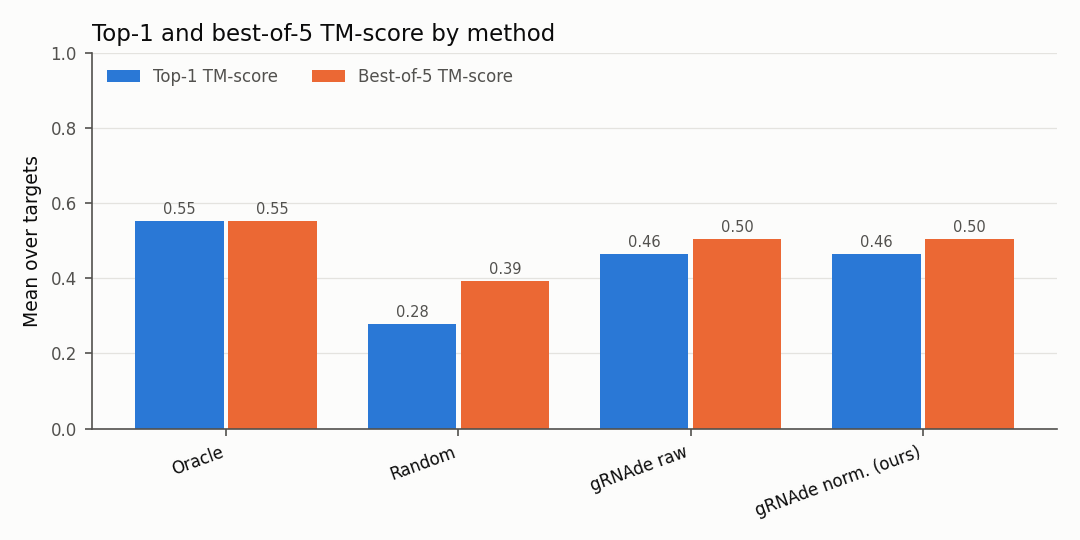
\includegraphics[width=0.8\textwidth]{Figures/grnade_selection_methods.png}}{\fbox{\parbox[c][5cm][c]{0.8\textwidth}{\centering Figure file not yet added: Figures/grnade\_selection\_methods.png}}}
\caption{Mean top-1 and best-of-5 TM-score of each selection method over all 13 targets}
\label{fig:res-selection}
\end{figure}

The validation engine is a strong selector. Over all 13 targets, its top-1 pick has a mean TM-score of 0.464, against 0.279 for a random pick and 0.552 for the oracle, so it recovers about 68\% of the gap between random selection and perfect selection. On the 6 targets with no possible training overlap, the top-1 TM-score is 0.509 against 0.281 for random and 0.649 for the oracle, recovering about 62\% of that gap, so the engine's advantage does not depend on targets gRNAde may have seen during training. When the five structures shown to the user are considered, the best of them reaches 0.505 on all targets and 0.570 on the no-overlap targets, only 0.047 and 0.079 below the oracle. Within each target, the engine's scores correlate with true quality with a mean Spearman correlation of 0.519 on all targets and 0.602 on the no-overlap targets.

\subsection{Ranking Within a Target}

% TODO: add Figures/grnade_R1128_scatter.png (the placeholder box shows until the file exists)
\begin{figure}[H]
\centering
\IfFileExists{Figures/grnade_R1128_scatter.png}{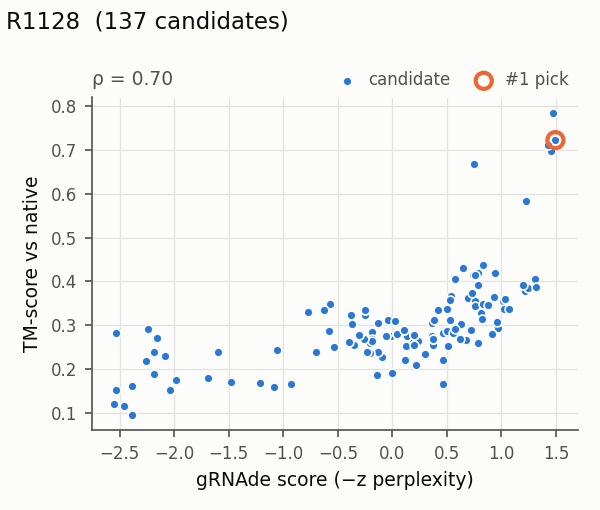
\includegraphics[width=0.8\textwidth]{Figures/grnade_R1128_scatter.png}}{\fbox{\parbox[c][5cm][c]{0.8\textwidth}{\centering Figure file not yet added: Figures/grnade\_R1128\_scatter.png}}}
\caption{gRNAde score against true TM-score for the 137 candidates of target R1128 (Spearman $\rho = 0.70$); the circled point is the engine's top pick}
\label{fig:res-r1128}
\end{figure}

Figure~\ref{fig:res-r1128} shows the behaviour of the engine on a single target, R1128, which has 137 candidate structures. Candidates with a higher gRNAde score (lower normalised perplexity) clearly tend to have higher TM-scores, with a Spearman correlation of 0.70. The engine's top pick has a TM-score of about 0.72, close to the best candidate of about 0.78, while most candidates lie between 0.2 and 0.4. This illustrates the main strength of the engine: even when most candidates are poor, it is able to pick out one of the few good ones.

\subsection{Statistical Comparison}
Table~\ref{tab:res-paired} compares the top-1 TM-scores of our method with the random pick and with raw perplexity, using a Wilcoxon signed-rank test over targets.

{\footnotesize\sloppy
\setlength{\tabcolsep}{3pt}
\begin{longtable}{|p{4.8cm}|p{2.0cm}|p{2.0cm}|p{3.0cm}|p{2.4cm}|}
\caption{Paired comparisons of top-1 TM-score (Wilcoxon signed-rank test)}\label{tab:res-paired}\\
\hline
\textbf{Comparison} & \textbf{Subset (targets)} & \textbf{Mean difference} & \textbf{Ours better / other better / ties} & \textbf{p-value}\\
\hline
\endfirsthead
\multicolumn{5}{l}{\textit{Table \thetable\ (continued)}}\\
\hline
\textbf{Comparison} & \textbf{Subset (targets)} & \textbf{Mean difference} & \textbf{Ours better / other better / ties} & \textbf{p-value}\\
\hline
\endhead
\multicolumn{5}{r}{\textit{Continued on next page}}\\
\endfoot
\endlastfoot
gRNAde normalised (ours) vs random pick & All (13) & 0.185 & 12 / 1 / 0 & 0.0005 \\ \hline
gRNAde normalised (ours) vs gRNAde raw perplexity & All (13) & 0.000 & 0 / 0 / 13 & n/a (identical picks) \\ \hline
gRNAde normalised (ours) vs random pick & No overlap (6) & 0.228 & 5 / 1 / 0 & 0.0625 \\ \hline
gRNAde normalised (ours) vs gRNAde raw perplexity & No overlap (6) & 0.000 & 0 / 0 / 6 & n/a (identical picks) \\ \hline
\end{longtable}
}

The engine beats random selection on 12 of the 13 targets, and the difference is highly significant (p = 0.0005). On the 6 no-overlap targets it is better on 5 of 6 with a larger mean difference of 0.228, but with only six targets the test cannot reach significance (p = 0.0625); this reflects the small sample, not a lack of effect. Raw and normalised perplexity give exactly the same picks on every target. This is expected by construction, because the z-score within a target preserves the order of the perplexities. Normalisation therefore does not change which candidate is chosen for a target; its purpose is to make scores comparable across different RNAs. On this data, however, pooled Spearman was slightly lower for the normalised scores (0.511 against 0.561 on all targets, and 0.588 against 0.620 on the no-overlap targets), so the expected benefit of normalisation for cross-target comparison was not observed with this small set of targets.

\subsection{Confidence Calibration}
The confidence label shown in the web application was calibrated by leave-one-target-out cross-validation. Each target's true label was set to high if the TM-score of the engine's top pick was at least 0.45, medium if it was at least 0.30, and low otherwise, and the raw perplexity of the top pick was used to predict this label, with thresholds fitted on the other twelve targets each time. The leave-one-target-out accuracy was 0.538 over the 13 targets, compared with a training accuracy of 0.769 when thresholds were fitted on all targets. The final fitted thresholds place a prediction in the high band when its perplexity is at most 2.232; the fitted medium threshold coincides with the high threshold, so in practice the label separates high from low confidence only. With so few targets, these thresholds are rough, and the confidence label should be treated as a coarse guide rather than a precise estimate of accuracy.

\subsection{Discussion}
The results show that zero-shot gRNAde perplexity is an effective way to choose among predicted RNA structures without knowing the true structure. It recovers about two thirds of the possible gain over random selection, its advantage holds on targets it cannot have seen during training, and the five structures it presents almost always include one close to the best available. This supports its role in our pipeline as the component that ranks the candidates of our RNAPro model and selects the structures shown to the user. Two weaknesses were found. First, within-target normalisation does not change the per-target ranking, and on this data it did not improve the pooled correlation either, so its value for cross-target comparison remains to be shown on a larger set of targets. Second, the confidence calibration is weak: a leave-one-target-out accuracy of 0.538 shows that a single perplexity threshold does not reliably predict whether a prediction is correct, and the medium band collapses with the fitted thresholds. Both weaknesses are mainly a consequence of the small number of evaluation targets. They will be addressed by evaluating on more targets, by calibrating confidence on the normalised score and on additional features, and by combining gRNAde with the lociPARSE quality score as planned.

\section{Discussion}
These results answer the central question of the project. Better template discovery and selection do improve RNA 3D structure prediction. With the same prediction model, our framework raises the best-of-5 TM-score from 0.553 with MMseqs2 templates and 0.621 with the paper's template pool to 0.651, and the improvement is concentrated on the template-poor RNAs that existing pipelines handle worst. The ablations show that this gain comes from combining complementary methods and learning which templates to trust, and that it does not depend on any single method.

Several limitations have to be kept in mind. The temporal test set is small, so differences of 0.01 between conditions are within the noise of individual targets and only the larger gains can be considered reliable. Our reproduced baseline is slightly below the published figure, which is why we compare mainly against our own baseline and not the paper's number. All gains are also bounded by the best available template. On targets where no good template exists in the PDB, no selector can produce an accurate structure, and the remaining gap to the upper bound shows how much room is left. Finally, the results are retrospective, and a prospective blind test on newly released structures is needed to confirm them.

\section{Conclusion}
Our experiments show that the template-finding framework finds better templates than any single method, including the first-place Kaggle search, and that these templates lead to better structures from our RNAPro model. The largest gains appear on template-poor RNAs and on the family-held-out split. Every template-finding method contributes, both new learned retrieval methods passed their acceptance checks and add measurable value, and the learned selector outperforms the heuristic picker. The choice of language model matters far less than the choice of templates, and the gRNAde-based validation engine gives confidence values that track real accuracy. Together, these results support the central claim of this project: template finding is the decisive factor in RNA 3D structure prediction, and improving it improves the final structures.

\clearpage
\chapter{Conclusions}
\label{ch:conclusions}
This chapter brings together the work we carried out during FYP-1 and the conclusions of the earlier chapters. We summarise what was built, what has been established so far and how much of the planned scope and objectives was covered, and then go through the challenges we faced and what was left out and why. The chapter closes with recommendations for future work and the plan for FYP-2.

\section{Summary of the Work Done}
The project set out to answer one question: can better template discovery and selection improve RNA 3D structure prediction? The literature reviewed in Chapter~\ref{ch:litreview} showed that templates are the most important input to the best current predictors and that prediction accuracy closely follows the quality of the best template available. It also showed that no single search method finds the right template for every RNA, and that gap shaped the whole project. Our central contribution is therefore a template-finding layer of our own. It has three parts: six complementary search methods that we implemented (sequence search, covariance-model homology, family lookup, language-model embedding similarity, secondary-structure-aware search and motif search), two new learned retrieval methods (a two-tower retriever with a learned aligner and a sequence-to-structural-token retriever), and a learned selector that decides which templates to trust for each RNA.

To measure how template choice affects the final structure, we implemented and trained our own RNAPro model, which turns the selected templates, the MSA and language-model features into five predicted C1$'$ structures. Around these two cores we built the supporting system described in Chapters~\ref{ch:srs} to~\ref{ch:impl}. This includes a data layer that enforces leakage-free temporal and family-held-out splits, a label generator that computes and caches US-align and RiboSeek labels, and a 3D validation engine based on gRNAde that ranks candidate structures and gives each prediction a confidence level. We also built a controlled framework for comparing RNA language models, along with a web application where researchers and doctors can submit sequences, follow jobs, view 2D and 3D structures, revisit past runs and ask questions about a prediction. Chapter~\ref{ch:impl} documented the implementation, the platform and APIs, and the seventeen test cases that check each component.

\section{Findings and Results}
The main finding of the design and implementation work is that template finding can be organised as a set of independent, interchangeable methods behind one common interface. Every method returns candidates in the same format, recording the source structure, the finding method, the native score, the rank and the residue mapping. Because of this, any method can be evaluated alone or in combination, and the selector can learn from information that single-method pipelines throw away, such as how many methods agree on a template. Our second finding is that enforcing the data split in the data layer, and not separately in each component, gives us a single point that can be tested for leakage, and this is what makes later comparisons trustworthy. A third finding concerns the representation gap between our RNAPro model, which outputs only C1$'$ atoms, and gRNAde, which needs backbone atoms. This gap can be bridged by full-backbone reconstruction from the C1$'$ trace, which lets an inverse-folding model act as a confidence signal without any experimental structure.

The quantitative results of the prototype are reported against the reference points set out in Chapter~\ref{ch:vision}: the published MMseqs2-only baseline (0.321), RNAPro's reported mean TM-score (0.640 in the paper's text and 0.648 in its Table 2), the best-prior-template upper bound (0.679), and our own reproduced RNAPro baseline. The measured results of our methods are given in Section~\ref{sec:testmetrics} and Chapter~\ref{ch:results}. We report results on the template-poor targets and on the family-held-out split separately, since these are the cases our framework is designed to help most.

\section{Coverage of Scope and Objectives}
\label{sec:coverage}
The objectives stated in Section~\ref{sec:objectives} fall into five areas. In prediction, the objectives were to train our own RNAPro model following its design and training recipe, reproduce its baseline, and produce five predicted C1$'$ structures per RNA guided by the selected templates. In template discovery, we aimed to build the complementary search methods behind a common interface, implement the first-place Kaggle search as the comparison baseline, record the finding method, native score and rank of every candidate, and test each method on its own. Template selection required us to compute US-align labels for all training and validation candidates, train the learned selector with top-five selection and the zero-template fallback, and compare it with the heuristic picker. For language models, the objective was a controlled comparison of RNet2, AIDO.RNA and other models. In evaluation, the objectives were to evaluate on the temporal and family-held-out benchmarks without leakage, report TM-score, RMSD and Z-scores with template-poor targets shown separately, and compare against the published baselines and the best-template upper bound. Finally, the application objectives covered sequence input and validation, job tracking, run history and sharing, a 3D viewer with PDB download, ranked candidates and a confidence indicator, as well as the secondary features of a 2D secondary-structure viewer, chat with structure, a thermodynamic stability curve and small-molecule compatibility screening.

The core scope of the project was the template-finding layer, our RNAPro model, the evaluation framework and the web application through which results reach users. The two new learned retrieval methods and the gRNAde validation engine go beyond this core and extend the original plan. We treated the secondary application features as lower priority from the start, as stated in Section~\ref{sec:scope}.

\section{Challenges Faced}
Compute was our largest challenge. The original RNAPro study trained on eight GB300 GPUs, far beyond the hardware available to a student team, so we had to fit the training of our RNAPro model onto A100-class GPUs. We did this through bf16 mixed precision, activation checkpointing, gradient accumulation and careful checkpointing, so that interrupted jobs could resume without loss. Leakage was the second challenge. Many convenient data sources and search tools silently search the whole PDB, so every method had to be routed through the split-enforcing data layer and tested for self-hits and future structures. This added work to every component, but we needed it for honest results. We also ran into mismatches between tools: different search tools report scores on different scales, gRNAde expects backbone atoms that our model does not produce, and some language models have no pair-level output. Each of these needed a bridging step that we designed and documented ourselves. A fourth challenge was the size of the evaluation sets. The temporal benchmark used in the RNAPro paper has few targets, which limits statistical power, and we addressed this with paired tests, bootstrap intervals and per-target Z-scores. Finally, we had a short schedule for a project that spans data engineering, deep-learning training, bioinformatics tools and a full web application, so we needed a strict module-wise division of work among the three members.

\section{What Was Left Out and Why}
Some planned items were not completed in FYP-1. Items were left out for one of two reasons. Some were secondary features whose value to the research question was low compared with the core pipeline. In other cases a learned component did not meet its acceptance criterion on validation data; the go/no-go rule of Section~\ref{sec:testmetrics} then requires that the component is not used, and we report the outcome and do not hide it. Prospective blind testing on unreleased structures was also outside the scope of FYP-1, because it depends on external competition rounds that we cannot schedule.

\section{Recommendations for Future Work}
Several directions follow from this work. The first is to train our RNAPro model on templates chosen by our own selector in place of the fixed MMseqs2 and first-place pool, so that the model can adapt to the higher-quality and more diverse templates our framework provides. Retrieval and selection could also be combined into a single model trained end to end, using the cached labels and features produced in this project as training data. A third direction is to extend the structural-token approach of New Method 2 with larger structural vocabularies, or to pretrain the token predictor on predicted structures, which may help families with very few solved members. We also recommend evaluating the framework prospectively on future blind targets, such as new CASP or RNA-Puzzles rounds, as this is the strongest test of a prediction method. The gRNAde confidence signal could be fine-tuned on RNA-specific quality labels so that the confidence shown to users is better calibrated. Finally, the template-finding methods, selector and evaluation tools could be released as a standalone package, so that other researchers can reuse them with their own prediction models.

\section{Plan for FYP-2}
The work planned for FYP-2 is organised in seven phases, with durations to be agreed with the supervisor at the start of the semester. In the first phase, during weeks 1 to 3, we will complete any items from Section~\ref{sec:coverage} that remain open and fix the defects found by the test cases of Chapter~\ref{ch:impl}, so that every component passes its test cases. The second phase, during weeks 3 to 7, is the full evaluation on the temporal and family-held-out benchmarks, including the single release of the test split, all ablations and the language-model comparison, and it will produce the final results with confidence intervals. During weeks 6 to 9, the third phase, we will analyse the results by method, RNA family and template availability and write Chapter~\ref{ch:results}, Experimental Results and Discussion. The fourth phase, during weeks 7 to 11, is about hardening the web application for demonstration, which covers error handling, performance with several simultaneous users, the security of share links and the chat feature, and deployment. In the fifth phase, during weeks 10 to 12, we will write the user manual for Chapter~\ref{ch:manual}, with screenshots of every use case. We will use the sixth phase, during weeks 10 to 14, to prepare a research paper describing the template-finding framework and its results and submit it to a suitable venue. In the seventh phase, during weeks 13 to 16, we will revise the final report and prepare the final presentation and demonstration.

\section{Concluding Remarks}
This project treats template finding as the decisive factor in RNA 3D structure prediction and builds a framework around it. Several complementary search methods, two new learned retrievers and a learned selector find and choose templates, and our own RNAPro model turns them into structures. A gRNAde-based engine then judges how far each prediction can be trusted, and a web application makes the system usable by researchers and doctors. The work completed in FYP-1 provides a leakage-free, fully tested pipeline in which each part can be measured on its own, and FYP-2 will complete the evaluation and show how much of the gap to the best-template upper bound this framework can close.

{
\bibliographystyle{ieeetr}
\bibliography{fypbib} %specify your .bib file here
}
%ADD APPENDICES IF REQUIRED OTHERWISE COMMENT IT OUT


\section{Equations}
Make sure you use the math environment for writing equations.  Again, make sure you do not hard code equation numbers.  Use label and ref commands of Latex to number them and reference them.  Here is an example of (\ref{eq:energy})
\begin{equation}\label{eq:energy}
E = mc^2
\end{equation}
Note, how the equation is referenced by its equation number within brackets.  

\section{Figures}
To insert a figure, you can use the following code as template.  Here the figure is referenced using ref command of Latex.  So Figure \ref{fig:fast} is the FAST logo.  DO NOT HARD CODE FIGURE NUMBERS.  Let Latex manage them for you.

\begin{figure}[htbp]
    \centering
    
\includegraphics[width=1in]{Figures/fastlogo.png}
    \caption{\textbf{FAST Logo}}
    \label{fig:fast}
\end{figure}

\section{Tables}
Note how tables can be added in Latex.  Also, make sure you use label and ref commands to define and use table numbers.  You can use Table \ref{tbl:SomeTable} as a template to make tables, add captions to them and reference them.  DO NOT HARD CODE TABLE NUMBERS.  Let Latex manage their numbering for you.

If you are having problems in managing Latex tables, you may use Lyx \url{https://www.lyx.org/}. 


\begin{table}[hbt]

\begin{center}
\caption{\label{tbl:SomeTable} \textbf{Give a Caption to the Table.}}
\begin{tabular}{|l|c|c|} 
\hline
\textbf{No.}&\textbf{Column 1}&\textbf{Column 2}\\
\hline
1.&Some data&More data\\
\hline
2.&Some values&More values\\
\hline
\end {tabular}

\end{center}

\end{table}

\section{Pseudo Code}
When you need to explain an existing algorithm of an algorithm you devised, then you should use pseudo code notation. Given below, algorithm  \ref{algo:one}, is an example. Note how the numbering is managed by the Latex itself.

\begin{algorithm}[H]
 \KwData{this text}
 \KwResult{how to write algorithm with \LaTeX2e }
 initialization\;
 \While{not at end of this document}{
  read current\;
  \eIf{understand}{
   go to next section\;
   current section becomes this one\;
   }{
   go back to the beginning of current section\;
  }
 }
 \caption{How to write algorithms}
 \label{algo:one}
\end{algorithm}

\section{Code of Programming Languages}
If you need to add C++, Java or any other programming language's code, then you can use ``listings'' package. Following is an example. Normally, the code is only added in the appendices to avoid clutter in the document.

\begin{lstlisting}

#include <stdio.h>
#define N 10
/* Block
 * comment */

int main()
{
    int i;

    // Line comment.
    puts("Hello world!");
    
    for (i = 0; i < N; i++)
    {
        puts("LaTeX is also great for programmers!");
    }

    return 0;
}
\end{lstlisting}

\section{Recommendations for \LaTeX}
Here we are providing you with only two Latex source files.  main.tex and fypbib.bib file. You can also start a project at \url{overleaf.com} and upload the zip file of this template there and share the Latex source between your group and supervisor.  This way all of you can work on the Latex files together online.

\end{document}